\documentclass[12pt,a4paper]{article}
\usepackage{cite}
\usepackage{graphicx}
\usepackage{subcaption}
\usepackage{url}
\usepackage{stfloats}
\usepackage{array}
\usepackage{tabularx}
\usepackage{amsmath}
\usepackage{textcomp}
\usepackage[english]{babel}
\usepackage{latexsym}
\usepackage{caption}
\usepackage{hyperref}
\usepackage{siunitx}
\usepackage{listings}
\setlength{\extrarowheight}{3pt}
\usepackage{tikz}
\usepackage{pgfplots}
\usepackage{environ}
\usepackage{authblk}
\usepackage[T1]{fontenc}
\usepackage[utf8]{inputenc}
\pgfplotsset{compat=1.11}
\usepackage{listings}
\usepackage{color} %red, green, blue, yellow, cyan, magenta, black, white
\definecolor{mygreen}{RGB}{28,172,0} % color values Red, Green, Blue
\definecolor{mylilas}{RGB}{170,55,241}
\definecolor{mygray}{RGB}{0.5, 0.5, 0.5}

\newlength\figureheight 
\newlength\figurewidth 
\setlength\figureheight{6cm} 
\setlength\figurewidth{0.8 \textwidth}
\lstset{language=Matlab,%
    %basicstyle=\color{red},
		basicstyle=\scriptsize,
    breaklines=true,%
    morekeywords={matlab2tikz},
    frame=single,%
	numbers=left,%
	numberstyle=\tiny\color{mygray},%
    keywordstyle=\color{blue},%
    morekeywords=[2]{1}, keywordstyle=[2]{\color{black}},
    identifierstyle=\color{black},%
    stringstyle=\color{mylilas},
    commentstyle=\color{mygreen},%
    showstringspaces=false,%without this there will be a symbol in the places where there is a space
    %numbers=left,%
    %numberstyle={\tiny \color{black}},% size of the numbers
    numbersep=9pt, % this defines how far the numbers are from the text
    emph=[1]{for,end,break},emphstyle=[1]\color{red}, %some words to emphasise
    %emph=[2]{word1,word2}, emphstyle=[2]{style},    
}
	\title{\textbf{\texttt{Matlab}$^\text{{\fontsize{12}{1em}\textcopyright}}$ Exercise II: Active Noise Control with an FIR filter}}
	\author[$\dagger$]{Ruben \textsc{Biesheuvel}}
	\author[$\ddagger$]{Mars \textsc{Geuze}}
	\affil[$\dagger$]{Student number 4076680}
	\affil[$\ddagger$]{Student number 4109139}
	\renewcommand\Authands{ and }


\begin{document}

	\maketitle

\section*{Question 1}
\subsection*{Question 1.1}
\subsubsection*{Derivation of Wiener-Hopf}
Given are the signals $v_1$ and $v_2$ generated as follows:
\begin{align}
v_1(n) - a_1(1)v_1(n-1) &= b_1(0)g(n) - b_1(1)g(n-1);\\
v_2(n) - a_2(1)v_1(n-1) &= b_2(0)g(n) - b_2(1)g(n-1),
\end{align}
where $g(n)$ is white noise with variance $\sigma^2_g$ and with parameters as given in \autoref{tab:param}. By applying the $z$-transform, the equations can be written as systems with transfer functions:
\begin{align}\label{eq:H}
H_{v_1}(z) = \frac{V_1(z)}{G(z)} = \frac{b_1(0) - b_1(1)z^{-1}}{1 - a_1(1)z^{-1}};\\
H_{v_2}(z) = \frac{V_2(z)}{G(z)} = \frac{b_2(0) - b_2(1)z^{-1}}{1 - a_2(1)z^{-1}}.
\end{align}
The poles of $H_{v_1}(z)$ and $H_{v_2}(z)$ are $a_1(1)$ and $a_2(1)$ respectively, which are inside of the unit circle, and therefore these causal filters are stable. From this and since we are filtering white noise we can conclude that both $v_1$ and $v_2$ are WSS. 
\begin{table}
\centering
\caption{\label{tab:param}Parameters given for the generation of signals $v_1$ and $v_2$.}
\begin{tabular}{|c|c|}
\hline
$a_1(1)$ & 0.9\\\hline
$b_1(0)$ & 1\\\hline
$b_1(1)$ & 0.2\\\hline
$a_2(1)$ & 0.95\\\hline
$b_2(0)$ & 1\\\hline
$b_2(1)$ & 0.3\\\hline
\end{tabular}
\end{table}

The signal $v_2(n)$ must be filtered by a filter $W(z)$ with order $m$ in such a way that the mean-square error of the noise signal $v_1(n)$ and the output of the filter $\hat{v}_1(n)$ is minimized. To estimate the filter coefficients $\hat{w}$, the following criterium is formulated:
\begin{equation}\label{eq:minimize}
\hat{w} = \arg \min_{w} E\{e(n)e^*(n)\},
\end{equation}
with 
\begin{equation}\label{eq:e}
e(n) = v_1(n) - \hat{v}_1(n) = v_1(n) - \sum\limits_{l=0}^{m-1}w(l)v_2(n-l),
\end{equation}
The lower limit of the sum is 0, since the filter is causal.

To find $\hat{w}$ for which \autoref{eq:minimize} holds it is sufficient to solve:
\begin{equation}\label{eq:condition}
\frac{\delta}{\delta w^*(k)} E\{e(n)e^*(n)\} = E\{e(n) \frac{\delta e^*(n)}{\delta w^*(k)}\} = 0,
\end{equation}
Where $k = 0, 1, \dots, m$. Using \autoref{eq:e}, the differential in \autoref{eq:condition} can be written as: 
\begin{equation}
\frac{\delta e^*(n)}{\delta w^*(k)} = \frac{\delta}{\delta w^*(k)}\left(v^*_1(n) - \sum\limits_{l=0}^{m-1}w^*(l)v_2^*(n-l)\right) = -v_2^*(n-k)
\end{equation}
Substituting into \autoref{eq:condition} and noting that the minus sign can be discarded because the expression is equal to zero, we get:
\begin{equation}
E\{e(n)v_2^*(n-k)\} = 0,
\end{equation}
In this equation we identify $e(n)$ and use \autoref{eq:e} to get:
\begin{equation}
E\{v_1(n)v_2^*(n-k)\} - \sum\limits_{l=0}^{m-1}w(l)E\{v_2(n-l)v_2^*(n-k)\} = 0
\end{equation}
Under the assumption that $v_1$ and $v_2$ are jointly WSS, $E\{v_2(n-l)v_2^*(n-k)\} = r_{v_{2}}(k-l)$ and
$E\{v_1(n)v_2^*(n - k)\} = r_{v_{1}v_{2}}(k)$, so that
\begin{equation}
\sum\limits_{l=0}^{m-1}w(l)r_{v_{2}}(k-l) = r_{v_{1}v_{2}}(k)
\end{equation}
These equations are known as the \emph{Wiener-Hopf equations}. We will now derive the expressions for $r_{v_2}(k)$ and $r_{v_{1}v_{2}}(k)$, so that $\hat{w}$ can be determined. 

\subsubsection*{Derivation of $r_{v_2}$}
First we note that $r(-k)$ is $r(k)$, since $v_1$ and $v_2$ and their correlation functions are real. Since $v_2$ is generated by an ARMA(1,1) process (i.e. $a_2(k)=0$ for $k>1$), $r(-k)$ can be derived using the \emph{Yule-Walker equations}:	
\begin{equation}\label{eq:yule}
\begin{bmatrix}
  r_{v_2}(0) & r_{v_2}(1)\\
  r_{v_2}(1) & r_{v_2}(0)
\end{bmatrix}
\begin{bmatrix}
  1\\
  a_2(1)
\end{bmatrix}
=
\sigma_g^2
\begin{bmatrix}
  c_q(1)\\
  c_q(2)
\end{bmatrix},
\end{equation}
where $c_q(k)$ is given by:
\begin{equation}\label{eq:c}
c_q(k) = \sum\limits_{l=0}^{1}b_2(l+k)h(l)
\end{equation}

By substitution of the second equation of \autoref{eq:yule} into the first one, we derive the expressions for $r_{v_2}(0)$ and $r_{v_2}(1)$:
\begin{align}\label{eq:rv2}
r_{v_2}(0) &= \frac{\sigma^2_{g}(c(1) - a_2(1)c(2))}{1-a_2(1)^2};\\
r_{v_2}(1) &= \sigma^2_{g}c(2) - a_2(1)r_{v_2}(0).
\end{align}
All subsequent values of $r_{v_2}(k)$ can be evaluated by using the following recursion formula:
\begin{equation}\label{eq:recursion}
r_{v_2}(k) = -a(1)r_{v_2}(k-1).
\end{equation}

\subsubsection*{Derivation of $r_{v_{1}v_{2}}$}
The power spectrum $P_{v_1v_2}$ can be written in terms of filter functions $H_{v_i}$:
\begin{equation}\label{eq:power}
P_{v_1v_2}(z) = H_{v_1}(z)H^{-1}_{v_2}(z)P_{v_2}(z)
\end{equation}
The expressions for $H_{v_1}(z)$ and $H^{-1}_{v_2}(z)$ are given in \autoref{eq:H}, and the product can be written as:
\begin{equation}\label{eq:HH-1}
H_{v_1}(z)H^{-1}_{v_2}(z) = \frac{b_1(0) - (b_1(0)a_2(1) + b_1(1))z^{-1} + b_1(1)a_2(1)z^{-2}}{b_2(0) - (a_1(1)b_2(0) + b_2(1))z^{-1} + a_1(1)b_2(1)z^{-2}}
\end{equation}
We can now take the inverse $z$-transform of \autoref{eq:power}, to get an expression for $r_{v_{1}v_{2}}$:
\begin{align*}\label{eq:rv1v2}
r_{v_{1}v_{2}}(n) = &b_1(0)r_{v_2}(n) - (b_1(0)a_2(1) + b_1(1))r_{v_2}(n-1) + b_1(1)a_2(1)r_{v_2}(n-2)\\
+ &(a_1(1)b_2(0) + b_2(1)) r_{v_{1}v_{2}}(n-1) - a_1(1)b_2(1)r_{v_{1}v_{2}}(n-2)
\end{align*}


\subsection*{Question 1.2}
\label{code1}
\lstinputlisting{m/Exercise_1.m}
\begin{table}[h!]
\centering
\caption{Output coefficients $w(j)$ for the optimal FIR Wiener filter}
\begin{tabular}{l r r r r}
\hline
 & \multicolumn{4}{c}{Filter order $m$}\\
 \cline{2-5}
Coefficient $w(j)$ & \num{1} & \num{2} & \num{4} & \num{6} \\
\hline
$w(0)$ & \num{0.7759} & \num{0.9209}& \num{0.9935} & \num{0.9995} \\
$w(1)$ & \num{0} & \num{-0.1623}& \num{0.0327}& \num{0.0487} \\
$w(2)$ & \num{0}& \num{0}& \num{-0.0765}& \num{-0.0242}\\
$w(3)$ & \num{0}& \num{0}& \num{-0.2255}& \num{-0.0514}\\
$w(4)$ & \num{0}& \num{0}& \num{0}& \num{-0.0859}\\
$w(5)$ & \num{0}& \num{0}& \num{0}& \num{-0.1916}\\
\hline
\end{tabular}
\end{table}

\clearpage\section*{Question 2}

\begin{table}[h!]
\centering
\caption{Standard deviation $\sigma_{W}$ between the sound $d(n)$ and the estimated sound $x(n) - \hat{v_{1}}(n)$}
\begin{tabular}{l | r}
Filter order $m$ & $\sigma_{W}$ \\
\hline
\num{1} & \num{0.2075}\\
\num{2} & \num{0.1996}\\
\num{4} & \num{0.1674}\\
\num{6} & \num{0.1362}\\
\hline
\end{tabular}
\end{table}

\begin{figure}[h!]
\centering
% This file was created by matlab2tikz.
% Minimal pgfplots version: 1.3
%
%The latest updates can be retrieved from
%  http://www.mathworks.com/matlabcentral/fileexchange/22022-matlab2tikz
%where you can also make suggestions and rate matlab2tikz.
%
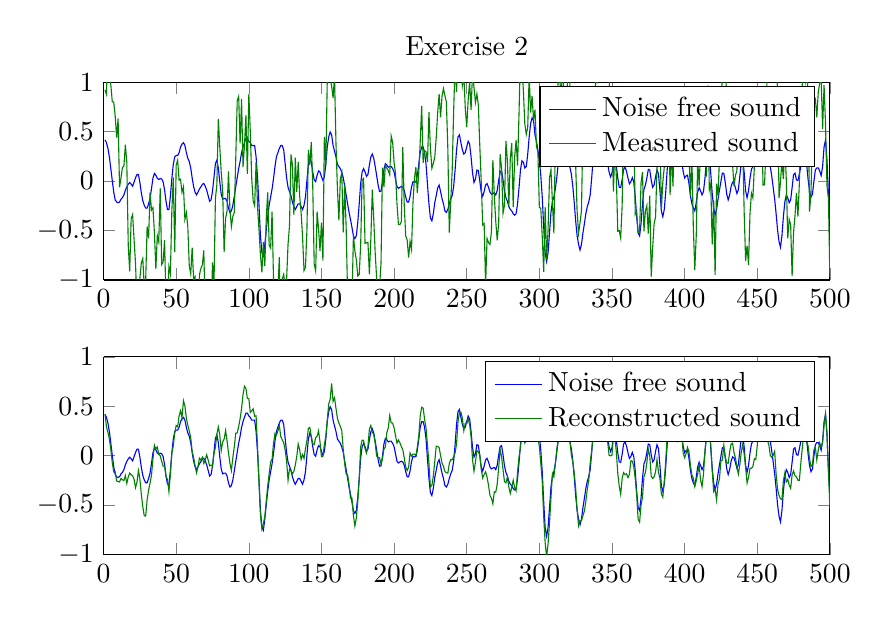
\begin{tikzpicture}

\begin{axis}[%
width=0.95092\figurewidth,
height=0.418605\figureheight,
at={(0\figurewidth,0\figureheight)},
scale only axis,
separate axis lines,
every outer x axis line/.append style={black},
every x tick label/.append style={font=\color{black}},
xmin=0,
xmax=500,
every outer y axis line/.append style={black},
every y tick label/.append style={font=\color{black}},
ymin=-1,
ymax=1,
legend style={legend cell align=left,align=left,draw=black}
]
\addplot [color=blue,solid]
  table[row sep=crcr]{%
1	0.417135147290308\\
2	0.38835169777378\\
3	0.330784798740724\\
4	0.24443445019114\\
5	0.125702720935462\\
6	0.00494715538565325\\
7	-0.111310996177198\\
8	-0.19046548234765\\
9	-0.212053069485046\\
10	-0.219248931864178\\
11	-0.212053069485046\\
12	-0.183269619968518\\
13	-0.168877895210254\\
14	-0.140094445693726\\
15	-0.0915223746345851\\
16	-0.0591409939284911\\
17	-0.0312570272093546\\
18	-0.0146165954576119\\
19	-0.0312570272093546\\
20	-0.0519451315493591\\
21	-0.0101191814706544\\
22	0.0330559928041376\\
23	0.0663368563076231\\
24	0.0663368563076231\\
25	-0.0137171126602204\\
26	-0.11850685855633\\
27	-0.197661344726782\\
28	-0.24443445019114\\
29	-0.273217899707668\\
30	-0.273217899707668\\
31	-0.230042725432876\\
32	-0.176073757589386\\
33	-0.0771306498763211\\
34	0.0294580616145716\\
35	0.0771306498763211\\
36	0.0591409939284911\\
37	0.0276590960197886\\
38	0.0155160782550034\\
39	0.0258601304250056\\
40	0.0209129750393524\\
41	-0.00832021587587137\\
42	-0.0879244434450191\\
43	-0.204857207105914\\
44	-0.287609624465932\\
45	-0.287609624465932\\
46	-0.15448617045199\\
47	0.0258601304250056\\
48	0.168877895210254\\
49	0.24443445019114\\
50	0.258826174949404\\
51	0.258826174949404\\
52	0.287609624465932\\
53	0.345176523498988\\
54	0.373959973015516\\
55	0.38835169777378\\
56	0.359568248257252\\
57	0.287609624465932\\
58	0.230042725432876\\
59	0.197661344726782\\
60	0.132898583314594\\
61	0.0312570272093546\\
62	-0.0555430627389251\\
63	-0.111310996177198\\
64	-0.140094445693726\\
65	-0.111310996177198\\
66	-0.0807285810658871\\
67	-0.0591409939284911\\
68	-0.0330559928041376\\
69	-0.0240611648302226\\
70	-0.0519451315493591\\
71	-0.0915223746345851\\
72	-0.147290308072858\\
73	-0.204857207105914\\
74	-0.19046548234765\\
75	-0.102316168203283\\
76	0.0366539239937036\\
77	0.176073757589386\\
78	0.212053069485046\\
79	0.132898583314594\\
80	-0.00832021587587137\\
81	-0.132898583314594\\
82	-0.183269619968518\\
83	-0.176073757589386\\
84	-0.176073757589386\\
85	-0.204857207105914\\
86	-0.273217899707668\\
87	-0.31639307398246\\
88	-0.302001349224196\\
89	-0.24443445019114\\
90	-0.15448617045199\\
91	-0.0591409939284911\\
92	0.0330559928041376\\
93	0.125702720935462\\
94	0.197661344726782\\
95	0.287609624465932\\
96	0.345176523498988\\
97	0.38835169777378\\
98	0.431526872048572\\
99	0.431526872048572\\
100	0.402743422532044\\
101	0.38835169777378\\
102	0.359568248257252\\
103	0.359568248257252\\
104	0.359568248257252\\
105	0.24443445019114\\
106	0.0366539239937036\\
107	-0.24443445019114\\
108	-0.553856532493816\\
109	-0.726557229592984\\
110	-0.755340679109512\\
111	-0.6402068810434\\
112	-0.49628963346076\\
113	-0.359568248257252\\
114	-0.24443445019114\\
115	-0.161682032831122\\
116	-0.0807285810658871\\
117	0.0240611648302226\\
118	0.147290308072858\\
119	0.24443445019114\\
120	0.287609624465932\\
121	0.330784798740724\\
122	0.359568248257252\\
123	0.359568248257252\\
124	0.31639307398246\\
125	0.176073757589386\\
126	0.0330559928041376\\
127	-0.0627389251180571\\
128	-0.105914099392849\\
129	-0.147290308072858\\
130	-0.212053069485046\\
131	-0.258826174949404\\
132	-0.287609624465932\\
133	-0.258826174949404\\
134	-0.230042725432876\\
135	-0.230042725432876\\
136	-0.258826174949404\\
137	-0.287609624465932\\
138	-0.24443445019114\\
139	-0.161682032831122\\
140	0.00584663818304475\\
141	0.168877895210254\\
142	0.230042725432876\\
143	0.19046548234765\\
144	0.0915223746345851\\
145	0.0128176298628289\\
146	-0.005396896784349\\
147	0.0591409939284911\\
148	0.102316168203283\\
149	0.0915223746345851\\
150	0.0438497863728356\\
151	0.0062963795817405\\
152	0.0420508207780526\\
153	0.168877895210254\\
154	0.345176523498988\\
155	0.445918596806836\\
156	0.49628963346076\\
157	0.467506183944232\\
158	0.359568248257252\\
159	0.302001349224196\\
160	0.24443445019114\\
161	0.168877895210254\\
162	0.147290308072858\\
163	0.125702720935462\\
164	0.0879244434450191\\
165	0.0348549583989206\\
166	-0.0519451315493591\\
167	-0.140094445693726\\
168	-0.230042725432876\\
169	-0.31639307398246\\
170	-0.38835169777378\\
171	-0.467506183944232\\
172	-0.553856532493816\\
173	-0.582639982010344\\
174	-0.553856532493816\\
175	-0.417135147290308\\
176	-0.230042725432876\\
177	-0.0240611648302226\\
178	0.0915223746345851\\
179	0.125702720935462\\
180	0.0915223746345851\\
181	0.0474477175624016\\
182	0.0663368563076231\\
183	0.161682032831122\\
184	0.24443445019114\\
185	0.273217899707668\\
186	0.230042725432876\\
187	0.147290308072858\\
188	0.0555430627389251\\
189	-0.0384528895884866\\
190	-0.105914099392849\\
191	-0.102316168203283\\
192	-0.00404767258826175\\
193	0.11850685855633\\
194	0.176073757589386\\
195	0.161682032831122\\
196	0.140094445693726\\
197	0.147290308072858\\
198	0.147290308072858\\
199	0.125702720935462\\
200	0.0915223746345851\\
201	0.0182145266471779\\
202	-0.0555430627389251\\
203	-0.0735327186867551\\
204	-0.0627389251180571\\
205	-0.0555430627389251\\
206	-0.0627389251180571\\
207	-0.0951203058241511\\
208	-0.161682032831122\\
209	-0.212053069485046\\
210	-0.212053069485046\\
211	-0.15448617045199\\
212	-0.0591409939284911\\
213	-0.00674612098043625\\
214	-0.0110186642680459\\
215	-0.00921969867326287\\
216	0.0555430627389251\\
217	0.168877895210254\\
218	0.287609624465932\\
219	0.345176523498988\\
220	0.345176523498988\\
221	0.287609624465932\\
222	0.168877895210254\\
223	-0.0366539239937036\\
224	-0.230042725432876\\
225	-0.373959973015516\\
226	-0.402743422532044\\
227	-0.330784798740724\\
228	-0.219248931864178\\
229	-0.147290308072858\\
230	-0.0699347874971891\\
231	-0.0402518551832696\\
232	-0.105914099392849\\
233	-0.176073757589386\\
234	-0.230042725432876\\
235	-0.302001349224196\\
236	-0.31639307398246\\
237	-0.287609624465932\\
238	-0.230042725432876\\
239	-0.183269619968518\\
240	-0.147290308072858\\
241	-0.0555430627389251\\
242	0.111310996177198\\
243	0.31639307398246\\
244	0.445918596806836\\
245	0.467506183944232\\
246	0.38835169777378\\
247	0.31639307398246\\
248	0.273217899707668\\
249	0.287609624465932\\
250	0.345176523498988\\
251	0.402743422532044\\
252	0.373959973015516\\
253	0.24443445019114\\
254	0.0843265122554531\\
255	-0.0137171126602204\\
256	0.0200134922419609\\
257	0.111310996177198\\
258	0.105914099392849\\
259	-0.00044974139869575\\
260	-0.111310996177198\\
261	-0.15448617045199\\
262	-0.105914099392849\\
263	-0.0402518551832696\\
264	-0.0258601304250056\\
265	-0.0627389251180571\\
266	-0.111310996177198\\
267	-0.132898583314594\\
268	-0.125702720935462\\
269	-0.11850685855633\\
270	-0.140094445693726\\
271	-0.0951203058241511\\
272	0.00584663818304475\\
273	0.0915223746345851\\
274	0.102316168203283\\
275	0.0110186642680459\\
276	-0.102316168203283\\
277	-0.168877895210254\\
278	-0.204857207105914\\
279	-0.258826174949404\\
280	-0.287609624465932\\
281	-0.302001349224196\\
282	-0.330784798740724\\
283	-0.345176523498988\\
284	-0.330784798740724\\
285	-0.230042725432876\\
286	-0.0699347874971891\\
287	0.111310996177198\\
288	0.204857207105914\\
289	0.19046548234765\\
290	0.132898583314594\\
291	0.147290308072858\\
292	0.273217899707668\\
293	0.445918596806836\\
294	0.582639982010344\\
295	0.6402068810434\\
296	0.611423431526872\\
297	0.467506183944232\\
298	0.402743422532044\\
299	0.31639307398246\\
300	0.204857207105914\\
301	0.0555430627389251\\
302	-0.161682032831122\\
303	-0.467506183944232\\
304	-0.726557229592984\\
305	-0.812907578142568\\
306	-0.726557229592984\\
307	-0.525073082977288\\
308	-0.31639307398246\\
309	-0.204857207105914\\
310	-0.161682032831122\\
311	-0.0807285810658871\\
312	0.0348549583989206\\
313	0.176073757589386\\
314	0.345176523498988\\
315	0.525073082977288\\
316	0.611423431526872\\
317	0.553856532493816\\
318	0.431526872048572\\
319	0.287609624465932\\
320	0.183269619968518\\
321	0.140094445693726\\
322	0.0735327186867551\\
323	-0.0474477175624016\\
324	-0.212053069485046\\
325	-0.402743422532044\\
326	-0.553856532493816\\
327	-0.6402068810434\\
328	-0.697773780076456\\
329	-0.6402068810434\\
330	-0.525073082977288\\
331	-0.431526872048572\\
332	-0.330784798740724\\
333	-0.258826174949404\\
334	-0.212053069485046\\
335	-0.140094445693726\\
336	0.0240611648302226\\
337	0.219248931864178\\
338	0.359568248257252\\
339	0.417135147290308\\
340	0.417135147290308\\
341	0.417135147290308\\
342	0.402743422532044\\
343	0.359568248257252\\
344	0.330784798740724\\
345	0.330784798740724\\
346	0.287609624465932\\
347	0.183269619968518\\
348	0.0915223746345851\\
349	0.0420508207780526\\
350	0.0807285810658871\\
351	0.197661344726782\\
352	0.24443445019114\\
353	0.15448617045199\\
354	0.0294580616145716\\
355	-0.0627389251180571\\
356	-0.0663368563076231\\
357	0.0146165954576119\\
358	0.11850685855633\\
359	0.140094445693726\\
360	0.0987182370137171\\
361	0.0312570272093546\\
362	-0.0276590960197886\\
363	-0.00742073307847987\\
364	0.0348549583989206\\
365	-0.00921969867326287\\
366	-0.15448617045199\\
367	-0.359568248257252\\
368	-0.525073082977288\\
369	-0.553856532493816\\
370	-0.431526872048572\\
371	-0.230042725432876\\
372	-0.0843265122554531\\
373	-0.0420508207780526\\
374	0.0294580616145716\\
375	0.11850685855633\\
376	0.111310996177198\\
377	0.0110186642680459\\
378	-0.0627389251180571\\
379	-0.0402518551832696\\
380	0.0438497863728356\\
381	0.111310996177198\\
382	0.0735327186867551\\
383	-0.0951203058241511\\
384	-0.302001349224196\\
385	-0.359568248257252\\
386	-0.287609624465932\\
387	-0.111310996177198\\
388	0.111310996177198\\
389	0.273217899707668\\
390	0.302001349224196\\
391	0.24443445019114\\
392	0.19046548234765\\
393	0.212053069485046\\
394	0.287609624465932\\
395	0.31639307398246\\
396	0.31639307398246\\
397	0.287609624465932\\
398	0.204857207105914\\
399	0.0987182370137171\\
400	0.0312570272093546\\
401	0.0519451315493591\\
402	0.0591409939284911\\
403	-0.0258601304250056\\
404	-0.147290308072858\\
405	-0.230042725432876\\
406	-0.273217899707668\\
407	-0.302001349224196\\
408	-0.219248931864178\\
409	-0.111310996177198\\
410	-0.0663368563076231\\
411	-0.0987182370137171\\
412	-0.140094445693726\\
413	-0.105914099392849\\
414	0.0276590960197886\\
415	0.204857207105914\\
416	0.330784798740724\\
417	0.273217899707668\\
418	0.0771306498763211\\
419	-0.125702720935462\\
420	-0.273217899707668\\
421	-0.345176523498988\\
422	-0.287609624465932\\
423	-0.183269619968518\\
424	-0.0915223746345851\\
425	-0.003597931189566\\
426	0.0807285810658871\\
427	0.0771306498763211\\
428	-0.0146165954576119\\
429	-0.132898583314594\\
430	-0.19046548234765\\
431	-0.140094445693726\\
432	-0.0555430627389251\\
433	-0.0119181470654374\\
434	-0.0209129750393524\\
435	-0.0699347874971891\\
436	-0.125702720935462\\
437	-0.0879244434450191\\
438	0.0492466831571846\\
439	0.183269619968518\\
440	0.219248931864178\\
441	0.0879244434450191\\
442	-0.0987182370137171\\
443	-0.168877895210254\\
444	-0.0987182370137171\\
445	0.0258601304250056\\
446	0.11850685855633\\
447	0.147290308072858\\
448	0.168877895210254\\
449	0.168877895210254\\
450	0.219248931864178\\
451	0.359568248257252\\
452	0.525073082977288\\
453	0.582639982010344\\
454	0.525073082977288\\
455	0.38835169777378\\
456	0.258826174949404\\
457	0.204857207105914\\
458	0.19046548234765\\
459	0.147290308072858\\
460	0.0474477175624016\\
461	-0.0663368563076231\\
462	-0.183269619968518\\
463	-0.330784798740724\\
464	-0.49628963346076\\
465	-0.611423431526872\\
466	-0.668990330559928\\
467	-0.553856532493816\\
468	-0.359568248257252\\
469	-0.212053069485046\\
470	-0.140094445693726\\
471	-0.168877895210254\\
472	-0.219248931864178\\
473	-0.19046548234765\\
474	-0.0663368563076231\\
475	0.0663368563076231\\
476	0.0807285810658871\\
477	0.0119181470654374\\
478	0.005396896784349\\
479	0.0699347874971891\\
480	0.147290308072858\\
481	0.24443445019114\\
482	0.345176523498988\\
483	0.31639307398246\\
484	0.168877895210254\\
485	0.0191140094445694\\
486	-0.0987182370137171\\
487	-0.161682032831122\\
488	-0.132898583314594\\
489	-0.00404767258826175\\
490	0.111310996177198\\
491	0.132898583314594\\
492	0.132898583314594\\
493	0.102316168203283\\
494	0.0555430627389251\\
495	0.147290308072858\\
496	0.345176523498988\\
497	0.417135147290308\\
498	0.219248931864178\\
499	-0.140094445693726\\
500	-0.402743422532044\\
501	-0.402743422532044\\
};
\addlegendentry{Noise free sound};

\addplot [color=black!50!green,solid]
  table[row sep=crcr]{%
1	0.420691879742161\\
2	0.294023198415202\\
3	0.237404930791248\\
4	0.169970255554796\\
5	0.06350141128569\\
6	-0.0698406214026389\\
7	-0.163213615593082\\
8	-0.159087248579799\\
9	-0.253879252410031\\
10	-0.260982015054769\\
11	-0.265105127600363\\
12	-0.229664900719881\\
13	-0.243281186929488\\
14	-0.250157230186728\\
15	-0.199363188804522\\
16	-0.278862572433287\\
17	-0.214715589585986\\
18	-0.176533182429363\\
19	-0.191351243710324\\
20	-0.203244582639438\\
21	-0.236993494094151\\
22	-0.32278782870064\\
23	-0.266667373280685\\
24	-0.149757682820259\\
25	-0.233408562465641\\
26	-0.392625179584475\\
27	-0.514259374573085\\
28	-0.606481235177597\\
29	-0.609123097921497\\
30	-0.4454260832537\\
31	-0.349519494339191\\
32	-0.277078513855278\\
33	-0.195390483281407\\
34	-0.0315866299152422\\
35	0.106761238637462\\
36	0.0679747570722449\\
37	0.0889691718677489\\
38	0.0138425306405552\\
39	0.000251566045602669\\
40	-0.0555434879988352\\
41	-0.105122473620276\\
42	-0.102992423301462\\
43	-0.211657013255171\\
44	-0.238833850937048\\
45	-0.364078210736358\\
46	-0.189516259438611\\
47	0.0280044657242675\\
48	0.100371860544809\\
49	0.228773020217688\\
50	0.306115347425113\\
51	0.292644528255574\\
52	0.402972636349029\\
53	0.45447229996617\\
54	0.384570487408763\\
55	0.556878639004077\\
56	0.50257476965278\\
57	0.379838255677909\\
58	0.30876276548202\\
59	0.250529240827621\\
60	0.185349880474541\\
61	0.0428447454308306\\
62	-0.0176512645697606\\
63	-0.0993565661624722\\
64	-0.173279628303808\\
65	-0.113623083248594\\
66	-0.0243805487996146\\
67	-0.0442431877707291\\
68	-0.0161142301134825\\
69	-0.0775288719045543\\
70	-0.0429487897583223\\
71	0.0102260401534007\\
72	-0.0435735532119113\\
73	-0.10190808907913\\
74	-0.0935812331010999\\
75	-0.107778882210924\\
76	0.019184958936949\\
77	0.0859760966902249\\
78	0.219339179470449\\
79	0.291214534775888\\
80	0.209795774808997\\
81	0.051421560428087\\
82	0.138095475271657\\
83	0.168275994930308\\
84	0.255848687434855\\
85	0.153090152591819\\
86	0.0291304508852367\\
87	-0.0746883998281511\\
88	-0.149283842841482\\
89	-0.0184940209809596\\
90	0.0906244369810533\\
91	0.227549978517233\\
92	0.231350184068141\\
93	0.292972978054235\\
94	0.37546224304861\\
95	0.477156761169245\\
96	0.617658881481012\\
97	0.703518698076943\\
98	0.681228033921041\\
99	0.581324217262584\\
100	0.577036072716243\\
101	0.437909723823579\\
102	0.454968179629375\\
103	0.473635434332415\\
104	0.39962395684936\\
105	0.402716431466701\\
106	0.0884926043338118\\
107	-0.27214701344485\\
108	-0.598202185522107\\
109	-0.741287478400747\\
110	-0.684519932976068\\
111	-0.616913215833168\\
112	-0.456436150741306\\
113	-0.307716627612491\\
114	-0.183241237118544\\
115	-0.0616821363537097\\
116	-0.0342540703239974\\
117	0.124962518548474\\
118	0.22454558954282\\
119	0.205717512889626\\
120	0.249466929782852\\
121	0.306815352983196\\
122	0.192497175393986\\
123	0.161904680067679\\
124	0.131497333094765\\
125	0.0577769744380818\\
126	-0.052925245780276\\
127	-0.246845398065434\\
128	-0.135498966068723\\
129	-0.149175476707087\\
130	-0.181574301012816\\
131	-0.158880074049233\\
132	-0.0937716692403269\\
133	-0.00808870798286174\\
134	0.118356810095545\\
135	0.0604692492414281\\
136	-0.0368827788170394\\
137	0.0115653046031973\\
138	-0.027060406040194\\
139	0.071512807442067\\
140	0.153624515327648\\
141	0.277542172605853\\
142	0.286526444560062\\
143	0.195475154052089\\
144	0.121998159591749\\
145	0.112399702613842\\
146	0.183215902258691\\
147	0.196000300400275\\
148	0.251058155684486\\
149	0.140155309236003\\
150	-0.0100050429895792\\
151	-0.00805075206763139\\
152	0.113722718079834\\
153	0.192335286762117\\
154	0.358995153382564\\
155	0.52391091831558\\
156	0.569867393022047\\
157	0.730388885894176\\
158	0.549697217453111\\
159	0.586900743749868\\
160	0.478355401419285\\
161	0.376959488191052\\
162	0.331899454936882\\
163	0.297109069287543\\
164	0.254223465937865\\
165	0.0617207966968388\\
166	-0.0837219015423553\\
167	-0.184789774486567\\
168	-0.191971363232855\\
169	-0.290482538957751\\
170	-0.433036197630918\\
171	-0.430185382509856\\
172	-0.605374314184036\\
173	-0.710327402556629\\
174	-0.632944504683388\\
175	-0.462707208779319\\
176	-0.230332246985993\\
177	0.0917864021885758\\
178	0.157829637803888\\
179	0.155878982095672\\
180	0.0732246273354902\\
181	0.0262862938564123\\
182	0.0952363293779926\\
183	0.26959066228986\\
184	0.305995107521489\\
185	0.235287697204611\\
186	0.215693180097418\\
187	0.125627450007548\\
188	-0.00425564787313792\\
189	-0.0157114047216327\\
190	-0.0222294672598002\\
191	-0.083928819653181\\
192	-0.0303798690958324\\
193	0.0662029817760616\\
194	0.0880715034976102\\
195	0.23256480456092\\
196	0.281836170536451\\
197	0.405833991712178\\
198	0.332241756031523\\
199	0.330593256866527\\
200	0.28216133300813\\
201	0.202109293760434\\
202	0.128141840758999\\
203	0.158914893147599\\
204	0.131394812670893\\
205	0.0933367165956041\\
206	0.0611912421892936\\
207	-0.0212922610947797\\
208	-0.112278293561774\\
209	-0.149778768120011\\
210	-0.117181348582833\\
211	0.0279504605896393\\
212	-0.00325444905355443\\
213	0.0167905088633616\\
214	0.0159435554931657\\
215	-0.00152185008630631\\
216	0.0872819059458934\\
217	0.19843671308244\\
218	0.403341884856421\\
219	0.490370889246427\\
220	0.481723668336722\\
221	0.369289809413551\\
222	0.278860929769228\\
223	0.105866525831231\\
224	-0.0759313251903162\\
225	-0.317028371798585\\
226	-0.300389727218067\\
227	-0.205215502890562\\
228	-0.0588652948975691\\
229	0.0958754729319945\\
230	0.0948079751669939\\
231	0.0822294058798358\\
232	0.00463965833709201\\
233	-0.0740912588793026\\
234	-0.107387905697879\\
235	-0.160002082581847\\
236	-0.171878543694053\\
237	-0.17579754607221\\
238	-0.0799078060919192\\
239	-0.0406193365741711\\
240	-0.0406907925323324\\
241	-0.00929674904617084\\
242	0.0295972566018403\\
243	0.118955125929086\\
244	0.342589115020258\\
245	0.438468150815228\\
246	0.441264018057531\\
247	0.379369022814364\\
248	0.253692297337436\\
249	0.32863244601738\\
250	0.324304427938634\\
251	0.370702845130973\\
252	0.317643175326361\\
253	0.191389124260145\\
254	-0.0394398224485366\\
255	-0.156085532425736\\
256	-0.0677949747586174\\
257	0.0531509562107803\\
258	0.0387264738354201\\
259	0.0111152458596918\\
260	-0.13824362506533\\
261	-0.224440825865125\\
262	-0.188877249608886\\
263	-0.162841977965207\\
264	-0.213150146042743\\
265	-0.299558399845129\\
266	-0.402004583921995\\
267	-0.428315109519555\\
268	-0.485957419353913\\
269	-0.363853070837136\\
270	-0.368059366145508\\
271	-0.286746638480595\\
272	-0.121019552035554\\
273	0.0635388484638401\\
274	-0.0129579927858091\\
275	-0.139471409783568\\
276	-0.262471831491714\\
277	-0.27390595930548\\
278	-0.215049968001454\\
279	-0.317409119672007\\
280	-0.381372776550857\\
281	-0.320050758747778\\
282	-0.248376450382488\\
283	-0.323711331759729\\
284	-0.35418982068227\\
285	-0.163282471394334\\
286	-0.014374353323401\\
287	0.0819012065860256\\
288	0.271980477874028\\
289	0.253654472031451\\
290	0.146630431948806\\
291	0.234361054623714\\
292	0.394626982397738\\
293	0.490431847351002\\
294	0.563840019182434\\
295	0.570234517341648\\
296	0.527802031734625\\
297	0.389605439173861\\
298	0.359454334909337\\
299	0.184532567317482\\
300	0.0959291150795386\\
301	-0.0775161635070161\\
302	-0.260881110816994\\
303	-0.619951843844263\\
304	-0.880840436862409\\
305	-1.0220830700363\\
306	-0.891126591060174\\
307	-0.680164357693509\\
308	-0.428213850856198\\
309	-0.179488396898701\\
310	-0.214565829786627\\
311	-0.082305082871869\\
312	0.0655437695091841\\
313	0.150765192222849\\
314	0.243280398782774\\
315	0.417628222645708\\
316	0.643769146957854\\
317	0.549028274651183\\
318	0.549929419754193\\
319	0.3131027266947\\
320	0.151853651200528\\
321	0.154463616870721\\
322	0.0116489222712284\\
323	-0.0625777259596229\\
324	-0.175204410303815\\
325	-0.327934626188832\\
326	-0.546747190726845\\
327	-0.708577766475518\\
328	-0.657254197859548\\
329	-0.655829786728575\\
330	-0.605645869605133\\
331	-0.561700069553621\\
332	-0.45975791802694\\
333	-0.340397273994832\\
334	-0.251857345278201\\
335	-0.0734953810196077\\
336	0.0527971141901747\\
337	0.202290681519389\\
338	0.310250272173562\\
339	0.303983890337084\\
340	0.364683922137767\\
341	0.309585952899841\\
342	0.323948499258474\\
343	0.238310854088555\\
344	0.267621304490419\\
345	0.25924360815765\\
346	0.28245353425711\\
347	0.144672064430132\\
348	0.00468181876410467\\
349	-0.000795484339605967\\
350	0.00537724043156257\\
351	0.209715972751395\\
352	0.186223858475088\\
353	0.0368202715900628\\
354	-0.179348686125392\\
355	-0.308333210711745\\
356	-0.390336924379099\\
357	-0.227363112243511\\
358	-0.171027337903148\\
359	-0.191118030668198\\
360	-0.183204095234706\\
361	-0.221484173160413\\
362	-0.18878388673196\\
363	-0.0506925999558256\\
364	-0.0553218144580309\\
365	-0.108770304058552\\
366	-0.230338713925255\\
367	-0.394120070378961\\
368	-0.642481982581326\\
369	-0.67131538491273\\
370	-0.49993390606846\\
371	-0.418907478116385\\
372	-0.213496660810085\\
373	-0.168400202738904\\
374	-0.071118655074928\\
375	0.0655129824384416\\
376	0.00243828128581206\\
377	-0.205603827189143\\
378	-0.230185601655968\\
379	-0.213213613819779\\
380	-0.165170603903392\\
381	-0.0396701510138896\\
382	-0.164255463103165\\
383	-0.229021695832666\\
384	-0.385834735907746\\
385	-0.418490851224899\\
386	-0.258622066167967\\
387	-0.0507972376365931\\
388	0.196132451915275\\
389	0.266228892459855\\
390	0.363838802090807\\
391	0.318882016215848\\
392	0.292697207978604\\
393	0.200405950882062\\
394	0.300187817867249\\
395	0.172656776282727\\
396	0.274642920623434\\
397	0.216089191203878\\
398	0.219083289384956\\
399	0.0302409566510454\\
400	-0.0213401280136747\\
401	0.0220246237810522\\
402	0.0842416892662574\\
403	0.0434362712634705\\
404	-0.0954528174053716\\
405	-0.196005032978803\\
406	-0.224525216317028\\
407	-0.310698054038436\\
408	-0.25198980179186\\
409	-0.182678688151237\\
410	-0.0893531282750837\\
411	-0.248101105921131\\
412	-0.311673710368522\\
413	-0.183836012744196\\
414	0.04913603884222\\
415	0.18097915835448\\
416	0.378940230975254\\
417	0.318961736779663\\
418	0.112227584567565\\
419	-0.151457618754439\\
420	-0.361487859127102\\
421	-0.336739873049883\\
422	-0.446457909757847\\
423	-0.286770170145881\\
424	-0.23254417234593\\
425	-0.0524489643526647\\
426	-0.0434896158150828\\
427	0.106428716846296\\
428	-0.0192712222370062\\
429	-0.0714099080953237\\
430	-0.0779380737686791\\
431	0.0391115937884393\\
432	0.119090009014088\\
433	0.126839647518398\\
434	0.032654554953725\\
435	-0.0222102690360541\\
436	-0.109997221269449\\
437	-0.18540845514208\\
438	-0.0905604132830437\\
439	0.0329656605033313\\
440	0.116153185039529\\
441	0.0175895917269361\\
442	-0.119035092298169\\
443	-0.27542923433451\\
444	-0.219102812721483\\
445	-0.127500445218313\\
446	-0.125697861374311\\
447	-0.10885480465105\\
448	-0.0306273208995591\\
449	-0.0389320834643037\\
450	0.101661597334353\\
451	0.26561751311189\\
452	0.442695274210166\\
453	0.574262560544703\\
454	0.581527025511929\\
455	0.374459338499335\\
456	0.248222624663237\\
457	0.158232845030397\\
458	0.109872703635192\\
459	0.00088490939309871\\
460	-0.0150217590181276\\
461	0.00393672939276435\\
462	0.0456864469907619\\
463	-0.186871069360571\\
464	-0.339130127635966\\
465	-0.400539407294073\\
466	-0.434218573246133\\
467	-0.444160131794803\\
468	-0.25372948951477\\
469	-0.173892352150367\\
470	-0.263684781708471\\
471	-0.239013756520146\\
472	-0.295855417366611\\
473	-0.330894596011644\\
474	-0.19248153096755\\
475	-0.153559580194507\\
476	-0.20221010034807\\
477	-0.214079237925024\\
478	-0.247175570795101\\
479	-0.248803315043136\\
480	-0.0743865054073227\\
481	0.0741164714195436\\
482	0.226978090880874\\
483	0.187213374541062\\
484	0.13258743126741\\
485	0.103212772406386\\
486	-0.0322627447179679\\
487	-0.108367251727378\\
488	-0.0911947990577567\\
489	0.0597562853886627\\
490	0.087353226002801\\
491	-0.0436770161251728\\
492	0.0561657773906238\\
493	0.129629668462166\\
494	0.0877774208445201\\
495	0.138498889919191\\
496	0.309664403414746\\
497	0.426089448978169\\
498	0.23135178394934\\
499	-0.15390735097301\\
500	-0.519328809550308\\
501	-0.495636989969925\\
};
\addlegendentry{Reconstructed sound};

\end{axis}

\begin{axis}[%
width=0.95092\figurewidth,
height=0.418605\figureheight,
at={(0\figurewidth,0.581395\figureheight)},
scale only axis,
separate axis lines,
every outer x axis line/.append style={black},
every x tick label/.append style={font=\color{black}},
xmin=0,
xmax=500,
every outer y axis line/.append style={black},
every y tick label/.append style={font=\color{black}},
ymin=-1,
ymax=1,
title={Exercise 2},
legend style={legend cell align=left,align=left,draw=black}
]
\addplot [color=blue,solid]
  table[row sep=crcr]{%
1	0.417135147290308\\
2	0.38835169777378\\
3	0.330784798740724\\
4	0.24443445019114\\
5	0.125702720935462\\
6	0.00494715538565325\\
7	-0.111310996177198\\
8	-0.19046548234765\\
9	-0.212053069485046\\
10	-0.219248931864178\\
11	-0.212053069485046\\
12	-0.183269619968518\\
13	-0.168877895210254\\
14	-0.140094445693726\\
15	-0.0915223746345851\\
16	-0.0591409939284911\\
17	-0.0312570272093546\\
18	-0.0146165954576119\\
19	-0.0312570272093546\\
20	-0.0519451315493591\\
21	-0.0101191814706544\\
22	0.0330559928041376\\
23	0.0663368563076231\\
24	0.0663368563076231\\
25	-0.0137171126602204\\
26	-0.11850685855633\\
27	-0.197661344726782\\
28	-0.24443445019114\\
29	-0.273217899707668\\
30	-0.273217899707668\\
31	-0.230042725432876\\
32	-0.176073757589386\\
33	-0.0771306498763211\\
34	0.0294580616145716\\
35	0.0771306498763211\\
36	0.0591409939284911\\
37	0.0276590960197886\\
38	0.0155160782550034\\
39	0.0258601304250056\\
40	0.0209129750393524\\
41	-0.00832021587587137\\
42	-0.0879244434450191\\
43	-0.204857207105914\\
44	-0.287609624465932\\
45	-0.287609624465932\\
46	-0.15448617045199\\
47	0.0258601304250056\\
48	0.168877895210254\\
49	0.24443445019114\\
50	0.258826174949404\\
51	0.258826174949404\\
52	0.287609624465932\\
53	0.345176523498988\\
54	0.373959973015516\\
55	0.38835169777378\\
56	0.359568248257252\\
57	0.287609624465932\\
58	0.230042725432876\\
59	0.197661344726782\\
60	0.132898583314594\\
61	0.0312570272093546\\
62	-0.0555430627389251\\
63	-0.111310996177198\\
64	-0.140094445693726\\
65	-0.111310996177198\\
66	-0.0807285810658871\\
67	-0.0591409939284911\\
68	-0.0330559928041376\\
69	-0.0240611648302226\\
70	-0.0519451315493591\\
71	-0.0915223746345851\\
72	-0.147290308072858\\
73	-0.204857207105914\\
74	-0.19046548234765\\
75	-0.102316168203283\\
76	0.0366539239937036\\
77	0.176073757589386\\
78	0.212053069485046\\
79	0.132898583314594\\
80	-0.00832021587587137\\
81	-0.132898583314594\\
82	-0.183269619968518\\
83	-0.176073757589386\\
84	-0.176073757589386\\
85	-0.204857207105914\\
86	-0.273217899707668\\
87	-0.31639307398246\\
88	-0.302001349224196\\
89	-0.24443445019114\\
90	-0.15448617045199\\
91	-0.0591409939284911\\
92	0.0330559928041376\\
93	0.125702720935462\\
94	0.197661344726782\\
95	0.287609624465932\\
96	0.345176523498988\\
97	0.38835169777378\\
98	0.431526872048572\\
99	0.431526872048572\\
100	0.402743422532044\\
101	0.38835169777378\\
102	0.359568248257252\\
103	0.359568248257252\\
104	0.359568248257252\\
105	0.24443445019114\\
106	0.0366539239937036\\
107	-0.24443445019114\\
108	-0.553856532493816\\
109	-0.726557229592984\\
110	-0.755340679109512\\
111	-0.6402068810434\\
112	-0.49628963346076\\
113	-0.359568248257252\\
114	-0.24443445019114\\
115	-0.161682032831122\\
116	-0.0807285810658871\\
117	0.0240611648302226\\
118	0.147290308072858\\
119	0.24443445019114\\
120	0.287609624465932\\
121	0.330784798740724\\
122	0.359568248257252\\
123	0.359568248257252\\
124	0.31639307398246\\
125	0.176073757589386\\
126	0.0330559928041376\\
127	-0.0627389251180571\\
128	-0.105914099392849\\
129	-0.147290308072858\\
130	-0.212053069485046\\
131	-0.258826174949404\\
132	-0.287609624465932\\
133	-0.258826174949404\\
134	-0.230042725432876\\
135	-0.230042725432876\\
136	-0.258826174949404\\
137	-0.287609624465932\\
138	-0.24443445019114\\
139	-0.161682032831122\\
140	0.00584663818304475\\
141	0.168877895210254\\
142	0.230042725432876\\
143	0.19046548234765\\
144	0.0915223746345851\\
145	0.0128176298628289\\
146	-0.005396896784349\\
147	0.0591409939284911\\
148	0.102316168203283\\
149	0.0915223746345851\\
150	0.0438497863728356\\
151	0.0062963795817405\\
152	0.0420508207780526\\
153	0.168877895210254\\
154	0.345176523498988\\
155	0.445918596806836\\
156	0.49628963346076\\
157	0.467506183944232\\
158	0.359568248257252\\
159	0.302001349224196\\
160	0.24443445019114\\
161	0.168877895210254\\
162	0.147290308072858\\
163	0.125702720935462\\
164	0.0879244434450191\\
165	0.0348549583989206\\
166	-0.0519451315493591\\
167	-0.140094445693726\\
168	-0.230042725432876\\
169	-0.31639307398246\\
170	-0.38835169777378\\
171	-0.467506183944232\\
172	-0.553856532493816\\
173	-0.582639982010344\\
174	-0.553856532493816\\
175	-0.417135147290308\\
176	-0.230042725432876\\
177	-0.0240611648302226\\
178	0.0915223746345851\\
179	0.125702720935462\\
180	0.0915223746345851\\
181	0.0474477175624016\\
182	0.0663368563076231\\
183	0.161682032831122\\
184	0.24443445019114\\
185	0.273217899707668\\
186	0.230042725432876\\
187	0.147290308072858\\
188	0.0555430627389251\\
189	-0.0384528895884866\\
190	-0.105914099392849\\
191	-0.102316168203283\\
192	-0.00404767258826175\\
193	0.11850685855633\\
194	0.176073757589386\\
195	0.161682032831122\\
196	0.140094445693726\\
197	0.147290308072858\\
198	0.147290308072858\\
199	0.125702720935462\\
200	0.0915223746345851\\
201	0.0182145266471779\\
202	-0.0555430627389251\\
203	-0.0735327186867551\\
204	-0.0627389251180571\\
205	-0.0555430627389251\\
206	-0.0627389251180571\\
207	-0.0951203058241511\\
208	-0.161682032831122\\
209	-0.212053069485046\\
210	-0.212053069485046\\
211	-0.15448617045199\\
212	-0.0591409939284911\\
213	-0.00674612098043625\\
214	-0.0110186642680459\\
215	-0.00921969867326287\\
216	0.0555430627389251\\
217	0.168877895210254\\
218	0.287609624465932\\
219	0.345176523498988\\
220	0.345176523498988\\
221	0.287609624465932\\
222	0.168877895210254\\
223	-0.0366539239937036\\
224	-0.230042725432876\\
225	-0.373959973015516\\
226	-0.402743422532044\\
227	-0.330784798740724\\
228	-0.219248931864178\\
229	-0.147290308072858\\
230	-0.0699347874971891\\
231	-0.0402518551832696\\
232	-0.105914099392849\\
233	-0.176073757589386\\
234	-0.230042725432876\\
235	-0.302001349224196\\
236	-0.31639307398246\\
237	-0.287609624465932\\
238	-0.230042725432876\\
239	-0.183269619968518\\
240	-0.147290308072858\\
241	-0.0555430627389251\\
242	0.111310996177198\\
243	0.31639307398246\\
244	0.445918596806836\\
245	0.467506183944232\\
246	0.38835169777378\\
247	0.31639307398246\\
248	0.273217899707668\\
249	0.287609624465932\\
250	0.345176523498988\\
251	0.402743422532044\\
252	0.373959973015516\\
253	0.24443445019114\\
254	0.0843265122554531\\
255	-0.0137171126602204\\
256	0.0200134922419609\\
257	0.111310996177198\\
258	0.105914099392849\\
259	-0.00044974139869575\\
260	-0.111310996177198\\
261	-0.15448617045199\\
262	-0.105914099392849\\
263	-0.0402518551832696\\
264	-0.0258601304250056\\
265	-0.0627389251180571\\
266	-0.111310996177198\\
267	-0.132898583314594\\
268	-0.125702720935462\\
269	-0.11850685855633\\
270	-0.140094445693726\\
271	-0.0951203058241511\\
272	0.00584663818304475\\
273	0.0915223746345851\\
274	0.102316168203283\\
275	0.0110186642680459\\
276	-0.102316168203283\\
277	-0.168877895210254\\
278	-0.204857207105914\\
279	-0.258826174949404\\
280	-0.287609624465932\\
281	-0.302001349224196\\
282	-0.330784798740724\\
283	-0.345176523498988\\
284	-0.330784798740724\\
285	-0.230042725432876\\
286	-0.0699347874971891\\
287	0.111310996177198\\
288	0.204857207105914\\
289	0.19046548234765\\
290	0.132898583314594\\
291	0.147290308072858\\
292	0.273217899707668\\
293	0.445918596806836\\
294	0.582639982010344\\
295	0.6402068810434\\
296	0.611423431526872\\
297	0.467506183944232\\
298	0.402743422532044\\
299	0.31639307398246\\
300	0.204857207105914\\
301	0.0555430627389251\\
302	-0.161682032831122\\
303	-0.467506183944232\\
304	-0.726557229592984\\
305	-0.812907578142568\\
306	-0.726557229592984\\
307	-0.525073082977288\\
308	-0.31639307398246\\
309	-0.204857207105914\\
310	-0.161682032831122\\
311	-0.0807285810658871\\
312	0.0348549583989206\\
313	0.176073757589386\\
314	0.345176523498988\\
315	0.525073082977288\\
316	0.611423431526872\\
317	0.553856532493816\\
318	0.431526872048572\\
319	0.287609624465932\\
320	0.183269619968518\\
321	0.140094445693726\\
322	0.0735327186867551\\
323	-0.0474477175624016\\
324	-0.212053069485046\\
325	-0.402743422532044\\
326	-0.553856532493816\\
327	-0.6402068810434\\
328	-0.697773780076456\\
329	-0.6402068810434\\
330	-0.525073082977288\\
331	-0.431526872048572\\
332	-0.330784798740724\\
333	-0.258826174949404\\
334	-0.212053069485046\\
335	-0.140094445693726\\
336	0.0240611648302226\\
337	0.219248931864178\\
338	0.359568248257252\\
339	0.417135147290308\\
340	0.417135147290308\\
341	0.417135147290308\\
342	0.402743422532044\\
343	0.359568248257252\\
344	0.330784798740724\\
345	0.330784798740724\\
346	0.287609624465932\\
347	0.183269619968518\\
348	0.0915223746345851\\
349	0.0420508207780526\\
350	0.0807285810658871\\
351	0.197661344726782\\
352	0.24443445019114\\
353	0.15448617045199\\
354	0.0294580616145716\\
355	-0.0627389251180571\\
356	-0.0663368563076231\\
357	0.0146165954576119\\
358	0.11850685855633\\
359	0.140094445693726\\
360	0.0987182370137171\\
361	0.0312570272093546\\
362	-0.0276590960197886\\
363	-0.00742073307847987\\
364	0.0348549583989206\\
365	-0.00921969867326287\\
366	-0.15448617045199\\
367	-0.359568248257252\\
368	-0.525073082977288\\
369	-0.553856532493816\\
370	-0.431526872048572\\
371	-0.230042725432876\\
372	-0.0843265122554531\\
373	-0.0420508207780526\\
374	0.0294580616145716\\
375	0.11850685855633\\
376	0.111310996177198\\
377	0.0110186642680459\\
378	-0.0627389251180571\\
379	-0.0402518551832696\\
380	0.0438497863728356\\
381	0.111310996177198\\
382	0.0735327186867551\\
383	-0.0951203058241511\\
384	-0.302001349224196\\
385	-0.359568248257252\\
386	-0.287609624465932\\
387	-0.111310996177198\\
388	0.111310996177198\\
389	0.273217899707668\\
390	0.302001349224196\\
391	0.24443445019114\\
392	0.19046548234765\\
393	0.212053069485046\\
394	0.287609624465932\\
395	0.31639307398246\\
396	0.31639307398246\\
397	0.287609624465932\\
398	0.204857207105914\\
399	0.0987182370137171\\
400	0.0312570272093546\\
401	0.0519451315493591\\
402	0.0591409939284911\\
403	-0.0258601304250056\\
404	-0.147290308072858\\
405	-0.230042725432876\\
406	-0.273217899707668\\
407	-0.302001349224196\\
408	-0.219248931864178\\
409	-0.111310996177198\\
410	-0.0663368563076231\\
411	-0.0987182370137171\\
412	-0.140094445693726\\
413	-0.105914099392849\\
414	0.0276590960197886\\
415	0.204857207105914\\
416	0.330784798740724\\
417	0.273217899707668\\
418	0.0771306498763211\\
419	-0.125702720935462\\
420	-0.273217899707668\\
421	-0.345176523498988\\
422	-0.287609624465932\\
423	-0.183269619968518\\
424	-0.0915223746345851\\
425	-0.003597931189566\\
426	0.0807285810658871\\
427	0.0771306498763211\\
428	-0.0146165954576119\\
429	-0.132898583314594\\
430	-0.19046548234765\\
431	-0.140094445693726\\
432	-0.0555430627389251\\
433	-0.0119181470654374\\
434	-0.0209129750393524\\
435	-0.0699347874971891\\
436	-0.125702720935462\\
437	-0.0879244434450191\\
438	0.0492466831571846\\
439	0.183269619968518\\
440	0.219248931864178\\
441	0.0879244434450191\\
442	-0.0987182370137171\\
443	-0.168877895210254\\
444	-0.0987182370137171\\
445	0.0258601304250056\\
446	0.11850685855633\\
447	0.147290308072858\\
448	0.168877895210254\\
449	0.168877895210254\\
450	0.219248931864178\\
451	0.359568248257252\\
452	0.525073082977288\\
453	0.582639982010344\\
454	0.525073082977288\\
455	0.38835169777378\\
456	0.258826174949404\\
457	0.204857207105914\\
458	0.19046548234765\\
459	0.147290308072858\\
460	0.0474477175624016\\
461	-0.0663368563076231\\
462	-0.183269619968518\\
463	-0.330784798740724\\
464	-0.49628963346076\\
465	-0.611423431526872\\
466	-0.668990330559928\\
467	-0.553856532493816\\
468	-0.359568248257252\\
469	-0.212053069485046\\
470	-0.140094445693726\\
471	-0.168877895210254\\
472	-0.219248931864178\\
473	-0.19046548234765\\
474	-0.0663368563076231\\
475	0.0663368563076231\\
476	0.0807285810658871\\
477	0.0119181470654374\\
478	0.005396896784349\\
479	0.0699347874971891\\
480	0.147290308072858\\
481	0.24443445019114\\
482	0.345176523498988\\
483	0.31639307398246\\
484	0.168877895210254\\
485	0.0191140094445694\\
486	-0.0987182370137171\\
487	-0.161682032831122\\
488	-0.132898583314594\\
489	-0.00404767258826175\\
490	0.111310996177198\\
491	0.132898583314594\\
492	0.132898583314594\\
493	0.102316168203283\\
494	0.0555430627389251\\
495	0.147290308072858\\
496	0.345176523498988\\
497	0.417135147290308\\
498	0.219248931864178\\
499	-0.140094445693726\\
500	-0.402743422532044\\
501	-0.402743422532044\\
};
\addlegendentry{Noise free sound};

\addplot [color=black!50!green,solid]
  table[row sep=crcr]{%
1	0.922133728167493\\
2	0.878547187408178\\
3	1.46185988301948\\
4	1.06286580669482\\
5	0.973942331437518\\
6	0.803151757459945\\
7	0.798093843880074\\
8	0.658863163117399\\
9	0.438889203872332\\
10	0.633717938783797\\
11	-0.0628083550713944\\
12	0.0335498032536686\\
13	0.138317264175936\\
14	0.149583252514285\\
15	0.367448001463575\\
16	0.189056289485281\\
17	-0.653036339753675\\
18	-0.912678419559571\\
19	-0.382047489051395\\
20	-0.339263133375\\
21	-0.589823347771744\\
22	-0.831158481107499\\
23	-1.26038621203141\\
24	-1.59610381246325\\
25	-0.986905278242744\\
26	-0.827369823275934\\
27	-0.782477326013542\\
28	-1.06427957122472\\
29	-0.999461142294991\\
30	-0.459181701203786\\
31	-0.579993309882803\\
32	-0.116879351236234\\
33	-0.293368605356993\\
34	-0.269311959929121\\
35	-0.520757745785251\\
36	-0.887386652706339\\
37	-0.552739685205322\\
38	-0.616535493369269\\
39	-0.0745182842358109\\
40	-0.843878782988163\\
41	-0.817697825963424\\
42	-0.59859117656445\\
43	-1.22930156694395\\
44	-1.21913630233957\\
45	-0.863961504747673\\
46	-0.939701281700122\\
47	-0.303253869912031\\
48	0.0378985677186583\\
49	-0.71859064405771\\
50	0.164270907877429\\
51	0.210989288014801\\
52	0.00829358879114583\\
53	0.0181777553677695\\
54	-0.114382562374326\\
55	-0.0576526929179262\\
56	-0.388345309457858\\
57	-0.318939882654551\\
58	-0.461408962296193\\
59	-0.856744070482428\\
60	-0.938530277749899\\
61	-0.673020235255992\\
62	-0.995702702122059\\
63	-0.968364680622582\\
64	-1.56418114572161\\
65	-1.46592425096438\\
66	-0.948801288655549\\
67	-0.881528104770079\\
68	-0.849328857757507\\
69	-0.702044244032563\\
70	-1.31717827829562\\
71	-1.41371356119243\\
72	-2.16502585869966\\
73	-2.10333432554191\\
74	-1.38269626117596\\
75	-0.82222839810736\\
76	-1.05806493127616\\
77	-0.177898214783132\\
78	-0.0385418842588689\\
79	0.629023575114325\\
80	0.344997455833992\\
81	0.0916118682587692\\
82	-0.0982259269169225\\
83	-0.719502510800412\\
84	-0.378106437473324\\
85	-0.306694625219133\\
86	0.097936293867976\\
87	-0.287584373335931\\
88	-0.460730848492201\\
89	-0.35746571383418\\
90	-0.316779671624283\\
91	0.225696419782813\\
92	0.810458015955315\\
93	0.856579692421161\\
94	0.380584702810231\\
95	0.828196147360321\\
96	0.143082936816768\\
97	0.355177987402542\\
98	0.667339899738508\\
99	0.072940072415242\\
100	0.881256383837934\\
101	0.507060658632714\\
102	0.0260702668412235\\
103	-0.201072849260706\\
104	-0.249121416292355\\
105	0.191309996742771\\
106	-0.262177755986172\\
107	-0.489485905229952\\
108	-0.744829960730084\\
109	-0.923653766004804\\
110	-0.617383764454581\\
111	-0.85996223667704\\
112	-0.377598648138053\\
113	-0.114340686174484\\
114	-0.647664171368048\\
115	-0.678460497650127\\
116	-0.309296218481154\\
117	-0.995166631171538\\
118	-1.23949789093306\\
119	-1.34787683764736\\
120	-1.10989663744562\\
121	-0.769462789537349\\
122	-1.64546150982712\\
123	-0.990022297390909\\
124	-0.944021512491037\\
125	-1.05655669961171\\
126	-0.997469989283289\\
127	-0.638837386469199\\
128	-0.45185655579306\\
129	0.269150706207604\\
130	0.163396167726669\\
131	-0.342840410518851\\
132	0.237692427986117\\
133	-0.109275408420504\\
134	0.194981522234245\\
135	-0.152348229881553\\
136	-0.317700614670866\\
137	-0.565236147444447\\
138	-0.905309732576341\\
139	-0.871772811782315\\
140	-0.492921933827614\\
141	0.31604017362411\\
142	0.163874461953084\\
143	0.39600901775622\\
144	-0.0470833992936835\\
145	-0.839193060904563\\
146	-0.908549395243263\\
147	-0.308123179975174\\
148	-0.485062743662173\\
149	-0.706000956079834\\
150	-0.419761527756252\\
151	-0.803727252582292\\
152	0.446687760033421\\
153	0.161514497965046\\
154	1.018959128437\\
155	1.02112912415347\\
156	1.03908629651632\\
157	0.960944903895699\\
158	0.839414702311571\\
159	1.06111646961703\\
160	0.375361683811624\\
161	-0.0771189469585518\\
162	-0.397384732143682\\
163	0.0230194498555144\\
164	0.082825698755053\\
165	-0.519587543634831\\
166	-0.0417766698288326\\
167	-0.466656232067133\\
168	-1.15347109391314\\
169	-1.14783456835668\\
170	-1.16070418270328\\
171	-1.22016207559346\\
172	-0.55157386117517\\
173	-0.706616207719909\\
174	-0.795301621372036\\
175	-0.95990092545538\\
176	-0.944317687109607\\
177	-0.645290940724146\\
178	0.0109612073919282\\
179	0.0264849883282507\\
180	-0.629093896057282\\
181	-0.623558153857709\\
182	-0.620371132246644\\
183	-0.943905319104835\\
184	-0.585439412098743\\
185	-0.0858857141164416\\
186	-0.383224421602013\\
187	-0.727723329063187\\
188	-0.986459566035931\\
189	-1.66724041001419\\
190	-1.07261049091151\\
191	-0.830755181326663\\
192	0.134819849246922\\
193	-0.0600377455275427\\
194	0.160239218238006\\
195	0.130116977157036\\
196	0.108695009204621\\
197	0.0635992977557578\\
198	0.45552563524498\\
199	0.390931453221612\\
200	0.188895278234748\\
201	0.0758194228238257\\
202	-0.232038355859548\\
203	-0.438242011143236\\
204	-0.441316100881708\\
205	-0.409094388361428\\
206	0.344201431847837\\
207	-0.248820264767963\\
208	-0.553611339179271\\
209	-0.595158763773542\\
210	-0.772554193352332\\
211	-0.61081453961161\\
212	-0.692892629903252\\
213	-0.21810796337006\\
214	0.0251180208454663\\
215	0.14252155136481\\
216	-0.117892792829792\\
217	0.0845853194500675\\
218	0.400445397723745\\
219	0.761124537604039\\
220	0.184193402215102\\
221	0.307622575137753\\
222	0.295511826431538\\
223	0.193118692781489\\
224	0.697004395800599\\
225	0.331092488294839\\
226	0.130075791408056\\
227	0.177426281937896\\
228	0.240294709402943\\
229	0.43716902556023\\
230	0.690705443568271\\
231	0.880966032388163\\
232	0.643339035286391\\
233	0.861684964576145\\
234	0.936302436241389\\
235	0.862008524928972\\
236	0.799444489154741\\
237	0.329101414610594\\
238	-0.52005310351677\\
239	-0.207103317904579\\
240	0.108204689031472\\
241	0.708828171785639\\
242	1.19299615286168\\
243	0.901682469149115\\
244	1.48645465666964\\
245	1.25404990986105\\
246	1.16532632338881\\
247	0.965934257531128\\
248	1.07551599544651\\
249	0.738790182317938\\
250	0.545305731254196\\
251	0.821337420306113\\
252	1.00354034674627\\
253	0.718207696599956\\
254	1.09631823351431\\
255	0.949567054783436\\
256	0.793995177186012\\
257	0.881156713711199\\
258	0.770878722394585\\
259	0.35979755385728\\
260	-0.00721185505378749\\
261	-0.443891869524653\\
262	-0.428231156194405\\
263	-1.05225571112409\\
264	-0.579937876550187\\
265	-0.623635294805525\\
266	-0.640933855432056\\
267	-0.515203359379297\\
268	0.2149098201235\\
269	-0.147669279749628\\
270	-0.411154299981102\\
271	-0.598744339279134\\
272	-0.428962790257801\\
273	0.271503521325661\\
274	0.128407255461205\\
275	-0.32635502354335\\
276	-0.24454058773214\\
277	0.405035546003452\\
278	0.207749221272954\\
279	-0.257759654328575\\
280	0.225965863009718\\
281	0.382882731228907\\
282	-0.260991109253299\\
283	0.247526994530971\\
284	0.413336722458613\\
285	0.156448673829008\\
286	0.681307391488461\\
287	1.29398138385498\\
288	1.17397626489715\\
289	0.916071056863477\\
290	0.578046950805007\\
291	0.471054481986906\\
292	0.545038299212409\\
293	1.07337701475858\\
294	0.692596161902443\\
295	0.861548263378723\\
296	0.615616344646473\\
297	0.721125806550696\\
298	0.353939084092099\\
299	0.293638229168631\\
300	-0.264434783827323\\
301	-0.277397396794945\\
302	-0.562645566128435\\
303	-0.917617225935704\\
304	-0.263085131758305\\
305	-0.789125890750168\\
306	-0.492483052753059\\
307	0.0324956568102442\\
308	0.114389484695013\\
309	-0.214416935174639\\
310	-0.528656370572654\\
311	0.370009189566592\\
312	0.142802774577182\\
313	1.17514180689123\\
314	1.05271429784537\\
315	0.833056848908463\\
316	1.29519375127144\\
317	0.76173794467673\\
318	0.776662994018347\\
319	0.89299881883317\\
320	1.20377484319024\\
321	1.0052911417646\\
322	0.323097980287446\\
323	0.887668712593017\\
324	0.616569979393379\\
325	0.162349553851832\\
326	-0.307019854514175\\
327	-0.528018122032563\\
328	-0.422462154209286\\
329	-0.300069923772314\\
330	0.53771134701458\\
331	0.629354819626213\\
332	0.585481765115007\\
333	0.607006879213514\\
334	0.182075933708036\\
335	0.661492564344546\\
336	0.501336473646525\\
337	0.917431170249382\\
338	0.731005108429152\\
339	1.11193785550353\\
340	0.987826256354119\\
341	1.44963334965639\\
342	1.41651680174072\\
343	1.04976374345993\\
344	1.32475780620676\\
345	1.0323249106975\\
346	1.63235569501806\\
347	1.34242544528381\\
348	1.09457790562873\\
349	0.569959959087877\\
350	0.457527677158781\\
351	-0.106169822906116\\
352	0.359241434486449\\
353	0.0423348497558023\\
354	-0.507363740162571\\
355	-0.501061304990468\\
356	-0.576199796048585\\
357	-0.246753743565972\\
358	0.627144844398575\\
359	0.485683926663372\\
360	0.340781482303034\\
361	0.31960042168365\\
362	0.659032144701251\\
363	0.249871792411887\\
364	0.152799666024905\\
365	0.580472377076214\\
366	-0.338026465900837\\
367	-0.311150808978838\\
368	-0.522107120423873\\
369	-0.513188129838283\\
370	-0.0194263579127637\\
371	0.0906355646702106\\
372	-0.508217499478561\\
373	-0.305663446279439\\
374	-0.248247973302984\\
375	-0.531629814129354\\
376	-0.146804885790854\\
377	-0.967155458201334\\
378	-0.675583171638579\\
379	-0.430154549673484\\
380	-0.364699207331709\\
381	0.144502599521914\\
382	0.305422724829719\\
383	0.504499543032683\\
384	-0.288504186017219\\
385	-0.00939976157240174\\
386	0.14118948491656\\
387	0.74127142364911\\
388	0.345172822729551\\
389	0.890185877653147\\
390	-0.143121347645869\\
391	0.30762321745976\\
392	-0.0546127996560722\\
393	0.578796133344776\\
394	0.209009604585272\\
395	0.238512863930229\\
396	0.251928495236583\\
397	0.462848410892903\\
398	0.715176603201473\\
399	0.61617196716396\\
400	0.458268776434062\\
401	0.690614138888981\\
402	0.458974977473801\\
403	0.296479019048863\\
404	-0.149695818311602\\
405	0.236236687212815\\
406	-0.464950783163958\\
407	-0.899136378784622\\
408	-0.555879521880061\\
409	0.214233100880353\\
410	-0.0502559490891797\\
411	0.329698722136712\\
412	0.36386945522081\\
413	0.493798973725713\\
414	0.426042011018459\\
415	0.0457457402400229\\
416	0.96873341883067\\
417	-0.0898742173850131\\
418	-0.0273542958229804\\
419	-0.640918493365739\\
420	-0.193759163465132\\
421	-0.949836947420387\\
422	-0.0263049688407639\\
423	-0.149177658448992\\
424	0.238376889743383\\
425	0.56831704791823\\
426	1.14166393006436\\
427	1.32106299448334\\
428	1.29526832327114\\
429	0.780687873062556\\
430	0.760989756935675\\
431	0.876618142080604\\
432	0.416035831627266\\
433	0.170196842830675\\
434	-0.0508844692109725\\
435	0.0586249749701496\\
436	0.10246094782445\\
437	0.605802322542604\\
438	0.330546618230711\\
439	0.399502972667193\\
440	0.374455155502258\\
441	-0.314075836307572\\
442	-0.806365822730889\\
443	-0.65322366410948\\
444	-0.848200989872403\\
445	-0.32988819771734\\
446	-0.121861764464258\\
447	-0.170413882778553\\
448	0.139315343076862\\
449	0.682859838392304\\
450	0.405099444512356\\
451	0.61527216116701\\
452	0.638503925792357\\
453	0.593644840982517\\
454	-0.0413407925359974\\
455	-0.0380395429580458\\
456	0.30638956738702\\
457	1.42604152112711\\
458	1.11675975113957\\
459	1.1230968760941\\
460	1.38509075942219\\
461	1.788265791408\\
462	1.12649520897488\\
463	1.1185645797483\\
464	0.937402579594259\\
465	-0.170748628305057\\
466	-0.00639735026553212\\
467	0.204354852849373\\
468	0.0189472548906976\\
469	0.37340947716385\\
470	0.0131748443586078\\
471	-0.579434391500503\\
472	-0.387696792224879\\
473	-0.441019506936245\\
474	-0.96141165237045\\
475	-0.519690390319123\\
476	-0.348325817170647\\
477	-0.120719345281782\\
478	-0.358186257492612\\
479	-0.0186948465406493\\
480	0.824872115656093\\
481	0.976106957701236\\
482	1.09057999229959\\
483	1.00350244511132\\
484	1.18385815753317\\
485	0.880607166027782\\
486	-0.308126480573103\\
487	-0.124764815827125\\
488	0.506704438256401\\
489	0.838703974082595\\
490	0.837548107982777\\
491	0.643660721859304\\
492	0.896383589453933\\
493	0.991438481024715\\
494	1.03758258256607\\
495	0.526904323823532\\
496	0.970836381257432\\
497	0.583130799379219\\
498	-0.0484888125471623\\
499	-0.171516511217754\\
500	-0.971939393652672\\
501	-0.387892226031927\\
};
\addlegendentry{Measured sound};

\end{axis}
\end{tikzpicture}%
\caption{Subplot 1 shows the original sound and the noise corrupted signal. Subplot 2 shows the original sound and the filtered sound with optimal Wiener filter $W(z)$ of order \num{6}}
\end{figure}

\clearpage\section*{Question 3}
\lstinputlisting{m/Exercise_3.m}
\begin{table}[h!]
\centering
\caption{Output coefficients $w(j)$ for the estimated FIR Wiener filter}
\begin{tabular}{l r r r r}
\hline
 & \multicolumn{4}{c}{Filter order $m$}\\
 \cline{2-5}
Coefficient $w(j)$ & \num{1} & \num{2} & \num{4} & \num{6} \\
\hline
$w(0)$ & \num{0.7679} & \num{0.9200}& \num{0.9960} & \num{0.9995} \\
$w(1)$ & \num{0} & \num{-0.1689}& \num{0.0339}& \num{0.0513} \\
$w(2)$ & \num{0}& \num{0}& \num{-0.0783}& \num{-0.0243}\\
$w(3)$ & \num{0}& \num{0}& \num{-0.2342}& \num{-0.0548}\\
$w(4)$ & \num{0}& \num{0}& \num{0}& \num{-0.0885}\\
$w(5)$ & \num{0}& \num{0}& \num{0}& \num{-0.1956}\\
\hline
\end{tabular}
\end{table}

\begin{table}[h!]
\centering
\caption{Standard deviation $\sigma_{w}$ between the sound $d(n)$ and the estimated sound $x(n) - \hat{v_{1}}(n)$}
\begin{tabular}{l | r}
Filter order $m$ & $\sigma_{w}$ \\
\hline
\num{1} & \num{0.2177}\\
\num{2} & \num{0.2089}\\
\num{4} & \num{0.1750}\\
\num{6} & \num{0.1423}\\
\hline
\end{tabular}
\end{table}

\begin{figure}[h!]
\centering
% This file was created by matlab2tikz.
% Minimal pgfplots version: 1.3
%
%The latest updates can be retrieved from
%  http://www.mathworks.com/matlabcentral/fileexchange/22022-matlab2tikz
%where you can also make suggestions and rate matlab2tikz.
%
\definecolor{mycolor1}{rgb}{0.00000,0.75000,0.75000}%
\definecolor{mycolor2}{rgb}{0.75000,0.00000,0.75000}%
\definecolor{mycolor3}{rgb}{0.75000,0.75000,0.00000}%
%
\begin{tikzpicture}

\begin{axis}[%
width=4.520833in,
height=3.565625in,
at={(0.758333in,0.48125in)},
scale only axis,
separate axis lines,
every outer x axis line/.append style={black},
every x tick label/.append style={font=\color{black}},
xmin=0,
xmax=0.001,
xlabel={time (s)},
every outer y axis line/.append style={black},
every y tick label/.append style={font=\color{black}},
ymin=-8e-08,
ymax=6e-08,
ylabel={displacement (m)}
]
\addplot [color=blue,solid,forget plot]
  table[row sep=crcr]{%
0	0\\
2e-06	1.64610934404926e-09\\
4e-06	1.42704851148195e-09\\
6e-06	6.02523253396948e-10\\
8e-06	6.68707420874608e-10\\
1e-05	3.09130084697865e-10\\
1.2e-05	1.52149931419659e-09\\
1.4e-05	1.28399758022053e-09\\
1.6e-05	-3.43875960664136e-10\\
1.8e-05	-4.38907445212136e-10\\
2e-05	-1.10814794499813e-09\\
2.2e-05	-8.0057230195201e-10\\
2.4e-05	1.25327510574026e-10\\
2.6e-05	-7.54433275640083e-10\\
2.8e-05	-5.86214679157422e-10\\
3e-05	-3.89213197513508e-10\\
3.2e-05	1.0022698081518e-10\\
3.4e-05	7.10968363754809e-10\\
3.6e-05	-4.7784305875652e-11\\
3.8e-05	-8.52973410014341e-10\\
4e-05	3.80661772725958e-10\\
4.2e-05	4.40115564855515e-10\\
4.4e-05	1.38783112681411e-09\\
4.6e-05	1.01485481706259e-09\\
4.8e-05	1.31800121614246e-09\\
5e-05	1.89725955854185e-09\\
5.2e-05	1.28229593444955e-09\\
5.4e-05	1.1069310286814e-09\\
5.6e-05	8.90990140134263e-10\\
5.8e-05	2.60914514772812e-09\\
6e-05	2.86039796752613e-09\\
6.2e-05	3.39227042087918e-09\\
6.4e-05	2.83333428451166e-09\\
6.6e-05	2.82783714099998e-09\\
6.8e-05	2.81042643510962e-09\\
7e-05	1.77824779257901e-09\\
7.2e-05	9.19270520231538e-10\\
7.4e-05	8.02437946199572e-10\\
7.6e-05	2.58228295833407e-10\\
7.8e-05	-3.06789749721797e-10\\
8e-05	-7.62953944202011e-10\\
8.2e-05	-6.30948882338963e-10\\
8.4e-05	-1.81605808673246e-09\\
8.6e-05	-2.96496302699509e-09\\
8.8e-05	-4.43465573726334e-09\\
9e-05	-5.30658904554053e-09\\
9.2e-05	-5.39852611480189e-09\\
9.4e-05	-5.9793214010941e-09\\
9.6e-05	-7.17433545170305e-09\\
9.8e-05	-8.82231764904e-09\\
0.0001	-8.96358486379039e-09\\
0.000102	-8.64500385777764e-09\\
0.000104	-9.40990999123012e-09\\
0.000106	-1.03849726873495e-08\\
0.000108	-1.16885752402556e-08\\
0.00011	-1.16826562044296e-08\\
0.000112	-1.28356252523839e-08\\
0.000114	-1.40023325904165e-08\\
0.000116	-1.41769405721576e-08\\
0.000118	-1.38045168949497e-08\\
0.00012	-1.4376971334551e-08\\
0.000122	-1.41443559052895e-08\\
0.000124	-1.40104750847761e-08\\
0.000126	-1.40393470286468e-08\\
0.000128	-1.38147403765119e-08\\
0.00013	-1.48510237447728e-08\\
0.000132	-1.43276462867169e-08\\
0.000134	-1.40174869221623e-08\\
0.000136	-1.4822280635043e-08\\
0.000138	-1.60031861843782e-08\\
0.00014	-1.6074777884217e-08\\
0.000142	-1.45136466709081e-08\\
0.000144	-1.30344946814069e-08\\
0.000146	-1.28203781876228e-08\\
0.000148	-1.35235432384392e-08\\
0.00015	-1.30235890293825e-08\\
0.000152	-1.28846004951867e-08\\
0.000154	-1.28472066598323e-08\\
0.000156	-1.3435663607777e-08\\
0.000158	-1.20084965790159e-08\\
0.00016	-1.10776815747072e-08\\
0.000162	-8.81781610838117e-09\\
0.000164	-8.34961100057959e-09\\
0.000166	-7.87947973418127e-09\\
0.000168	-7.87764141302903e-09\\
0.00017	-7.00142872111614e-09\\
0.000172	-6.09676021430271e-09\\
0.000174	-5.87267239954729e-09\\
0.000176	-5.62620541994551e-09\\
0.000178	-5.67372937017698e-09\\
0.00018	-7.26027811575534e-09\\
0.000182	-6.92024710845237e-09\\
0.000184	-6.91188944268775e-09\\
0.000186	-6.6732492774033e-09\\
0.000188	-7.03843206555919e-09\\
0.00019	-6.14822085594082e-09\\
0.000192	-4.81302876087446e-09\\
0.000194	-4.36797584152569e-09\\
0.000196	-4.20196144285177e-09\\
0.000198	-2.25736928760883e-09\\
0.0002	-1.15964012819394e-09\\
0.000202	-1.24780114741768e-09\\
0.000204	-8.57833361880218e-10\\
0.000206	-2.54944624470086e-11\\
0.000208	2.04169835518925e-10\\
0.00021	-1.16035224890313e-10\\
0.000212	4.16876461288673e-11\\
0.000214	-1.32754603506792e-09\\
0.000216	-2.23446650492516e-09\\
0.000218	-2.03087555605854e-09\\
0.00022	-2.60829861130651e-09\\
0.000222	-2.89306149646491e-09\\
0.000224	-1.24698996072388e-09\\
0.000226	5.4109910613093e-10\\
0.000228	7.20400843606423e-10\\
0.00023	1.19550923213423e-09\\
0.000232	8.9389522664713e-12\\
0.000234	-1.03205138690216e-09\\
0.000236	-1.04683467509683e-09\\
0.000238	-1.66105073783224e-09\\
0.00024	-3.9045025010831e-09\\
0.000242	-4.3603078684815e-09\\
0.000244	-2.8432213442637e-09\\
0.000246	-1.43962521131375e-09\\
0.000248	-1.5233983100432e-09\\
0.00025	-5.45108514614608e-10\\
0.000252	-3.46544216017572e-10\\
0.000254	3.5184395376181e-10\\
0.000256	-3.47157753528658e-10\\
0.000258	-1.51372487353142e-09\\
0.00026	-2.85921918904128e-09\\
0.000262	-3.66241768103697e-09\\
0.000264	-3.95356398032063e-09\\
0.000266	-3.45285697670149e-09\\
0.000268	-2.57155397387114e-09\\
0.00027	-2.24711122162575e-09\\
0.000272	-1.03442468168557e-09\\
0.000274	-1.44313263647562e-09\\
0.000276	-1.2268781743196e-09\\
0.000278	-8.59728117899551e-10\\
0.00028	-1.18162514516934e-09\\
0.000282	-2.70795474161066e-10\\
0.000284	1.00136343553301e-09\\
0.000286	2.71400687133385e-09\\
0.000288	3.5105197033272e-09\\
0.00029	3.35353012003611e-09\\
0.000292	3.73628430520522e-09\\
0.000294	3.84586470781977e-09\\
0.000296	4.57212641338046e-09\\
0.000298	6.02812146978066e-09\\
0.0003	7.0619473275212e-09\\
0.000302	7.10519759538686e-09\\
0.000304	6.44450256214768e-09\\
0.000306	7.13633106153054e-09\\
0.000308	7.82699801645645e-09\\
0.00031	7.25697394132076e-09\\
0.000312	7.40500042217066e-09\\
0.000314	5.83516753232088e-09\\
0.000316	5.27413172005478e-09\\
0.000318	7.07204844671049e-09\\
0.00032	7.13979314303601e-09\\
0.000322	6.87872869055922e-09\\
0.000324	7.58123561027635e-09\\
0.000326	7.34266652348299e-09\\
0.000328	8.9478196465898e-09\\
0.00033	9.39901668944114e-09\\
0.000332	8.20346214439051e-09\\
0.000334	6.93922224043426e-09\\
0.000336	6.40293313864731e-09\\
0.000338	5.33402003943146e-09\\
0.00034	5.45840026872081e-09\\
0.000342	5.43659446473839e-09\\
0.000344	6.81020061939902e-09\\
0.000346	7.06981376170003e-09\\
0.000348	7.6109850354638e-09\\
0.00035	7.23270690710565e-09\\
0.000352	7.68394175261675e-09\\
0.000354	6.74131572369e-09\\
0.000356	6.94221895288245e-09\\
0.000358	5.27437698059321e-09\\
0.00036	5.67495213754156e-09\\
0.000362	5.57014557298918e-09\\
0.000364	4.69190146400424e-09\\
0.000366	4.80457767463127e-09\\
0.000368	4.85627409289207e-09\\
0.00037	3.87345727969136e-09\\
0.000372	3.04254882505446e-09\\
0.000374	2.40308490641378e-09\\
0.000376	2.49311744894462e-09\\
0.000378	2.48813432983759e-09\\
0.00038	1.39299937502366e-09\\
0.000382	5.47711776717434e-10\\
0.000384	1.5884563989209e-09\\
0.000386	6.51730028777322e-11\\
0.000388	-2.13078770536868e-10\\
0.00039	2.06533044018136e-10\\
0.000392	-1.13691699741576e-09\\
0.000394	-1.33955219660415e-09\\
0.000396	-1.59406051163351e-09\\
0.000398	-1.52093033823929e-09\\
0.0004	-2.44666444600694e-09\\
0.000402	-1.27216356174609e-09\\
0.000404	-1.17621870620382e-09\\
0.000406	-1.06286454259925e-11\\
0.000408	-4.29517108655357e-10\\
0.00041	2.36763679118336e-10\\
0.000412	1.93232116489345e-10\\
0.000414	5.15420929188777e-10\\
0.000416	-5.0741336543987e-11\\
0.000418	-1.11572516613278e-09\\
0.00042	-1.16615105215642e-09\\
0.000422	-3.67251759909613e-10\\
0.000424	-1.84667641684369e-09\\
0.000426	-9.33989804351102e-10\\
0.000428	-1.72982132624119e-09\\
0.00043	-1.07548295387423e-09\\
0.000432	5.04982360278141e-10\\
0.000434	6.19262800261486e-10\\
0.000436	8.35592352781125e-10\\
0.000438	4.98309346144945e-10\\
0.00044	1.16020642533218e-09\\
0.000442	9.18301918512662e-10\\
0.000444	-2.51402257647465e-10\\
0.000446	4.45208890479541e-11\\
0.000448	-8.95781783791065e-10\\
0.00045	1.3767038089055e-10\\
0.000452	-8.91537144062062e-10\\
0.000454	-1.12875990498151e-10\\
0.000456	-2.17948458734566e-10\\
0.000458	-3.68808304603335e-10\\
0.00046	-1.02318156643908e-09\\
0.000462	-4.06791467997123e-10\\
0.000464	-8.59643590045304e-10\\
0.000466	-1.76223388010574e-09\\
0.000468	-7.84680006892659e-10\\
0.00047	3.1183692272988e-10\\
0.000472	5.44073052718989e-10\\
0.000474	-4.02464265585114e-10\\
0.000476	1.81232303991922e-11\\
0.000478	-8.26001385937287e-10\\
0.00048	-7.73159541319881e-11\\
0.000482	-4.7623936798787e-12\\
0.000484	2.92550692000542e-10\\
0.000486	8.7348146033073e-10\\
0.000488	9.88978178867552e-10\\
0.00049	4.70045075006252e-10\\
0.000492	2.40043001176366e-09\\
0.000494	3.48557168731002e-09\\
0.000496	4.45205218797613e-09\\
0.000498	4.69635922976512e-09\\
0.0005	4.69830755309441e-09\\
0.000502	5.1525776527813e-09\\
0.000504	5.48973260608505e-09\\
0.000506	7.25015677700025e-09\\
0.000508	7.56706686564849e-09\\
0.00051	7.99252399081661e-09\\
0.000512	9.072842754473e-09\\
0.000514	8.92092943602997e-09\\
0.000516	8.9969701330822e-09\\
0.000518	9.84167607803665e-09\\
0.00052	9.02406432645869e-09\\
0.000522	7.51293200343639e-09\\
0.000524	7.10291387649095e-09\\
0.000526	6.04379855377674e-09\\
0.000528	5.91430697651713e-09\\
0.00053	5.01517237871386e-09\\
0.000532	6.01573093142874e-09\\
0.000534	5.84935374962992e-09\\
0.000536	6.5079957386856e-09\\
0.000538	5.75021863721532e-09\\
0.00054	5.42007828477037e-09\\
0.000542	5.97260111025822e-09\\
0.000544	5.58420002493162e-09\\
0.000546	5.32277625522999e-09\\
0.000548	5.27505480746153e-09\\
0.00055	5.84251667687913e-09\\
0.000552	6.8285511868652e-09\\
0.000554	7.12494116374849e-09\\
0.000556	7.68557590448527e-09\\
0.000558	6.64053170860736e-09\\
0.00056	6.1329771587967e-09\\
0.000562	8.2287837153378e-09\\
0.000564	9.35261025512291e-09\\
0.000566	1.05841273832143e-08\\
0.000568	1.04618472881113e-08\\
0.00057	1.05557586837172e-08\\
0.000572	1.08624387701901e-08\\
0.000574	1.24670608977648e-08\\
0.000576	1.22620340396599e-08\\
0.000578	1.36048136196489e-08\\
0.00058	1.4859244188521e-08\\
0.000582	1.43314564709587e-08\\
0.000584	1.34297564539302e-08\\
0.000586	1.25325013164774e-08\\
0.000588	1.2021137475466e-08\\
0.00059	1.14662913023748e-08\\
0.000592	1.22463552058202e-08\\
0.000594	1.23174822138733e-08\\
0.000596	1.15443503162216e-08\\
0.000598	1.13695625986298e-08\\
0.0006	1.13142174390996e-08\\
0.000602	9.65969504516307e-09\\
0.000604	9.46549596630266e-09\\
0.000606	9.22081384974478e-09\\
0.000608	8.26608384376713e-09\\
0.00061	6.763688976399e-09\\
0.000612	5.32573498953247e-09\\
0.000614	5.41845518301496e-09\\
0.000616	5.48024500626955e-09\\
0.000618	5.63489332175842e-09\\
0.00062	6.73483613436937e-09\\
0.000622	6.62248364205467e-09\\
0.000624	7.83992258361588e-09\\
0.000626	7.85312630138632e-09\\
0.000628	7.59435435255836e-09\\
0.00063	7.17635706372168e-09\\
0.000632	6.45238809549106e-09\\
0.000634	4.76816364748175e-09\\
0.000636	4.62255594046953e-09\\
0.000638	4.93534590819519e-09\\
0.00064	3.46870875142557e-09\\
0.000642	3.3042491102178e-09\\
0.000644	2.97903672539324e-09\\
0.000646	2.71040541864814e-09\\
0.000648	2.62915441373701e-09\\
0.00065	2.64138650399636e-09\\
0.000652	2.13902124086477e-09\\
0.000654	2.88198850975202e-09\\
0.000656	2.7248119771511e-09\\
0.000658	2.35832856686782e-09\\
0.00066	1.18123543942272e-09\\
0.000662	3.58308784384097e-10\\
0.000664	6.02521490882124e-10\\
0.000666	1.32016797944049e-09\\
0.000668	1.43033376682493e-09\\
0.00067	2.40219388817957e-09\\
0.000672	1.9879916932466e-09\\
0.000674	1.88900056603121e-09\\
0.000676	1.13895885182787e-09\\
0.000678	-1.98646369472096e-10\\
0.00068	2.61249061074031e-10\\
0.000682	8.29865432978016e-12\\
0.000684	6.48287534860709e-10\\
0.000686	-2.24358703753741e-10\\
0.000688	-6.7344589598905e-10\\
0.00069	9.05834664269127e-10\\
0.000692	1.06196022791409e-09\\
0.000694	1.004547229531e-09\\
0.000696	6.13844692009295e-10\\
0.000698	8.74219747615628e-10\\
0.0007	9.16594484144386e-10\\
0.000702	-8.96720228209419e-10\\
0.000704	-1.54569641192388e-09\\
0.000706	3.28069766473813e-10\\
0.000708	1.05222761105295e-09\\
0.00071	1.09053995031149e-09\\
0.000712	1.11447315633781e-09\\
0.000714	1.01761000227695e-09\\
0.000716	3.41927291274583e-10\\
0.000718	1.19258974229519e-10\\
0.00072	-5.12644878435876e-10\\
0.000722	-2.29649467453544e-10\\
0.000724	-6.37419357795082e-10\\
0.000726	2.54173951796748e-10\\
0.000728	-6.27322815877468e-10\\
0.00073	-3.39753316715514e-09\\
0.000732	-5.74678418820735e-09\\
0.000734	-5.15694568137775e-09\\
0.000736	-5.21170044905934e-09\\
0.000738	-5.14320408358198e-09\\
0.00074	-5.68914824437564e-09\\
0.000742	-5.56424758953579e-09\\
0.000744	-6.50661493869751e-09\\
0.000746	-7.32904551273434e-09\\
0.000748	-6.88277503206118e-09\\
0.00075	-6.48590574873661e-09\\
0.000752	-5.67701467016301e-09\\
0.000754	-7.18539141104754e-09\\
0.000756	-8.8526019526083e-09\\
0.000758	-8.19914386315106e-09\\
0.00076	-7.44350623901792e-09\\
0.000762	-7.31765663671859e-09\\
0.000764	-8.66961599797309e-09\\
0.000766	-8.09434865771847e-09\\
0.000768	-8.55771169550247e-09\\
0.00077	-7.23069951404158e-09\\
0.000772	-7.08452955177529e-09\\
0.000774	-7.6598225572281e-09\\
0.000776	-6.01931789198004e-09\\
0.000778	-6.05259851263759e-09\\
0.00078	-5.74125298954735e-09\\
0.000782	-5.24721383778145e-09\\
0.000784	-4.62661214900406e-09\\
0.000786	-5.87929858356959e-09\\
0.000788	-6.83316136668118e-09\\
0.00079	-7.77138094766098e-09\\
0.000792	-7.72000417320514e-09\\
0.000794	-7.94402189927072e-09\\
0.000796	-8.31169156354486e-09\\
0.000798	-8.96418870076631e-09\\
0.0008	-9.63858602880566e-09\\
0.000802	-9.96702288592143e-09\\
0.000804	-1.0140108314697e-08\\
0.000806	-8.53488275602099e-09\\
0.000808	-8.53057491905579e-09\\
0.00081	-9.69379854892701e-09\\
0.000812	-9.56575504433062e-09\\
0.000814	-1.06646402154441e-08\\
0.000816	-1.03573470627218e-08\\
0.000818	-9.5152632995614e-09\\
0.00082	-9.53599729787163e-09\\
0.000822	-9.9973095503065e-09\\
0.000824	-9.13117100542917e-09\\
0.000826	-8.58276308377236e-09\\
0.000828	-8.7512988625551e-09\\
0.00083	-8.99727902105102e-09\\
0.000832	-8.76501032153971e-09\\
0.000834	-8.29959005700642e-09\\
0.000836	-9.22847093565093e-09\\
0.000838	-8.61098367825255e-09\\
0.00084	-8.28999050619076e-09\\
0.000842	-7.74086227814608e-09\\
0.000844	-7.58378299157283e-09\\
0.000846	-8.4632925286344e-09\\
0.000848	-8.99398057340048e-09\\
0.00085	-9.56349114882446e-09\\
0.000852	-9.62378032902208e-09\\
0.000854	-9.40766777168355e-09\\
0.000856	-9.14420654680233e-09\\
0.000858	-8.42734372773042e-09\\
0.00086	-8.55077264009598e-09\\
0.000862	-7.73985373485095e-09\\
0.000864	-7.81417114851084e-09\\
0.000866	-7.86271280834519e-09\\
0.000868	-7.68484838758582e-09\\
0.00087	-5.97104624754043e-09\\
0.000872	-5.03842228825353e-09\\
0.000874	-4.61829014687418e-09\\
0.000876	-5.36509926974403e-09\\
0.000878	-5.81269680890992e-09\\
0.00088	-7.84219882137678e-09\\
0.000882	-9.10712208279438e-09\\
0.000884	-1.03447866972438e-08\\
0.000886	-1.05054258766639e-08\\
0.000888	-1.28134616399335e-08\\
0.00089	-1.3996401234193e-08\\
0.000892	-1.41268215535651e-08\\
0.000894	-1.51500011824825e-08\\
0.000896	-1.69505823217718e-08\\
0.000898	-1.54711671328965e-08\\
0.0009	-1.48673588431609e-08\\
0.000902	-1.37966511901941e-08\\
0.000904	-1.47387071905603e-08\\
0.000906	-1.52422673064772e-08\\
0.000908	-1.51678270102353e-08\\
0.00091	-1.62876888601751e-08\\
0.000912	-1.58681728003082e-08\\
0.000914	-1.53573194667103e-08\\
0.000916	-1.54549208232246e-08\\
0.000918	-1.43547592858565e-08\\
0.00092	-1.24347931991803e-08\\
0.000922	-1.14966404841375e-08\\
0.000924	-1.20869184835952e-08\\
0.000926	-1.2886992154675e-08\\
0.000928	-1.36572820581413e-08\\
0.00093	-1.49517884834526e-08\\
0.000932	-1.47470863341939e-08\\
0.000934	-1.48703927671152e-08\\
0.000936	-1.47745407064689e-08\\
0.000938	-1.52151254630272e-08\\
0.00094	-1.42793936038362e-08\\
0.000942	-1.57885169530008e-08\\
0.000944	-1.61424753943066e-08\\
0.000946	-1.54399998076666e-08\\
0.000948	-1.60721150450238e-08\\
0.00095	-1.51851199381336e-08\\
0.000952	-1.42796179785233e-08\\
0.000954	-1.38406140975565e-08\\
0.000956	-1.32811763104205e-08\\
0.000958	-1.36209446572682e-08\\
0.00096	-1.39044134321921e-08\\
0.000962	-1.33024317457696e-08\\
0.000964	-1.46728151786668e-08\\
0.000966	-1.35359129411128e-08\\
0.000968	-1.16663512871322e-08\\
0.00097	-1.1406273522826e-08\\
0.000972	-1.09948650241139e-08\\
0.000974	-1.05085348463209e-08\\
0.000976	-1.08693242367761e-08\\
0.000978	-1.13395480284373e-08\\
0.00098	-1.20841331228269e-08\\
0.000982	-1.19877271890295e-08\\
0.000984	-1.39692953384154e-08\\
0.000986	-1.35320691847565e-08\\
0.000988	-1.43247200308967e-08\\
0.00099	-1.48088699404662e-08\\
0.000992	-1.52884105332125e-08\\
0.000994	-1.55874570348935e-08\\
0.000996	-1.57917397142346e-08\\
0.000998	-1.53467983466643e-08\\
};
\addplot [color=black!50!green,solid,forget plot]
  table[row sep=crcr]{%
0	0\\
2e-06	-5.74611966123259e-10\\
4e-06	-1.78386522292136e-09\\
6e-06	-2.33970416369412e-09\\
8e-06	-2.78485231655821e-09\\
1e-05	-3.83146895226029e-09\\
1.2e-05	-4.72221228385631e-09\\
1.4e-05	-6.65178272430305e-09\\
1.6e-05	-7.07482913330047e-09\\
1.8e-05	-6.87727312123565e-09\\
2e-05	-6.67128757708135e-09\\
2.2e-05	-6.67369736142361e-09\\
2.4e-05	-6.1080254896188e-09\\
2.6e-05	-7.52820082656104e-09\\
2.8e-05	-7.14100750923056e-09\\
3e-05	-7.21634970680206e-09\\
3.2e-05	-6.51175471506388e-09\\
3.4e-05	-6.74797232783979e-09\\
3.6e-05	-7.95319769301447e-09\\
3.8e-05	-7.85147951974027e-09\\
4e-05	-7.65542149304353e-09\\
4.2e-05	-8.1906014057133e-09\\
4.4e-05	-7.41803315673319e-09\\
4.6e-05	-6.71437092927527e-09\\
4.8e-05	-6.537464518666e-09\\
5e-05	-4.86645986033282e-09\\
5.2e-05	-3.8561653910606e-09\\
5.4e-05	-4.13186396764014e-09\\
5.6e-05	-4.65164471036066e-09\\
5.8e-05	-6.16388625204934e-09\\
6e-05	-5.11356269161704e-09\\
6.2e-05	-5.45456307122443e-09\\
6.4e-05	-4.92564677834293e-09\\
6.6e-05	-4.53367283561445e-09\\
6.8e-05	-3.60100871048481e-09\\
7e-05	-4.03282527857515e-09\\
7.2e-05	-3.37616556355946e-09\\
7.4e-05	-3.246218338261e-09\\
7.6e-05	-2.33979841710141e-09\\
7.8e-05	-4.5304504393433e-10\\
8e-05	1.30381952361735e-09\\
8.2e-05	8.76454982660181e-10\\
8.4e-05	1.57221154263592e-09\\
8.6e-05	2.03953611080024e-09\\
8.8e-05	1.94120024277812e-09\\
9e-05	2.52862214089786e-09\\
9.2e-05	1.25189209650257e-09\\
9.4e-05	1.61933570378781e-09\\
9.6e-05	3.04496774490241e-09\\
9.8e-05	3.46012564689845e-09\\
0.0001	3.67328647760953e-09\\
0.000102	3.74226810143732e-09\\
0.000104	2.75261601816133e-09\\
0.000106	2.49892531927578e-09\\
0.000108	2.39289668912406e-09\\
0.00011	3.78711143242276e-09\\
0.000112	3.30874624874252e-09\\
0.000114	3.04157698069935e-09\\
0.000116	3.24628254189303e-09\\
0.000118	1.22628461567748e-09\\
0.00012	9.51710944819498e-10\\
0.000122	1.36927184132489e-09\\
0.000124	2.33480534426153e-09\\
0.000126	3.96354016289277e-09\\
0.000128	4.03371968460994e-09\\
0.00013	3.86981269716152e-09\\
0.000132	3.66370923148357e-09\\
0.000134	4.6338335014e-09\\
0.000136	5.28541834821274e-09\\
0.000138	5.276536347021e-09\\
0.00014	4.49589824039058e-09\\
0.000142	2.82286830871754e-09\\
0.000144	2.9685439219414e-09\\
0.000146	2.67625582389623e-09\\
0.000148	3.66460994913681e-09\\
0.00015	3.87308756766542e-09\\
0.000152	5.82877207272369e-09\\
0.000154	7.78638265858303e-09\\
0.000156	8.11851015961795e-09\\
0.000158	7.18018787967536e-09\\
0.00016	7.24052296218303e-09\\
0.000162	6.69175965244881e-09\\
0.000164	6.64396458606442e-09\\
0.000166	6.32390989740583e-09\\
0.000168	5.58799126212948e-09\\
0.00017	5.41968164664828e-09\\
0.000172	4.7098183887341e-09\\
0.000174	5.00387236535192e-09\\
0.000176	5.49450760891305e-09\\
0.000178	4.23358554033313e-09\\
0.00018	2.90060302221036e-09\\
0.000182	2.9104414837663e-09\\
0.000184	2.29569812057481e-09\\
0.000186	2.2408300652425e-09\\
0.000188	2.96078424386539e-09\\
0.00019	2.49518588779752e-09\\
0.000192	3.25481767862187e-09\\
0.000194	3.34657016851063e-09\\
0.000196	3.74690708047494e-09\\
0.000198	3.86699529334058e-09\\
0.0002	5.2466496408828e-09\\
0.000202	4.89728825730382e-09\\
0.000204	4.46355164905606e-09\\
0.000206	5.00310561376893e-09\\
0.000208	4.55007514934368e-09\\
0.00021	5.056202118477e-09\\
0.000212	6.65626808018287e-09\\
0.000214	7.0701424082565e-09\\
0.000216	6.31452485225869e-09\\
0.000218	6.83016646764172e-09\\
0.00022	6.51264641703014e-09\\
0.000222	6.12764628422876e-09\\
0.000224	7.1319192025863e-09\\
0.000226	5.94501628697215e-09\\
0.000228	5.00640337143826e-09\\
0.00023	4.4366589545126e-09\\
0.000232	4.63762088689807e-09\\
0.000234	3.844659899204e-09\\
0.000236	4.02585981654446e-09\\
0.000238	3.47847707030405e-09\\
0.00024	2.32087593973797e-09\\
0.000242	2.35868080434624e-09\\
0.000244	1.91736253308341e-09\\
0.000246	2.54341419077881e-09\\
0.000248	3.08554903475552e-09\\
0.00025	3.2026588044479e-09\\
0.000252	3.81189669966075e-09\\
0.000254	2.96936969049086e-09\\
0.000256	2.83462681155231e-09\\
0.000258	1.9703428616286e-09\\
0.00026	1.26006108100571e-09\\
0.000262	8.8418116175763e-10\\
0.000264	1.30054186759991e-09\\
0.000266	1.28404179717038e-09\\
0.000268	1.14953050882288e-09\\
0.00027	7.29765217777588e-10\\
0.000272	2.02506917266703e-09\\
0.000274	4.11554768837484e-09\\
0.000276	4.8748977623684e-09\\
0.000278	4.6250203261247e-09\\
0.00028	4.2037129789627e-09\\
0.000282	3.30068979737022e-09\\
0.000284	2.2002389504195e-09\\
0.000286	1.59436188707234e-09\\
0.000288	1.7821339347062e-09\\
0.00029	2.22738229604344e-09\\
0.000292	3.100251859631e-09\\
0.000294	2.56625480217984e-09\\
0.000296	2.05640594414109e-09\\
0.000298	2.45573245538707e-09\\
0.0003	1.95383621970999e-09\\
0.000302	1.22437941626506e-09\\
0.000304	3.50130294663173e-10\\
0.000306	-3.42066386416854e-10\\
0.000308	-7.4691392625864e-10\\
0.00031	-2.57899323489637e-10\\
0.000312	-1.32933582925496e-09\\
0.000314	-1.35349005764833e-09\\
0.000316	-1.45358659842739e-09\\
0.000318	-9.17104175198762e-10\\
0.00032	-1.47703832477491e-10\\
0.000322	-3.24174160690216e-10\\
0.000324	2.80954910134534e-10\\
0.000326	1.96350123502656e-09\\
0.000328	2.40323945404032e-09\\
0.00033	1.68433555329675e-09\\
0.000332	2.60387774300383e-09\\
0.000334	2.21310486904979e-09\\
0.000336	2.47518709333939e-09\\
0.000338	2.29364020686048e-09\\
0.00034	2.98114965119093e-09\\
0.000342	2.70061662155529e-09\\
0.000344	3.11330462811518e-09\\
0.000346	2.96020409749432e-09\\
0.000348	2.47185361141033e-09\\
0.00035	2.7293868459021e-09\\
0.000352	2.98825724365158e-09\\
0.000354	3.60375789281335e-09\\
0.000356	1.80205439288035e-09\\
0.000358	1.5445634415874e-09\\
0.00036	1.387378830721e-09\\
0.000362	6.17451133581668e-10\\
0.000364	2.45314190806559e-10\\
0.000366	1.25359956736116e-09\\
0.000368	1.89917791957985e-09\\
0.00037	1.26567047441573e-09\\
0.000372	1.59165388155633e-09\\
0.000374	6.52478470242468e-10\\
0.000376	3.91713141392901e-10\\
0.000378	-5.30471295678184e-10\\
0.00038	-4.64008351586786e-10\\
0.000382	-1.95206021586587e-10\\
0.000384	2.10207899082732e-10\\
0.000386	1.40490881556662e-09\\
0.000388	1.54164012637515e-09\\
0.00039	1.73232287122295e-09\\
0.000392	1.86736597575602e-09\\
0.000394	2.71894001826858e-09\\
0.000396	3.22995230275887e-09\\
0.000398	2.81106623616328e-09\\
0.0004	1.94291691994095e-09\\
0.000402	2.24227615436103e-09\\
0.000404	1.06743845650232e-09\\
0.000406	1.60748786723058e-09\\
0.000408	5.50190733262486e-10\\
0.00041	4.32709240679523e-10\\
0.000412	1.02526947290515e-09\\
0.000414	7.75662381261246e-10\\
0.000416	-3.28609247744506e-10\\
0.000418	-5.69009942624408e-11\\
0.00042	5.94033907033684e-10\\
0.000422	-7.92125099160286e-10\\
0.000424	-6.21163100695823e-10\\
0.000426	5.57020972600236e-10\\
0.000428	3.25015616597866e-10\\
0.00043	2.71998589005196e-10\\
0.000432	-6.93622349377022e-10\\
0.000434	-1.8074443483324e-09\\
0.000436	-7.41527538435314e-10\\
0.000438	-1.21459710992384e-09\\
0.00044	-2.91860005380819e-09\\
0.000442	-2.82323044367038e-09\\
0.000444	-2.17705559915011e-09\\
0.000446	-2.74446976917788e-09\\
0.000448	-2.11155949931593e-09\\
0.00045	-1.51057387585582e-09\\
0.000452	-2.10669990921821e-09\\
0.000454	-1.98695961204942e-09\\
0.000456	-2.81060956395002e-09\\
0.000458	-3.77180142538476e-09\\
0.00046	-3.87519479185008e-09\\
0.000462	-3.08255562555191e-09\\
0.000464	-3.44814285082113e-09\\
0.000466	-3.84811357276585e-09\\
0.000468	-6.11200832422745e-09\\
0.00047	-6.93168144172904e-09\\
0.000472	-8.63657538929381e-09\\
0.000474	-8.55640279908345e-09\\
0.000476	-7.17375349549496e-09\\
0.000478	-6.18300996265373e-09\\
0.00048	-6.72092408997915e-09\\
0.000482	-6.89476561789875e-09\\
0.000484	-5.23650605211587e-09\\
0.000486	-4.4339287897715e-09\\
0.000488	-5.14729117702411e-09\\
0.00049	-4.55328431466113e-09\\
0.000492	-4.63978495702162e-09\\
0.000494	-5.50321039159672e-09\\
0.000496	-6.3414196336588e-09\\
0.000498	-5.76816656787046e-09\\
0.0005	-5.3755967866304e-09\\
0.000502	-5.45291168009943e-09\\
0.000504	-5.12943018258154e-09\\
0.000506	-4.8351928525765e-09\\
0.000508	-3.75745508468646e-09\\
0.00051	-3.39569124340432e-09\\
0.000512	-1.54009140318301e-09\\
0.000514	-1.72992019577884e-09\\
0.000516	-2.14662301700027e-09\\
0.000518	-3.08215281362919e-09\\
0.00052	-3.00166467939049e-09\\
0.000522	-2.45354735813882e-09\\
0.000524	-2.63918157797111e-09\\
0.000526	-3.49963521263258e-09\\
0.000528	-4.13847210675398e-09\\
0.00053	-3.48563018947383e-09\\
0.000532	-5.5147025907557e-09\\
0.000534	-6.49315952018879e-09\\
0.000536	-6.10954499127592e-09\\
0.000538	-4.73590008193379e-09\\
0.00054	-5.17397555209114e-09\\
0.000542	-5.7285322281884e-09\\
0.000544	-6.57581895816138e-09\\
0.000546	-6.93853111041575e-09\\
0.000548	-7.3035974490685e-09\\
0.00055	-7.62004706120954e-09\\
0.000552	-7.21735060779485e-09\\
0.000554	-7.64327852474438e-09\\
0.000556	-6.51452766961945e-09\\
0.000558	-5.78662581203153e-09\\
0.00056	-5.54327808937317e-09\\
0.000562	-4.52406941908044e-09\\
0.000564	-5.50522242505217e-09\\
0.000566	-4.94078131437226e-09\\
0.000568	-5.54311084897751e-09\\
0.00057	-5.60191399625196e-09\\
0.000572	-6.07458511720289e-09\\
0.000574	-6.49553842150186e-09\\
0.000576	-7.44553257881264e-09\\
0.000578	-8.80417892778409e-09\\
0.00058	-8.30725521267917e-09\\
0.000582	-7.69492164003093e-09\\
0.000584	-5.80159352759141e-09\\
0.000586	-6.44798204554131e-09\\
0.000588	-5.89013232062599e-09\\
0.00059	-5.42890284506813e-09\\
0.000592	-5.76820776446957e-09\\
0.000594	-6.0863157716928e-09\\
0.000596	-7.18630007965025e-09\\
0.000598	-6.93863022629655e-09\\
0.0006	-7.41169644489642e-09\\
0.000602	-6.12916985084418e-09\\
0.000604	-6.38561000793151e-09\\
0.000606	-6.6400703714309e-09\\
0.000608	-6.12298248353935e-09\\
0.00061	-7.04828538595873e-09\\
0.000612	-9.43591259392289e-09\\
0.000614	-8.92627274435717e-09\\
0.000616	-9.94762825658674e-09\\
0.000618	-1.0151178299896e-08\\
0.00062	-1.04333628714592e-08\\
0.000622	-1.0502059936598e-08\\
0.000624	-8.3428651920588e-09\\
0.000626	-8.1087651628945e-09\\
0.000628	-7.78310682161417e-09\\
0.00063	-7.97026206735526e-09\\
0.000632	-9.17949202650582e-09\\
0.000634	-9.40675950024781e-09\\
0.000636	-1.04146788322621e-08\\
0.000638	-9.95712171168371e-09\\
0.00064	-1.01680645834336e-08\\
0.000642	-1.09574672655078e-08\\
0.000644	-1.21317863196972e-08\\
0.000646	-1.27355339480613e-08\\
0.000648	-1.29923659402269e-08\\
0.00065	-1.27432666697611e-08\\
0.000652	-1.30010128792895e-08\\
0.000654	-1.27226625708786e-08\\
0.000656	-1.29991484835462e-08\\
0.000658	-1.24594735145866e-08\\
0.00066	-1.22400246435232e-08\\
0.000662	-1.08838174932561e-08\\
0.000664	-1.01162009117187e-08\\
0.000666	-8.85542223085992e-09\\
0.000668	-8.60584153573776e-09\\
0.00067	-9.41835650734095e-09\\
0.000672	-1.04795887445717e-08\\
0.000674	-1.070989550043e-08\\
0.000676	-1.05994873406335e-08\\
0.000678	-1.10301846198804e-08\\
0.00068	-1.16254666945131e-08\\
0.000682	-1.12131132060653e-08\\
0.000684	-1.06523383012804e-08\\
0.000686	-9.69166139865712e-09\\
0.000688	-1.09706404611354e-08\\
0.00069	-9.68318295685812e-09\\
0.000692	-8.9902079312366e-09\\
0.000694	-8.82734619440887e-09\\
0.000696	-1.00049315332629e-08\\
0.000698	-9.98954660336733e-09\\
0.0007	-9.86348797501886e-09\\
0.000702	-1.01261993409397e-08\\
0.000704	-1.12447542464445e-08\\
0.000706	-1.24595175362517e-08\\
0.000708	-1.32618513260993e-08\\
0.00071	-1.19030299827427e-08\\
0.000712	-1.25852409122778e-08\\
0.000714	-1.34488215126888e-08\\
0.000716	-1.32370857509498e-08\\
0.000718	-1.22949408817177e-08\\
0.00072	-1.11866153511118e-08\\
0.000722	-1.04433285344064e-08\\
0.000724	-1.18568119538855e-08\\
0.000726	-1.25860897638547e-08\\
0.000728	-1.3414944459586e-08\\
0.00073	-1.36839557928547e-08\\
0.000732	-1.32876457978242e-08\\
0.000734	-1.23187933129995e-08\\
0.000736	-1.23134327577504e-08\\
0.000738	-1.35246813424749e-08\\
0.00074	-1.36868225274084e-08\\
0.000742	-1.28901550472078e-08\\
0.000744	-1.32797011681929e-08\\
0.000746	-1.37454390561324e-08\\
0.000748	-1.41365946026477e-08\\
0.00075	-1.45025080490831e-08\\
0.000752	-1.42413037206923e-08\\
0.000754	-1.50937145745173e-08\\
0.000756	-1.56313874404504e-08\\
0.000758	-1.59717808344656e-08\\
0.00076	-1.57124458663852e-08\\
0.000762	-1.55558553397542e-08\\
0.000764	-1.5068384346988e-08\\
0.000766	-1.70728156335246e-08\\
0.000768	-1.71047857196516e-08\\
0.00077	-1.69913247947779e-08\\
0.000772	-1.70240348193145e-08\\
0.000774	-1.60831793938151e-08\\
0.000776	-1.52265405989079e-08\\
0.000778	-1.55008091383845e-08\\
0.00078	-1.62737240119574e-08\\
0.000782	-1.66267878357503e-08\\
0.000784	-1.64886581227672e-08\\
0.000786	-1.56664086127829e-08\\
0.000788	-1.70880284104579e-08\\
0.00079	-1.77998107761408e-08\\
0.000792	-1.70177837887524e-08\\
0.000794	-1.57973610428855e-08\\
0.000796	-1.62972777023138e-08\\
0.000798	-1.67489731033293e-08\\
0.0008	-1.6662917935494e-08\\
0.000802	-1.67026854931932e-08\\
0.000804	-1.61297715210404e-08\\
0.000806	-1.56914978928184e-08\\
0.000808	-1.36442431787269e-08\\
0.00081	-1.3799147786743e-08\\
0.000812	-1.45606972742796e-08\\
0.000814	-1.47023084468056e-08\\
0.000816	-1.45538381347669e-08\\
0.000818	-1.52694085301946e-08\\
0.00082	-1.44724169817778e-08\\
0.000822	-1.44304563926616e-08\\
0.000824	-1.30051328195598e-08\\
0.000826	-1.31905822784411e-08\\
0.000828	-1.31797963954614e-08\\
0.00083	-1.20257194776383e-08\\
0.000832	-1.26869203188167e-08\\
0.000834	-1.20593252130601e-08\\
0.000836	-1.10548025758009e-08\\
0.000838	-1.17238621442296e-08\\
0.00084	-1.0939179607721e-08\\
0.000842	-1.0963807449907e-08\\
0.000844	-1.00822378290884e-08\\
0.000846	-1.14563506978632e-08\\
0.000848	-1.12660101229284e-08\\
0.00085	-1.1271983059388e-08\\
0.000852	-1.21883510181591e-08\\
0.000854	-1.33780567335533e-08\\
0.000856	-1.39390343022243e-08\\
0.000858	-1.46607504218651e-08\\
0.00086	-1.35796253623973e-08\\
0.000862	-1.27954989552715e-08\\
0.000864	-1.1050304302956e-08\\
0.000866	-1.22432979464139e-08\\
0.000868	-1.2413952016945e-08\\
0.00087	-1.25968365891087e-08\\
0.000872	-1.18088382605173e-08\\
0.000874	-1.15500891515683e-08\\
0.000876	-1.16723289083621e-08\\
0.000878	-1.13187238353432e-08\\
0.00088	-1.00634581926123e-08\\
0.000882	-9.95106970572112e-09\\
0.000884	-9.54904462188243e-09\\
0.000886	-1.00638710509211e-08\\
0.000888	-1.12687218835257e-08\\
0.00089	-1.19358886502446e-08\\
0.000892	-1.22453079776684e-08\\
0.000894	-1.22125550499134e-08\\
0.000896	-1.26941960875644e-08\\
0.000898	-1.21731436986932e-08\\
0.0009	-1.11161299954828e-08\\
0.000902	-1.26389546421876e-08\\
0.000904	-1.43210253849902e-08\\
0.000906	-1.31802279041274e-08\\
0.000908	-1.31710449872168e-08\\
0.00091	-1.26224598504489e-08\\
0.000912	-1.2419986332056e-08\\
0.000914	-1.32771792371499e-08\\
0.000916	-1.27869490492784e-08\\
0.000918	-1.34185935337808e-08\\
0.00092	-1.38550413045959e-08\\
0.000922	-1.28558466274438e-08\\
0.000924	-1.28301688473629e-08\\
0.000926	-1.24476119165784e-08\\
0.000928	-1.15541084592442e-08\\
0.00093	-1.09982203162655e-08\\
0.000932	-1.13031823747817e-08\\
0.000934	-1.28914251877098e-08\\
0.000936	-1.37531019966302e-08\\
0.000938	-1.46764891990865e-08\\
0.00094	-1.43832611106882e-08\\
0.000942	-1.40890321965424e-08\\
0.000944	-1.32582958251402e-08\\
0.000946	-1.3843131633622e-08\\
0.000948	-1.33667915212273e-08\\
0.00095	-1.1363921962511e-08\\
0.000952	-1.05339321910672e-08\\
0.000954	-9.88764719228119e-09\\
0.000956	-9.37463399707246e-09\\
0.000958	-9.77265434647083e-09\\
0.00096	-9.78855926960865e-09\\
0.000962	-9.11473315116814e-09\\
0.000964	-8.89413269259093e-09\\
0.000966	-7.41295375957367e-09\\
0.000968	-7.63827803232652e-09\\
0.00097	-8.45593335805018e-09\\
0.000972	-8.15670462093293e-09\\
0.000974	-6.47535982200838e-09\\
0.000976	-7.60957984940433e-09\\
0.000978	-8.88342954625719e-09\\
0.00098	-9.91215986533343e-09\\
0.000982	-1.23127684298108e-08\\
0.000984	-1.31389636265105e-08\\
0.000986	-1.24859895423594e-08\\
0.000988	-1.217151620853e-08\\
0.00099	-1.3077883817459e-08\\
0.000992	-1.21698112931909e-08\\
0.000994	-1.2855907563566e-08\\
0.000996	-1.27066170623826e-08\\
0.000998	-1.3466484809644e-08\\
};
\addplot [color=red,solid,forget plot]
  table[row sep=crcr]{%
0	0\\
2e-06	-1.00110369062595e-09\\
4e-06	-1.82300959292525e-09\\
6e-06	-1.53273865994838e-09\\
8e-06	-1.39956382271067e-09\\
1e-05	-6.58886376365525e-10\\
1.2e-05	3.60560524062836e-10\\
1.4e-05	3.47389447444967e-11\\
1.6e-05	-3.04501060561873e-10\\
1.8e-05	-1.29210303366431e-10\\
2e-05	-3.95919946533208e-10\\
2.2e-05	7.51107671246074e-10\\
2.4e-05	1.42521907621311e-09\\
2.6e-05	7.87283977112702e-10\\
2.8e-05	1.8533204218255e-09\\
3e-05	2.16263944853706e-09\\
3.2e-05	2.42029553666097e-09\\
3.4e-05	1.89177276515676e-09\\
3.6e-05	5.95924040097976e-10\\
3.8e-05	4.60110432014884e-10\\
4e-05	1.84311281607358e-09\\
4.2e-05	2.13182604125072e-09\\
4.4e-05	3.61561269296321e-09\\
4.6e-05	4.19807157249852e-09\\
4.8e-05	3.73606691203446e-09\\
5e-05	2.41572894011292e-09\\
5.2e-05	2.57887526107258e-09\\
5.4e-05	2.11710534080813e-09\\
5.6e-05	1.97363737684168e-09\\
5.8e-05	1.49959229133182e-09\\
6e-05	1.57377196921105e-09\\
6.2e-05	2.81296169795836e-09\\
6.4e-05	2.4601147045343e-09\\
6.6e-05	2.42658476142343e-09\\
6.8e-05	2.28021784308492e-09\\
7e-05	2.03027898732492e-09\\
7.2e-05	3.07745830724658e-09\\
7.4e-05	2.76710330484676e-09\\
7.6e-05	2.5295788876972e-09\\
7.8e-05	3.07291934415936e-09\\
8e-05	4.70387464835912e-09\\
8.2e-05	5.11565915692698e-09\\
8.4e-05	5.56820356002682e-09\\
8.6e-05	6.63896970298088e-09\\
8.8e-05	7.53738571038826e-09\\
9e-05	7.30857888009271e-09\\
9.2e-05	6.79868886804548e-09\\
9.4e-05	5.29938438175503e-09\\
9.6e-05	5.26909922946254e-09\\
9.8e-05	5.32646740168528e-09\\
0.0001	5.47356069003012e-09\\
0.000102	4.79146710209537e-09\\
0.000104	3.65876997803313e-09\\
0.000106	3.3101544903008e-09\\
0.000108	2.92799163551528e-09\\
0.00011	1.97106389760596e-09\\
0.000112	1.94071701283072e-09\\
0.000114	1.78383065743849e-09\\
0.000116	2.57377258750371e-09\\
0.000118	3.08204334944127e-09\\
0.00012	3.59772032053745e-09\\
0.000122	3.0832676866628e-09\\
0.000124	2.71062795255975e-09\\
0.000126	3.55903521457399e-09\\
0.000128	3.16533470934104e-09\\
0.00013	2.94841871913839e-09\\
0.000132	1.66734220189587e-09\\
0.000134	3.33562885926009e-10\\
0.000136	6.51195596746803e-10\\
0.000138	-2.25151365871548e-10\\
0.00014	-5.31835388937507e-10\\
0.000142	-9.01598395493292e-10\\
0.000144	-9.37382777358605e-10\\
0.000146	7.68120447019976e-12\\
0.000148	-4.3605782230018e-10\\
0.00015	1.58402524852976e-09\\
0.000152	2.22297935937242e-09\\
0.000154	2.396764244883e-09\\
0.000156	2.4412831988278e-09\\
0.000158	1.9301410680624e-09\\
0.00016	1.48985686303542e-09\\
0.000162	1.26056696755705e-09\\
0.000164	1.78384517623214e-09\\
0.000166	1.04736461603328e-09\\
0.000168	5.80759990905165e-10\\
0.00017	1.97203861199485e-10\\
0.000172	-2.68421886572773e-10\\
0.000174	-9.75020621540875e-11\\
0.000176	4.26389954019553e-11\\
0.000178	-9.35027019312837e-11\\
0.00018	-2.35981040694145e-10\\
0.000182	1.08299804445472e-10\\
0.000184	1.4327326191687e-09\\
0.000186	2.66146993942203e-09\\
0.000188	2.31260219369184e-09\\
0.00019	1.8564176318904e-09\\
0.000192	1.62633419380905e-09\\
0.000194	3.17776279210081e-09\\
0.000196	3.3591162099205e-09\\
0.000198	2.62590296620386e-09\\
0.0002	2.11747404817177e-09\\
0.000202	1.81156378311796e-09\\
0.000204	4.67971406893491e-10\\
0.000206	-4.0512688840816e-10\\
0.000208	-1.81376488923895e-09\\
0.00021	-2.1291214775879e-09\\
0.000212	-2.40599640492261e-09\\
0.000214	-1.54692915818453e-09\\
0.000216	-1.73305128204086e-09\\
0.000218	-2.27107657971345e-09\\
0.00022	-2.02317643135553e-09\\
0.000222	-1.8699359701151e-09\\
0.000224	-1.07084852807716e-09\\
0.000226	2.75374747896175e-10\\
0.000228	1.14326817177215e-09\\
0.00023	1.13865789341531e-11\\
0.000232	-8.28970145350235e-10\\
0.000234	-9.50327259777955e-10\\
0.000236	-1.10212468855658e-09\\
0.000238	-3.21148325416009e-09\\
0.00024	-4.60174351399596e-09\\
0.000242	-4.43061148698225e-09\\
0.000244	-4.27315915357095e-09\\
0.000246	-4.60382586877551e-09\\
0.000248	-4.98906722504665e-09\\
0.00025	-3.04699767130782e-09\\
0.000252	-2.51638741180564e-09\\
0.000254	-1.94720082783528e-09\\
0.000256	-1.70091731120791e-09\\
0.000258	-1.49512213664213e-09\\
0.00026	-2.88837328877077e-09\\
0.000262	-2.45860895948187e-09\\
0.000264	-1.90549851735087e-09\\
0.000266	-1.82154151814683e-09\\
0.000268	1.39413964967705e-10\\
0.00027	6.07711303145816e-10\\
0.000272	5.22427904194481e-10\\
0.000274	-1.37022865372319e-09\\
0.000276	-2.83678326903479e-09\\
0.000278	-4.00455925020788e-09\\
0.00028	-4.67726054202385e-09\\
0.000282	-4.22079005499048e-09\\
0.000284	-4.28564742488418e-09\\
0.000286	-3.04443561520891e-09\\
0.000288	-2.64279054323262e-09\\
0.00029	-2.82577139497567e-09\\
0.000292	-4.15367534661734e-09\\
0.000294	-5.58147298176889e-09\\
0.000296	-7.50563157276236e-09\\
0.000298	-8.18052767803744e-09\\
0.0003	-7.16033454125512e-09\\
0.000302	-7.60957785983095e-09\\
0.000304	-7.59952742771929e-09\\
0.000306	-7.34018898247759e-09\\
0.000308	-7.07553480947072e-09\\
0.00031	-7.69682858240928e-09\\
0.000312	-8.52499392790125e-09\\
0.000314	-9.54005167284888e-09\\
0.000316	-1.0388551161342e-08\\
0.000318	-1.00902670957089e-08\\
0.00032	-9.37273986530077e-09\\
0.000322	-1.14643190301816e-08\\
0.000324	-1.218346175969e-08\\
0.000326	-1.3127368379591e-08\\
0.000328	-1.42733474078484e-08\\
0.00033	-1.49189363893347e-08\\
0.000332	-1.42141540774052e-08\\
0.000334	-1.45654866605393e-08\\
0.000336	-1.42470862828449e-08\\
0.000338	-1.43443642135011e-08\\
0.00034	-1.61739631970739e-08\\
0.000342	-1.58219591966414e-08\\
0.000344	-1.65330651024291e-08\\
0.000346	-1.55168998271814e-08\\
0.000348	-1.58011471115137e-08\\
0.00035	-1.55680584191587e-08\\
0.000352	-1.70917402616164e-08\\
0.000354	-1.77755627737932e-08\\
0.000356	-1.82836330091047e-08\\
0.000358	-1.77681059621747e-08\\
0.00036	-1.81251795657519e-08\\
0.000362	-1.77392762996579e-08\\
0.000364	-1.77995373285086e-08\\
0.000366	-1.77692689064486e-08\\
0.000368	-1.81106843725107e-08\\
0.00037	-1.90602426720521e-08\\
0.000372	-1.87324112913309e-08\\
0.000374	-1.79771114717619e-08\\
0.000376	-1.67108062581101e-08\\
0.000378	-1.55521918238146e-08\\
0.00038	-1.44030077262728e-08\\
0.000382	-1.42025554865859e-08\\
0.000384	-1.47963023961376e-08\\
0.000386	-1.62226649447979e-08\\
0.000388	-1.6694529913194e-08\\
0.00039	-1.65600350776849e-08\\
0.000392	-1.59046218405408e-08\\
0.000394	-1.49777824530694e-08\\
0.000396	-1.60815532864879e-08\\
0.000398	-1.54854325873908e-08\\
0.0004	-1.52187109464662e-08\\
0.000402	-1.52448792949726e-08\\
0.000404	-1.63519544598652e-08\\
0.000406	-1.6966849877114e-08\\
0.000408	-1.80586113606591e-08\\
0.00041	-1.69942044475652e-08\\
0.000412	-1.71372147062881e-08\\
0.000414	-1.80034399870057e-08\\
0.000416	-1.82781022948855e-08\\
0.000418	-1.95132494113977e-08\\
0.00042	-1.96191971473316e-08\\
0.000422	-1.91296367800178e-08\\
0.000424	-1.84307835342796e-08\\
0.000426	-1.95558742105709e-08\\
0.000428	-1.90792805565653e-08\\
0.00043	-1.68612539728114e-08\\
0.000432	-1.59032589715873e-08\\
0.000434	-1.50506688249354e-08\\
0.000436	-1.51759441047116e-08\\
0.000438	-1.51864810157158e-08\\
0.00044	-1.54960481077219e-08\\
0.000442	-1.6316204614267e-08\\
0.000444	-1.57877340780215e-08\\
0.000446	-1.50799650310991e-08\\
0.000448	-1.53758093927454e-08\\
0.00045	-1.52280367086809e-08\\
0.000452	-1.67635458815839e-08\\
0.000454	-1.78945092946851e-08\\
0.000456	-1.89548711794341e-08\\
0.000458	-1.99323857345852e-08\\
0.00046	-2.10157386560883e-08\\
0.000462	-2.15100372940947e-08\\
0.000464	-2.08951247422014e-08\\
0.000466	-2.10884433826886e-08\\
0.000468	-2.26776893999552e-08\\
0.00047	-2.31721475379211e-08\\
0.000472	-2.3753786878041e-08\\
0.000474	-2.47593290318389e-08\\
0.000476	-2.64039609689178e-08\\
0.000478	-2.69055587920966e-08\\
0.00048	-2.79117182624912e-08\\
0.000482	-2.71236160519061e-08\\
0.000484	-2.70617275800999e-08\\
0.000486	-2.68975285516877e-08\\
0.000488	-2.7941405440905e-08\\
0.00049	-2.98761174535679e-08\\
0.000492	-3.0268140395059e-08\\
0.000494	-2.97816683627311e-08\\
0.000496	-3.05128053735387e-08\\
0.000498	-3.14569261330197e-08\\
0.0005	-3.22792719236367e-08\\
0.000502	-3.06768873155951e-08\\
0.000504	-2.98368260624475e-08\\
0.000506	-3.01658112921746e-08\\
0.000508	-3.02804293087915e-08\\
0.00051	-2.95882052406599e-08\\
0.000512	-2.96412639816235e-08\\
0.000514	-2.9166739374586e-08\\
0.000516	-2.84804065462323e-08\\
0.000518	-2.70300408443935e-08\\
0.00052	-2.73150356687681e-08\\
0.000522	-2.85836377181392e-08\\
0.000524	-2.94967979773179e-08\\
0.000526	-3.0117328599763e-08\\
0.000528	-2.99852435202574e-08\\
0.00053	-3.1488983811188e-08\\
0.000532	-3.18045062775871e-08\\
0.000534	-3.05349108481754e-08\\
0.000536	-2.8997705657094e-08\\
0.000538	-2.83750681672817e-08\\
0.00054	-2.86494822745422e-08\\
0.000542	-2.87671578872817e-08\\
0.000544	-2.83870717410404e-08\\
0.000546	-2.93072982889511e-08\\
0.000548	-2.83878949498306e-08\\
0.00055	-2.81350515272373e-08\\
0.000552	-2.82203707083488e-08\\
0.000554	-2.91771559279749e-08\\
0.000556	-3.03092129000057e-08\\
0.000558	-2.98860173439213e-08\\
0.00056	-3.03556787157857e-08\\
0.000562	-2.99968312890584e-08\\
0.000564	-2.9714673270336e-08\\
0.000566	-2.95313291492051e-08\\
0.000568	-2.94322568039676e-08\\
0.00057	-2.96139188276463e-08\\
0.000572	-2.93833355186508e-08\\
0.000574	-2.99929998671686e-08\\
0.000576	-3.03384199139684e-08\\
0.000578	-3.03686055642523e-08\\
0.00058	-3.09956883614107e-08\\
0.000582	-3.02267175416446e-08\\
0.000584	-3.04654651641917e-08\\
0.000586	-3.01554663219457e-08\\
0.000588	-3.04574726914096e-08\\
0.00059	-3.01877958520187e-08\\
0.000592	-3.10024756653365e-08\\
0.000594	-3.14997064892556e-08\\
0.000596	-3.19200687621444e-08\\
0.000598	-3.05992656776986e-08\\
0.0006	-2.98403752039167e-08\\
0.000602	-2.99289800006057e-08\\
0.000604	-2.90548073566676e-08\\
0.000606	-2.82813220782512e-08\\
0.000608	-2.77953991989667e-08\\
0.00061	-2.85971353898145e-08\\
0.000612	-2.75957480554194e-08\\
0.000614	-2.72477205057584e-08\\
0.000616	-2.68903359169384e-08\\
0.000618	-2.50320105388523e-08\\
0.00062	-2.50089053525947e-08\\
0.000622	-2.64693273072519e-08\\
0.000624	-2.64870643758159e-08\\
0.000626	-2.64342848425051e-08\\
0.000628	-2.55468602473384e-08\\
0.00063	-2.61866754545775e-08\\
0.000632	-2.5137296185044e-08\\
0.000634	-2.50844350558569e-08\\
0.000636	-2.46866536012114e-08\\
0.000638	-2.46595084738624e-08\\
0.00064	-2.41349066258413e-08\\
0.000642	-2.42340008386803e-08\\
0.000644	-2.305633520963e-08\\
0.000646	-2.22296571929218e-08\\
0.000648	-2.1474567573581e-08\\
0.00065	-2.17160485880321e-08\\
0.000652	-2.19889119609723e-08\\
0.000654	-2.18046585274277e-08\\
0.000656	-2.26045460974972e-08\\
0.000658	-2.19596548640218e-08\\
0.00066	-2.22863149986048e-08\\
0.000662	-2.25255014408298e-08\\
0.000664	-2.27257730605512e-08\\
0.000666	-2.28846239585879e-08\\
0.000668	-2.36709136129488e-08\\
0.00067	-2.57207418051775e-08\\
0.000672	-2.67077196009815e-08\\
0.000674	-2.69282041490566e-08\\
0.000676	-2.7264298387947e-08\\
0.000678	-2.71147006060132e-08\\
0.00068	-2.6336602471202e-08\\
0.000682	-2.71990474243594e-08\\
0.000684	-2.84313709418899e-08\\
0.000686	-2.83054769603026e-08\\
0.000688	-2.71827893156967e-08\\
0.00069	-2.78476175030833e-08\\
0.000692	-2.85109562926095e-08\\
0.000694	-3.02329403305874e-08\\
0.000696	-3.04912522796317e-08\\
0.000698	-2.94139931549513e-08\\
0.0007	-2.95829193229605e-08\\
0.000702	-2.87954463126622e-08\\
0.000704	-2.82239647889018e-08\\
0.000706	-2.70053599975538e-08\\
0.000708	-2.65158155547354e-08\\
0.00071	-2.63553312433991e-08\\
0.000712	-2.69206522275742e-08\\
0.000714	-2.70107796492251e-08\\
0.000716	-2.65536500799431e-08\\
0.000718	-2.61635264264952e-08\\
0.00072	-2.62260675754668e-08\\
0.000722	-2.63235024694625e-08\\
0.000724	-2.75481756864717e-08\\
0.000726	-2.8195615840348e-08\\
0.000728	-2.71354514959295e-08\\
0.00073	-2.62604068865934e-08\\
0.000732	-2.60721783343386e-08\\
0.000734	-2.50586828458897e-08\\
0.000736	-2.51481197875521e-08\\
0.000738	-2.33981325253057e-08\\
0.00074	-2.29424194323151e-08\\
0.000742	-2.31742505885118e-08\\
0.000744	-2.11831323063041e-08\\
0.000746	-2.11633833396218e-08\\
0.000748	-2.14833970417811e-08\\
0.00075	-2.14440789897734e-08\\
0.000752	-2.09762066132777e-08\\
0.000754	-2.02197130796391e-08\\
0.000756	-1.89257394047345e-08\\
0.000758	-1.73463893547208e-08\\
0.00076	-1.58416104228322e-08\\
0.000762	-1.59791804413102e-08\\
0.000764	-1.61871721604077e-08\\
0.000766	-1.5726582035461e-08\\
0.000768	-1.68246007190808e-08\\
0.00077	-1.71568855625198e-08\\
0.000772	-1.60148648275958e-08\\
0.000774	-1.66664305602622e-08\\
0.000776	-1.72564054369281e-08\\
0.000778	-1.78897438883022e-08\\
0.00078	-1.85677421849105e-08\\
0.000782	-1.76428699618567e-08\\
0.000784	-1.80973559359197e-08\\
0.000786	-1.71672665286992e-08\\
0.000788	-1.80854824594365e-08\\
0.00079	-1.76611624806739e-08\\
0.000792	-1.7575946635495e-08\\
0.000794	-1.83730066802441e-08\\
0.000796	-1.80990765266017e-08\\
0.000798	-1.72315869060938e-08\\
0.0008	-1.87125726619346e-08\\
0.000802	-1.87865399152698e-08\\
0.000804	-2.00236929239758e-08\\
0.000806	-2.12546867318267e-08\\
0.000808	-2.16602845733724e-08\\
0.00081	-2.07280224606815e-08\\
0.000812	-2.0004425204876e-08\\
0.000814	-1.98154182999282e-08\\
0.000816	-1.93181289791729e-08\\
0.000818	-1.87845065143889e-08\\
0.00082	-1.8274858447746e-08\\
0.000822	-1.8297178331686e-08\\
0.000824	-1.91342495289592e-08\\
0.000826	-1.86697422718705e-08\\
0.000828	-1.83380162089553e-08\\
0.00083	-1.76481198393088e-08\\
0.000832	-1.65989246625829e-08\\
0.000834	-1.66513584322781e-08\\
0.000836	-1.67931422215584e-08\\
0.000838	-1.68650149506203e-08\\
0.00084	-1.62659436270917e-08\\
0.000842	-1.49382671614459e-08\\
0.000844	-1.47140158682872e-08\\
0.000846	-1.54834723851566e-08\\
0.000848	-1.54005026358718e-08\\
0.00085	-1.38440005953587e-08\\
0.000852	-1.33004775639222e-08\\
0.000854	-1.27784132702976e-08\\
0.000856	-1.28984858863849e-08\\
0.000858	-1.17944966620083e-08\\
0.00086	-1.24642039428365e-08\\
0.000862	-1.11709915950728e-08\\
0.000864	-1.15399717172625e-08\\
0.000866	-1.19501179073712e-08\\
0.000868	-1.11703135352476e-08\\
0.00087	-1.1093021166434e-08\\
0.000872	-1.22062537558833e-08\\
0.000874	-1.26742571536569e-08\\
0.000876	-1.37667150763181e-08\\
0.000878	-1.32428324215875e-08\\
0.00088	-1.25085072749671e-08\\
0.000882	-1.38447755225996e-08\\
0.000884	-1.4637905937351e-08\\
0.000886	-1.47716589688571e-08\\
0.000888	-1.60272050891018e-08\\
0.00089	-1.59623285615369e-08\\
0.000892	-1.63967493956448e-08\\
0.000894	-1.71861183259576e-08\\
0.000896	-1.78923300852807e-08\\
0.000898	-1.7887339650928e-08\\
0.0009	-1.79000543905988e-08\\
0.000902	-1.73174401563388e-08\\
0.000904	-1.69051964015225e-08\\
0.000906	-1.60869311656475e-08\\
0.000908	-1.50477026896391e-08\\
0.00091	-1.43066316398883e-08\\
0.000912	-1.51020465477658e-08\\
0.000914	-1.48187389948241e-08\\
0.000916	-1.63545141312688e-08\\
0.000918	-1.8721025441648e-08\\
0.00092	-1.91669944079379e-08\\
0.000922	-2.07042699647398e-08\\
0.000924	-2.06722633746465e-08\\
0.000926	-2.11172631602888e-08\\
0.000928	-2.30370915584271e-08\\
0.00093	-2.25432774078676e-08\\
0.000932	-2.26425047930569e-08\\
0.000934	-2.35031322060968e-08\\
0.000936	-2.32811322023409e-08\\
0.000938	-2.27584845976772e-08\\
0.00094	-2.36688528188258e-08\\
0.000942	-2.13261722691662e-08\\
0.000944	-2.09279855995745e-08\\
0.000946	-1.97511845004755e-08\\
0.000948	-1.91213461739859e-08\\
0.00095	-1.91362176281477e-08\\
0.000952	-1.82395543866372e-08\\
0.000954	-1.85130971692886e-08\\
0.000956	-1.858996610178e-08\\
0.000958	-1.83344968328365e-08\\
0.00096	-1.85576475896002e-08\\
0.000962	-1.86266618780858e-08\\
0.000964	-1.91167244917673e-08\\
0.000966	-1.96356865063504e-08\\
0.000968	-1.9283544392663e-08\\
0.00097	-1.92244852819579e-08\\
0.000972	-1.9214163697129e-08\\
0.000974	-1.99880522463974e-08\\
0.000976	-1.95473435618002e-08\\
0.000978	-1.93600253496341e-08\\
0.00098	-2.0653117525319e-08\\
0.000982	-2.0584374694756e-08\\
0.000984	-2.10388211773251e-08\\
0.000986	-2.08504986959359e-08\\
0.000988	-1.98755341140572e-08\\
0.00099	-1.96282100793933e-08\\
0.000992	-2.023329390089e-08\\
0.000994	-2.24648950617144e-08\\
0.000996	-2.20205087657315e-08\\
0.000998	-2.22151273369102e-08\\
};
\addplot [color=mycolor1,solid,forget plot]
  table[row sep=crcr]{%
0	0\\
2e-06	-4.22298517831562e-10\\
4e-06	-2.04128233937641e-09\\
6e-06	-1.80162886191607e-09\\
8e-06	-1.74989479914689e-09\\
1e-05	-1.33681117590725e-09\\
1.2e-05	-1.39191448038613e-09\\
1.4e-05	-3.38542122568625e-10\\
1.6e-05	-3.08072452127595e-10\\
1.8e-05	-4.12245757462335e-10\\
2e-05	1.35327261842954e-10\\
2.2e-05	-5.58034378725036e-10\\
2.4e-05	-6.96138650620667e-10\\
2.6e-05	-7.32359561292692e-10\\
2.8e-05	-2.15458068943261e-09\\
3e-05	-2.73988345694138e-09\\
3.2e-05	-1.8997251947025e-09\\
3.4e-05	-2.02791226332492e-09\\
3.6e-05	-2.29009486783638e-09\\
3.8e-05	-3.40538187236063e-09\\
4e-05	-5.20875165998176e-09\\
4.2e-05	-6.31905466043165e-09\\
4.4e-05	-6.31015258005055e-09\\
4.6e-05	-6.8525702797236e-09\\
4.8e-05	-5.92515792701284e-09\\
5e-05	-7.01651835859187e-09\\
5.2e-05	-7.31332635921767e-09\\
5.4e-05	-8.19461855699728e-09\\
5.6e-05	-8.36057315365368e-09\\
5.8e-05	-8.30232262454735e-09\\
6e-05	-7.49230721159555e-09\\
6.2e-05	-8.56330877615068e-09\\
6.4e-05	-8.57099640735661e-09\\
6.6e-05	-6.97639622197836e-09\\
6.8e-05	-6.16542934580229e-09\\
7e-05	-5.67906441762293e-09\\
7.2e-05	-6.8665588349688e-09\\
7.4e-05	-6.24230580358967e-09\\
7.6e-05	-7.10414888854653e-09\\
7.8e-05	-8.66465295032452e-09\\
8e-05	-8.04142926924812e-09\\
8.2e-05	-7.46701195497619e-09\\
8.4e-05	-6.76398097442443e-09\\
8.6e-05	-5.68649082056376e-09\\
8.8e-05	-5.42255728854639e-09\\
9e-05	-4.40406982636535e-09\\
9.2e-05	-3.29460598348306e-09\\
9.4e-05	-3.60646115977661e-09\\
9.6e-05	-4.3914074935557e-09\\
9.8e-05	-4.19097153210267e-09\\
0.0001	-2.69614282073024e-09\\
0.000102	-2.12754565697482e-09\\
0.000104	-3.4268527012246e-09\\
0.000106	-4.45283998295956e-09\\
0.000108	-3.90021799244758e-09\\
0.00011	-3.65849893505062e-09\\
0.000112	-4.56356430157802e-09\\
0.000114	-4.59300886379439e-09\\
0.000116	-4.56716719132537e-09\\
0.000118	-4.35143442745248e-09\\
0.00012	-5.11861067197576e-09\\
0.000122	-5.06816415322078e-09\\
0.000124	-5.34360396601819e-09\\
0.000126	-3.96567854923293e-09\\
0.000128	-4.47748970237484e-09\\
0.00013	-5.24633787346331e-09\\
0.000132	-5.67415006665092e-09\\
0.000134	-5.84376062266215e-09\\
0.000136	-5.27218076248607e-09\\
0.000138	-5.41441019885603e-09\\
0.00014	-6.14879350905072e-09\\
0.000142	-5.23745054801596e-09\\
0.000144	-5.25968745959405e-09\\
0.000146	-3.74843706703234e-09\\
0.000148	-2.60623680778771e-09\\
0.00015	-3.08561057984389e-09\\
0.000152	-2.72988001756561e-09\\
0.000154	-1.68440745966809e-09\\
0.000156	-1.79120957790146e-09\\
0.000158	-1.59193898145934e-09\\
0.00016	-1.26148942217681e-09\\
0.000162	-1.16785434400067e-09\\
0.000164	-2.2244464817442e-09\\
0.000166	-1.84706666210137e-09\\
0.000168	-2.95076160620961e-09\\
0.00017	-3.13601805736888e-09\\
0.000172	-3.72982629972916e-09\\
0.000174	-3.26029266495105e-09\\
0.000176	-2.8150001238484e-09\\
0.000178	-2.58946668549735e-09\\
0.00018	-2.36996343965433e-09\\
0.000182	-3.76796348588647e-09\\
0.000184	-4.2743355448372e-09\\
0.000186	-4.71004150768165e-09\\
0.000188	-3.70174628401221e-09\\
0.00019	-4.02225493637138e-09\\
0.000192	-2.77011126328658e-09\\
0.000194	-2.03341680992286e-09\\
0.000196	-2.16253063013493e-09\\
0.000198	-3.30725514459555e-09\\
0.0002	-3.62156770313664e-09\\
0.000202	-2.73012132168066e-09\\
0.000204	-1.71797735615006e-09\\
0.000206	-4.17899981919323e-10\\
0.000208	-9.17092732099188e-10\\
0.00021	-2.13807947909419e-09\\
0.000212	-1.63739053884352e-09\\
0.000214	-6.34488550032174e-10\\
0.000216	4.53980754856133e-11\\
0.000218	7.39323733038567e-10\\
0.00022	1.95935714578778e-09\\
0.000222	1.3302641911942e-09\\
0.000224	1.82184509667456e-09\\
0.000226	1.17393467545309e-09\\
0.000228	2.3076240774236e-09\\
0.00023	1.74806732327506e-09\\
0.000232	7.5110294418637e-10\\
0.000234	9.30751656495831e-10\\
0.000236	5.0001195067877e-10\\
0.000238	-2.8757959651978e-12\\
0.00024	-3.3166098433141e-10\\
0.000242	7.04554288040471e-10\\
0.000244	-8.39686225106543e-10\\
0.000246	-2.18607376256878e-09\\
0.000248	-2.49553252651718e-09\\
0.00025	-1.94475596448206e-09\\
0.000252	-1.13590477568185e-09\\
0.000254	-2.33430711995328e-09\\
0.000256	-2.98131427104383e-09\\
0.000258	-3.42366207654379e-09\\
0.00026	-4.59033812270026e-09\\
0.000262	-5.0766488559318e-09\\
0.000264	-5.66880902269238e-09\\
0.000266	-5.46913120102559e-09\\
0.000268	-5.92678748306772e-09\\
0.00027	-4.36420703969599e-09\\
0.000272	-4.9655857096438e-09\\
0.000274	-4.93495530083447e-09\\
0.000276	-3.66735183030469e-09\\
0.000278	-3.84488536312229e-09\\
0.00028	-3.69245388829823e-09\\
0.000282	-2.88588807216878e-09\\
0.000284	-3.44744479243071e-09\\
0.000286	-2.75137101642589e-09\\
0.000288	-1.96479250907444e-09\\
0.00029	-2.01950116675386e-09\\
0.000292	-2.52324399176621e-09\\
0.000294	-2.69463848707065e-09\\
0.000296	-2.4443179223563e-09\\
0.000298	-8.58211121685369e-10\\
0.0003	-2.36583142413106e-10\\
0.000302	-8.1039726604839e-10\\
0.000304	-9.55413621859554e-10\\
0.000306	-1.0820376392884e-09\\
0.000308	-1.08484003380896e-09\\
0.00031	-1.05537599716734e-09\\
0.000312	-8.81566826872848e-10\\
0.000314	5.2225299268579e-10\\
0.000316	9.79085231050487e-10\\
0.000318	1.9940368288558e-10\\
0.00032	4.06789848456642e-10\\
0.000322	-2.14868360139071e-10\\
0.000324	-1.76325067436056e-09\\
0.000326	-1.90788448076859e-09\\
0.000328	-1.94180204011819e-09\\
0.00033	-1.35282437996889e-09\\
0.000332	-1.78113319858122e-09\\
0.000334	-1.56195355794021e-09\\
0.000336	-9.77215681276673e-10\\
0.000338	-1.19161518468443e-09\\
0.00034	-6.9858458251696e-10\\
0.000342	-6.85715933717039e-10\\
0.000344	-1.48875538387547e-09\\
0.000346	-1.75167748087473e-09\\
0.000348	-2.72221974685765e-09\\
0.00035	-3.62012950917299e-09\\
0.000352	-3.71389554290422e-09\\
0.000354	-5.02420615997082e-09\\
0.000356	-4.75323838688124e-09\\
0.000358	-4.24520463906898e-09\\
0.00036	-4.65902315044265e-09\\
0.000362	-3.35490216215004e-09\\
0.000364	-2.22169342619851e-09\\
0.000366	-1.13353184236364e-09\\
0.000368	6.33414796596809e-11\\
0.00037	3.08349359450203e-10\\
0.000372	-2.28399400076742e-10\\
0.000374	-1.06737325247888e-10\\
0.000376	1.15846087247456e-09\\
0.000378	2.1564516032422e-09\\
0.00038	2.93364043194823e-09\\
0.000382	4.51929846837523e-09\\
0.000384	4.71273946023876e-09\\
0.000386	4.55292586317922e-09\\
0.000388	4.66153721239029e-09\\
0.00039	4.78513803666439e-09\\
0.000392	5.01492387525566e-09\\
0.000394	5.3450794674878e-09\\
0.000396	6.14353509764112e-09\\
0.000398	5.99453651322502e-09\\
0.0004	6.82050142276984e-09\\
0.000402	7.16616400755021e-09\\
0.000404	7.04969037644421e-09\\
0.000406	5.97669429780807e-09\\
0.000408	6.16151769177778e-09\\
0.00041	6.84162153219492e-09\\
0.000412	6.96268262643465e-09\\
0.000414	6.20902291643765e-09\\
0.000416	6.36272621760574e-09\\
0.000418	6.27441866930841e-09\\
0.00042	5.60820742593952e-09\\
0.000422	6.08532616055998e-09\\
0.000424	7.42584282868926e-09\\
0.000426	8.02962008413474e-09\\
0.000428	8.11806381850538e-09\\
0.00043	7.96819723021949e-09\\
0.000432	7.44082257437429e-09\\
0.000434	8.38199981917189e-09\\
0.000436	8.54798677116512e-09\\
0.000438	8.93350449757753e-09\\
0.00044	9.24480050336213e-09\\
0.000442	9.30854513481725e-09\\
0.000444	8.95021298204692e-09\\
0.000446	9.25270813925729e-09\\
0.000448	7.39299164631125e-09\\
0.00045	8.44242476618026e-09\\
0.000452	8.39110331578783e-09\\
0.000454	8.02056781435403e-09\\
0.000456	7.51263056970164e-09\\
0.000458	6.85977034552359e-09\\
0.00046	5.65219870460201e-09\\
0.000462	4.91276393518285e-09\\
0.000464	6.19827134137489e-09\\
0.000466	5.10948847617052e-09\\
0.000468	3.38040080993118e-09\\
0.00047	3.62235328704816e-09\\
0.000472	3.19887610663188e-09\\
0.000474	3.58215040124289e-09\\
0.000476	4.60168818050384e-09\\
0.000478	4.42670643690563e-09\\
0.00048	3.46800325846209e-09\\
0.000482	3.20035779672496e-09\\
0.000484	3.4478269183384e-09\\
0.000486	4.97046447032019e-09\\
0.000488	6.14594619909395e-09\\
0.00049	6.53975900248703e-09\\
0.000492	7.31054546616173e-09\\
0.000494	7.19850310414939e-09\\
0.000496	7.49190902326439e-09\\
0.000498	8.43440483549706e-09\\
0.0005	9.00903167645179e-09\\
0.000502	9.28905325739917e-09\\
0.000504	7.98978807979536e-09\\
0.000506	7.07028531721894e-09\\
0.000508	5.99510391383603e-09\\
0.00051	5.71723961864009e-09\\
0.000512	6.00090709773291e-09\\
0.000514	5.62809466617039e-09\\
0.000516	5.32878897531872e-09\\
0.000518	5.81318447920555e-09\\
0.00052	5.3172989850785e-09\\
0.000522	5.68766017662398e-09\\
0.000524	6.51331792272863e-09\\
0.000526	5.74803238441992e-09\\
0.000528	6.13289014787522e-09\\
0.00053	6.85300010322846e-09\\
0.000532	7.24391342893256e-09\\
0.000534	7.68307105079011e-09\\
0.000536	7.0855294075378e-09\\
0.000538	6.12923840299299e-09\\
0.00054	5.98023395570205e-09\\
0.000542	5.11345673757705e-09\\
0.000544	5.20276009005897e-09\\
0.000546	5.46859950176834e-09\\
0.000548	4.57903932799376e-09\\
0.00055	4.3243547485802e-09\\
0.000552	4.57496535065941e-09\\
0.000554	5.08212586703541e-09\\
0.000556	3.91040395288259e-09\\
0.000558	3.6025711440958e-09\\
0.00056	3.84098566345276e-09\\
0.000562	3.5946719575425e-09\\
0.000564	3.46587678395415e-09\\
0.000566	2.7277325383683e-09\\
0.000568	3.40069635991336e-09\\
0.00057	3.66908623502558e-09\\
0.000572	5.10957660167328e-09\\
0.000574	5.37722999632073e-09\\
0.000576	5.87537044052765e-09\\
0.000578	6.94792355820608e-09\\
0.00058	7.19306614838251e-09\\
0.000582	6.38307394844128e-09\\
0.000584	5.03797427671329e-09\\
0.000586	4.73150199747362e-09\\
0.000588	5.78813303241248e-09\\
0.00059	7.65866202389986e-09\\
0.000592	7.2482762409611e-09\\
0.000594	5.46128387948755e-09\\
0.000596	4.20509210107052e-09\\
0.000598	4.34018548461664e-09\\
0.0006	5.67454310946571e-09\\
0.000602	6.14662944845715e-09\\
0.000604	5.48741878462636e-09\\
0.000606	5.40885420645708e-09\\
0.000608	5.96043462133414e-09\\
0.00061	6.6235457357342e-09\\
0.000612	8.03821536729222e-09\\
0.000614	7.73533507633741e-09\\
0.000616	7.36072593398347e-09\\
0.000618	5.30126205396571e-09\\
0.00062	4.79266153857366e-09\\
0.000622	5.67709554570858e-09\\
0.000624	7.08233829610008e-09\\
0.000626	7.47632348532242e-09\\
0.000628	7.86411870810404e-09\\
0.00063	7.26239965009732e-09\\
0.000632	8.04041989633866e-09\\
0.000634	8.23008090416631e-09\\
0.000636	7.77497630316085e-09\\
0.000638	7.11853833792461e-09\\
0.00064	7.47815865463791e-09\\
0.000642	8.53305361279933e-09\\
0.000644	8.75040541106674e-09\\
0.000646	8.16991753592404e-09\\
0.000648	8.86142612759029e-09\\
0.00065	9.35414211893744e-09\\
0.000652	1.06198696276536e-08\\
0.000654	1.09238671675641e-08\\
0.000656	9.41920002789696e-09\\
0.000658	9.74442828880162e-09\\
0.00066	9.81915774287885e-09\\
0.000662	1.00656198921225e-08\\
0.000664	1.10094524819201e-08\\
0.000666	1.12262581508128e-08\\
0.000668	1.19885515162303e-08\\
0.00067	9.53031183575293e-09\\
0.000672	1.07585980106461e-08\\
0.000674	1.10555301235224e-08\\
0.000676	1.13901836604479e-08\\
0.000678	9.89315035033062e-09\\
0.00068	1.01492780376281e-08\\
0.000682	9.89831916813859e-09\\
0.000684	1.04395835675069e-08\\
0.000686	1.10410302905337e-08\\
0.000688	1.14812450210267e-08\\
0.00069	1.15449750661835e-08\\
0.000692	1.26214132343335e-08\\
0.000694	1.30493711265359e-08\\
0.000696	1.36361502967889e-08\\
0.000698	1.27815982625781e-08\\
0.0007	1.24658754096549e-08\\
0.000702	1.37078136411883e-08\\
0.000704	1.50069736815795e-08\\
0.000706	1.48428366544467e-08\\
0.000708	1.55898575070295e-08\\
0.00071	1.6380229292197e-08\\
0.000712	1.69170162902412e-08\\
0.000714	1.69581647452064e-08\\
0.000716	1.62509550479133e-08\\
0.000718	1.60813367102148e-08\\
0.00072	1.79701381325842e-08\\
0.000722	1.90917417741247e-08\\
0.000724	1.77293558519641e-08\\
0.000726	1.79756291247604e-08\\
0.000728	1.79653245359887e-08\\
0.00073	1.84756374076877e-08\\
0.000732	1.74368227680869e-08\\
0.000734	1.72242578738474e-08\\
0.000736	1.65900537899673e-08\\
0.000738	1.74094908911814e-08\\
0.00074	1.96009639845924e-08\\
0.000742	2.07569614122611e-08\\
0.000744	2.12002341106542e-08\\
0.000746	2.24488504646465e-08\\
0.000748	2.28397945350854e-08\\
0.00075	2.25587986104266e-08\\
0.000752	2.33824476442481e-08\\
0.000754	2.31499562188157e-08\\
0.000756	2.50796477408185e-08\\
0.000758	2.73345238387107e-08\\
0.00076	2.69714224069787e-08\\
0.000762	2.797589568219e-08\\
0.000764	2.83656342738957e-08\\
0.000766	2.75559237710873e-08\\
0.000768	2.62303042358671e-08\\
0.00077	2.68899849828796e-08\\
0.000772	2.71077068622142e-08\\
0.000774	2.77269964410829e-08\\
0.000776	2.68419892021435e-08\\
0.000778	2.64059747745431e-08\\
0.00078	2.7093210543218e-08\\
0.000782	2.63939666573828e-08\\
0.000784	2.66994329312691e-08\\
0.000786	2.66144959338594e-08\\
0.000788	2.64726742547775e-08\\
0.00079	2.6865557534859e-08\\
0.000792	2.68207789881772e-08\\
0.000794	2.66694196584197e-08\\
0.000796	2.65785534242048e-08\\
0.000798	2.70253319858725e-08\\
0.0008	2.72774390543409e-08\\
0.000802	2.69145658939729e-08\\
0.000804	2.7407420938238e-08\\
0.000806	2.69395832814633e-08\\
0.000808	2.76697802367035e-08\\
0.00081	2.73380571802698e-08\\
0.000812	2.5602526718936e-08\\
0.000814	2.59301926985576e-08\\
0.000816	2.58138245259528e-08\\
0.000818	2.59825985417397e-08\\
0.00082	2.57848784411063e-08\\
0.000822	2.60256655187976e-08\\
0.000824	2.6912548055894e-08\\
0.000826	2.62695621622468e-08\\
0.000828	2.67631385582141e-08\\
0.00083	2.59732044535404e-08\\
0.000832	2.57742789628729e-08\\
0.000834	2.68476423944795e-08\\
0.000836	2.68042131903181e-08\\
0.000838	2.64696437956003e-08\\
0.00084	2.74148828571341e-08\\
0.000842	2.72010995183414e-08\\
0.000844	2.7835566479191e-08\\
0.000846	2.8885280301506e-08\\
0.000848	2.86198234563351e-08\\
0.00085	2.9023167403903e-08\\
0.000852	2.93698024882189e-08\\
0.000854	2.86579476504966e-08\\
0.000856	2.826422207294e-08\\
0.000858	2.75026436838837e-08\\
0.00086	2.71937507903397e-08\\
0.000862	2.79062504300049e-08\\
0.000864	2.884781775169e-08\\
0.000866	2.80978937120173e-08\\
0.000868	2.63966528370118e-08\\
0.00087	2.69127436381385e-08\\
0.000872	2.71645929679802e-08\\
0.000874	2.68507488342081e-08\\
0.000876	2.64996984063964e-08\\
0.000878	2.64788842496046e-08\\
0.00088	2.62086539989085e-08\\
0.000882	2.57619036910085e-08\\
0.000884	2.59316336916067e-08\\
0.000886	2.6409054695497e-08\\
0.000888	2.45318257670982e-08\\
0.00089	2.34254488288628e-08\\
0.000892	2.30900220913677e-08\\
0.000894	2.33835211713582e-08\\
0.000896	2.30503210480112e-08\\
0.000898	2.37843295059919e-08\\
0.0009	2.38904726971204e-08\\
0.000902	2.47760185076558e-08\\
0.000904	2.59778382843637e-08\\
0.000906	2.47984222102562e-08\\
0.000908	2.47406527917667e-08\\
0.00091	2.53275108252522e-08\\
0.000912	2.58328595376383e-08\\
0.000914	2.56326290803625e-08\\
0.000916	2.49691666572861e-08\\
0.000918	2.4757322111917e-08\\
0.00092	2.41854979674087e-08\\
0.000922	2.33380692062387e-08\\
0.000924	2.23694183624036e-08\\
0.000926	2.250648132691e-08\\
0.000928	2.21195119459257e-08\\
0.00093	2.35073184502056e-08\\
0.000932	2.41322975278294e-08\\
0.000934	2.38149928120784e-08\\
0.000936	2.42886291437179e-08\\
0.000938	2.45152987914977e-08\\
0.00094	2.42619685665437e-08\\
0.000942	2.2496511229288e-08\\
0.000944	2.13247266870608e-08\\
0.000946	2.16961879882677e-08\\
0.000948	2.14554529441514e-08\\
0.00095	2.15920617862989e-08\\
0.000952	2.10010979522715e-08\\
0.000954	2.08970148462038e-08\\
0.000956	2.15244443140901e-08\\
0.000958	2.23829564373148e-08\\
0.00096	2.19042488427296e-08\\
0.000962	2.11719339749499e-08\\
0.000964	2.18358379330234e-08\\
0.000966	2.1140537396443e-08\\
0.000968	2.05324597175157e-08\\
0.00097	2.01236653864027e-08\\
0.000972	2.12136586281717e-08\\
0.000974	2.04940489439925e-08\\
0.000976	2.03369450880365e-08\\
0.000978	2.05892704499783e-08\\
0.00098	2.07343255260872e-08\\
0.000982	2.11330046393094e-08\\
0.000984	2.05331308153929e-08\\
0.000986	2.00900385139934e-08\\
0.000988	2.00316546438176e-08\\
0.00099	1.96873153516283e-08\\
0.000992	1.95143778549184e-08\\
0.000994	1.82278101079844e-08\\
0.000996	1.736640659339e-08\\
0.000998	1.71567142336141e-08\\
};
\addplot [color=mycolor2,solid,forget plot]
  table[row sep=crcr]{%
0	0\\
2e-06	6.78084945702592e-10\\
4e-06	1.67166140336801e-10\\
6e-06	-1.04889239076882e-09\\
8e-06	-2.76434392668433e-09\\
1e-05	-3.53449922274659e-09\\
1.2e-05	-2.92788445535729e-09\\
1.4e-05	-2.33723250029557e-09\\
1.6e-05	-2.47203702779031e-09\\
1.8e-05	-1.98028728017173e-09\\
2e-05	-8.9827503404471e-10\\
2.2e-05	-6.73870921109838e-11\\
2.4e-05	1.61435859500194e-09\\
2.6e-05	1.34313735955e-09\\
2.8e-05	1.44813795986043e-09\\
3e-05	7.25390158426386e-10\\
3.2e-05	1.31200653833962e-09\\
3.4e-05	8.1660559298207e-10\\
3.6e-05	-8.13219015661827e-11\\
3.8e-05	-3.36384662927669e-10\\
4e-05	-7.67541297204437e-10\\
4.2e-05	-1.77792237751964e-09\\
4.4e-05	-2.06407937272778e-09\\
4.6e-05	-1.91197255334676e-09\\
4.8e-05	-1.47632917249543e-09\\
5e-05	-1.24192483258234e-09\\
5.2e-05	-6.9250868531095e-10\\
5.4e-05	-4.59057102724663e-10\\
5.6e-05	9.17835823851703e-11\\
5.8e-05	-7.5404106912275e-11\\
6e-05	-1.37545599990723e-09\\
6.2e-05	-9.15086570329876e-10\\
6.4e-05	-1.48186232844478e-10\\
6.6e-05	2.62776950471874e-11\\
6.8e-05	-1.22763395049491e-10\\
7e-05	-6.18463504925454e-10\\
7.2e-05	-8.63418014678411e-10\\
7.4e-05	-9.18001835041501e-10\\
7.6e-05	-1.21655960957018e-09\\
7.8e-05	-5.53844071295291e-10\\
8e-05	-2.1289149260844e-10\\
8.2e-05	-6.48422365671577e-10\\
8.4e-05	3.91680289693666e-10\\
8.6e-05	1.90861766658132e-09\\
8.8e-05	2.29311129144201e-09\\
9e-05	1.83759188301838e-09\\
9.2e-05	1.54608303589713e-09\\
9.4e-05	1.90041925298416e-09\\
9.6e-05	2.27695014777445e-09\\
9.8e-05	2.68451229860634e-09\\
0.0001	2.25660096769993e-09\\
0.000102	2.20870681648156e-09\\
0.000104	3.90978710656166e-09\\
0.000106	3.77289189825959e-09\\
0.000108	3.32889209491438e-09\\
0.00011	4.40248255236087e-09\\
0.000112	4.30981404833308e-09\\
0.000114	3.95807589614022e-09\\
0.000116	2.72398104322616e-09\\
0.000118	9.39693975654643e-10\\
0.00012	-1.18858163356007e-10\\
0.000122	-3.13767425692795e-10\\
0.000124	2.39212137134084e-10\\
0.000126	1.37060477475774e-10\\
0.000128	6.16224997261532e-10\\
0.00013	-2.10675223676776e-11\\
0.000132	5.51287854194594e-11\\
0.000134	1.62237484111343e-09\\
0.000136	2.6109392535557e-09\\
0.000138	3.79179928889867e-09\\
0.00014	4.85066280043905e-09\\
0.000142	4.32905044697851e-09\\
0.000144	4.16860838422867e-09\\
0.000146	4.91902313626652e-09\\
0.000148	5.43396921384595e-09\\
0.00015	6.54284447947147e-09\\
0.000152	5.89794902207107e-09\\
0.000154	5.95993590824712e-09\\
0.000156	6.72945156842615e-09\\
0.000158	6.03595816381376e-09\\
0.00016	4.247437881792e-09\\
0.000162	2.92426472358547e-09\\
0.000164	2.41467753084868e-09\\
0.000166	2.63903916353913e-09\\
0.000168	3.08291951133246e-09\\
0.00017	4.35845964900547e-09\\
0.000172	4.94320914843586e-09\\
0.000174	5.23985353889012e-09\\
0.000176	3.88957976931597e-09\\
0.000178	4.17011703979083e-09\\
0.00018	3.89986277196921e-09\\
0.000182	2.59967061293784e-09\\
0.000184	2.01640190405096e-09\\
0.000186	2.35936654844427e-09\\
0.000188	1.26292808782164e-09\\
0.00019	-2.7444152675902e-10\\
0.000192	-7.66466166073745e-10\\
0.000194	-6.62454399813272e-10\\
0.000196	-1.5469726108635e-09\\
0.000198	-1.19035451412692e-09\\
0.0002	-5.95741929900654e-10\\
0.000202	-1.01620370661733e-09\\
0.000204	-1.44090120836815e-09\\
0.000206	-1.37408039213827e-09\\
0.000208	-1.37779890308678e-09\\
0.00021	-1.03889127215084e-09\\
0.000212	-1.03493550074254e-09\\
0.000214	-1.03128623993856e-09\\
0.000216	-1.04766198309117e-09\\
0.000218	-1.80610595827015e-09\\
0.00022	-2.71145937149001e-09\\
0.000222	-2.90410778904565e-09\\
0.000224	-2.32755410550563e-09\\
0.000226	-1.57771554134385e-09\\
0.000228	-1.41289826304819e-09\\
0.00023	-7.28784141101672e-10\\
0.000232	-1.28054125963943e-10\\
0.000234	6.02118963564694e-10\\
0.000236	2.36853662724704e-09\\
0.000238	2.49960047400874e-09\\
0.00024	2.96576555581643e-09\\
0.000242	3.32312834466203e-09\\
0.000244	4.87665055733334e-09\\
0.000246	5.3168581263027e-09\\
0.000248	6.27229151424209e-09\\
0.00025	6.12648182162422e-09\\
0.000252	5.8036809556035e-09\\
0.000254	5.69430502953757e-09\\
0.000256	5.71128187051297e-09\\
0.000258	5.39310101370405e-09\\
0.00026	5.02537687320296e-09\\
0.000262	3.67395590881469e-09\\
0.000264	1.46598834981944e-09\\
0.000266	1.12324593926696e-09\\
0.000268	1.25374984756665e-09\\
0.00027	1.43793173382296e-09\\
0.000272	1.46747719244796e-09\\
0.000274	-1.11378951927549e-09\\
0.000276	-2.21920642456968e-09\\
0.000278	-1.39776374453429e-09\\
0.00028	-1.67794584636916e-09\\
0.000282	-2.72965618381572e-09\\
0.000284	-2.72747557253507e-09\\
0.000286	-2.33408169646394e-09\\
0.000288	-2.68504610420307e-09\\
0.00029	-3.27366851570967e-09\\
0.000292	-3.15569223819306e-09\\
0.000294	-3.24648229452154e-09\\
0.000296	-2.46716673014804e-09\\
0.000298	-2.54592641735644e-09\\
0.0003	-3.0857303965172e-09\\
0.000302	-2.82008221832142e-09\\
0.000304	-3.28847619864877e-09\\
0.000306	-2.88508484261289e-09\\
0.000308	-2.89092873981747e-09\\
0.00031	-2.98982554728575e-09\\
0.000312	-9.0533767783249e-10\\
0.000314	-6.42122203088937e-10\\
0.000316	-1.45376157941487e-09\\
0.000318	-2.01529552725268e-09\\
0.00032	-3.39007790507391e-09\\
0.000322	-2.62985449617386e-09\\
0.000324	-1.73245414828324e-09\\
0.000326	-3.05163239039781e-09\\
0.000328	-3.57032969418559e-09\\
0.00033	-3.27222711447962e-09\\
0.000332	-2.5405703813907e-09\\
0.000334	-2.11051513998757e-09\\
0.000336	-2.26138447830805e-09\\
0.000338	-3.2548176670462e-09\\
0.00034	-4.3044136975299e-09\\
0.000342	-3.4120296580441e-09\\
0.000344	-5.09682841515454e-09\\
0.000346	-6.0796853901376e-09\\
0.000348	-6.70287436498001e-09\\
0.00035	-7.53789899078237e-09\\
0.000352	-6.67767349752086e-09\\
0.000354	-5.97518389636799e-09\\
0.000356	-6.87449194576423e-09\\
0.000358	-6.02157302737619e-09\\
0.00036	-6.53272344153234e-09\\
0.000362	-6.68873823678736e-09\\
0.000364	-7.88890511072585e-09\\
0.000366	-8.92316668388256e-09\\
0.000368	-1.08135517559883e-08\\
0.00037	-1.07698960497041e-08\\
0.000372	-1.07735651890918e-08\\
0.000374	-1.13445006116343e-08\\
0.000376	-1.1677048902391e-08\\
0.000378	-1.24056215167674e-08\\
0.00038	-1.45700828864919e-08\\
0.000382	-1.46328676912181e-08\\
0.000384	-1.50120891818293e-08\\
0.000386	-1.4808336048282e-08\\
0.000388	-1.54009229824987e-08\\
0.00039	-1.59273293928042e-08\\
0.000392	-1.65541192346862e-08\\
0.000394	-1.61695943141682e-08\\
0.000396	-1.6290114745536e-08\\
0.000398	-1.76799915193401e-08\\
0.0004	-1.6691208667826e-08\\
0.000402	-1.63343655308845e-08\\
0.000404	-1.5465982252316e-08\\
0.000406	-1.40206474264922e-08\\
0.000408	-1.353278811186e-08\\
0.00041	-1.39444738637146e-08\\
0.000412	-1.20043932101947e-08\\
0.000414	-1.14043286193585e-08\\
0.000416	-1.12064908360288e-08\\
0.000418	-1.00875055524764e-08\\
0.00042	-1.0581759836902e-08\\
0.000422	-9.15624870789001e-09\\
0.000424	-8.78007678693921e-09\\
0.000426	-8.06073092675355e-09\\
0.000428	-9.12495092385553e-09\\
0.00043	-9.34484768506515e-09\\
0.000432	-8.16445326853202e-09\\
0.000434	-9.189645284248e-09\\
0.000436	-8.52355350024114e-09\\
0.000438	-7.05483092461313e-09\\
0.00044	-7.74705930209588e-09\\
0.000442	-7.50925389779459e-09\\
0.000444	-6.88984091977359e-09\\
0.000446	-7.10566260122513e-09\\
0.000448	-7.15526772750636e-09\\
0.00045	-6.13842547569908e-09\\
0.000452	-5.70780091602797e-09\\
0.000454	-5.861583386539e-09\\
0.000456	-6.20597028422754e-09\\
0.000458	-6.24185520871146e-09\\
0.00046	-4.45713169849076e-09\\
0.000462	-4.01492272227146e-09\\
0.000464	-2.25677994304936e-09\\
0.000466	-1.75227272005776e-09\\
0.000468	-8.98515470675758e-10\\
0.00047	-2.07255207635016e-09\\
0.000472	-3.30562784368651e-09\\
0.000474	-4.39825512019597e-09\\
0.000476	-6.03116997429077e-09\\
0.000478	-6.42356134808613e-09\\
0.00048	-5.46845600381817e-09\\
0.000482	-5.68451312249626e-09\\
0.000484	-5.5984289462311e-09\\
0.000486	-5.41921143954913e-09\\
0.000488	-4.76116880300309e-09\\
0.00049	-2.45510899774823e-09\\
0.000492	-2.07188274696853e-09\\
0.000494	-8.91313855826067e-10\\
0.000496	-1.42001525925612e-09\\
0.000498	-2.58348882099073e-09\\
0.0005	-2.45378849251563e-09\\
0.000502	-1.36187917548904e-09\\
0.000504	-1.76765879755599e-09\\
0.000506	-5.72990697399002e-10\\
0.000508	-1.40155018009209e-09\\
0.00051	-1.19366494722693e-09\\
0.000512	-4.79998754835341e-11\\
0.000514	4.25224415330583e-10\\
0.000516	-9.789158196095e-10\\
0.000518	-1.02733705424691e-09\\
0.00052	-1.5218961630566e-09\\
0.000522	-1.80288968024683e-09\\
0.000524	-1.59752311446614e-09\\
0.000526	-7.59077310643422e-10\\
0.000528	-8.25384769073941e-10\\
0.00053	-9.06204172841668e-10\\
0.000532	-1.48934676219375e-09\\
0.000534	-1.08664145512567e-09\\
0.000536	-2.97068112047603e-09\\
0.000538	-2.82841895526748e-09\\
0.00054	-2.60985671446001e-09\\
0.000542	-1.68914151662105e-09\\
0.000544	-6.38903939162134e-10\\
0.000546	-1.6291321334073e-09\\
0.000548	-1.40132507417337e-09\\
0.00055	-2.44613675080829e-09\\
0.000552	-3.5202370466187e-09\\
0.000554	-3.87038875108037e-09\\
0.000556	-3.49938066932435e-09\\
0.000558	-2.25800889645558e-09\\
0.00056	-1.96972782670573e-09\\
0.000562	-1.5459216635078e-09\\
0.000564	-1.86084059186893e-09\\
0.000566	-2.53691520429319e-09\\
0.000568	-1.51269508505337e-09\\
0.00057	-1.31137990462038e-09\\
0.000572	-1.10689001765366e-09\\
0.000574	-2.06242847758912e-09\\
0.000576	-2.10570246668453e-09\\
0.000578	-1.4569874769861e-09\\
0.00058	-2.11862110276451e-09\\
0.000582	-3.27181799859717e-09\\
0.000584	-1.75467958930432e-09\\
0.000586	-1.77292564323643e-09\\
0.000588	-1.9163414523544e-09\\
0.00059	-1.3336491517495e-09\\
0.000592	-2.60929178723789e-09\\
0.000594	-3.3911873924419e-09\\
0.000596	-3.85494077928277e-09\\
0.000598	-4.23674957309849e-09\\
0.0006	-2.25058127492594e-09\\
0.000602	-3.97594810286323e-09\\
0.000604	-4.14532928256221e-09\\
0.000606	-4.25123320550932e-09\\
0.000608	-4.21839878558551e-09\\
0.00061	-3.89018466272772e-09\\
0.000612	-3.39561759477238e-09\\
0.000614	-3.37693041713703e-09\\
0.000616	-3.831765481872e-09\\
0.000618	-4.78616253716377e-09\\
0.00062	-4.91011017702607e-09\\
0.000622	-5.5995418932926e-09\\
0.000624	-4.31708626589699e-09\\
0.000626	-5.28522006666624e-09\\
0.000628	-5.85397231052348e-09\\
0.00063	-5.56831649931996e-09\\
0.000632	-5.59272155535638e-09\\
0.000634	-5.89794790517045e-09\\
0.000636	-5.78398952788514e-09\\
0.000638	-6.50649375642044e-09\\
0.00064	-5.96166096826946e-09\\
0.000642	-6.05925737333174e-09\\
0.000644	-5.48868808307231e-09\\
0.000646	-4.91842624152497e-09\\
0.000648	-5.33843596148134e-09\\
0.00065	-5.85111758868874e-09\\
0.000652	-6.81154016355645e-09\\
0.000654	-8.87519866905692e-09\\
0.000656	-8.15853924410631e-09\\
0.000658	-8.81632525959448e-09\\
0.00066	-1.00113459114081e-08\\
0.000662	-1.13194721048168e-08\\
0.000664	-1.2114769061866e-08\\
0.000666	-1.33410980106591e-08\\
0.000668	-1.33634990717643e-08\\
0.00067	-1.40688990211024e-08\\
0.000672	-1.49319361005436e-08\\
0.000674	-1.49457392506098e-08\\
0.000676	-1.41776855710209e-08\\
0.000678	-1.34231363917793e-08\\
0.00068	-1.42504677863102e-08\\
0.000682	-1.50566198881956e-08\\
0.000684	-1.49959937354596e-08\\
0.000686	-1.45690434768312e-08\\
0.000688	-1.46723199356141e-08\\
0.00069	-1.44574171995098e-08\\
0.000692	-1.36028536345515e-08\\
0.000694	-1.50754520266836e-08\\
0.000696	-1.48835507052288e-08\\
0.000698	-1.51496768795013e-08\\
0.0007	-1.62215415457636e-08\\
0.000702	-1.5196400289249e-08\\
0.000704	-1.44732117916476e-08\\
0.000706	-1.30646255555723e-08\\
0.000708	-1.27740404859463e-08\\
0.00071	-1.29848391946075e-08\\
0.000712	-1.54782552116875e-08\\
0.000714	-1.70909343693451e-08\\
0.000716	-1.5796283461269e-08\\
0.000718	-1.59132007368849e-08\\
0.00072	-1.67068176559126e-08\\
0.000722	-1.77236354286599e-08\\
0.000724	-1.68386016190414e-08\\
0.000726	-1.75088919210086e-08\\
0.000728	-1.67230978775287e-08\\
0.00073	-1.63701162408819e-08\\
0.000732	-1.61845675991162e-08\\
0.000734	-1.64223483897099e-08\\
0.000736	-1.54574846389048e-08\\
0.000738	-1.5243853791784e-08\\
0.00074	-1.61340020367675e-08\\
0.000742	-1.49505975489054e-08\\
0.000744	-1.39865323740086e-08\\
0.000746	-1.2898739914275e-08\\
0.000748	-1.3418510321967e-08\\
0.00075	-1.39598528026997e-08\\
0.000752	-1.3643480402433e-08\\
0.000754	-1.28143869632417e-08\\
0.000756	-1.30547925783209e-08\\
0.000758	-1.30321712185179e-08\\
0.00076	-1.3532921637581e-08\\
0.000762	-1.46843480856885e-08\\
0.000764	-1.44042888393225e-08\\
0.000766	-1.47256463472086e-08\\
0.000768	-1.42292477468234e-08\\
0.00077	-1.46233584494868e-08\\
0.000772	-1.50022704905002e-08\\
0.000774	-1.46013540094884e-08\\
0.000776	-1.36510973170014e-08\\
0.000778	-1.20209005452062e-08\\
0.00078	-1.27686590340812e-08\\
0.000782	-1.33092718401864e-08\\
0.000784	-1.35141106584867e-08\\
0.000786	-1.46846842489059e-08\\
0.000788	-1.44741452890686e-08\\
0.00079	-1.51315312507545e-08\\
0.000792	-1.48114323480456e-08\\
0.000794	-1.55454513802736e-08\\
0.000796	-1.56352008951976e-08\\
0.000798	-1.6428099376424e-08\\
0.0008	-1.65796971679575e-08\\
0.000802	-1.7340751412634e-08\\
0.000804	-1.78153908555428e-08\\
0.000806	-1.7758790226949e-08\\
0.000808	-1.89402939845393e-08\\
0.00081	-2.04162640295422e-08\\
0.000812	-2.06697614982468e-08\\
0.000814	-1.95348637581037e-08\\
0.000816	-1.85765861756238e-08\\
0.000818	-1.79818621893331e-08\\
0.00082	-1.74500767033897e-08\\
0.000822	-1.76626607786483e-08\\
0.000824	-1.65535252632058e-08\\
0.000826	-1.57094388138796e-08\\
0.000828	-1.53687924785854e-08\\
0.00083	-1.60507888233461e-08\\
0.000832	-1.59971402786708e-08\\
0.000834	-1.49989514279949e-08\\
0.000836	-1.51137981202077e-08\\
0.000838	-1.53993190352271e-08\\
0.00084	-1.55700762916006e-08\\
0.000842	-1.64831377192107e-08\\
0.000844	-1.54859753464754e-08\\
0.000846	-1.52070044717081e-08\\
0.000848	-1.4775089966882e-08\\
0.00085	-1.37666758807677e-08\\
0.000852	-1.34378620301525e-08\\
0.000854	-1.33553687470384e-08\\
0.000856	-1.28534203408019e-08\\
0.000858	-1.27348427536554e-08\\
0.00086	-1.14372026443275e-08\\
0.000862	-1.11556927065321e-08\\
0.000864	-1.1152000878972e-08\\
0.000866	-1.1643609257416e-08\\
0.000868	-1.09342506731246e-08\\
0.00087	-1.13288578219491e-08\\
0.000872	-1.18630295802488e-08\\
0.000874	-1.20261092277363e-08\\
0.000876	-1.07582097255982e-08\\
0.000878	-1.14486175809245e-08\\
0.00088	-1.31098143672119e-08\\
0.000882	-1.30010629726083e-08\\
0.000884	-1.17079758328425e-08\\
0.000886	-1.10358463094494e-08\\
0.000888	-9.90145847626728e-09\\
0.00089	-9.12734955545709e-09\\
0.000892	-9.1925952303472e-09\\
0.000894	-8.87174114505115e-09\\
0.000896	-9.0596175199073e-09\\
0.000898	-9.79836741293905e-09\\
0.0009	-1.07724252471526e-08\\
0.000902	-9.51414031443662e-09\\
0.000904	-9.1994435402178e-09\\
0.000906	-7.38049896291008e-09\\
0.000908	-7.65668341597516e-09\\
0.00091	-8.22761596506118e-09\\
0.000912	-8.98710442757865e-09\\
0.000914	-1.0251966995031e-08\\
0.000916	-1.08689359611103e-08\\
0.000918	-1.07322724255309e-08\\
0.00092	-1.0780716656554e-08\\
0.000922	-1.0409284395622e-08\\
0.000924	-9.26403185107253e-09\\
0.000926	-9.67804783344047e-09\\
0.000928	-9.5411669468537e-09\\
0.00093	-9.52764211561741e-09\\
0.000932	-1.0154889110108e-08\\
0.000934	-9.3851144424615e-09\\
0.000936	-8.23113574447447e-09\\
0.000938	-7.50638022552234e-09\\
0.00094	-7.42343565806966e-09\\
0.000942	-6.40870406804396e-09\\
0.000944	-5.94382089929726e-09\\
0.000946	-5.7887207216116e-09\\
0.000948	-4.71436471905195e-09\\
0.00095	-5.00303481316558e-09\\
0.000952	-4.49012729908629e-09\\
0.000954	-4.82312676456619e-09\\
0.000956	-3.93182357158664e-09\\
0.000958	-3.44863446275419e-09\\
0.00096	-3.45838374079395e-09\\
0.000962	-4.91750206248243e-09\\
0.000964	-4.41450702294312e-09\\
0.000966	-4.52235033872733e-09\\
0.000968	-5.16453029086112e-09\\
0.00097	-5.4332380831205e-09\\
0.000972	-5.4544694096539e-09\\
0.000974	-5.2429401419565e-09\\
0.000976	-3.81692651734492e-09\\
0.000978	-2.48586262654371e-09\\
0.00098	-3.72452950093673e-09\\
0.000982	-3.86728674574907e-09\\
0.000984	-4.2595852691914e-09\\
0.000986	-3.92514824468695e-09\\
0.000988	-4.49142954648559e-09\\
0.00099	-4.84759425285045e-09\\
0.000992	-4.22351534369842e-09\\
0.000994	-3.8203944914055e-09\\
0.000996	-4.50192264841195e-09\\
0.000998	-4.51477407753209e-09\\
};
\addplot [color=mycolor3,solid,forget plot]
  table[row sep=crcr]{%
0	0\\
2e-06	4.11273299285568e-10\\
4e-06	-2.7101746187356e-10\\
6e-06	1.19554815821097e-09\\
8e-06	9.60823070790726e-10\\
1e-05	2.18487581763322e-09\\
1.2e-05	2.61496828188892e-09\\
1.4e-05	1.53142662586749e-09\\
1.6e-05	1.17760734532756e-09\\
1.8e-05	-3.66621944295e-10\\
2e-05	-1.21361583448442e-09\\
2.2e-05	-1.90491748004186e-09\\
2.4e-05	-6.97255952957772e-10\\
2.6e-05	-1.22369209134996e-09\\
2.8e-05	-2.00192411394354e-09\\
3e-05	-3.79629693503834e-09\\
3.2e-05	-5.53499343657574e-09\\
3.4e-05	-5.77152538750139e-09\\
3.6e-05	-5.51516505022984e-09\\
3.8e-05	-3.37451714856929e-09\\
4e-05	-3.10438331770688e-09\\
4.2e-05	-3.9742694413074e-09\\
4.4e-05	-4.11994913838431e-09\\
4.6e-05	-4.30139726528174e-09\\
4.8e-05	-6.07120230841936e-09\\
5e-05	-6.40970206021002e-09\\
5.2e-05	-6.32470122642787e-09\\
5.4e-05	-5.58950636920049e-09\\
5.6e-05	-5.15315657362077e-09\\
5.8e-05	-4.62802900569344e-09\\
6e-05	-5.23190120554659e-09\\
6.2e-05	-5.87716533972723e-09\\
6.4e-05	-6.91101643792154e-09\\
6.6e-05	-6.23327268647994e-09\\
6.8e-05	-5.75538376897558e-09\\
7e-05	-5.65796110650441e-09\\
7.2e-05	-6.06266694280735e-09\\
7.4e-05	-5.9735288370059e-09\\
7.6e-05	-7.02860638137488e-09\\
7.8e-05	-7.06377407153191e-09\\
8e-05	-7.3224439543697e-09\\
8.2e-05	-7.42275695676742e-09\\
8.4e-05	-8.69810574014967e-09\\
8.6e-05	-9.52739017528065e-09\\
8.8e-05	-9.73217383207642e-09\\
9e-05	-9.76616661464144e-09\\
9.2e-05	-1.00473657379471e-08\\
9.4e-05	-9.68189281823195e-09\\
9.6e-05	-9.68905379122652e-09\\
9.8e-05	-1.00484088739234e-08\\
0.0001	-1.01468981377431e-08\\
0.000102	-1.01982989699678e-08\\
0.000104	-1.00156873268191e-08\\
0.000106	-9.38442083843509e-09\\
0.000108	-9.55635311743677e-09\\
0.00011	-9.14931918977509e-09\\
0.000112	-9.31633861992388e-09\\
0.000114	-8.98376308363368e-09\\
0.000116	-8.72589694331348e-09\\
0.000118	-9.79236434756937e-09\\
0.00012	-1.09956584016371e-08\\
0.000122	-1.30417504363189e-08\\
0.000124	-1.43167255077895e-08\\
0.000126	-1.44245879276656e-08\\
0.000128	-1.43785489156175e-08\\
0.00013	-1.55952276305025e-08\\
0.000132	-1.59142123178572e-08\\
0.000134	-1.68802313714209e-08\\
0.000136	-1.75782065131041e-08\\
0.000138	-1.74860430866211e-08\\
0.00014	-1.75319097344348e-08\\
0.000142	-1.70910175517983e-08\\
0.000144	-1.762301766773e-08\\
0.000146	-1.80604487444251e-08\\
0.000148	-1.75834918191413e-08\\
0.00015	-1.90811671067547e-08\\
0.000152	-1.87526652284574e-08\\
0.000154	-1.85243062529313e-08\\
0.000156	-1.93114433829987e-08\\
0.000158	-2.1028707372448e-08\\
0.00016	-2.12289900592879e-08\\
0.000162	-2.05790611415666e-08\\
0.000164	-2.17512544153578e-08\\
0.000166	-2.18225713968114e-08\\
0.000168	-2.21934981682535e-08\\
0.00017	-2.25406967806708e-08\\
0.000172	-2.19507733900711e-08\\
0.000174	-2.19075595706505e-08\\
0.000176	-2.16344253073369e-08\\
0.000178	-2.30920153047358e-08\\
0.00018	-2.33737507456809e-08\\
0.000182	-2.34677239669037e-08\\
0.000184	-2.26214757481625e-08\\
0.000186	-2.12377970632032e-08\\
0.000188	-2.14881307240407e-08\\
0.00019	-2.14716658469005e-08\\
0.000192	-2.06621999928161e-08\\
0.000194	-2.05966300140849e-08\\
0.000196	-2.04580450257069e-08\\
0.000198	-2.10907856663869e-08\\
0.0002	-2.05061379998896e-08\\
0.000202	-1.9936987720901e-08\\
0.000204	-2.12882059830839e-08\\
0.000206	-2.12085006099343e-08\\
0.000208	-2.07256826297428e-08\\
0.00021	-2.03434410846027e-08\\
0.000212	-1.98913577932157e-08\\
0.000214	-1.99602865862621e-08\\
0.000216	-2.09658269551361e-08\\
0.000218	-2.18425041346033e-08\\
0.00022	-2.10883926098923e-08\\
0.000222	-2.07648424611469e-08\\
0.000224	-2.10101066504854e-08\\
0.000226	-2.06916601481113e-08\\
0.000228	-2.16403739640124e-08\\
0.00023	-2.22194306270261e-08\\
0.000232	-2.23276467294188e-08\\
0.000234	-2.26597664071986e-08\\
0.000236	-2.24418611201825e-08\\
0.000238	-2.23645209679647e-08\\
0.00024	-2.20975499064928e-08\\
0.000242	-2.19460134199975e-08\\
0.000244	-2.28986802266873e-08\\
0.000246	-2.31581091564308e-08\\
0.000248	-2.30099191708685e-08\\
0.00025	-2.30237645581079e-08\\
0.000252	-2.25488622019885e-08\\
0.000254	-2.30312476023864e-08\\
0.000256	-2.40509461354149e-08\\
0.000258	-2.42765646323167e-08\\
0.00026	-2.43928251898892e-08\\
0.000262	-2.41991861319135e-08\\
0.000264	-2.47012982182865e-08\\
0.000266	-2.49122536342328e-08\\
0.000268	-2.4107926732186e-08\\
0.00027	-2.27174629375062e-08\\
0.000272	-2.268516830763e-08\\
0.000274	-2.21771922213999e-08\\
0.000276	-2.27955383500147e-08\\
0.000278	-2.40803687430376e-08\\
0.00028	-2.32238651819123e-08\\
0.000282	-2.25830573839423e-08\\
0.000284	-2.17267757218007e-08\\
0.000286	-2.16641395525567e-08\\
0.000288	-2.19799983029598e-08\\
0.00029	-2.11006723346656e-08\\
0.000292	-2.00405708677159e-08\\
0.000294	-1.87620968426856e-08\\
0.000296	-1.929333931521e-08\\
0.000298	-1.91162839388955e-08\\
0.0003	-1.89626661750423e-08\\
0.000302	-1.92604983755711e-08\\
0.000304	-2.03344142026028e-08\\
0.000306	-2.0378787070127e-08\\
0.000308	-2.19378054149992e-08\\
0.00031	-2.29793601445923e-08\\
0.000312	-2.41689725813011e-08\\
0.000314	-2.44735861545645e-08\\
0.000316	-2.53216688794933e-08\\
0.000318	-2.55619112455997e-08\\
0.00032	-2.60523560336109e-08\\
0.000322	-2.54433711125794e-08\\
0.000324	-2.52549772568276e-08\\
0.000326	-2.3714520752365e-08\\
0.000328	-2.32883929564409e-08\\
0.00033	-2.2241111187868e-08\\
0.000332	-2.1764489398586e-08\\
0.000334	-2.10883366781797e-08\\
0.000336	-1.91436645101099e-08\\
0.000338	-1.84407591001865e-08\\
0.00034	-1.85041288883487e-08\\
0.000342	-1.8345679532122e-08\\
0.000344	-1.79138355364548e-08\\
0.000346	-1.86991155087792e-08\\
0.000348	-1.86171927268168e-08\\
0.00035	-1.65671765918921e-08\\
0.000352	-1.56715180452368e-08\\
0.000354	-1.47755369434299e-08\\
0.000356	-1.49067228969549e-08\\
0.000358	-1.51492556854171e-08\\
0.00036	-1.67492211483942e-08\\
0.000362	-1.63282156974345e-08\\
0.000364	-1.55645362735135e-08\\
0.000366	-1.4553957395128e-08\\
0.000368	-1.36747310255952e-08\\
0.00037	-1.21804104381056e-08\\
0.000372	-1.16820508342827e-08\\
0.000374	-1.27351215161435e-08\\
0.000376	-1.30355804902463e-08\\
0.000378	-1.33153370621279e-08\\
0.00038	-1.3273217671244e-08\\
0.000382	-1.31208846691401e-08\\
0.000384	-1.28394102363965e-08\\
0.000386	-1.30362419793695e-08\\
0.000388	-1.35317246783664e-08\\
0.00039	-1.40802789090351e-08\\
0.000392	-1.36638722813926e-08\\
0.000394	-1.47319514721868e-08\\
0.000396	-1.54469462863205e-08\\
0.000398	-1.39475550406476e-08\\
0.0004	-1.40151059105793e-08\\
0.000402	-1.34508533353759e-08\\
0.000404	-1.15077206889133e-08\\
0.000406	-1.15083298876338e-08\\
0.000408	-1.28425618364592e-08\\
0.00041	-1.21118000051411e-08\\
0.000412	-1.16486537653585e-08\\
0.000414	-1.14954972916204e-08\\
0.000416	-1.03598666911066e-08\\
0.000418	-8.4619824602784e-09\\
0.00042	-8.35464494084386e-09\\
0.000422	-9.32253764035107e-09\\
0.000424	-9.45106474623853e-09\\
0.000426	-9.66064475891789e-09\\
0.000428	-8.99427359602339e-09\\
0.00043	-9.00682708625277e-09\\
0.000432	-8.18587146780718e-09\\
0.000434	-7.59180549322067e-09\\
0.000436	-7.09840085518469e-09\\
0.000438	-5.95831745349237e-09\\
0.00044	-5.95137706523781e-09\\
0.000442	-5.14328364396361e-09\\
0.000444	-3.86992805526444e-09\\
0.000446	-3.66707649802567e-09\\
0.000448	-3.00692095105107e-09\\
0.00045	-3.19038746399105e-09\\
0.000452	-2.61315742804436e-09\\
0.000454	-2.35658081634896e-09\\
0.000456	-1.39163265337398e-09\\
0.000458	-1.6556526107053e-09\\
0.00046	-1.38489228476003e-09\\
0.000462	-9.24186737383318e-10\\
0.000464	-1.58227087313414e-09\\
0.000466	-1.81191668277148e-09\\
0.000468	-2.28292761825428e-09\\
0.00047	-2.08340587275895e-09\\
0.000472	-4.82110512705769e-10\\
0.000474	1.20402614844771e-10\\
0.000476	2.02972611354077e-11\\
0.000478	7.03658895600178e-10\\
0.00048	5.4555988488494e-10\\
0.000482	1.38955514701631e-09\\
0.000484	1.12445917821376e-09\\
0.000486	5.19637980280159e-10\\
0.000488	6.67736655830897e-10\\
0.00049	1.8876089896026e-09\\
0.000492	2.26330463746469e-09\\
0.000494	2.6234052897236e-09\\
0.000496	1.75154708118136e-09\\
0.000498	2.35724538031489e-09\\
0.0005	3.22385774005607e-09\\
0.000502	1.30578732281994e-09\\
0.000504	7.09476383861466e-10\\
0.000506	1.0369524645583e-09\\
0.000508	1.17039597223431e-09\\
0.00051	-3.38687701753306e-10\\
0.000512	-3.43350757875245e-10\\
0.000514	-2.27666306333433e-09\\
0.000516	-2.76677294302241e-09\\
0.000518	-3.25999562567271e-09\\
0.00052	-3.83205123590646e-09\\
0.000522	-3.8402952543495e-09\\
0.000524	-3.55680402518879e-09\\
0.000526	-5.39224425444157e-09\\
0.000528	-6.12553021793844e-09\\
0.00053	-5.93240825261921e-09\\
0.000532	-5.58154305338519e-09\\
0.000534	-5.12966408316123e-09\\
0.000536	-4.72428330407827e-09\\
0.000538	-4.00327187454405e-09\\
0.00054	-3.55585925869792e-09\\
0.000542	-3.12532996369064e-09\\
0.000544	-3.25211086965338e-09\\
0.000546	-4.09198389067812e-09\\
0.000548	-3.37249003728513e-09\\
0.00055	-3.90397043378882e-09\\
0.000552	-4.47082629425776e-09\\
0.000554	-4.12608782580168e-09\\
0.000556	-3.61341563158549e-09\\
0.000558	-3.44513172303638e-09\\
0.00056	-2.75760887508201e-09\\
0.000562	-2.50580900977739e-09\\
0.000564	-2.32245595596093e-09\\
0.000566	-2.64147645167857e-09\\
0.000568	-3.6228509393294e-09\\
0.00057	-1.56932572483846e-09\\
0.000572	-5.3084866931966e-10\\
0.000574	-1.08101798707024e-09\\
0.000576	-9.59720399267375e-10\\
0.000578	-3.65727052384213e-10\\
0.00058	-3.18167236180837e-10\\
0.000582	-1.23918522455372e-09\\
0.000584	-1.12880334558759e-09\\
0.000586	-1.51850160041895e-09\\
0.000588	-2.36661832726432e-09\\
0.00059	-1.42585787871263e-09\\
0.000592	-2.17086150227525e-10\\
0.000594	-3.96332159271373e-10\\
0.000596	-2.12363260260937e-10\\
0.000598	-1.24358935307353e-10\\
0.0006	9.44751790724242e-10\\
0.000602	1.69473472570705e-09\\
0.000604	9.46227169969077e-10\\
0.000606	1.14854120661276e-09\\
0.000608	5.96834738171804e-10\\
0.00061	1.44284180616515e-09\\
0.000612	-9.2935585855978e-11\\
0.000614	-6.10864248495648e-10\\
0.000616	5.34515628630944e-11\\
0.000618	-7.39162969323325e-12\\
0.00062	-1.10688803219631e-09\\
0.000622	-1.41942398498505e-09\\
0.000624	-2.2371257349812e-09\\
0.000626	-1.3181879859155e-09\\
0.000628	-1.02231223370204e-09\\
0.00063	3.25979597628253e-10\\
0.000632	7.45162727396169e-10\\
0.000634	1.48004617772318e-09\\
0.000636	1.25279396833747e-09\\
0.000638	3.58970000464245e-09\\
0.00064	4.37082005608004e-09\\
0.000642	3.87537608799736e-09\\
0.000644	3.92440198500129e-09\\
0.000646	4.00496518428924e-09\\
0.000648	3.57333643210086e-09\\
0.00065	3.53706200852132e-09\\
0.000652	3.88103643604924e-09\\
0.000654	2.69754860821621e-09\\
0.000656	2.22047826851615e-09\\
0.000658	2.34278710537146e-09\\
0.00066	2.22682239620196e-09\\
0.000662	1.29037178290346e-09\\
0.000664	2.50110116030488e-09\\
0.000666	3.49347043962737e-09\\
0.000668	3.29286597336635e-09\\
0.00067	3.8060279078129e-09\\
0.000672	3.70387141662446e-09\\
0.000674	3.15152633736842e-09\\
0.000676	2.90663908586181e-09\\
0.000678	3.43400920377185e-09\\
0.00068	4.41032843200396e-09\\
0.000682	4.68639805636279e-09\\
0.000684	6.18015663512385e-09\\
0.000686	7.1062005890646e-09\\
0.000688	5.8688524558019e-09\\
0.00069	7.40428598759514e-09\\
0.000692	8.54017043776831e-09\\
0.000694	8.60942757973564e-09\\
0.000696	8.42682608714971e-09\\
0.000698	9.79699893756141e-09\\
0.0007	1.14726592553264e-08\\
0.000702	1.17968392604684e-08\\
0.000704	1.20259974909867e-08\\
0.000706	1.29428786632239e-08\\
0.000708	1.39227160239573e-08\\
0.00071	1.46857100823055e-08\\
0.000712	1.54735849866363e-08\\
0.000714	1.50127860571995e-08\\
0.000716	1.64053224103065e-08\\
0.000718	1.65699666591816e-08\\
0.00072	1.63309427416593e-08\\
0.000722	1.62923971674415e-08\\
0.000724	1.74403752343796e-08\\
0.000726	1.77735927411354e-08\\
0.000728	1.78964439129335e-08\\
0.00073	1.84894938589298e-08\\
0.000732	1.84101214179515e-08\\
0.000734	1.82973407541969e-08\\
0.000736	1.6832939903534e-08\\
0.000738	1.65774387254749e-08\\
0.00074	1.67675319713999e-08\\
0.000742	1.83675641830232e-08\\
0.000744	1.8444431922133e-08\\
0.000746	2.02823551532937e-08\\
0.000748	2.09851244266189e-08\\
0.00075	2.01714378072564e-08\\
0.000752	1.89484284692373e-08\\
0.000754	1.95506509258942e-08\\
0.000756	1.99766579222049e-08\\
0.000758	1.98990103046961e-08\\
0.00076	1.90234870378774e-08\\
0.000762	1.93032823560058e-08\\
0.000764	1.94076432711352e-08\\
0.000766	1.89172859089376e-08\\
0.000768	1.80202188124561e-08\\
0.00077	1.89023318146906e-08\\
0.000772	1.97232074345011e-08\\
0.000774	1.92507845226741e-08\\
0.000776	1.98739583948634e-08\\
0.000778	1.91647362879713e-08\\
0.00078	1.98438122902007e-08\\
0.000782	1.97308017322412e-08\\
0.000784	1.94062695347441e-08\\
0.000786	1.97167483719134e-08\\
0.000788	2.02301056005404e-08\\
0.00079	2.07416066590301e-08\\
0.000792	2.09230773221561e-08\\
0.000794	1.96435892537119e-08\\
0.000796	1.90936091371604e-08\\
0.000798	1.87752960932743e-08\\
0.0008	1.79184310634651e-08\\
0.000802	1.7636369306956e-08\\
0.000804	1.78519360549635e-08\\
0.000806	1.9010589140393e-08\\
0.000808	1.88800399367211e-08\\
0.00081	1.98820038749114e-08\\
0.000812	2.18754123950162e-08\\
0.000814	2.27647453139886e-08\\
0.000816	2.32457102138394e-08\\
0.000818	2.22108766688026e-08\\
0.00082	2.19518871405254e-08\\
0.000822	2.23783642936459e-08\\
0.000824	2.23514000404637e-08\\
0.000826	2.30381159777949e-08\\
0.000828	2.23528872690228e-08\\
0.00083	2.29087123507932e-08\\
0.000832	2.46076663149153e-08\\
0.000834	2.52306602936488e-08\\
0.000836	2.51248882382053e-08\\
0.000838	2.62089716189941e-08\\
0.00084	2.69659030599024e-08\\
0.000842	2.82159576401446e-08\\
0.000844	2.68026087336912e-08\\
0.000846	2.62760485423544e-08\\
0.000848	2.70082548515001e-08\\
0.00085	2.70603115021015e-08\\
0.000852	2.57970552712413e-08\\
0.000854	2.37514349601457e-08\\
0.000856	2.41271571480078e-08\\
0.000858	2.44795904847485e-08\\
0.00086	2.47750301408012e-08\\
0.000862	2.47567649652211e-08\\
0.000864	2.34984001843998e-08\\
0.000866	2.26717541246801e-08\\
0.000868	2.20552862240084e-08\\
0.00087	2.19020849104836e-08\\
0.000872	2.24973896006386e-08\\
0.000874	2.19112725995315e-08\\
0.000876	2.11783769227302e-08\\
0.000878	2.07058088788833e-08\\
0.00088	2.12219051277445e-08\\
0.000882	2.15925684696076e-08\\
0.000884	2.2217567270255e-08\\
0.000886	2.34499874159509e-08\\
0.000888	2.31078992940155e-08\\
0.00089	2.31525303609785e-08\\
0.000892	2.42229892608319e-08\\
0.000894	2.27144422865845e-08\\
0.000896	2.15836699895818e-08\\
0.000898	2.18844819428009e-08\\
0.0009	2.11390877928528e-08\\
0.000902	2.16542042860814e-08\\
0.000904	2.12517320432769e-08\\
0.000906	2.21562061788333e-08\\
0.000908	2.24822974264881e-08\\
0.00091	2.34951541651103e-08\\
0.000912	2.26452312394683e-08\\
0.000914	2.18909546482689e-08\\
0.000916	2.20766662120779e-08\\
0.000918	2.20696877235163e-08\\
0.00092	2.29743633881987e-08\\
0.000922	2.25321067070403e-08\\
0.000924	2.2876189874788e-08\\
0.000926	2.39468936806668e-08\\
0.000928	2.55253146745881e-08\\
0.00093	2.72467699035852e-08\\
0.000932	2.80826212247542e-08\\
0.000934	2.76692720311983e-08\\
0.000936	2.86217187775449e-08\\
0.000938	2.82636645186545e-08\\
0.00094	2.83908654879899e-08\\
0.000942	2.89467475858378e-08\\
0.000944	2.94154885349876e-08\\
0.000946	2.90223234368561e-08\\
0.000948	2.98160234642105e-08\\
0.00095	3.20299838812191e-08\\
0.000952	3.42362885747875e-08\\
0.000954	3.41799323366681e-08\\
0.000956	3.45478095256289e-08\\
0.000958	3.51564271961582e-08\\
0.00096	3.57070281251311e-08\\
0.000962	3.65288550260342e-08\\
0.000964	3.52212674719542e-08\\
0.000966	3.52271303208708e-08\\
0.000968	3.53207724823528e-08\\
0.00097	3.58095434832815e-08\\
0.000972	3.65748974619424e-08\\
0.000974	3.64513345034634e-08\\
0.000976	3.68998090608077e-08\\
0.000978	3.66586091327927e-08\\
0.00098	3.71537191367866e-08\\
0.000982	3.8314243497771e-08\\
0.000984	3.91688079520449e-08\\
0.000986	3.98849228739726e-08\\
0.000988	4.0276486695319e-08\\
0.00099	3.96035953913594e-08\\
0.000992	3.91569203517037e-08\\
0.000994	3.84016724700055e-08\\
0.000996	3.83461569612126e-08\\
0.000998	3.76022929866317e-08\\
};
\addplot [color=darkgray,solid,forget plot]
  table[row sep=crcr]{%
0	0\\
2e-06	-3.35103741934202e-10\\
4e-06	1.55459516393919e-10\\
6e-06	-8.42505692556203e-10\\
8e-06	-1.09284336948773e-09\\
1e-05	-1.76445498207885e-09\\
1.2e-05	-1.38724687464427e-09\\
1.4e-05	-1.58839973547797e-09\\
1.6e-05	-1.39673269268246e-09\\
1.8e-05	-1.12015527079784e-09\\
2e-05	-5.60836623633446e-10\\
2.2e-05	-6.78849790145343e-10\\
2.4e-05	1.9712494513546e-10\\
2.6e-05	1.86046708853421e-09\\
2.8e-05	2.28110047955417e-09\\
3e-05	1.53715777153487e-09\\
3.2e-05	4.46336387793623e-10\\
3.4e-05	8.83537560438063e-10\\
3.6e-05	-2.4568505600187e-10\\
3.8e-05	-1.52508628372353e-09\\
4e-05	-2.30925448753641e-09\\
4.2e-05	-2.48863181606622e-09\\
4.4e-05	-3.13720035684024e-09\\
4.6e-05	-3.58711984771124e-09\\
4.8e-05	-3.62212712079446e-09\\
5e-05	-4.948294739701e-09\\
5.2e-05	-4.82061875270979e-09\\
5.4e-05	-5.72425337368908e-09\\
5.6e-05	-6.00778958722556e-09\\
5.8e-05	-6.57216821314878e-09\\
6e-05	-7.52808714948223e-09\\
6.2e-05	-7.84003169243793e-09\\
6.4e-05	-7.68747092804051e-09\\
6.6e-05	-7.97975239018753e-09\\
6.8e-05	-7.81806063709585e-09\\
7e-05	-9.09789405920063e-09\\
7.2e-05	-8.30490634840279e-09\\
7.4e-05	-8.92178857522596e-09\\
7.6e-05	-8.07764286748414e-09\\
7.8e-05	-8.37692401196023e-09\\
8e-05	-7.11379846469802e-09\\
8.2e-05	-4.73817910608589e-09\\
8.4e-05	-4.69339592388526e-09\\
8.6e-05	-4.67196434822982e-09\\
8.8e-05	-5.50942381055295e-09\\
9e-05	-5.18753087950237e-09\\
9.2e-05	-5.45479347533383e-09\\
9.4e-05	-3.60898933983322e-09\\
9.6e-05	-1.31875448138006e-09\\
9.8e-05	-1.67087886228304e-09\\
0.0001	-7.09565574835894e-10\\
0.000102	3.00407263273586e-10\\
0.000104	5.23602167093372e-10\\
0.000106	3.83658773740769e-10\\
0.000108	-7.55333328490488e-10\\
0.00011	-2.72026872454315e-09\\
0.000112	-2.86897736815592e-09\\
0.000114	-2.48108090682498e-09\\
0.000116	-2.42012093878963e-09\\
0.000118	-3.30035558195958e-09\\
0.00012	-4.13128048636328e-09\\
0.000122	-2.96007756277298e-09\\
0.000124	-1.60536994990384e-09\\
0.000126	-1.76061458419865e-09\\
0.000128	-2.78566116530084e-09\\
0.00013	-3.20595989071702e-09\\
0.000132	-2.87995982354124e-09\\
0.000134	-2.2337427347053e-09\\
0.000136	-2.30069295345175e-09\\
0.000138	-2.82868293821296e-09\\
0.00014	-2.43243795061268e-09\\
0.000142	-2.53919411677433e-09\\
0.000144	-1.85924371228623e-09\\
0.000146	-1.22781767054933e-09\\
0.000148	-2.09506822658553e-09\\
0.00015	-2.310357180603e-09\\
0.000152	-1.88349057820495e-09\\
0.000154	-2.52408504630038e-09\\
0.000156	-3.382799020711e-09\\
0.000158	-3.86795547798318e-09\\
0.00016	-4.77353207693394e-09\\
0.000162	-6.16785522063223e-09\\
0.000164	-5.12641153437905e-09\\
0.000166	-5.60485267782631e-09\\
0.000168	-5.54263394464124e-09\\
0.00017	-4.64047919208168e-09\\
0.000172	-5.30100154340498e-09\\
0.000174	-4.2744696573648e-09\\
0.000176	-3.76261696464926e-09\\
0.000178	-2.66358756948996e-09\\
0.00018	-1.75378014030168e-09\\
0.000182	-1.39798961966723e-09\\
0.000184	-1.15437408651888e-09\\
0.000186	-1.50131009655604e-09\\
0.000188	-5.6663218012383e-10\\
0.00019	8.99157258384997e-10\\
0.000192	1.54772146706543e-09\\
0.000194	9.86320294509889e-10\\
0.000196	1.34841466546414e-09\\
0.000198	1.82988728013141e-09\\
0.0002	2.46981636967473e-09\\
0.000202	2.25947342432757e-09\\
0.000204	9.1079533230849e-10\\
0.000206	8.30526421867729e-12\\
0.000208	1.26966202724757e-09\\
0.00021	1.12867037370313e-09\\
0.000212	1.92735451664931e-09\\
0.000214	3.59358683354562e-09\\
0.000216	3.67384877918973e-09\\
0.000218	3.91116310454557e-09\\
0.00022	3.83450341514847e-09\\
0.000222	3.94462910550478e-09\\
0.000224	3.93914710060896e-09\\
0.000226	4.23246405551919e-09\\
0.000228	3.99002812193297e-09\\
0.00023	2.05774772273179e-09\\
0.000232	1.40990078376055e-09\\
0.000234	1.14686246637065e-09\\
0.000236	1.9122457928521e-09\\
0.000238	2.97877689055303e-09\\
0.00024	3.56040457838618e-09\\
0.000242	4.35226142417257e-09\\
0.000244	3.78171281977574e-09\\
0.000246	4.24691680592875e-09\\
0.000248	3.59705724995563e-09\\
0.00025	4.48971644652675e-09\\
0.000252	3.99797211018426e-09\\
0.000254	3.54444404343999e-09\\
0.000256	3.93599537613372e-09\\
0.000258	2.485295704316e-09\\
0.00026	1.75330610000023e-09\\
0.000262	2.46564972706343e-09\\
0.000264	3.33830769958121e-09\\
0.000266	3.61670614575258e-09\\
0.000268	4.62698582471756e-09\\
0.00027	3.2343510470954e-09\\
0.000272	3.13175334864115e-09\\
0.000274	3.49647650135256e-09\\
0.000276	4.01185280515214e-09\\
0.000278	3.30496527088527e-09\\
0.00028	4.14163665991336e-09\\
0.000282	5.12788523325805e-09\\
0.000284	6.22330690355658e-09\\
0.000286	5.63835780201516e-09\\
0.000288	5.68561786309459e-09\\
0.00029	6.46161830392835e-09\\
0.000292	6.47934568841895e-09\\
0.000294	5.38000638334211e-09\\
0.000296	5.38268602598607e-09\\
0.000298	5.5723497954785e-09\\
0.0003	5.65532683219374e-09\\
0.000302	4.97117008311924e-09\\
0.000304	5.79801957459123e-09\\
0.000306	5.42796640017242e-09\\
0.000308	6.02498845434219e-09\\
0.00031	6.56846399344266e-09\\
0.000312	5.56218093804501e-09\\
0.000314	5.12891854461735e-09\\
0.000316	4.78457583140578e-09\\
0.000318	3.73484029929e-09\\
0.00032	3.94072256332002e-09\\
0.000322	5.53092419064241e-09\\
0.000324	5.30027397307412e-09\\
0.000326	4.64344341729184e-09\\
0.000328	4.10914721375724e-09\\
0.00033	2.68265250707691e-09\\
0.000332	7.50676083512218e-10\\
0.000334	1.04120437302106e-09\\
0.000336	9.66229852229975e-10\\
0.000338	2.11711258383718e-09\\
0.00034	1.44809049076223e-09\\
0.000342	1.05905822302331e-09\\
0.000344	1.17605271662616e-09\\
0.000346	1.20827971453722e-09\\
0.000348	8.04208853378679e-10\\
0.00035	1.96276724591036e-11\\
0.000352	-5.09962327366006e-10\\
0.000354	1.30143168223347e-09\\
0.000356	1.75736576103123e-09\\
0.000358	1.39802325940393e-09\\
0.00036	2.92638788030917e-10\\
0.000362	9.67406992756403e-10\\
0.000364	8.48280242301267e-10\\
0.000366	1.75729195253213e-09\\
0.000368	1.9388660786987e-09\\
0.00037	2.2247764800983e-09\\
0.000372	3.21636128886533e-09\\
0.000374	2.6604382087573e-09\\
0.000376	2.21833199513984e-09\\
0.000378	2.94178255575856e-09\\
0.00038	3.29215357054956e-09\\
0.000382	2.74568297778651e-09\\
0.000384	2.08355157746721e-09\\
0.000386	2.90880779992299e-09\\
0.000388	2.31849774343305e-09\\
0.00039	2.37901091530139e-09\\
0.000392	1.43202488799073e-09\\
0.000394	1.35433612005722e-09\\
0.000396	1.63796425624007e-09\\
0.000398	1.27564057010454e-10\\
0.0004	3.74321798651608e-11\\
0.000402	1.11745602005918e-10\\
0.000404	3.78792968733073e-10\\
0.000406	-6.20020922960921e-11\\
0.000408	-1.19122152610397e-10\\
0.00041	9.7283997957741e-10\\
0.000412	2.19700915057219e-09\\
0.000414	2.33935749785098e-09\\
0.000416	1.59172846568627e-09\\
0.000418	1.39284919987208e-09\\
0.00042	1.38801037652042e-09\\
0.000422	1.29211174115275e-09\\
0.000424	1.68982096556849e-09\\
0.000426	2.25421726933845e-09\\
0.000428	1.51454526660424e-09\\
0.00043	2.00176966847172e-09\\
0.000432	1.43261870210602e-09\\
0.000434	1.5620410607255e-09\\
0.000436	9.32284343925174e-10\\
0.000438	1.2798167472557e-09\\
0.00044	9.60256482728119e-10\\
0.000442	5.18473499473751e-10\\
0.000444	1.12712229228846e-09\\
0.000446	1.2335948848342e-09\\
0.000448	1.38864214904522e-09\\
0.00045	1.0101847682339e-09\\
0.000452	4.77161262469591e-10\\
0.000454	1.03558267712281e-09\\
0.000456	1.84592313203288e-09\\
0.000458	9.00652776514761e-10\\
0.00046	-7.7732505476063e-10\\
0.000462	-1.54843082615164e-10\\
0.000464	-3.3211787403392e-10\\
0.000466	4.53871197486865e-11\\
0.000468	-3.26414245036137e-10\\
0.00047	2.98404389342599e-10\\
0.000472	2.02943166897648e-09\\
0.000474	2.25142870871367e-09\\
0.000476	1.60859383370477e-09\\
0.000478	1.21591394437417e-09\\
0.00048	2.30779867483093e-09\\
0.000482	2.73858945849662e-09\\
0.000484	3.41507146169739e-09\\
0.000486	4.18237425430618e-09\\
0.000488	4.23054724768531e-09\\
0.00049	3.73255849159867e-09\\
0.000492	2.44508108213315e-09\\
0.000494	1.71100338958762e-09\\
0.000496	2.9311796885981e-09\\
0.000498	3.11954420401789e-09\\
0.0005	2.6600436364236e-09\\
0.000502	1.38103100702398e-09\\
0.000504	5.41342635778556e-10\\
0.000506	-3.07182652911526e-11\\
0.000508	7.60994554205571e-11\\
0.00051	-7.45906278859961e-10\\
0.000512	-1.42256221847416e-09\\
0.000514	-1.01622543167193e-09\\
0.000516	-1.48446982988994e-09\\
0.000518	-1.44975722406309e-09\\
0.00052	-2.86463337009618e-10\\
0.000522	4.31726893077986e-10\\
0.000524	1.43132668004628e-09\\
0.000526	1.70411982838931e-09\\
0.000528	1.8377541717861e-10\\
0.00053	-9.58248880706867e-12\\
0.000532	-6.25391962897691e-10\\
0.000534	-2.81973986538379e-10\\
0.000536	-3.25925557851423e-10\\
0.000538	-4.44183698999303e-10\\
0.00054	-1.82188175761558e-10\\
0.000542	5.7645168233233e-11\\
0.000544	3.13064346413464e-10\\
0.000546	8.28405771867135e-10\\
0.000548	4.63416736213776e-10\\
0.00055	1.6725266272383e-09\\
0.000552	2.65343597974791e-09\\
0.000554	1.34809312643707e-09\\
0.000556	-5.22920332758271e-11\\
0.000558	-4.85705919100946e-10\\
0.00056	-1.47823979331853e-09\\
0.000562	-2.75170299800155e-09\\
0.000564	-3.11340099401713e-09\\
0.000566	-3.50045349973231e-09\\
0.000568	-2.77819794120401e-09\\
0.00057	-1.38429237134941e-09\\
0.000572	-1.9248601986814e-09\\
0.000574	-1.4283245369647e-09\\
0.000576	-5.23513745331989e-10\\
0.000578	-1.2740136839629e-09\\
0.00058	-2.6602713935193e-09\\
0.000582	-3.16533326030176e-09\\
0.000584	-2.69858775181386e-09\\
0.000586	-2.5653083961916e-09\\
0.000588	-2.10960003605825e-09\\
0.00059	-8.71026497757629e-10\\
0.000592	-9.45851117893042e-10\\
0.000594	-1.83201680379757e-09\\
0.000596	-1.272768773301e-09\\
0.000598	-2.34679728585146e-09\\
0.0006	-2.62631449085141e-09\\
0.000602	-1.93570535411969e-09\\
0.000604	-1.49201087542676e-09\\
0.000606	-1.21629663709058e-09\\
0.000608	-2.07631510692119e-09\\
0.00061	-1.5011136679682e-09\\
0.000612	-4.32998756531808e-09\\
0.000614	-4.62543908262127e-09\\
0.000616	-5.34043600168081e-09\\
0.000618	-4.2178374013923e-09\\
0.00062	-4.78163276149174e-09\\
0.000622	-4.14990728133981e-09\\
0.000624	-4.38683018024162e-09\\
0.000626	-5.57068594988394e-09\\
0.000628	-6.67527102714889e-09\\
0.00063	-5.7244024868069e-09\\
0.000632	-4.22043864537792e-09\\
0.000634	-4.59614250557718e-09\\
0.000636	-2.7510491470848e-09\\
0.000638	-2.93310656704025e-09\\
0.00064	-2.59748411105175e-09\\
0.000642	-2.65300407035707e-09\\
0.000644	-1.94919646534712e-09\\
0.000646	-2.30493872250592e-09\\
0.000648	-2.35973673111695e-09\\
0.00065	-6.74221540769869e-10\\
0.000652	3.47427254184991e-10\\
0.000654	-2.20398650435581e-10\\
0.000656	-5.30347623640503e-10\\
0.000658	-1.45353430778838e-09\\
0.00066	-1.22468685922568e-09\\
0.000662	5.75696712935516e-10\\
0.000664	1.10265646757373e-09\\
0.000666	7.84644401634669e-10\\
0.000668	5.37789305437008e-10\\
0.00067	3.32679889210008e-10\\
0.000672	1.26998879822459e-09\\
0.000674	2.13960892150759e-09\\
0.000676	3.95039405328031e-09\\
0.000678	4.15621247307628e-09\\
0.00068	4.68189101884769e-09\\
0.000682	4.77982060609858e-09\\
0.000684	4.96098935180014e-09\\
0.000686	4.12634957405636e-09\\
0.000688	4.80318362613208e-09\\
0.00069	5.41321160724202e-09\\
0.000692	6.2307977259042e-09\\
0.000694	6.27869365472768e-09\\
0.000696	6.26497825727871e-09\\
0.000698	5.8687167975906e-09\\
0.0007	4.8674585995075e-09\\
0.000702	3.74733333886143e-09\\
0.000704	2.62752624353096e-09\\
0.000706	3.3323062911538e-09\\
0.000708	3.99605833226579e-09\\
0.00071	3.95450292520104e-09\\
0.000712	3.11067284591723e-09\\
0.000714	2.53994921168397e-09\\
0.000716	2.84363142698474e-09\\
0.000718	2.19223212947816e-09\\
0.00072	8.50474300867748e-10\\
0.000722	9.45980678303678e-10\\
0.000724	1.73688315287224e-09\\
0.000726	2.70718567877626e-09\\
0.000728	4.0596728739101e-09\\
0.00073	4.58517362583571e-09\\
0.000732	4.28570784023736e-09\\
0.000734	4.84665630342894e-09\\
0.000736	5.83330100789916e-09\\
0.000738	6.30707779823303e-09\\
0.00074	7.5666109595613e-09\\
0.000742	7.77551985637441e-09\\
0.000744	7.83080264578748e-09\\
0.000746	7.9525937989439e-09\\
0.000748	7.33571813246067e-09\\
0.00075	6.3468632309533e-09\\
0.000752	5.45460877564347e-09\\
0.000754	4.69009895572908e-09\\
0.000756	4.073210754613e-09\\
0.000758	1.95816444662525e-09\\
0.00076	1.88753579687967e-09\\
0.000762	3.04125036782608e-09\\
0.000764	2.79149303228901e-09\\
0.000766	3.01430976304466e-09\\
0.000768	2.48383146318538e-09\\
0.00077	2.06348881443866e-09\\
0.000772	2.43873618933407e-09\\
0.000774	2.95196503030789e-09\\
0.000776	3.83182316444116e-09\\
0.000778	3.00322751337323e-09\\
0.00078	3.16752254945162e-09\\
0.000782	2.71831847450783e-09\\
0.000784	2.0458700952766e-09\\
0.000786	2.39536486577864e-09\\
0.000788	2.12805092410272e-09\\
0.00079	2.46775028781655e-09\\
0.000792	4.01857280722393e-09\\
0.000794	4.86477541897856e-09\\
0.000796	3.20046060935587e-09\\
0.000798	2.80774272062911e-09\\
0.0008	1.92251912528668e-09\\
0.000802	2.31055663763995e-09\\
0.000804	1.42171063480223e-09\\
0.000806	1.31485388097188e-09\\
0.000808	-1.40491169458868e-10\\
0.00081	-1.2661268875458e-09\\
0.000812	-1.1116140416975e-09\\
0.000814	-1.67639220732896e-09\\
0.000816	-2.18647648215778e-09\\
0.000818	-3.53320253730212e-09\\
0.00082	-4.47696089129376e-09\\
0.000822	-3.91026143540959e-09\\
0.000824	-4.7656004967724e-09\\
0.000826	-5.41246359913397e-09\\
0.000828	-5.87145783937985e-09\\
0.00083	-7.49220191181237e-09\\
0.000832	-7.77435542823198e-09\\
0.000834	-8.51515516422714e-09\\
0.000836	-8.96295541432062e-09\\
0.000838	-9.55215923436042e-09\\
0.00084	-1.1980409294775e-08\\
0.000842	-1.25047281225645e-08\\
0.000844	-1.27174488352338e-08\\
0.000846	-1.24450535406023e-08\\
0.000848	-1.2913169536092e-08\\
0.00085	-1.21666054514096e-08\\
0.000852	-1.20673841961915e-08\\
0.000854	-1.17138593088175e-08\\
0.000856	-1.26797644301762e-08\\
0.000858	-1.1806184152419e-08\\
0.00086	-1.19323894683658e-08\\
0.000862	-1.13323161271111e-08\\
0.000864	-1.10717590695183e-08\\
0.000866	-1.20198531570566e-08\\
0.000868	-1.14513527528944e-08\\
0.00087	-1.23628454840345e-08\\
0.000872	-1.38629965821076e-08\\
0.000874	-1.49844145410667e-08\\
0.000876	-1.37715789157976e-08\\
0.000878	-1.49115054913563e-08\\
0.00088	-1.46680184969027e-08\\
0.000882	-1.43585325819306e-08\\
0.000884	-1.35308932034201e-08\\
0.000886	-1.40825963707495e-08\\
0.000888	-1.42325932336025e-08\\
0.00089	-1.45189308582256e-08\\
0.000892	-1.41887972846452e-08\\
0.000894	-1.39479451701253e-08\\
0.000896	-1.34181588000496e-08\\
0.000898	-1.36120845772872e-08\\
0.0009	-1.34849930559734e-08\\
0.000902	-1.26470263414415e-08\\
0.000904	-1.23917640581521e-08\\
0.000906	-1.21221848161347e-08\\
0.000908	-1.30256282015532e-08\\
0.00091	-1.26473357787108e-08\\
0.000912	-1.34663525946982e-08\\
0.000914	-1.31965989893958e-08\\
0.000916	-1.46170330782202e-08\\
0.000918	-1.59914024284517e-08\\
0.00092	-1.61882736334348e-08\\
0.000922	-1.58111947853984e-08\\
0.000924	-1.59919208786276e-08\\
0.000926	-1.54292311236844e-08\\
0.000928	-1.47370327221349e-08\\
0.00093	-1.3157640629366e-08\\
0.000932	-1.3394362777371e-08\\
0.000934	-1.33973644949656e-08\\
0.000936	-1.28148086445239e-08\\
0.000938	-1.19728085835171e-08\\
0.00094	-1.19338559256808e-08\\
0.000942	-1.18646030686074e-08\\
0.000944	-1.16365730717425e-08\\
0.000946	-1.23078889159293e-08\\
0.000948	-1.1999447004309e-08\\
0.00095	-1.19291195956472e-08\\
0.000952	-1.31415382081792e-08\\
0.000954	-1.39231849181655e-08\\
0.000956	-1.50838123846166e-08\\
0.000958	-1.3913998202225e-08\\
0.00096	-1.55129395953098e-08\\
0.000962	-1.76710888817505e-08\\
0.000964	-1.71945512484951e-08\\
0.000966	-1.81854718628086e-08\\
0.000968	-1.85147026381784e-08\\
0.00097	-1.93460485719446e-08\\
0.000972	-1.83142661514091e-08\\
0.000974	-1.77286520841364e-08\\
0.000976	-1.54867474022141e-08\\
0.000978	-1.48705228437329e-08\\
0.00098	-1.40597032314932e-08\\
0.000982	-1.37816178407223e-08\\
0.000984	-1.1978293845406e-08\\
0.000986	-1.13701079608392e-08\\
0.000988	-1.16675497279677e-08\\
0.00099	-1.15101507484142e-08\\
0.000992	-1.054400070308e-08\\
0.000994	-9.9211999750338e-09\\
0.000996	-1.07426499046404e-08\\
0.000998	-1.08115061911702e-08\\
};
\addplot [color=blue,solid,forget plot]
  table[row sep=crcr]{%
0	0\\
2e-06	-1.02973296488912e-09\\
4e-06	5.32103354104558e-10\\
6e-06	1.97539986373054e-09\\
8e-06	1.64396368977228e-09\\
1e-05	1.68529255511179e-09\\
1.2e-05	9.91294762628684e-10\\
1.4e-05	1.48480370373491e-09\\
1.6e-05	2.29687702181663e-10\\
1.8e-05	1.34433990332594e-09\\
2e-05	2.15479051149919e-09\\
2.2e-05	1.71931051916811e-09\\
2.4e-05	1.14779357338174e-09\\
2.6e-05	1.45503350917583e-09\\
2.8e-05	1.62521369825558e-09\\
3e-05	2.81342898777422e-09\\
3.2e-05	2.54489870069986e-09\\
3.4e-05	6.67509781246973e-10\\
3.6e-05	-3.52455723275513e-10\\
3.8e-05	7.41348047411077e-10\\
4e-05	4.57753830793995e-10\\
4.2e-05	7.78751001637289e-10\\
4.4e-05	9.28903476073454e-10\\
4.6e-05	1.81166283184679e-09\\
4.8e-05	1.12014637953167e-09\\
5e-05	8.15528804481182e-10\\
5.2e-05	5.77352503264884e-10\\
5.4e-05	7.69097345810751e-11\\
5.6e-05	1.20895528349682e-09\\
5.8e-05	1.95003267728934e-09\\
6e-05	1.97970936357381e-09\\
6.2e-05	1.86038910569272e-09\\
6.4e-05	1.70093745995666e-09\\
6.6e-05	9.04665769003345e-10\\
6.8e-05	-7.96012582350904e-10\\
7e-05	-1.69762804760346e-10\\
7.2e-05	1.67119302114629e-09\\
7.4e-05	1.99341887645364e-09\\
7.6e-05	1.67695201083778e-09\\
7.8e-05	1.71345625983808e-09\\
8e-05	2.13990324535767e-09\\
8.2e-05	4.93400179286106e-10\\
8.4e-05	8.93505250781566e-10\\
8.6e-05	2.82219850492548e-09\\
8.8e-05	3.57023035808219e-09\\
9e-05	3.44767132463857e-09\\
9.2e-05	4.22960531791314e-09\\
9.4e-05	4.74117077674619e-09\\
9.6e-05	4.88685525164631e-09\\
9.8e-05	5.86659347177558e-09\\
0.0001	5.86730707955231e-09\\
0.000102	6.03938920284621e-09\\
0.000104	6.88848390005875e-09\\
0.000106	7.31398795314789e-09\\
0.000108	6.53540188320552e-09\\
0.00011	6.82982046697327e-09\\
0.000112	6.94176492584107e-09\\
0.000114	7.30064680765352e-09\\
0.000116	7.63681727312321e-09\\
0.000118	6.9203722575746e-09\\
0.00012	6.61459009165362e-09\\
0.000122	5.51834689429815e-09\\
0.000124	4.69951821494763e-09\\
0.000126	4.08465041317914e-09\\
0.000128	4.06699404760914e-09\\
0.00013	4.60137013794606e-09\\
0.000132	4.0256146917962e-09\\
0.000134	4.57131623681562e-09\\
0.000136	4.43065048010962e-09\\
0.000138	4.23521306054796e-09\\
0.00014	4.94629809666851e-09\\
0.000142	5.93152858430839e-09\\
0.000144	6.94818912755978e-09\\
0.000146	7.9965343000942e-09\\
0.000148	6.74201904439994e-09\\
0.00015	6.00993396993312e-09\\
0.000152	5.27067438261597e-09\\
0.000154	6.0647025412785e-09\\
0.000156	5.84295055833714e-09\\
0.000158	6.76570351750212e-09\\
0.00016	7.49118249125883e-09\\
0.000162	7.91940010303886e-09\\
0.000164	6.89942635604515e-09\\
0.000166	8.52810099194019e-09\\
0.000168	7.98208465919511e-09\\
0.00017	7.20772470091582e-09\\
0.000172	6.95706902162223e-09\\
0.000174	5.79646622596185e-09\\
0.000176	3.46214525056076e-09\\
0.000178	3.2255891649947e-09\\
0.00018	3.02298011324584e-09\\
0.000182	3.62244274027674e-09\\
0.000184	4.44960929146985e-09\\
0.000186	4.9842365331807e-09\\
0.000188	4.79654175920885e-09\\
0.00019	4.89212805769796e-09\\
0.000192	5.26792708804597e-09\\
0.000194	5.16441612741308e-09\\
0.000196	5.36932374557501e-09\\
0.000198	6.5485792738292e-09\\
0.0002	5.46103000175742e-09\\
0.000202	4.0477025837824e-09\\
0.000204	4.21005455599285e-09\\
0.000206	4.26816149955977e-09\\
0.000208	5.17223561712005e-09\\
0.00021	6.28376864894543e-09\\
0.000212	6.45725299677984e-09\\
0.000214	4.88238122503222e-09\\
0.000216	4.0932271662008e-09\\
0.000218	3.15381261413153e-09\\
0.00022	4.36619067634301e-09\\
0.000222	3.88286161403735e-09\\
0.000224	2.37385993526092e-09\\
0.000226	2.37513556453654e-09\\
0.000228	1.85462481875799e-09\\
0.00023	1.82380537327279e-09\\
0.000232	4.27515158148338e-09\\
0.000234	3.40848702072451e-09\\
0.000236	2.98289235207549e-09\\
0.000238	1.85548994872521e-09\\
0.00024	1.30021250679296e-09\\
0.000242	2.34206342344725e-09\\
0.000244	1.30233408390001e-09\\
0.000246	1.41605258565215e-09\\
0.000248	1.59622661382803e-09\\
0.00025	1.86514611135202e-09\\
0.000252	1.2828346830354e-09\\
0.000254	1.33405038823858e-09\\
0.000256	1.21812816094019e-09\\
0.000258	1.27894999888259e-12\\
0.00026	-2.12420936964183e-09\\
0.000262	-2.82661483306392e-09\\
0.000264	-3.29408340737899e-09\\
0.000266	-3.01663923099338e-09\\
0.000268	-3.5588733091492e-09\\
0.00027	-2.60393218404097e-09\\
0.000272	-2.53315856872228e-09\\
0.000274	-1.56265119377185e-09\\
0.000276	-1.21250103195277e-09\\
0.000278	-4.78301992877827e-10\\
0.00028	-9.18246244360801e-11\\
0.000282	5.74214038602278e-10\\
0.000284	4.05608111631529e-10\\
0.000286	6.21266214410503e-10\\
0.000288	1.20300309550303e-09\\
0.00029	6.57457751803665e-10\\
0.000292	1.13728009417008e-09\\
0.000294	1.99492663748066e-09\\
0.000296	1.8548256149118e-09\\
0.000298	2.13470484032607e-09\\
0.0003	1.80393597037274e-09\\
0.000302	2.81693221510367e-09\\
0.000304	2.94543859191469e-09\\
0.000306	2.13257557562089e-09\\
0.000308	2.83049849273202e-09\\
0.00031	3.05167601824242e-09\\
0.000312	3.52425712230645e-09\\
0.000314	3.90783352312936e-09\\
0.000316	4.2989083203649e-09\\
0.000318	3.68178082802046e-09\\
0.00032	5.03251545401619e-09\\
0.000322	6.57505394911217e-09\\
0.000324	7.09962983414473e-09\\
0.000326	6.21679522824265e-09\\
0.000328	6.1735581123432e-09\\
0.00033	6.49203044943152e-09\\
0.000332	5.90695562845112e-09\\
0.000334	6.82505758581027e-09\\
0.000336	5.79550913013158e-09\\
0.000338	6.36726783847928e-09\\
0.00034	5.99443174336629e-09\\
0.000342	5.87790466653476e-09\\
0.000344	5.20844402586049e-09\\
0.000346	6.89007388173599e-09\\
0.000348	7.88480959313774e-09\\
0.00035	9.40270831340309e-09\\
0.000352	1.06164622709468e-08\\
0.000354	1.10800819260724e-08\\
0.000356	9.61559964085446e-09\\
0.000358	9.77555691190919e-09\\
0.00036	8.72809449381265e-09\\
0.000362	9.43000819592225e-09\\
0.000364	1.03875654316015e-08\\
0.000366	8.67979916567128e-09\\
0.000368	8.76707668229215e-09\\
0.00037	8.44409583372647e-09\\
0.000372	9.48176136289743e-09\\
0.000374	9.86752146104852e-09\\
0.000376	1.032812265857e-08\\
0.000378	1.03182064486196e-08\\
0.00038	8.45569562881031e-09\\
0.000382	7.70720659310324e-09\\
0.000384	7.36038434407575e-09\\
0.000386	7.66652231579921e-09\\
0.000388	8.11601360711781e-09\\
0.00039	6.89640400638938e-09\\
0.000392	5.87582753318969e-09\\
0.000394	6.24116255655291e-09\\
0.000396	5.87807059513034e-09\\
0.000398	5.39612701274122e-09\\
0.0004	4.56568980176711e-09\\
0.000402	4.82933324615479e-09\\
0.000404	3.92578418327415e-09\\
0.000406	5.45946109490548e-09\\
0.000408	5.42079735947297e-09\\
0.00041	4.19380831451412e-09\\
0.000412	4.26807211367677e-09\\
0.000414	5.7578182911866e-09\\
0.000416	7.71047216143758e-09\\
0.000418	8.72130321977541e-09\\
0.00042	9.21478657475074e-09\\
0.000422	1.05571070015296e-08\\
0.000424	9.65244009697052e-09\\
0.000426	9.08508641803321e-09\\
0.000428	9.87613342961791e-09\\
0.00043	1.13148386107273e-08\\
0.000432	1.17866510055452e-08\\
0.000434	1.07299259373227e-08\\
0.000436	1.14100752072708e-08\\
0.000438	1.12073394519161e-08\\
0.00044	1.12389463861159e-08\\
0.000442	1.24261264378618e-08\\
0.000444	1.35867380589311e-08\\
0.000446	1.38577978586359e-08\\
0.000448	1.31654012210276e-08\\
0.00045	1.3278344565231e-08\\
0.000452	1.32199468514758e-08\\
0.000454	1.21142807416369e-08\\
0.000456	1.23601515919044e-08\\
0.000458	1.32601821846196e-08\\
0.00046	1.45559615136046e-08\\
0.000462	1.49733407967073e-08\\
0.000464	1.35973643391061e-08\\
0.000466	1.33216392757907e-08\\
0.000468	1.35343233384786e-08\\
0.00047	1.40532282412087e-08\\
0.000472	1.52233083982743e-08\\
0.000474	1.54789689596753e-08\\
0.000476	1.54100600276934e-08\\
0.000478	1.58066383471383e-08\\
0.00048	1.71892608675286e-08\\
0.000482	1.82185954871136e-08\\
0.000484	1.89302776943971e-08\\
0.000486	1.95854396283849e-08\\
0.000488	1.85909734417897e-08\\
0.00049	1.81339127461872e-08\\
0.000492	1.72484172787194e-08\\
0.000494	1.6411763572147e-08\\
0.000496	1.6485463938309e-08\\
0.000498	1.79457995362159e-08\\
0.0005	1.80644420440353e-08\\
0.000502	1.9528431640803e-08\\
0.000504	1.89933252743589e-08\\
0.000506	1.896222203989e-08\\
0.000508	1.86419084089937e-08\\
0.00051	1.81752054981494e-08\\
0.000512	1.85253509555656e-08\\
0.000514	1.95049930994878e-08\\
0.000516	1.90651362957747e-08\\
0.000518	1.85342766049941e-08\\
0.00052	1.85127621924409e-08\\
0.000522	1.86712016571745e-08\\
0.000524	1.90582526311656e-08\\
0.000526	1.96679263393743e-08\\
0.000528	1.94580707209742e-08\\
0.00053	1.95483750444794e-08\\
0.000532	1.91998713096893e-08\\
0.000534	1.91480653446216e-08\\
0.000536	1.93231693725438e-08\\
0.000538	1.92249753208227e-08\\
0.00054	1.96323017213645e-08\\
0.000542	1.95184213769142e-08\\
0.000544	2.10011665464817e-08\\
0.000546	2.07699673300276e-08\\
0.000548	2.08018287973551e-08\\
0.00055	2.04130796065179e-08\\
0.000552	1.95731325526088e-08\\
0.000554	1.94559060173968e-08\\
0.000556	1.96281758004997e-08\\
0.000558	1.92508533634559e-08\\
0.00056	1.98631096903393e-08\\
0.000562	1.98998440300495e-08\\
0.000564	2.05046228655372e-08\\
0.000566	2.02754801750694e-08\\
0.000568	1.98740610158349e-08\\
0.00057	2.02644813588529e-08\\
0.000572	2.25069564292762e-08\\
0.000574	2.12721540641717e-08\\
0.000576	2.07940147903019e-08\\
0.000578	2.05575318385933e-08\\
0.00058	2.16530209606018e-08\\
0.000582	2.11147857719069e-08\\
0.000584	2.06303444008087e-08\\
0.000586	2.11829154520547e-08\\
0.000588	2.26649205886277e-08\\
0.00059	2.22940036724241e-08\\
0.000592	2.20768801924225e-08\\
0.000594	2.34029743110205e-08\\
0.000596	2.32699835573498e-08\\
0.000598	2.25795759754446e-08\\
0.0006	2.31474252516363e-08\\
0.000602	2.42434679490384e-08\\
0.000604	2.54689196586904e-08\\
0.000606	2.59039310851507e-08\\
0.000608	2.68560994221523e-08\\
0.00061	2.80057448887138e-08\\
0.000612	2.92352072228047e-08\\
0.000614	2.85588183500157e-08\\
0.000616	2.87406643323331e-08\\
0.000618	2.96183115855658e-08\\
0.00062	2.98532419462939e-08\\
0.000622	3.06965277890076e-08\\
0.000624	3.04802523671945e-08\\
0.000626	3.12324459681351e-08\\
0.000628	3.06491185300652e-08\\
0.00063	3.10790461586916e-08\\
0.000632	3.06259794535006e-08\\
0.000634	2.98878400402066e-08\\
0.000636	3.1437295281072e-08\\
0.000638	3.26588301029857e-08\\
0.00064	3.34522986895388e-08\\
0.000642	3.23306203953404e-08\\
0.000644	3.22609020292668e-08\\
0.000646	3.35514177319749e-08\\
0.000648	3.39334859312511e-08\\
0.00065	3.32652320548308e-08\\
0.000652	3.33201736584066e-08\\
0.000654	3.20041177422629e-08\\
0.000656	3.27236611049087e-08\\
0.000658	3.20611706354619e-08\\
0.00066	3.13752275667073e-08\\
0.000662	3.13716834046896e-08\\
0.000664	3.03745985072972e-08\\
0.000666	2.98170384805556e-08\\
0.000668	2.99078618291503e-08\\
0.00067	3.00740018712581e-08\\
0.000672	3.13084014626278e-08\\
0.000674	3.18728708026932e-08\\
0.000676	3.21219667364054e-08\\
0.000678	3.29033517226985e-08\\
0.00068	3.23168791104182e-08\\
0.000682	3.15527345634362e-08\\
0.000684	3.11156259377438e-08\\
0.000686	2.93877721871291e-08\\
0.000688	3.01046989591988e-08\\
0.00069	2.92549495526188e-08\\
0.000692	2.85986568729631e-08\\
0.000694	2.90081218060761e-08\\
0.000696	2.96781347476723e-08\\
0.000698	2.91429105746291e-08\\
0.0007	2.85223788139218e-08\\
0.000702	2.65503225718986e-08\\
0.000704	2.49602407517145e-08\\
0.000706	2.53788332270143e-08\\
0.000708	2.51218356052149e-08\\
0.00071	2.46056635049735e-08\\
0.000712	2.36212387142583e-08\\
0.000714	2.34543436876776e-08\\
0.000716	2.3826723035675e-08\\
0.000718	2.3239095079275e-08\\
0.00072	2.37240368677057e-08\\
0.000722	2.31541415615122e-08\\
0.000724	2.36233371090316e-08\\
0.000726	2.49260650895113e-08\\
0.000728	2.70538319446866e-08\\
0.00073	2.66799579715026e-08\\
0.000732	2.57147301163153e-08\\
0.000734	2.47879249684761e-08\\
0.000736	2.48786386016943e-08\\
0.000738	2.61160123637585e-08\\
0.00074	2.65374840538324e-08\\
0.000742	2.68638310001107e-08\\
0.000744	2.77837986474497e-08\\
0.000746	2.82222284827974e-08\\
0.000748	2.90702301448315e-08\\
0.00075	2.9069416970053e-08\\
0.000752	2.96337426351199e-08\\
0.000754	3.06909563216805e-08\\
0.000756	3.09016975477087e-08\\
0.000758	3.14084535773601e-08\\
0.00076	3.1199748755225e-08\\
0.000762	3.07364445288862e-08\\
0.000764	3.11752345517699e-08\\
0.000766	2.96450194043275e-08\\
0.000768	3.03791052471907e-08\\
0.00077	2.97309361405758e-08\\
0.000772	2.88597924252481e-08\\
0.000774	2.8823169482844e-08\\
0.000776	2.90886516209548e-08\\
0.000778	2.84310583013093e-08\\
0.00078	2.90306497770886e-08\\
0.000782	2.87880947692592e-08\\
0.000784	3.01418139669415e-08\\
0.000786	3.08831544969816e-08\\
0.000788	3.04072497893653e-08\\
0.00079	3.02372668965636e-08\\
0.000792	2.98313799720656e-08\\
0.000794	2.9057544384238e-08\\
0.000796	2.9390959929574e-08\\
0.000798	3.01398436285893e-08\\
0.0008	3.12838021813172e-08\\
0.000802	3.1099420496667e-08\\
0.000804	3.02546312774441e-08\\
0.000806	3.06493420073624e-08\\
0.000808	3.08979417831429e-08\\
0.00081	3.17374429644302e-08\\
0.000812	3.2090129839791e-08\\
0.000814	3.09316674115582e-08\\
0.000816	3.06670352788891e-08\\
0.000818	3.00179051855985e-08\\
0.00082	2.94131536209644e-08\\
0.000822	2.93540063255583e-08\\
0.000824	2.93024120817685e-08\\
0.000826	2.97302647690472e-08\\
0.000828	2.97843512444555e-08\\
0.00083	2.99274156048372e-08\\
0.000832	3.0586984085568e-08\\
0.000834	2.99192769020253e-08\\
0.000836	2.98415524049752e-08\\
0.000838	2.9833079228472e-08\\
0.00084	2.87547908410446e-08\\
0.000842	2.99796208312079e-08\\
0.000844	3.09567641769365e-08\\
0.000846	3.16165893459298e-08\\
0.000848	3.04152722779772e-08\\
0.00085	3.01318375164175e-08\\
0.000852	3.0625365363937e-08\\
0.000854	3.03556726598043e-08\\
0.000856	3.04538224770426e-08\\
0.000858	3.09281711458846e-08\\
0.00086	3.09063097164799e-08\\
0.000862	3.09317892787901e-08\\
0.000864	2.99089995124021e-08\\
0.000866	3.04840768160368e-08\\
0.000868	3.00907457850934e-08\\
0.00087	2.97593933194101e-08\\
0.000872	3.01056545846697e-08\\
0.000874	3.03376086905174e-08\\
0.000876	2.97816932909324e-08\\
0.000878	3.10285214480126e-08\\
0.00088	3.05386373979456e-08\\
0.000882	3.10595383686711e-08\\
0.000884	3.00942001606504e-08\\
0.000886	2.98837829843013e-08\\
0.000888	2.97480347057904e-08\\
0.00089	2.99731081849971e-08\\
0.000892	2.98731827561609e-08\\
0.000894	2.94149273525308e-08\\
0.000896	2.92318218400487e-08\\
0.000898	2.8027411648719e-08\\
0.0009	2.98153138877696e-08\\
0.000902	3.00224583933263e-08\\
0.000904	3.12066988308685e-08\\
0.000906	3.10380371786688e-08\\
0.000908	3.21490026852875e-08\\
0.00091	3.21653665473185e-08\\
0.000912	3.11677421365928e-08\\
0.000914	3.19112664638983e-08\\
0.000916	3.2277050032127e-08\\
0.000918	3.32638617823689e-08\\
0.00092	3.39292870507186e-08\\
0.000922	3.37217783776971e-08\\
0.000924	3.3843853358609e-08\\
0.000926	3.39669105991129e-08\\
0.000928	3.40147430192712e-08\\
0.00093	3.2357788118286e-08\\
0.000932	3.09200378301571e-08\\
0.000934	3.13258698010841e-08\\
0.000936	3.1415793806629e-08\\
0.000938	3.15799840619123e-08\\
0.00094	3.14884499573888e-08\\
0.000942	3.11235349102475e-08\\
0.000944	3.06566657549243e-08\\
0.000946	2.99071255671619e-08\\
0.000948	2.98229940943535e-08\\
0.00095	2.83965467020471e-08\\
0.000952	2.91239224603928e-08\\
0.000954	2.88050390554865e-08\\
0.000956	2.8579930412803e-08\\
0.000958	2.72568462491579e-08\\
0.00096	2.62459077223764e-08\\
0.000962	2.61192914747828e-08\\
0.000964	2.60609206019251e-08\\
0.000966	2.74976166562463e-08\\
0.000968	2.84060331809077e-08\\
0.00097	2.83655023773567e-08\\
0.000972	2.6956669509287e-08\\
0.000974	2.53338775318908e-08\\
0.000976	2.55849350845871e-08\\
0.000978	2.68625063715043e-08\\
0.00098	2.78701504544842e-08\\
0.000982	2.86367495092465e-08\\
0.000984	3.02329342175028e-08\\
0.000986	2.93090546347325e-08\\
0.000988	3.04566142874904e-08\\
0.00099	3.07758933393626e-08\\
0.000992	3.05049096312404e-08\\
0.000994	3.05573296683467e-08\\
0.000996	3.04952603423537e-08\\
0.000998	2.99413528095397e-08\\
};
\addplot [color=black!50!green,solid,forget plot]
  table[row sep=crcr]{%
0	0\\
2e-06	2.9266175505038e-10\\
4e-06	-2.11639136622474e-10\\
6e-06	-1.4640331926261e-09\\
8e-06	-1.81865713654617e-09\\
1e-05	-1.49709687859166e-09\\
1.2e-05	-2.07673692592795e-09\\
1.4e-05	-3.03074866560602e-09\\
1.6e-05	-4.06262963627102e-09\\
1.8e-05	-3.89143276351747e-09\\
2e-05	-3.07104173249947e-09\\
2.2e-05	-2.56089119476403e-09\\
2.4e-05	-1.80592199094995e-09\\
2.6e-05	-6.97598662693212e-10\\
2.8e-05	-1.32337537756193e-09\\
3e-05	-2.31930065073224e-10\\
3.2e-05	-7.30250510467212e-10\\
3.4e-05	-3.10342380033666e-09\\
3.6e-05	-3.63383176199599e-09\\
3.8e-05	-3.22820024656575e-09\\
4e-05	-2.5824617498566e-09\\
4.2e-05	-2.11120854982809e-09\\
4.4e-05	-2.19488400324436e-09\\
4.6e-05	-2.40092479001682e-09\\
4.8e-05	-1.65752792193885e-09\\
5e-05	-9.06879509732968e-10\\
5.2e-05	-1.18274767021086e-09\\
5.4e-05	-3.0056610644415e-09\\
5.6e-05	-2.78160177295259e-09\\
5.8e-05	-2.03111677874308e-09\\
6e-05	-2.78504634468586e-09\\
6.2e-05	-1.73690919819563e-09\\
6.4e-05	-1.0066446559007e-09\\
6.6e-05	-1.06081630566661e-09\\
6.8e-05	-1.34789129596677e-09\\
7e-05	-1.34548796935181e-09\\
7.2e-05	-2.39356472421099e-09\\
7.4e-05	-2.85349017239605e-09\\
7.6e-05	-3.12233917807107e-09\\
7.8e-05	-3.30698774771675e-09\\
8e-05	-1.30437609304217e-09\\
8.2e-05	-3.5185831627541e-10\\
8.4e-05	-6.81738857040789e-10\\
8.6e-05	-1.08586812504642e-09\\
8.8e-05	-1.23666614911097e-09\\
9e-05	-7.15876085751679e-10\\
9.2e-05	-1.43663905211624e-09\\
9.4e-05	-1.46953836694378e-09\\
9.6e-05	-4.9900519802144e-10\\
9.8e-05	-2.90910372118089e-10\\
0.0001	-7.46939687982362e-10\\
0.000102	1.09999953142447e-09\\
0.000104	5.34653261675068e-10\\
0.000106	3.13806577972468e-10\\
0.000108	-3.12487478886037e-11\\
0.00011	-4.57098931706366e-12\\
0.000112	8.93951180069481e-10\\
0.000114	5.80510555491281e-10\\
0.000116	-7.6934224392887e-11\\
0.000118	1.59232471462582e-10\\
0.00012	1.37388137099966e-10\\
0.000122	-4.06638394689194e-10\\
0.000124	-6.06362027560315e-10\\
0.000126	-1.07675043587171e-09\\
0.000128	-1.21244136884381e-09\\
0.00013	3.39497704550333e-10\\
0.000132	4.12534385498221e-10\\
0.000134	7.39579946400943e-10\\
0.000136	1.15309343354148e-09\\
0.000138	9.28789207112162e-10\\
0.00014	8.91813176020659e-10\\
0.000142	1.72761838721674e-09\\
0.000144	1.17686277636328e-09\\
0.000146	2.12700907571417e-09\\
0.000148	2.56337015585678e-09\\
0.00015	2.33664836300968e-09\\
0.000152	2.73298097135786e-09\\
0.000154	2.02209751767021e-09\\
0.000156	3.11384569485146e-10\\
0.000158	-3.1445599837734e-10\\
0.00016	5.33918699829319e-10\\
0.000162	7.41425431066248e-10\\
0.000164	-5.39677546645519e-10\\
0.000166	-5.03553211564404e-11\\
0.000168	-9.26981824762108e-10\\
0.00017	-9.575759498704e-10\\
0.000172	-1.59954005896823e-09\\
0.000174	-1.76012247127833e-09\\
0.000176	-1.23792329420382e-09\\
0.000178	-2.30561785458252e-09\\
0.00018	-2.92920645387035e-09\\
0.000182	-4.5489486920799e-09\\
0.000184	-5.10466883622751e-09\\
0.000186	-4.38627872149358e-09\\
0.000188	-4.56008743086919e-09\\
0.00019	-4.86122634401027e-09\\
0.000192	-5.50765780848864e-09\\
0.000194	-5.19662195555276e-09\\
0.000196	-4.59815424666412e-09\\
0.000198	-3.75520286668445e-09\\
0.0002	-4.38679143618646e-09\\
0.000202	-4.75791653065318e-09\\
0.000204	-5.51175220465886e-09\\
0.000206	-4.29884412697865e-09\\
0.000208	-4.37050780043828e-09\\
0.00021	-5.69617984581874e-09\\
0.000212	-6.72477696585792e-09\\
0.000214	-6.31878640287874e-09\\
0.000216	-5.8464909732599e-09\\
0.000218	-5.32709570720295e-09\\
0.00022	-3.82297100456669e-09\\
0.000222	-3.12058395242483e-09\\
0.000224	-4.00984719497357e-09\\
0.000226	-4.65699068263101e-09\\
0.000228	-3.89766099816468e-09\\
0.00023	-3.79834497689298e-09\\
0.000232	-3.55524946723028e-09\\
0.000234	-4.14207487276489e-09\\
0.000236	-4.39646893408954e-09\\
0.000238	-3.86818653295501e-09\\
0.00024	-3.46386309995701e-09\\
0.000242	-3.79006661757976e-09\\
0.000244	-3.56067565696752e-09\\
0.000246	-3.89745049352223e-09\\
0.000248	-4.66713687621722e-09\\
0.00025	-3.85835071444243e-09\\
0.000252	-3.9463814158911e-09\\
0.000254	-5.03096170107849e-09\\
0.000256	-4.47835979619983e-09\\
0.000258	-4.7330880252359e-09\\
0.00026	-4.87346825523339e-09\\
0.000262	-4.39701071651453e-09\\
0.000264	-3.03180993113535e-09\\
0.000266	-2.75409561989457e-09\\
0.000268	-2.47164848192363e-09\\
0.00027	-8.77183770223573e-10\\
0.000272	-9.06029520772806e-10\\
0.000274	-1.58591784247969e-09\\
0.000276	-2.44473615876766e-09\\
0.000278	-4.76230009295684e-09\\
0.00028	-5.4137165088799e-09\\
0.000282	-4.60946748608073e-09\\
0.000284	-5.62350838398433e-09\\
0.000286	-6.04770143469933e-09\\
0.000288	-6.65565403127441e-09\\
0.00029	-6.49587767572769e-09\\
0.000292	-5.41320505929421e-09\\
0.000294	-5.26031638859873e-09\\
0.000296	-4.84188888290296e-09\\
0.000298	-4.85645980088906e-09\\
0.0003	-3.73569591409321e-09\\
0.000302	-2.44764245808575e-09\\
0.000304	-1.84504134955519e-09\\
0.000306	-2.25320617804941e-09\\
0.000308	-2.28129072163208e-09\\
0.00031	-2.54163709880323e-09\\
0.000312	-2.86145451460691e-09\\
0.000314	-3.92010872978685e-09\\
0.000316	-4.0903696601227e-09\\
0.000318	-4.23038639311207e-09\\
0.00032	-4.44662672716906e-09\\
0.000322	-4.44925448415767e-09\\
0.000324	-5.10699054475428e-09\\
0.000326	-6.29481295434561e-09\\
0.000328	-7.36577939553097e-09\\
0.00033	-6.73941947279606e-09\\
0.000332	-6.90828292994819e-09\\
0.000334	-5.57276566095616e-09\\
0.000336	-4.72879241285984e-09\\
0.000338	-5.15061488237999e-09\\
0.00034	-5.75000778056227e-09\\
0.000342	-6.06974180649968e-09\\
0.000344	-6.03629186512724e-09\\
0.000346	-6.4166412577469e-09\\
0.000348	-7.39877096581334e-09\\
0.00035	-8.52720998484975e-09\\
0.000352	-9.23059020669871e-09\\
0.000354	-9.45270945732822e-09\\
0.000356	-9.43308670552575e-09\\
0.000358	-8.72557204461283e-09\\
0.00036	-9.45959429350175e-09\\
0.000362	-8.19866343622273e-09\\
0.000364	-6.00970538601476e-09\\
0.000366	-6.00018956807898e-09\\
0.000368	-6.76092169576301e-09\\
0.00037	-4.97911845482119e-09\\
0.000372	-4.48757043552548e-09\\
0.000374	-5.63864695308517e-09\\
0.000376	-5.96015774997433e-09\\
0.000378	-5.9869734912646e-09\\
0.00038	-5.93328019440882e-09\\
0.000382	-4.91105758630453e-09\\
0.000384	-3.29012595774321e-09\\
0.000386	-4.32228026430487e-09\\
0.000388	-4.08961048525828e-09\\
0.00039	-5.98372033470709e-09\\
0.000392	-6.33124535522321e-09\\
0.000394	-7.47838461820105e-09\\
0.000396	-7.39165649761991e-09\\
0.000398	-9.1996647697913e-09\\
0.0004	-9.51100175736473e-09\\
0.000402	-8.78222804108275e-09\\
0.000404	-9.0842437981967e-09\\
0.000406	-9.56742988507358e-09\\
0.000408	-1.08027505566847e-08\\
0.00041	-9.93638768493406e-09\\
0.000412	-1.02372022651696e-08\\
0.000414	-9.02530035818843e-09\\
0.000416	-9.27383647197147e-09\\
0.000418	-8.58788523925354e-09\\
0.00042	-1.06634725120034e-08\\
0.000422	-9.62982844454352e-09\\
0.000424	-1.06477412233866e-08\\
0.000426	-1.08982469055062e-08\\
0.000428	-1.10778639423039e-08\\
0.00043	-1.20736639089814e-08\\
0.000432	-1.17468557974845e-08\\
0.000434	-1.10292986244936e-08\\
0.000436	-1.18719104463784e-08\\
0.000438	-1.38685289231332e-08\\
0.00044	-1.430110426366e-08\\
0.000442	-1.45679000678763e-08\\
0.000444	-1.51782409942876e-08\\
0.000446	-1.52967188409756e-08\\
0.000448	-1.66295677775933e-08\\
0.00045	-1.59941228528202e-08\\
0.000452	-1.64859931060518e-08\\
0.000454	-1.78728295353529e-08\\
0.000456	-1.82357308621846e-08\\
0.000458	-1.97422222022085e-08\\
0.00046	-1.82306498844515e-08\\
0.000462	-1.8581898721497e-08\\
0.000464	-1.82882158173292e-08\\
0.000466	-1.78095444532893e-08\\
0.000468	-1.76008648978785e-08\\
0.00047	-1.79413606629445e-08\\
0.000472	-1.61586219798195e-08\\
0.000474	-1.64989339725001e-08\\
0.000476	-1.57789505297627e-08\\
0.000478	-1.53095903683246e-08\\
0.00048	-1.44117434590521e-08\\
0.000482	-1.41040012719012e-08\\
0.000484	-1.34703551592891e-08\\
0.000486	-1.30695893906098e-08\\
0.000488	-1.27420251889799e-08\\
0.00049	-1.37050462167755e-08\\
0.000492	-1.50692116425307e-08\\
0.000494	-1.33083236827716e-08\\
0.000496	-1.25716347493364e-08\\
0.000498	-1.24368767523816e-08\\
0.0005	-1.19574732318079e-08\\
0.000502	-1.16248039077382e-08\\
0.000504	-1.27175080866507e-08\\
0.000506	-1.32898681850372e-08\\
0.000508	-1.25396531676688e-08\\
0.00051	-1.20569819461732e-08\\
0.000512	-1.33995813080227e-08\\
0.000514	-1.4304282467102e-08\\
0.000516	-1.45101351189601e-08\\
0.000518	-1.32980441936465e-08\\
0.00052	-1.16207671190968e-08\\
0.000522	-1.13763285277588e-08\\
0.000524	-1.25571142838311e-08\\
0.000526	-1.15440909806029e-08\\
0.000528	-1.06782195022691e-08\\
0.00053	-1.04267244964801e-08\\
0.000532	-9.85487316436904e-09\\
0.000534	-9.54108016340315e-09\\
0.000536	-9.55973554006781e-09\\
0.000538	-9.64492443087915e-09\\
0.00054	-1.02091693119347e-08\\
0.000542	-1.00499752914778e-08\\
0.000544	-9.91525098721082e-09\\
0.000546	-9.76963264171168e-09\\
0.000548	-1.12466175535853e-08\\
0.00055	-1.13636419729898e-08\\
0.000552	-1.27758959095853e-08\\
0.000554	-1.28566669561142e-08\\
0.000556	-1.28478812408042e-08\\
0.000558	-1.24550950464527e-08\\
0.00056	-1.24241056629537e-08\\
0.000562	-1.18269976189817e-08\\
0.000564	-1.271206521645e-08\\
0.000566	-1.34138896775505e-08\\
0.000568	-1.28254019879084e-08\\
0.00057	-1.23483507318227e-08\\
0.000572	-1.14493609970486e-08\\
0.000574	-1.04607172373945e-08\\
0.000576	-1.05565877078899e-08\\
0.000578	-1.02151233722999e-08\\
0.00058	-1.09814890108183e-08\\
0.000582	-1.09160726475708e-08\\
0.000584	-1.10697467303399e-08\\
0.000586	-1.07267772070857e-08\\
0.000588	-1.12515150799061e-08\\
0.00059	-1.12365805192982e-08\\
0.000592	-1.05062123399964e-08\\
0.000594	-9.95819342422738e-09\\
0.000596	-8.77222548552368e-09\\
0.000598	-7.88031075874561e-09\\
0.0006	-9.41798279540742e-09\\
0.000602	-8.54265476900211e-09\\
0.000604	-8.83479846380444e-09\\
0.000606	-8.40550048680638e-09\\
0.000608	-9.03870708319397e-09\\
0.00061	-1.0097573178406e-08\\
0.000612	-1.07069602907168e-08\\
0.000614	-1.05895403715434e-08\\
0.000616	-1.07496347302445e-08\\
0.000618	-1.02039113438565e-08\\
0.00062	-1.02427678596854e-08\\
0.000622	-1.07071380290072e-08\\
0.000624	-1.04559826819354e-08\\
0.000626	-9.919494255267e-09\\
0.000628	-9.1952018396597e-09\\
0.00063	-9.54602258727033e-09\\
0.000632	-1.05331928471412e-08\\
0.000634	-1.03436541777833e-08\\
0.000636	-9.99375150847479e-09\\
0.000638	-1.10170261192121e-08\\
0.00064	-1.03902863225656e-08\\
0.000642	-9.95366405536572e-09\\
0.000644	-9.49797550742746e-09\\
0.000646	-1.03332375801182e-08\\
0.000648	-1.00783299183029e-08\\
0.00065	-1.07391868434188e-08\\
0.000652	-1.07389876412834e-08\\
0.000654	-1.06258304971575e-08\\
0.000656	-1.00660829344486e-08\\
0.000658	-9.14503639008322e-09\\
0.00066	-9.05402258613793e-09\\
0.000662	-8.9394020302325e-09\\
0.000664	-9.87489007360656e-09\\
0.000666	-1.02764575617324e-08\\
0.000668	-9.81390106668913e-09\\
0.00067	-1.07992042758206e-08\\
0.000672	-1.13978996864944e-08\\
0.000674	-1.19494348599549e-08\\
0.000676	-1.43402776477919e-08\\
0.000678	-1.46701435485412e-08\\
0.00068	-1.41297916288941e-08\\
0.000682	-1.34946108409485e-08\\
0.000684	-1.37168210309447e-08\\
0.000686	-1.3998277729289e-08\\
0.000688	-1.56249180091981e-08\\
0.00069	-1.60995382313983e-08\\
0.000692	-1.4924260590923e-08\\
0.000694	-1.37076963488614e-08\\
0.000696	-1.36107413302727e-08\\
0.000698	-1.2416633228764e-08\\
0.0007	-1.26659244773026e-08\\
0.000702	-1.33394293725987e-08\\
0.000704	-1.42400191798099e-08\\
0.000706	-1.59327944376415e-08\\
0.000708	-1.6459366882342e-08\\
0.00071	-1.71474160661429e-08\\
0.000712	-1.68444417826137e-08\\
0.000714	-1.80730687404099e-08\\
0.000716	-1.90321613080417e-08\\
0.000718	-1.92722563485162e-08\\
0.00072	-1.94951221008738e-08\\
0.000722	-2.0755746701718e-08\\
0.000724	-2.15205163253469e-08\\
0.000726	-2.20432916782912e-08\\
0.000728	-2.34402273709812e-08\\
0.00073	-2.3396623842988e-08\\
0.000732	-2.34370460735956e-08\\
0.000734	-2.4036003703136e-08\\
0.000736	-2.46880323312765e-08\\
0.000738	-2.61577978822295e-08\\
0.00074	-2.62505279147633e-08\\
0.000742	-2.54961528464739e-08\\
0.000744	-2.48086680181243e-08\\
0.000746	-2.3837646229266e-08\\
0.000748	-2.25213599991753e-08\\
0.00075	-2.35961463667073e-08\\
0.000752	-2.45663960947585e-08\\
0.000754	-2.53639842750588e-08\\
0.000756	-2.50686687058713e-08\\
0.000758	-2.42061351333171e-08\\
0.00076	-2.45615864761948e-08\\
0.000762	-2.45417798627726e-08\\
0.000764	-2.46291607829699e-08\\
0.000766	-2.36901791139279e-08\\
0.000768	-2.27818628474655e-08\\
0.00077	-2.24478726040382e-08\\
0.000772	-2.24002199388341e-08\\
0.000774	-2.3631381483071e-08\\
0.000776	-2.35636179751004e-08\\
0.000778	-2.32478562317098e-08\\
0.00078	-2.2523135273951e-08\\
0.000782	-2.29412957370312e-08\\
0.000784	-2.4736162513922e-08\\
0.000786	-2.4684388176424e-08\\
0.000788	-2.40494791754302e-08\\
0.00079	-2.37898749844893e-08\\
0.000792	-2.45078080678926e-08\\
0.000794	-2.55233968988095e-08\\
0.000796	-2.63502938334411e-08\\
0.000798	-2.54146713297457e-08\\
0.0008	-2.70424759527992e-08\\
0.000802	-2.79192739946793e-08\\
0.000804	-2.84993006175177e-08\\
0.000806	-2.91551048363845e-08\\
0.000808	-2.92103240996126e-08\\
0.00081	-2.96483356516667e-08\\
0.000812	-2.9378136126563e-08\\
0.000814	-2.84915421983324e-08\\
0.000816	-2.83873900071873e-08\\
0.000818	-2.73539250669071e-08\\
0.00082	-2.67291159511185e-08\\
0.000822	-2.61221148626304e-08\\
0.000824	-2.69666099162359e-08\\
0.000826	-2.64241056114892e-08\\
0.000828	-2.63461855966071e-08\\
0.00083	-2.67500344434618e-08\\
0.000832	-2.83502609167118e-08\\
0.000834	-2.96733766842042e-08\\
0.000836	-2.90778737224006e-08\\
0.000838	-2.90215043163935e-08\\
0.00084	-2.95215899008543e-08\\
0.000842	-3.07241930946843e-08\\
0.000844	-3.11671320140638e-08\\
0.000846	-3.09310607874391e-08\\
0.000848	-3.1107671854828e-08\\
0.00085	-3.15651869618404e-08\\
0.000852	-3.26388556854344e-08\\
0.000854	-3.08635377219555e-08\\
0.000856	-3.06169180487342e-08\\
0.000858	-3.03405087066864e-08\\
0.00086	-2.90008968023609e-08\\
0.000862	-2.84907027870826e-08\\
0.000864	-2.87914196728068e-08\\
0.000866	-2.85223163538047e-08\\
0.000868	-2.89184671764237e-08\\
0.00087	-2.95674509563977e-08\\
0.000872	-3.02264974420414e-08\\
0.000874	-3.09797261467295e-08\\
0.000876	-3.06675324278986e-08\\
0.000878	-3.19464567255444e-08\\
0.00088	-3.23693702788335e-08\\
0.000882	-3.08255503622503e-08\\
0.000884	-3.09029103903962e-08\\
0.000886	-3.18989821442682e-08\\
0.000888	-3.13291272229107e-08\\
0.00089	-3.10284497759808e-08\\
0.000892	-3.12010285119592e-08\\
0.000894	-3.17904249454214e-08\\
0.000896	-3.11590372063187e-08\\
0.000898	-3.18889351135571e-08\\
0.0009	-3.13203451040692e-08\\
0.000902	-3.18882492907266e-08\\
0.000904	-3.29594042008739e-08\\
0.000906	-3.22464624422599e-08\\
0.000908	-3.10563905664635e-08\\
0.00091	-3.13523210306632e-08\\
0.000912	-3.12958645151927e-08\\
0.000914	-3.10221454712998e-08\\
0.000916	-3.11388294873681e-08\\
0.000918	-3.04261947269263e-08\\
0.00092	-3.07717076902753e-08\\
0.000922	-3.0005666076895e-08\\
0.000924	-2.8361298861814e-08\\
0.000926	-2.75311405396013e-08\\
0.000928	-2.83054021537761e-08\\
0.00093	-2.78696231234556e-08\\
0.000932	-2.59245619665893e-08\\
0.000934	-2.60333980385832e-08\\
0.000936	-2.54426699349204e-08\\
0.000938	-2.53370104280614e-08\\
0.00094	-2.45670219544272e-08\\
0.000942	-2.31591350459522e-08\\
0.000944	-2.19385852964373e-08\\
0.000946	-2.21528859354058e-08\\
0.000948	-2.32131460681731e-08\\
0.00095	-2.35740012473061e-08\\
0.000952	-2.30889023816932e-08\\
0.000954	-2.19810538787823e-08\\
0.000956	-2.21250811549282e-08\\
0.000958	-2.1891861017624e-08\\
0.00096	-2.15852726489188e-08\\
0.000962	-2.02496751524256e-08\\
0.000964	-2.06773403769462e-08\\
0.000966	-2.02774687194092e-08\\
0.000968	-2.00572874879318e-08\\
0.00097	-2.00153380324687e-08\\
0.000972	-1.9327236259884e-08\\
0.000974	-2.02990036921286e-08\\
0.000976	-2.04807109596092e-08\\
0.000978	-2.07102204129487e-08\\
0.00098	-2.04021483075192e-08\\
0.000982	-2.11138589872503e-08\\
0.000984	-1.98879034952665e-08\\
0.000986	-1.85436573076175e-08\\
0.000988	-1.94876191169785e-08\\
0.00099	-2.13733850144095e-08\\
0.000992	-2.25858970926254e-08\\
0.000994	-2.28307562357617e-08\\
0.000996	-2.37224953427741e-08\\
0.000998	-2.26287877659739e-08\\
};
\addplot [color=red,solid,forget plot]
  table[row sep=crcr]{%
0	0\\
2e-06	-4.16977294199927e-10\\
4e-06	-1.25374694677392e-09\\
6e-06	-1.43986336890887e-09\\
8e-06	-1.76104791700802e-09\\
1e-05	-2.35364083272001e-09\\
1.2e-05	-3.72369421026996e-09\\
1.4e-05	-5.24465848643216e-09\\
1.6e-05	-5.33360211903443e-09\\
1.8e-05	-6.00449008421968e-09\\
2e-05	-5.79108877727995e-09\\
2.2e-05	-4.83978690170244e-09\\
2.4e-05	-3.82809133506829e-09\\
2.6e-05	-4.19350021419461e-09\\
2.8e-05	-3.42840378325859e-09\\
3e-05	-2.64967265698854e-09\\
3.2e-05	-3.09885214971665e-09\\
3.4e-05	-3.01652913528349e-09\\
3.6e-05	-1.63370448761509e-09\\
3.8e-05	-1.28432601499329e-09\\
4e-05	-2.63256047691104e-09\\
4.2e-05	-3.12964217875807e-09\\
4.4e-05	-3.33748371880703e-09\\
4.6e-05	-3.17213935938455e-09\\
4.8e-05	-2.9568911074774e-09\\
5e-05	-2.37317212367192e-09\\
5.2e-05	-3.38317712638811e-09\\
5.4e-05	-4.34473918674493e-09\\
5.6e-05	-3.6931018444489e-09\\
5.8e-05	-2.8187119829472e-09\\
6e-05	-3.0369615536488e-09\\
6.2e-05	-3.35234721174606e-09\\
6.4e-05	-3.41183526269671e-09\\
6.6e-05	-2.57013792781205e-09\\
6.8e-05	-2.63283962885397e-09\\
7e-05	-4.25492015773342e-09\\
7.2e-05	-4.785805397713e-09\\
7.4e-05	-4.19691510195289e-09\\
7.6e-05	-2.67208489462671e-09\\
7.8e-05	-2.23615483006416e-09\\
8e-05	9.5376065196323e-11\\
8.2e-05	-2.32294696372803e-11\\
8.4e-05	7.08213627323747e-10\\
8.6e-05	1.69017031954287e-09\\
8.8e-05	2.37718568216347e-09\\
9e-05	2.70011415847582e-09\\
9.2e-05	4.00928240827631e-09\\
9.4e-05	3.36226838385851e-09\\
9.6e-05	3.47108845376639e-09\\
9.8e-05	4.06369278939649e-09\\
0.0001	4.62436296639639e-09\\
0.000102	5.06120597604929e-09\\
0.000104	4.361352886475e-09\\
0.000106	4.4231737876996e-09\\
0.000108	4.62268710927564e-09\\
0.00011	3.98784953725687e-09\\
0.000112	3.7034482001114e-09\\
0.000114	4.56007147266749e-09\\
0.000116	4.70008401415202e-09\\
0.000118	4.82427223117214e-09\\
0.00012	4.59262202982768e-09\\
0.000122	4.23057662885724e-09\\
0.000124	4.30839117216374e-09\\
0.000126	3.72450263450602e-09\\
0.000128	3.43262917869972e-09\\
0.00013	2.96823033469846e-09\\
0.000132	2.5010374689194e-09\\
0.000134	3.09972054112837e-09\\
0.000136	3.35100778995786e-09\\
0.000138	1.73892142917255e-09\\
0.00014	2.53660217822848e-09\\
0.000142	2.46313862541533e-09\\
0.000144	1.17934619360042e-09\\
0.000146	1.2812071556981e-09\\
0.000148	3.0114622000291e-10\\
0.00015	-2.17096023606599e-10\\
0.000152	-1.82841410369263e-09\\
0.000154	-1.23321888073419e-09\\
0.000156	-1.75585100470559e-09\\
0.000158	-3.25130151659041e-10\\
0.00016	3.68776017974459e-10\\
0.000162	-2.03850607185059e-10\\
0.000164	-4.45220161047072e-10\\
0.000166	5.52617671644176e-10\\
0.000168	2.28596193516648e-09\\
0.00017	3.49541539578674e-09\\
0.000172	3.65011880407178e-09\\
0.000174	2.24141992178647e-09\\
0.000176	1.94561213875077e-09\\
0.000178	1.97746492831229e-09\\
0.00018	2.01280752114275e-09\\
0.000182	-1.97078468371763e-10\\
0.000184	-1.01236379728809e-09\\
0.000186	-2.65590139516929e-10\\
0.000188	-1.51512346210345e-09\\
0.00019	-1.9224066527571e-09\\
0.000192	-1.84431535789296e-09\\
0.000194	-2.55311069834504e-09\\
0.000196	-4.31843682460771e-09\\
0.000198	-4.45968711502622e-09\\
0.0002	-3.42489660579716e-09\\
0.000202	-3.39189309247042e-09\\
0.000204	-4.89041527653949e-09\\
0.000206	-5.04918540599795e-09\\
0.000208	-3.84364899219665e-09\\
0.00021	-3.98683316288205e-09\\
0.000212	-4.31922786242632e-09\\
0.000214	-4.64874214601225e-09\\
0.000216	-4.49375082076219e-09\\
0.000218	-4.54930233692365e-09\\
0.00022	-4.40619861578789e-09\\
0.000222	-2.7781844532025e-09\\
0.000224	-1.2247038259179e-09\\
0.000226	-1.24292801387188e-09\\
0.000228	-1.08370109557371e-09\\
0.00023	-5.35810839775093e-10\\
0.000232	1.06735790682965e-10\\
0.000234	3.40563175929518e-10\\
0.000236	-1.31817689891102e-09\\
0.000238	-2.02426003429804e-09\\
0.00024	-1.44000290675479e-09\\
0.000242	-1.48968378236788e-09\\
0.000244	-2.30454001834015e-09\\
0.000246	-4.13583697790929e-09\\
0.000248	-5.14772675238839e-09\\
0.00025	-5.58003171825915e-09\\
0.000252	-6.98134585345756e-09\\
0.000254	-7.25203676670509e-09\\
0.000256	-6.76622076940873e-09\\
0.000258	-5.72465609540479e-09\\
0.00026	-6.1010697819238e-09\\
0.000262	-7.67314146151547e-09\\
0.000264	-7.14787768207618e-09\\
0.000266	-6.15782686465962e-09\\
0.000268	-5.79674328461975e-09\\
0.00027	-5.49169161268329e-09\\
0.000272	-6.43777576651381e-09\\
0.000274	-5.54677605525484e-09\\
0.000276	-6.21122791251244e-09\\
0.000278	-6.94275576888267e-09\\
0.00028	-7.12194776361848e-09\\
0.000282	-7.72644733941154e-09\\
0.000284	-7.46234621417661e-09\\
0.000286	-6.89929435672078e-09\\
0.000288	-6.5403633413082e-09\\
0.00029	-5.94426361637902e-09\\
0.000292	-5.54793275936241e-09\\
0.000294	-5.7003092899441e-09\\
0.000296	-5.14267927966489e-09\\
0.000298	-4.67131382900897e-09\\
0.0003	-3.76647167999509e-09\\
0.000302	-4.06697397383874e-09\\
0.000304	-5.35470191786105e-09\\
0.000306	-5.56474974803745e-09\\
0.000308	-4.78305811719644e-09\\
0.00031	-3.52791885043621e-09\\
0.000312	-1.6347989005369e-09\\
0.000314	-5.7695030859095e-10\\
0.000316	-3.48644888782055e-10\\
0.000318	-2.08216008856233e-10\\
0.00032	4.39263225735904e-11\\
0.000322	-1.17714371826848e-09\\
0.000324	-2.75534954859271e-09\\
0.000326	-2.34338503438907e-09\\
0.000328	-2.26129700324622e-09\\
0.00033	-1.51643712435019e-09\\
0.000332	-9.467882449219e-10\\
0.000334	-5.25261359027519e-10\\
0.000336	-1.17041990641023e-09\\
0.000338	-6.8973008623177e-10\\
0.00034	-2.71340979467815e-10\\
0.000342	-9.17793016867289e-11\\
0.000344	-1.54466806959178e-10\\
0.000346	-3.9633336471938e-10\\
0.000348	3.06829694910998e-10\\
0.00035	-1.45192381325072e-10\\
0.000352	2.31494258119005e-10\\
0.000354	1.29567617345356e-10\\
0.000356	8.58179201684732e-11\\
0.000358	-1.35253033106035e-09\\
0.00036	-9.10514243779814e-10\\
0.000362	-1.57250372542037e-09\\
0.000364	-1.37535167908716e-09\\
0.000366	-1.67821005682351e-09\\
0.000368	-1.85542766751622e-09\\
0.00037	-1.57296981238244e-09\\
0.000372	-1.57676437222445e-09\\
0.000374	-1.0982723194101e-09\\
0.000376	-8.72363295387412e-10\\
0.000378	-1.22409908382889e-09\\
0.00038	-1.6289687907744e-09\\
0.000382	-1.19546249003603e-09\\
0.000384	-4.87827621104255e-10\\
0.000386	-8.90335562295541e-10\\
0.000388	-1.06685383624372e-10\\
0.00039	-6.60097248369689e-10\\
0.000392	-1.23068380276838e-09\\
0.000394	-2.18666510886733e-09\\
0.000396	-2.56569289255091e-09\\
0.000398	-3.31284387894503e-09\\
0.0004	-3.40645845657221e-09\\
0.000402	-4.31254601677728e-09\\
0.000404	-4.01804039584259e-09\\
0.000406	-3.16049860693225e-09\\
0.000408	-3.0721980844655e-09\\
0.00041	-1.86680416929046e-09\\
0.000412	-2.02624985512544e-09\\
0.000414	-1.89016202190868e-09\\
0.000416	-2.43058615103561e-09\\
0.000418	-3.01635984065898e-09\\
0.00042	-2.6090088985242e-09\\
0.000422	-1.86941457307081e-09\\
0.000424	-1.12645238753386e-09\\
0.000426	-1.67115480834088e-09\\
0.000428	-2.61001578450784e-09\\
0.00043	-2.05954070955279e-09\\
0.000432	-1.17591935959521e-09\\
0.000434	-1.23486463236724e-09\\
0.000436	-4.69492902187777e-10\\
0.000438	2.09090609334943e-10\\
0.00044	-5.37058070845456e-10\\
0.000442	-2.36539953708801e-09\\
0.000444	-1.49799858308324e-09\\
0.000446	-1.27288165452295e-09\\
0.000448	-1.87971262814454e-09\\
0.00045	-1.74883629469148e-09\\
0.000452	-1.63046553295577e-09\\
0.000454	-5.97356792507885e-11\\
0.000456	1.1631626419112e-09\\
0.000458	2.93784145896276e-09\\
0.00046	2.96983829262436e-09\\
0.000462	1.46632847759135e-09\\
0.000464	1.06592246790767e-09\\
0.000466	1.39851902787487e-09\\
0.000468	1.35363547607043e-09\\
0.00047	-3.28029364389558e-10\\
0.000472	-7.17072210044735e-10\\
0.000474	-1.60468773697357e-09\\
0.000476	-2.04981304656691e-09\\
0.000478	-1.30845487682276e-09\\
0.00048	-1.92465826766168e-09\\
0.000482	-2.60657961120502e-09\\
0.000484	-1.94863069459362e-09\\
0.000486	-1.20561437672046e-09\\
0.000488	-5.99331431322557e-10\\
0.00049	-3.70806401500196e-10\\
0.000492	-3.56560582274136e-10\\
0.000494	4.40037122877904e-10\\
0.000496	1.3312664725858e-09\\
0.000498	2.6819736595443e-09\\
0.0005	3.60449396857456e-09\\
0.000502	4.76777908736185e-09\\
0.000504	5.57865676420033e-09\\
0.000506	5.79104426433038e-09\\
0.000508	6.0300818641775e-09\\
0.00051	5.82558740710436e-09\\
0.000512	4.96316232255944e-09\\
0.000514	4.09887622034631e-09\\
0.000516	5.06015172264934e-09\\
0.000518	4.74771183193429e-09\\
0.00052	4.90591494762768e-09\\
0.000522	5.71474252510196e-09\\
0.000524	6.20617089295647e-09\\
0.000526	6.11715021194842e-09\\
0.000528	7.1825044175765e-09\\
0.00053	6.77331930200006e-09\\
0.000532	6.78286843390235e-09\\
0.000534	7.22931073290023e-09\\
0.000536	8.26255878432355e-09\\
0.000538	7.72421179993031e-09\\
0.00054	8.65725560753286e-09\\
0.000542	9.22426709262316e-09\\
0.000544	9.78537698054121e-09\\
0.000546	9.86677115961741e-09\\
0.000548	1.02125596250588e-08\\
0.00055	1.10557103545683e-08\\
0.000552	1.09572754700191e-08\\
0.000554	1.02339973224961e-08\\
0.000556	1.16103996877042e-08\\
0.000558	1.15397448195485e-08\\
0.00056	1.17093392931349e-08\\
0.000562	1.29871004268865e-08\\
0.000564	1.30285236757857e-08\\
0.000566	1.23063717304556e-08\\
0.000568	1.20938679940758e-08\\
0.00057	1.29011768947265e-08\\
0.000572	1.28886088127113e-08\\
0.000574	1.37636917450708e-08\\
0.000576	1.31112718195554e-08\\
0.000578	1.23402660902648e-08\\
0.00058	1.21136021178273e-08\\
0.000582	1.20069480191915e-08\\
0.000584	1.14732481762806e-08\\
0.000586	1.01092038885692e-08\\
0.000588	9.97976729583882e-09\\
0.00059	9.34734441215718e-09\\
0.000592	9.47478613386612e-09\\
0.000594	9.51525204800199e-09\\
0.000596	9.54665126489487e-09\\
0.000598	9.63677869290537e-09\\
0.0006	9.97656714160654e-09\\
0.000602	1.06501650576565e-08\\
0.000604	9.1988065008653e-09\\
0.000606	9.00556534482984e-09\\
0.000608	9.03097616758552e-09\\
0.00061	8.59570110676691e-09\\
0.000612	8.98254690214633e-09\\
0.000614	8.36398693506198e-09\\
0.000616	8.17084800568205e-09\\
0.000618	8.88691966613545e-09\\
0.00062	9.2526434077595e-09\\
0.000622	1.02470175083332e-08\\
0.000624	9.40055022666053e-09\\
0.000626	9.97129315165384e-09\\
0.000628	1.18195028406181e-08\\
0.00063	1.20280133048451e-08\\
0.000632	1.2404893120712e-08\\
0.000634	1.16071972178168e-08\\
0.000636	1.13096201953096e-08\\
0.000638	1.15314613660588e-08\\
0.00064	1.13869140621653e-08\\
0.000642	1.14810977521893e-08\\
0.000644	1.10949352667042e-08\\
0.000646	1.08657043196278e-08\\
0.000648	1.14294859094737e-08\\
0.00065	1.21376130873286e-08\\
0.000652	1.25674686206381e-08\\
0.000654	1.23455046487734e-08\\
0.000656	1.15969811705182e-08\\
0.000658	1.22217456753597e-08\\
0.00066	1.1996422971043e-08\\
0.000662	1.05152382390552e-08\\
0.000664	1.10359800337229e-08\\
0.000666	1.14532002011159e-08\\
0.000668	1.10764295501749e-08\\
0.00067	1.12882150647399e-08\\
0.000672	1.15386487912034e-08\\
0.000674	1.13407376369672e-08\\
0.000676	1.15427028365878e-08\\
0.000678	1.29028988373394e-08\\
0.00068	1.1961887102149e-08\\
0.000682	1.16772646773652e-08\\
0.000684	1.15894756712028e-08\\
0.000686	1.25040543712499e-08\\
0.000688	1.25279303609806e-08\\
0.00069	1.23410673335384e-08\\
0.000692	1.26959696751048e-08\\
0.000694	1.3144217239366e-08\\
0.000696	1.41340311118142e-08\\
0.000698	1.4685707367987e-08\\
0.0007	1.45344288765529e-08\\
0.000702	1.40645614349383e-08\\
0.000704	1.43949894172504e-08\\
0.000706	1.50967809118222e-08\\
0.000708	1.47760200794405e-08\\
0.00071	1.42429956303021e-08\\
0.000712	1.41480366164083e-08\\
0.000714	1.32107239117276e-08\\
0.000716	1.12203014458281e-08\\
0.000718	1.01456454686839e-08\\
0.00072	1.00547007721276e-08\\
0.000722	9.64788640385848e-09\\
0.000724	9.31977878908384e-09\\
0.000726	9.35908902815234e-09\\
0.000728	8.94714146423822e-09\\
0.00073	9.03882513827628e-09\\
0.000732	9.83422794108545e-09\\
0.000734	1.03879159982295e-08\\
0.000736	9.03135012988746e-09\\
0.000738	1.07696691611245e-08\\
0.00074	1.24220928836116e-08\\
0.000742	1.19358599753922e-08\\
0.000744	1.24466625099873e-08\\
0.000746	1.23336266364146e-08\\
0.000748	1.32826627885971e-08\\
0.00075	1.36088405209319e-08\\
0.000752	1.57555399553374e-08\\
0.000754	1.49727882841202e-08\\
0.000756	1.47494312526273e-08\\
0.000758	1.54863912911221e-08\\
0.00076	1.58854183396482e-08\\
0.000762	1.4077418087935e-08\\
0.000764	1.38795985174794e-08\\
0.000766	1.37815888167444e-08\\
0.000768	1.24919983926778e-08\\
0.00077	1.30999360546797e-08\\
0.000772	1.32503129974305e-08\\
0.000774	1.19530246898867e-08\\
0.000776	1.16439305023323e-08\\
0.000778	1.1508163021602e-08\\
0.00078	1.12193597785873e-08\\
0.000782	1.2481436741059e-08\\
0.000784	1.34457611985371e-08\\
0.000786	1.27751952056081e-08\\
0.000788	1.24263408565806e-08\\
0.00079	1.05654129584736e-08\\
0.000792	1.16708410409972e-08\\
0.000794	1.05087573518986e-08\\
0.000796	9.17160423779927e-09\\
0.000798	8.28458192267001e-09\\
0.0008	8.77659244437694e-09\\
0.000802	7.23637979126339e-09\\
0.000804	7.76816855112922e-09\\
0.000806	7.68889885405933e-09\\
0.000808	7.66302011114819e-09\\
0.00081	6.8345438714062e-09\\
0.000812	5.3779586480684e-09\\
0.000814	5.69764352576895e-09\\
0.000816	5.62244540064896e-09\\
0.000818	4.59920717956142e-09\\
0.00082	4.54587010128671e-09\\
0.000822	4.14051520557404e-09\\
0.000824	2.77960255806524e-09\\
0.000826	3.0399758910247e-09\\
0.000828	3.53602513694074e-09\\
0.00083	3.29676722996781e-09\\
0.000832	3.64901443402989e-09\\
0.000834	1.19991261447438e-09\\
0.000836	1.04709705156008e-10\\
0.000838	-8.47045191910321e-11\\
0.00084	-5.90340894143453e-10\\
0.000842	-9.53675135522691e-11\\
0.000844	-1.50617590577033e-10\\
0.000846	-5.19260739823317e-10\\
0.000848	-2.21956946675187e-09\\
0.00085	-2.22627225476909e-09\\
0.000852	-1.23960575779555e-09\\
0.000854	-1.66903318835918e-09\\
0.000856	-8.96055909183229e-10\\
0.000858	-5.07410528171628e-10\\
0.00086	-1.12736756505447e-09\\
0.000862	-1.53439604191462e-09\\
0.000864	-2.26003019122992e-09\\
0.000866	-1.99914843893725e-09\\
0.000868	-2.35937752715427e-09\\
0.00087	-2.24363509658348e-09\\
0.000872	-1.87919741438622e-09\\
0.000874	-1.40127114311654e-09\\
0.000876	-1.96134403788937e-09\\
0.000878	-1.76062695794098e-09\\
0.00088	-2.00897913597332e-09\\
0.000882	-1.90970664198927e-09\\
0.000884	-2.44877383121857e-09\\
0.000886	-3.4782571617552e-09\\
0.000888	-4.13461548300812e-09\\
0.00089	-4.93680207895701e-09\\
0.000892	-4.44964213660772e-09\\
0.000894	-4.76835319702164e-09\\
0.000896	-5.42016632162839e-09\\
0.000898	-6.1295775060146e-09\\
0.0009	-6.87392433208495e-09\\
0.000902	-8.00895456648663e-09\\
0.000904	-7.63015022337239e-09\\
0.000906	-6.41785876959224e-09\\
0.000908	-6.94841195312102e-09\\
0.00091	-6.15342921686895e-09\\
0.000912	-6.00682417037508e-09\\
0.000914	-5.67043075154424e-09\\
0.000916	-6.06058412700538e-09\\
0.000918	-7.12843276343922e-09\\
0.00092	-6.59769254059307e-09\\
0.000922	-6.7049659238113e-09\\
0.000924	-7.05436616462541e-09\\
0.000926	-8.60980283125919e-09\\
0.000928	-8.46481732807887e-09\\
0.00093	-8.12598517934969e-09\\
0.000932	-7.61014226378867e-09\\
0.000934	-7.84762330863697e-09\\
0.000936	-6.73652900456972e-09\\
0.000938	-5.97223201694557e-09\\
0.00094	-5.1474183044095e-09\\
0.000942	-5.35685693139198e-09\\
0.000944	-6.08032969891805e-09\\
0.000946	-6.59162131895399e-09\\
0.000948	-7.23042755604969e-09\\
0.00095	-7.63349910616179e-09\\
0.000952	-5.90557426959628e-09\\
0.000954	-6.40769484001088e-09\\
0.000956	-6.55320528622203e-09\\
0.000958	-5.88018977285607e-09\\
0.00096	-6.06168561471194e-09\\
0.000962	-7.53855435179624e-09\\
0.000964	-7.19285496815666e-09\\
0.000966	-5.78765771670198e-09\\
0.000968	-4.80294535576376e-09\\
0.00097	-3.45354273414688e-09\\
0.000972	-2.52507948928127e-09\\
0.000974	-1.70998468261987e-09\\
0.000976	-7.17110421805567e-10\\
0.000978	-9.41089562921744e-10\\
0.00098	5.65051989895103e-10\\
0.000982	6.79623980266267e-10\\
0.000984	8.25537681584576e-10\\
0.000986	-5.04559169588258e-10\\
0.000988	-4.05509136076342e-10\\
0.00099	-4.21378016670961e-10\\
0.000992	5.25884417622558e-10\\
0.000994	1.92606989184697e-09\\
0.000996	2.2208961049908e-09\\
0.000998	2.0011391447644e-09\\
};
\addplot [color=mycolor1,solid,forget plot]
  table[row sep=crcr]{%
0	0\\
2e-06	6.97498604839205e-10\\
4e-06	-1.37786492477366e-10\\
6e-06	2.82130389341183e-10\\
8e-06	3.12158791893298e-10\\
1e-05	-7.73039827656894e-10\\
1.2e-05	-9.42762994615592e-10\\
1.4e-05	-1.17891802054108e-09\\
1.6e-05	-1.25770208663965e-09\\
1.8e-05	-1.01707387640458e-09\\
2e-05	-1.04681425665164e-09\\
2.2e-05	-2.93446464173121e-10\\
2.4e-05	-5.33235038968134e-10\\
2.6e-05	2.08137196254687e-10\\
2.8e-05	-8.46336962536059e-10\\
3e-05	-1.90197537390529e-09\\
3.2e-05	-1.97033489229288e-09\\
3.4e-05	-1.5873523054262e-09\\
3.6e-05	-2.64995846667609e-09\\
3.8e-05	-4.23275585862421e-09\\
4e-05	-4.65424867826516e-09\\
4.2e-05	-6.33115572689707e-09\\
4.4e-05	-6.36821895854999e-09\\
4.6e-05	-7.09527106654522e-09\\
4.8e-05	-6.7882491709312e-09\\
5e-05	-6.4653989501103e-09\\
5.2e-05	-6.39735521892625e-09\\
5.4e-05	-8.043690991675e-09\\
5.6e-05	-9.2280888227152e-09\\
5.8e-05	-1.06658416114591e-08\\
6e-05	-1.02428080023057e-08\\
6.2e-05	-7.98216480939303e-09\\
6.4e-05	-7.2407197321222e-09\\
6.6e-05	-6.78212342981975e-09\\
6.8e-05	-6.49328972661081e-09\\
7e-05	-6.05292694343226e-09\\
7.2e-05	-4.56394289501325e-09\\
7.4e-05	-3.86459212471064e-09\\
7.6e-05	-3.4946647749799e-09\\
7.8e-05	-3.85681171361733e-09\\
8e-05	-3.75303219232662e-09\\
8.2e-05	-2.44816833676931e-09\\
8.4e-05	-3.82653725692333e-09\\
8.6e-05	-4.38544024178292e-09\\
8.8e-05	-4.91347189470453e-09\\
9e-05	-4.3982526754562e-09\\
9.2e-05	-3.69036389610564e-09\\
9.4e-05	-3.96455245898492e-09\\
9.6e-05	-3.80512336308728e-09\\
9.8e-05	-5.09176387207813e-09\\
0.0001	-5.52555969263707e-09\\
0.000102	-6.19592264195735e-09\\
0.000104	-5.73778858095786e-09\\
0.000106	-5.19444466293587e-09\\
0.000108	-4.26373949358581e-09\\
0.00011	-3.32568178841076e-09\\
0.000112	-3.54916076607052e-09\\
0.000114	-4.1405009086746e-09\\
0.000116	-5.29323892101142e-09\\
0.000118	-6.10541186789192e-09\\
0.00012	-5.73033646935522e-09\\
0.000122	-5.39820052015003e-09\\
0.000124	-5.71949152311345e-09\\
0.000126	-6.66100831792907e-09\\
0.000128	-5.49667924998632e-09\\
0.00013	-4.43651919037981e-09\\
0.000132	-5.62153065058127e-09\\
0.000134	-4.5572008212593e-09\\
0.000136	-4.60716816271822e-09\\
0.000138	-6.36480994558576e-09\\
0.00014	-6.32823847543023e-09\\
0.000142	-6.79536142181449e-09\\
0.000144	-5.51917375233266e-09\\
0.000146	-6.01989481347643e-09\\
0.000148	-6.67656562531826e-09\\
0.00015	-6.70642453612925e-09\\
0.000152	-6.67183017168608e-09\\
0.000154	-6.32206960056212e-09\\
0.000156	-6.60712897578052e-09\\
0.000158	-7.53722604180788e-09\\
0.00016	-8.18374826901436e-09\\
0.000162	-9.55354936084352e-09\\
0.000164	-1.02503920883151e-08\\
0.000166	-8.8358688093727e-09\\
0.000168	-8.43525917336227e-09\\
0.00017	-8.90656114788552e-09\\
0.000172	-8.88968840670082e-09\\
0.000174	-9.82021881281895e-09\\
0.000176	-1.06455637164533e-08\\
0.000178	-1.02433618035627e-08\\
0.00018	-1.10616385094787e-08\\
0.000182	-1.08939801402768e-08\\
0.000184	-1.0760567701519e-08\\
0.000186	-1.06540301064358e-08\\
0.000188	-9.79833858677667e-09\\
0.00019	-1.07054785477555e-08\\
0.000192	-1.1358725045184e-08\\
0.000194	-1.11692889327762e-08\\
0.000196	-1.11572686592618e-08\\
0.000198	-1.11541017335223e-08\\
0.0002	-1.00234288087237e-08\\
0.000202	-9.13065229702399e-09\\
0.000204	-9.57426821866724e-09\\
0.000206	-9.93186566922519e-09\\
0.000208	-9.29715020562173e-09\\
0.00021	-8.4050653626682e-09\\
0.000212	-7.56342571606648e-09\\
0.000214	-8.84694532707819e-09\\
0.000216	-7.67241364467643e-09\\
0.000218	-6.87857306252932e-09\\
0.00022	-7.3046733607313e-09\\
0.000222	-8.51879836559442e-09\\
0.000224	-8.20206861420789e-09\\
0.000226	-7.9247242442205e-09\\
0.000228	-6.5804820104338e-09\\
0.00023	-5.78897022304274e-09\\
0.000232	-5.8023096992292e-09\\
0.000234	-5.08898011967349e-09\\
0.000236	-4.91439960284871e-09\\
0.000238	-6.2479546718725e-09\\
0.00024	-6.76954044695202e-09\\
0.000242	-7.86403092796852e-09\\
0.000244	-8.20750358705672e-09\\
0.000246	-7.44871671008885e-09\\
0.000248	-8.29481586053889e-09\\
0.00025	-8.22411542120141e-09\\
0.000252	-8.54470136451945e-09\\
0.000254	-6.80912870837319e-09\\
0.000256	-6.28813471229892e-09\\
0.000258	-5.68125273849551e-09\\
0.00026	-5.46913947942407e-09\\
0.000262	-3.84638018821971e-09\\
0.000264	-2.86465384749995e-09\\
0.000266	-1.7480454937389e-09\\
0.000268	-1.24985121726971e-09\\
0.00027	-9.52166325744615e-10\\
0.000272	-9.14391489894955e-10\\
0.000274	-7.72487754730814e-10\\
0.000276	-1.78613540850209e-09\\
0.000278	-1.61667010007942e-09\\
0.00028	-5.40027769564127e-10\\
0.000282	-1.45576750301149e-09\\
0.000284	-1.18817108519745e-09\\
0.000286	-1.4148905223563e-09\\
0.000288	-2.06272244321248e-09\\
0.00029	-1.54574453547034e-09\\
0.000292	-1.44724839875683e-09\\
0.000294	-8.49123337758082e-10\\
0.000296	5.50788071175081e-10\\
0.000298	1.70653564037402e-10\\
0.0003	5.15012644320631e-10\\
0.000302	1.90800236608503e-10\\
0.000304	-1.60016799354657e-09\\
0.000306	-2.5159521678029e-09\\
0.000308	-3.21511933599019e-09\\
0.00031	-1.65911257460914e-09\\
0.000312	-1.82035519555173e-09\\
0.000314	-1.60404955935503e-09\\
0.000316	-2.54929925606665e-09\\
0.000318	-2.65313042283317e-09\\
0.00032	-2.53689255797849e-09\\
0.000322	-2.45046660488718e-09\\
0.000324	-1.2142117721236e-09\\
0.000326	1.14916975979124e-09\\
0.000328	-2.27583234343008e-11\\
0.00033	-2.41498715212042e-09\\
0.000332	-4.24940878440525e-09\\
0.000334	-5.4418339134975e-09\\
0.000336	-5.66161370674255e-09\\
0.000338	-5.6309853106541e-09\\
0.00034	-5.67915903158321e-09\\
0.000342	-5.7635586191725e-09\\
0.000344	-6.22236131815319e-09\\
0.000346	-6.95969574434845e-09\\
0.000348	-7.6043608319606e-09\\
0.00035	-8.67843775535789e-09\\
0.000352	-8.12627994513073e-09\\
0.000354	-8.14117365081896e-09\\
0.000356	-8.1953851072809e-09\\
0.000358	-9.46954060174592e-09\\
0.00036	-1.01975309781239e-08\\
0.000362	-9.13792912761149e-09\\
0.000364	-8.96585880144828e-09\\
0.000366	-7.44235849244808e-09\\
0.000368	-7.86681944896631e-09\\
0.00037	-6.07973309003721e-09\\
0.000372	-6.1512080455863e-09\\
0.000374	-5.93315235607141e-09\\
0.000376	-6.19255431921257e-09\\
0.000378	-6.05146511048417e-09\\
0.00038	-4.77669613226644e-09\\
0.000382	-4.48096451990749e-09\\
0.000384	-4.16297179610931e-09\\
0.000386	-4.08309102549685e-09\\
0.000388	-3.10890137746947e-09\\
0.00039	-2.10813953982702e-09\\
0.000392	-1.609380649882e-09\\
0.000394	2.75820995076055e-10\\
0.000396	1.3031449112095e-09\\
0.000398	2.31465279529339e-09\\
0.0004	3.27360872785495e-09\\
0.000402	3.96445556376998e-09\\
0.000404	4.21493270942458e-09\\
0.000406	4.30153369030969e-09\\
0.000408	4.97765947738737e-09\\
0.00041	4.52907300899061e-09\\
0.000412	2.3295234108017e-09\\
0.000414	1.42088493330753e-09\\
0.000416	1.48454131301803e-09\\
0.000418	9.23997592615173e-10\\
0.00042	5.98541199861875e-10\\
0.000422	1.10887171411176e-11\\
0.000424	-1.63781433496891e-09\\
0.000426	-2.50209130985125e-09\\
0.000428	-2.12380955264979e-09\\
0.00043	-3.57697267322888e-09\\
0.000432	-3.77838578615597e-09\\
0.000434	-2.81572193257706e-09\\
0.000436	-3.49650343826512e-09\\
0.000438	-4.76342816702102e-09\\
0.00044	-5.37599947644905e-09\\
0.000442	-7.73611148007764e-09\\
0.000444	-7.74221258168695e-09\\
0.000446	-7.61685286601174e-09\\
0.000448	-6.64407757096991e-09\\
0.00045	-7.04067143632162e-09\\
0.000452	-8.97096990587871e-09\\
0.000454	-9.08876563523023e-09\\
0.000456	-8.6655507664703e-09\\
0.000458	-8.2193448105876e-09\\
0.00046	-8.94690044358392e-09\\
0.000462	-8.66614896551582e-09\\
0.000464	-8.73053926300495e-09\\
0.000466	-1.10142106773317e-08\\
0.000468	-1.11680263046998e-08\\
0.00047	-1.18881119414986e-08\\
0.000472	-1.17206527385971e-08\\
0.000474	-1.27808556241996e-08\\
0.000476	-1.38965145816772e-08\\
0.000478	-1.36184429240386e-08\\
0.00048	-1.4758700795874e-08\\
0.000482	-1.48058846012271e-08\\
0.000484	-1.47124881092976e-08\\
0.000486	-1.64902584616161e-08\\
0.000488	-1.79222580929379e-08\\
0.00049	-1.96053213891511e-08\\
0.000492	-1.96490906251699e-08\\
0.000494	-1.96945505809486e-08\\
0.000496	-2.05458132212702e-08\\
0.000498	-2.01209049575655e-08\\
0.0005	-1.99949620669879e-08\\
0.000502	-2.06044175226943e-08\\
0.000504	-2.02502118551768e-08\\
0.000506	-1.94724710526083e-08\\
0.000508	-1.76102787083732e-08\\
0.00051	-1.79433269314206e-08\\
0.000512	-1.82967613345072e-08\\
0.000514	-1.77257469876439e-08\\
0.000516	-1.84581011482372e-08\\
0.000518	-1.94975006903253e-08\\
0.00052	-1.93119464639696e-08\\
0.000522	-1.98285353612594e-08\\
0.000524	-2.09616399608491e-08\\
0.000526	-2.1435254430722e-08\\
0.000528	-2.15269265603839e-08\\
0.00053	-2.13192990334892e-08\\
0.000532	-2.16926172854675e-08\\
0.000534	-2.28407993673694e-08\\
0.000536	-2.28670555865777e-08\\
0.000538	-2.35091675438349e-08\\
0.00054	-2.49701418824763e-08\\
0.000542	-2.48180316800272e-08\\
0.000544	-2.35547300535571e-08\\
0.000546	-2.35658736637818e-08\\
0.000548	-2.43362604664128e-08\\
0.00055	-2.33611904446619e-08\\
0.000552	-2.25848730790496e-08\\
0.000554	-2.17770852844442e-08\\
0.000556	-2.43371469287573e-08\\
0.000558	-2.43970537485429e-08\\
0.00056	-2.5032246464921e-08\\
0.000562	-2.61414850647441e-08\\
0.000564	-2.68417691581903e-08\\
0.000566	-2.659816150661e-08\\
0.000568	-2.78247044511626e-08\\
0.00057	-2.70863845419247e-08\\
0.000572	-2.63344885478362e-08\\
0.000574	-2.75671664143437e-08\\
0.000576	-2.79767869960794e-08\\
0.000578	-2.85430577198756e-08\\
0.00058	-2.85762999957341e-08\\
0.000582	-2.88959802987968e-08\\
0.000584	-2.94818374247175e-08\\
0.000586	-3.04801994208601e-08\\
0.000588	-3.02548241343531e-08\\
0.00059	-3.0068568718694e-08\\
0.000592	-2.92768207987756e-08\\
0.000594	-2.83367950522001e-08\\
0.000596	-2.94629484450757e-08\\
0.000598	-3.06541500006652e-08\\
0.0006	-3.08327054608754e-08\\
0.000602	-3.10183406341601e-08\\
0.000604	-3.17014092616132e-08\\
0.000606	-3.10207823853892e-08\\
0.000608	-3.2289202587315e-08\\
0.00061	-3.17787035677144e-08\\
0.000612	-3.24151911288283e-08\\
0.000614	-3.46512226894098e-08\\
0.000616	-3.39969061251438e-08\\
0.000618	-3.50419679365018e-08\\
0.00062	-3.3382272763299e-08\\
0.000622	-3.32738456750798e-08\\
0.000624	-3.35733849559469e-08\\
0.000626	-3.42080711458176e-08\\
0.000628	-3.51056322792443e-08\\
0.00063	-3.50962478795967e-08\\
0.000632	-3.44838046821918e-08\\
0.000634	-3.49522856697116e-08\\
0.000636	-3.5822318788917e-08\\
0.000638	-3.61745756580999e-08\\
0.00064	-3.58281193501229e-08\\
0.000642	-3.51511273311582e-08\\
0.000644	-3.66896995590676e-08\\
0.000646	-3.81265747785352e-08\\
0.000648	-3.85749773399812e-08\\
0.00065	-3.97566863709912e-08\\
0.000652	-4.00872488440671e-08\\
0.000654	-4.09437247465927e-08\\
0.000656	-4.11150435038917e-08\\
0.000658	-4.06644732020761e-08\\
0.00066	-3.98573158007433e-08\\
0.000662	-3.92224499930409e-08\\
0.000664	-3.81207356558787e-08\\
0.000666	-3.86405803328511e-08\\
0.000668	-3.75871900632691e-08\\
0.00067	-3.73684157911156e-08\\
0.000672	-3.79655101617121e-08\\
0.000674	-3.97754247570178e-08\\
0.000676	-3.9260842391141e-08\\
0.000678	-3.8726497748165e-08\\
0.00068	-3.86101652424979e-08\\
0.000682	-3.75998158292154e-08\\
0.000684	-3.83735227061463e-08\\
0.000686	-3.94512997239333e-08\\
0.000688	-3.92461734250897e-08\\
0.00069	-3.89192988135902e-08\\
0.000692	-4.00606857769945e-08\\
0.000694	-4.02061526069272e-08\\
0.000696	-4.0819565871576e-08\\
0.000698	-4.14469736061632e-08\\
0.0007	-4.20770964730822e-08\\
0.000702	-4.06888188398971e-08\\
0.000704	-4.17959809990613e-08\\
0.000706	-4.21216626147702e-08\\
0.000708	-4.22305660453027e-08\\
0.00071	-4.38004351481808e-08\\
0.000712	-4.37019071164913e-08\\
0.000714	-4.42149916351149e-08\\
0.000716	-4.31565024085801e-08\\
0.000718	-4.35663073671541e-08\\
0.00072	-4.31153237041307e-08\\
0.000722	-4.26534240195754e-08\\
0.000724	-4.07669600825965e-08\\
0.000726	-4.16349769606569e-08\\
0.000728	-4.12983736866418e-08\\
0.00073	-4.10924604471546e-08\\
0.000732	-4.07349044885125e-08\\
0.000734	-4.12053123544467e-08\\
0.000736	-4.14204419858034e-08\\
0.000738	-4.18108695059841e-08\\
0.00074	-4.0136416002779e-08\\
0.000742	-3.93952719559636e-08\\
0.000744	-4.07258904747966e-08\\
0.000746	-4.09992877244684e-08\\
0.000748	-4.113168615567e-08\\
0.00075	-4.0058320876085e-08\\
0.000752	-3.91393413732592e-08\\
0.000754	-3.86263933375337e-08\\
0.000756	-3.93853549185474e-08\\
0.000758	-3.99694985326104e-08\\
0.00076	-3.89916702674619e-08\\
0.000762	-3.94150205163486e-08\\
0.000764	-4.00330492165077e-08\\
0.000766	-3.92203440832562e-08\\
0.000768	-3.86818826299083e-08\\
0.00077	-3.96094961690035e-08\\
0.000772	-3.90311660248569e-08\\
0.000774	-3.99052395027058e-08\\
0.000776	-3.88649334693636e-08\\
0.000778	-3.76901690255682e-08\\
0.00078	-3.78907913932377e-08\\
0.000782	-3.8434601732911e-08\\
0.000784	-3.9313817007583e-08\\
0.000786	-3.91997802940245e-08\\
0.000788	-3.8634329799737e-08\\
0.00079	-3.78078281113919e-08\\
0.000792	-3.83910302850023e-08\\
0.000794	-3.79062617582635e-08\\
0.000796	-3.9874844391976e-08\\
0.000798	-4.01780991850772e-08\\
0.0008	-4.04503693435644e-08\\
0.000802	-4.10327220787394e-08\\
0.000804	-4.27636475953392e-08\\
0.000806	-4.44267922998541e-08\\
0.000808	-4.54192171733528e-08\\
0.00081	-4.52722208094617e-08\\
0.000812	-4.54799043458911e-08\\
0.000814	-4.46754957593043e-08\\
0.000816	-4.53226270159407e-08\\
0.000818	-4.54229972119222e-08\\
0.00082	-4.43782552188984e-08\\
0.000822	-4.3379882564628e-08\\
0.000824	-4.34205989065516e-08\\
0.000826	-4.36178368452398e-08\\
0.000828	-4.35994108151576e-08\\
0.00083	-4.43662558678882e-08\\
0.000832	-4.59377907376552e-08\\
0.000834	-4.64974711781689e-08\\
0.000836	-4.56532913265361e-08\\
0.000838	-4.71998172806084e-08\\
0.00084	-4.71927812845989e-08\\
0.000842	-4.71535768442158e-08\\
0.000844	-4.78396285899456e-08\\
0.000846	-4.71391761135825e-08\\
0.000848	-4.68577522974463e-08\\
0.00085	-4.66744316132578e-08\\
0.000852	-4.58387372886906e-08\\
0.000854	-4.57820314085003e-08\\
0.000856	-4.78029857973621e-08\\
0.000858	-4.77672027049007e-08\\
0.00086	-4.78970132214867e-08\\
0.000862	-4.72726106624464e-08\\
0.000864	-4.70843951736645e-08\\
0.000866	-4.68546540150787e-08\\
0.000868	-4.74300060015521e-08\\
0.00087	-4.69489740696156e-08\\
0.000872	-4.67086823476297e-08\\
0.000874	-4.6197180541121e-08\\
0.000876	-4.70834482019384e-08\\
0.000878	-4.60962686337114e-08\\
0.00088	-4.52077330935173e-08\\
0.000882	-4.65539133752427e-08\\
0.000884	-4.64824733229733e-08\\
0.000886	-4.67422816420887e-08\\
0.000888	-4.75065094590026e-08\\
0.00089	-4.94785143315258e-08\\
0.000892	-4.99216907700205e-08\\
0.000894	-5.03782629584696e-08\\
0.000896	-4.97748592921592e-08\\
0.000898	-4.89625679583829e-08\\
0.0009	-4.82393877213799e-08\\
0.000902	-4.85649562896104e-08\\
0.000904	-4.95045745926557e-08\\
0.000906	-4.99928655589864e-08\\
0.000908	-4.94506390713648e-08\\
0.00091	-4.90406825179686e-08\\
0.000912	-4.92476810419122e-08\\
0.000914	-4.89418350071307e-08\\
0.000916	-4.85227539092811e-08\\
0.000918	-4.82290568902507e-08\\
0.00092	-4.72569426327723e-08\\
0.000922	-4.76290643535601e-08\\
0.000924	-4.74039614545446e-08\\
0.000926	-4.62359504998675e-08\\
0.000928	-4.48105596983456e-08\\
0.00093	-4.43119407716673e-08\\
0.000932	-4.47322928689434e-08\\
0.000934	-4.55596704983121e-08\\
0.000936	-4.62256506758488e-08\\
0.000938	-4.65939684534595e-08\\
0.00094	-4.68634762871218e-08\\
0.000942	-4.70822900957528e-08\\
0.000944	-4.75909228248672e-08\\
0.000946	-4.7542750663619e-08\\
0.000948	-4.60665251208444e-08\\
0.00095	-4.62830263481754e-08\\
0.000952	-4.66108090241427e-08\\
0.000954	-4.61976311151592e-08\\
0.000956	-4.76835878870195e-08\\
0.000958	-4.84658598954265e-08\\
0.00096	-4.86415908881796e-08\\
0.000962	-4.91110777747241e-08\\
0.000964	-4.82656517108077e-08\\
0.000966	-4.79612075819729e-08\\
0.000968	-4.62112847013509e-08\\
0.00097	-4.49448921419471e-08\\
0.000972	-4.42243646113543e-08\\
0.000974	-4.50862044239199e-08\\
0.000976	-4.50749909713975e-08\\
0.000978	-4.6471379747982e-08\\
0.00098	-4.61519087307233e-08\\
0.000982	-4.55841110860762e-08\\
0.000984	-4.47013388908204e-08\\
0.000986	-4.542292317368e-08\\
0.000988	-4.65483673938729e-08\\
0.00099	-4.76749449540932e-08\\
0.000992	-4.88426600789301e-08\\
0.000994	-4.96963487707412e-08\\
0.000996	-4.9197860608974e-08\\
0.000998	-4.84743711930699e-08\\
};
\addplot [color=mycolor2,solid,forget plot]
  table[row sep=crcr]{%
0	0\\
2e-06	6.28179268921613e-11\\
4e-06	-3.96698254703664e-10\\
6e-06	-1.25370478439732e-09\\
8e-06	-1.07736749109814e-09\\
1e-05	-8.14532543435056e-10\\
1.2e-05	-1.67581221499216e-10\\
1.4e-05	1.49745025877675e-09\\
1.6e-05	1.64234507753364e-09\\
1.8e-05	9.48923526466585e-10\\
2e-05	9.20115034908676e-10\\
2.2e-05	7.30840378332207e-10\\
2.4e-05	-7.70480436682244e-10\\
2.6e-05	-1.17660223152307e-09\\
2.8e-05	-2.61267192440749e-09\\
3e-05	-1.9832069927701e-09\\
3.2e-05	-1.75544822454292e-09\\
3.4e-05	-2.07414007235834e-09\\
3.6e-05	-2.09155461728116e-09\\
3.8e-05	-1.77324664313713e-09\\
4e-05	-2.12912235491283e-09\\
4.2e-05	-2.36850630183156e-09\\
4.4e-05	-2.79349625716573e-09\\
4.6e-05	-2.64290624675069e-09\\
4.8e-05	-2.36174501218337e-09\\
5e-05	-1.93514282880268e-09\\
5.2e-05	-1.4485494155743e-09\\
5.4e-05	-1.61515657181817e-09\\
5.6e-05	-1.91621059374769e-09\\
5.8e-05	-1.34544077601124e-09\\
6e-05	-1.55330078522868e-09\\
6.2e-05	-2.25487916067308e-09\\
6.4e-05	-1.48869182790412e-09\\
6.6e-05	-1.69566838005203e-09\\
6.8e-05	-2.40076241050368e-09\\
7e-05	-2.63023739338647e-09\\
7.2e-05	-2.64289193684576e-09\\
7.4e-05	-2.8398329997611e-09\\
7.6e-05	-3.12399480144648e-09\\
7.8e-05	-2.83883300780577e-09\\
8e-05	-2.37354835265026e-09\\
8.2e-05	-2.17211959153499e-09\\
8.4e-05	-2.29694570680466e-09\\
8.6e-05	-3.61743068582467e-09\\
8.8e-05	-4.77813698754519e-09\\
9e-05	-3.69570447788133e-09\\
9.2e-05	-3.34215426845057e-09\\
9.4e-05	-4.93227501616214e-09\\
9.6e-05	-6.11038213764347e-09\\
9.8e-05	-6.87251679295423e-09\\
0.0001	-7.31553935563364e-09\\
0.000102	-7.761540809763e-09\\
0.000104	-8.65880512486891e-09\\
0.000106	-9.41078816645297e-09\\
0.000108	-8.83581617049807e-09\\
0.00011	-9.18950572736205e-09\\
0.000112	-9.3824739302111e-09\\
0.000114	-9.75042601187747e-09\\
0.000116	-1.14381247302225e-08\\
0.000118	-1.22733801293308e-08\\
0.00012	-1.18749977552031e-08\\
0.000122	-1.15880723932784e-08\\
0.000124	-9.85383976477368e-09\\
0.000126	-9.39967302742962e-09\\
0.000128	-1.09434956954866e-08\\
0.00013	-1.14406680364771e-08\\
0.000132	-1.11645258662266e-08\\
0.000134	-1.19978116266074e-08\\
0.000136	-1.19031762035403e-08\\
0.000138	-1.28188073306402e-08\\
0.00014	-1.29014732686546e-08\\
0.000142	-1.37731229005228e-08\\
0.000144	-1.41906328844592e-08\\
0.000146	-1.39707189302143e-08\\
0.000148	-1.32227708451452e-08\\
0.00015	-1.35534927539899e-08\\
0.000152	-1.4782025063228e-08\\
0.000154	-1.6811260621645e-08\\
0.000156	-1.56586157817693e-08\\
0.000158	-1.53160053127438e-08\\
0.00016	-1.49500771884425e-08\\
0.000162	-1.42780935993003e-08\\
0.000164	-1.30285481525873e-08\\
0.000166	-1.32603388734048e-08\\
0.000168	-1.4671763630621e-08\\
0.00017	-1.39265339438225e-08\\
0.000172	-1.38978736168652e-08\\
0.000174	-1.32347792499119e-08\\
0.000176	-1.35586392068433e-08\\
0.000178	-1.3722684785518e-08\\
0.00018	-1.42450417983018e-08\\
0.000182	-1.45723469701699e-08\\
0.000184	-1.52968683283596e-08\\
0.000186	-1.59886337570539e-08\\
0.000188	-1.66126907869942e-08\\
0.00019	-1.64358346871151e-08\\
0.000192	-1.72960050530151e-08\\
0.000194	-1.75963359334621e-08\\
0.000196	-1.81628075517876e-08\\
0.000198	-1.76909867510228e-08\\
0.0002	-1.67465368550334e-08\\
0.000202	-1.70458337502193e-08\\
0.000204	-1.70381303119535e-08\\
0.000206	-1.67036009739705e-08\\
0.000208	-1.63487007636021e-08\\
0.00021	-1.78926016853421e-08\\
0.000212	-1.86040651506584e-08\\
0.000214	-1.89001053864266e-08\\
0.000216	-1.88430319654163e-08\\
0.000218	-1.82882931142184e-08\\
0.00022	-1.89038951984867e-08\\
0.000222	-1.97051564541407e-08\\
0.000224	-1.98984111200726e-08\\
0.000226	-2.02191956374808e-08\\
0.000228	-2.10318608588245e-08\\
0.00023	-2.13645732449873e-08\\
0.000232	-2.08786869183775e-08\\
0.000234	-2.02344375852739e-08\\
0.000236	-2.01284585853941e-08\\
0.000238	-2.05436606542212e-08\\
0.00024	-2.10081906970761e-08\\
0.000242	-2.20586649059295e-08\\
0.000244	-2.3172855509227e-08\\
0.000246	-2.36728372316736e-08\\
0.000248	-2.2428142794597e-08\\
0.00025	-2.21227543192032e-08\\
0.000252	-2.21586152866459e-08\\
0.000254	-2.28731657551179e-08\\
0.000256	-2.26078609500809e-08\\
0.000258	-2.2393978243522e-08\\
0.00026	-2.28787058952396e-08\\
0.000262	-2.30055246214667e-08\\
0.000264	-2.4329267663509e-08\\
0.000266	-2.61616700864508e-08\\
0.000268	-2.72240669957228e-08\\
0.00027	-2.62871908924467e-08\\
0.000272	-2.43269013347806e-08\\
0.000274	-2.17783276680011e-08\\
0.000276	-2.12759619393506e-08\\
0.000278	-2.09627320148959e-08\\
0.00028	-2.23174487825998e-08\\
0.000282	-2.20306458088218e-08\\
0.000284	-2.10405302680993e-08\\
0.000286	-2.06748315527136e-08\\
0.000288	-2.1037828219545e-08\\
0.00029	-2.07538739152152e-08\\
0.000292	-1.98899945519388e-08\\
0.000294	-2.02844287942026e-08\\
0.000296	-2.17314153237478e-08\\
0.000298	-2.26763016760594e-08\\
0.0003	-2.38175690217529e-08\\
0.000302	-2.46829926763345e-08\\
0.000304	-2.48495071624953e-08\\
0.000306	-2.46737543583703e-08\\
0.000308	-2.45788998961366e-08\\
0.00031	-2.48893990692475e-08\\
0.000312	-2.44556937873128e-08\\
0.000314	-2.40153847293823e-08\\
0.000316	-2.43550644274451e-08\\
0.000318	-2.45262713823119e-08\\
0.00032	-2.27230235075732e-08\\
0.000322	-2.24051317877632e-08\\
0.000324	-2.21626500424499e-08\\
0.000326	-2.31356760737395e-08\\
0.000328	-2.27963945815903e-08\\
0.00033	-2.06817547775639e-08\\
0.000332	-1.96741601323765e-08\\
0.000334	-1.95383941826103e-08\\
0.000336	-1.99124743144368e-08\\
0.000338	-1.8761987430854e-08\\
0.00034	-1.90639527617632e-08\\
0.000342	-1.99046056202599e-08\\
0.000344	-2.09233820689447e-08\\
0.000346	-2.25048838030416e-08\\
0.000348	-2.23363857715828e-08\\
0.00035	-2.1955321133638e-08\\
0.000352	-2.16359869432082e-08\\
0.000354	-2.14325009649504e-08\\
0.000356	-2.07823990105133e-08\\
0.000358	-1.96457133956667e-08\\
0.00036	-1.94880702538099e-08\\
0.000362	-1.8267227384647e-08\\
0.000364	-1.82659826438955e-08\\
0.000366	-1.84139497915349e-08\\
0.000368	-1.75639018426539e-08\\
0.00037	-1.7478078274401e-08\\
0.000372	-1.75473038001571e-08\\
0.000374	-1.77685137799632e-08\\
0.000376	-1.66421246533419e-08\\
0.000378	-1.70353328814887e-08\\
0.00038	-1.65672890727791e-08\\
0.000382	-1.69282673717677e-08\\
0.000384	-1.75943190184792e-08\\
0.000386	-1.73925474177039e-08\\
0.000388	-1.72056109344884e-08\\
0.00039	-1.52552355290901e-08\\
0.000392	-1.43432561470111e-08\\
0.000394	-1.52876917580101e-08\\
0.000396	-1.57343016557295e-08\\
0.000398	-1.56906023565305e-08\\
0.0004	-1.49608140214247e-08\\
0.000402	-1.45160800515595e-08\\
0.000404	-1.49589802802058e-08\\
0.000406	-1.41669469535519e-08\\
0.000408	-1.44793528962679e-08\\
0.00041	-1.44186096984206e-08\\
0.000412	-1.49118766383712e-08\\
0.000414	-1.54368896787424e-08\\
0.000416	-1.47767847007136e-08\\
0.000418	-1.59395964906147e-08\\
0.00042	-1.63651516573915e-08\\
0.000422	-1.55902532631317e-08\\
0.000424	-1.63487239646551e-08\\
0.000426	-1.65602656041382e-08\\
0.000428	-1.6944373043654e-08\\
0.00043	-1.79429656426285e-08\\
0.000432	-1.72527481224745e-08\\
0.000434	-1.68407795987738e-08\\
0.000436	-1.6747239984984e-08\\
0.000438	-1.65266427154634e-08\\
0.00044	-1.69869257045468e-08\\
0.000442	-1.56478527982e-08\\
0.000444	-1.55606472919963e-08\\
0.000446	-1.58407396775642e-08\\
0.000448	-1.78375664263473e-08\\
0.00045	-1.78476878960938e-08\\
0.000452	-1.87466596530508e-08\\
0.000454	-1.99427011999755e-08\\
0.000456	-2.10380158042977e-08\\
0.000458	-2.08804582075303e-08\\
0.00046	-2.04973053835916e-08\\
0.000462	-2.13053568758363e-08\\
0.000464	-2.21203439152379e-08\\
0.000466	-2.22679958182046e-08\\
0.000468	-2.27220740770324e-08\\
0.00047	-2.3676361752027e-08\\
0.000472	-2.39936698945838e-08\\
0.000474	-2.47576054985919e-08\\
0.000476	-2.5661526520793e-08\\
0.000478	-2.56657351612895e-08\\
0.00048	-2.45122988439503e-08\\
0.000482	-2.36226371120275e-08\\
0.000484	-2.33594350004097e-08\\
0.000486	-2.37823770399795e-08\\
0.000488	-2.45741583080426e-08\\
0.00049	-2.52754912922999e-08\\
0.000492	-2.49891517218191e-08\\
0.000494	-2.5184224343235e-08\\
0.000496	-2.36338504112999e-08\\
0.000498	-2.31410879994776e-08\\
0.0005	-2.39961093638412e-08\\
0.000502	-2.41580604164955e-08\\
0.000504	-2.58400777068573e-08\\
0.000506	-2.68037781547883e-08\\
0.000508	-2.70945347645782e-08\\
0.00051	-2.72869373674321e-08\\
0.000512	-2.96003992050079e-08\\
0.000514	-3.05109640268542e-08\\
0.000516	-3.1675446023844e-08\\
0.000518	-3.35087570641837e-08\\
0.00052	-3.49266662596692e-08\\
0.000522	-3.51104517311846e-08\\
0.000524	-3.47486933777044e-08\\
0.000526	-3.40199251097396e-08\\
0.000528	-3.42675633868028e-08\\
0.00053	-3.49113954468352e-08\\
0.000532	-3.49984451993244e-08\\
0.000534	-3.58248508043417e-08\\
0.000536	-3.56047603755454e-08\\
0.000538	-3.51923055690514e-08\\
0.00054	-3.54793304493241e-08\\
0.000542	-3.59120050997773e-08\\
0.000544	-3.63436285057541e-08\\
0.000546	-3.62765680825939e-08\\
0.000548	-3.68237399566955e-08\\
0.00055	-3.66323576708954e-08\\
0.000552	-3.7477324336264e-08\\
0.000554	-3.95907571047288e-08\\
0.000556	-4.08733695415743e-08\\
0.000558	-4.09341505686672e-08\\
0.00056	-4.08557698313701e-08\\
0.000562	-4.13574521300085e-08\\
0.000564	-4.16679586285585e-08\\
0.000566	-4.12956731271251e-08\\
0.000568	-4.08524062429731e-08\\
0.00057	-4.19202104802278e-08\\
0.000572	-4.16573457208052e-08\\
0.000574	-4.21992757074162e-08\\
0.000576	-4.3598823850463e-08\\
0.000578	-4.26688056450468e-08\\
0.00058	-4.23644200651957e-08\\
0.000582	-4.30394364495395e-08\\
0.000584	-4.23721219310408e-08\\
0.000586	-4.26654352954843e-08\\
0.000588	-4.22937789242036e-08\\
0.00059	-4.21438743586145e-08\\
0.000592	-4.25229499186646e-08\\
0.000594	-4.22656785131164e-08\\
0.000596	-4.14471966633817e-08\\
0.000598	-4.18947971810033e-08\\
0.0006	-4.25590793015296e-08\\
0.000602	-4.37831025315426e-08\\
0.000604	-4.19845624455076e-08\\
0.000606	-4.0945561976608e-08\\
0.000608	-4.18007841081217e-08\\
0.00061	-4.07677638436958e-08\\
0.000612	-4.06202130815159e-08\\
0.000614	-4.03158075552447e-08\\
0.000616	-4.10006380962215e-08\\
0.000618	-4.00764204282011e-08\\
0.00062	-4.00628276274046e-08\\
0.000622	-3.97434063013108e-08\\
0.000624	-3.98135869423605e-08\\
0.000626	-4.01243700536934e-08\\
0.000628	-3.93591792313272e-08\\
0.00063	-3.85824685772486e-08\\
0.000632	-3.81598441701511e-08\\
0.000634	-3.79623807450061e-08\\
0.000636	-3.68168848925298e-08\\
0.000638	-3.62732621225662e-08\\
0.00064	-3.60402364171269e-08\\
0.000642	-3.59193673092065e-08\\
0.000644	-3.64514826129131e-08\\
0.000646	-3.90702044873246e-08\\
0.000648	-3.91634903896606e-08\\
0.00065	-3.842639023297e-08\\
0.000652	-3.72107908690475e-08\\
0.000654	-3.75256980161566e-08\\
0.000656	-3.67824523492885e-08\\
0.000658	-3.64452943945025e-08\\
0.00066	-3.61064036393803e-08\\
0.000662	-3.62083999001814e-08\\
0.000664	-3.64918388257684e-08\\
0.000666	-3.75862815380008e-08\\
0.000668	-3.75558494683286e-08\\
0.00067	-3.73093024061958e-08\\
0.000672	-3.88706644339838e-08\\
0.000674	-4.02128534319442e-08\\
0.000676	-4.03416232643989e-08\\
0.000678	-3.93515698192383e-08\\
0.00068	-3.97956278446471e-08\\
0.000682	-4.09888214466816e-08\\
0.000684	-4.1628966724038e-08\\
0.000686	-4.37696001324136e-08\\
0.000688	-4.40774590610229e-08\\
0.00069	-4.41899106265141e-08\\
0.000692	-4.50261922919396e-08\\
0.000694	-4.45168953119174e-08\\
0.000696	-4.41618607724992e-08\\
0.000698	-4.5131459116508e-08\\
0.0007	-4.70977459695401e-08\\
0.000702	-4.65174012993149e-08\\
0.000704	-4.66087185229643e-08\\
0.000706	-4.69853115262031e-08\\
0.000708	-4.91206602565352e-08\\
0.00071	-4.9493182280607e-08\\
0.000712	-4.89809151687417e-08\\
0.000714	-4.97167655759972e-08\\
0.000716	-5.0850372058459e-08\\
0.000718	-5.08232521089411e-08\\
0.00072	-5.25810286425682e-08\\
0.000722	-5.32655618872954e-08\\
0.000724	-5.35169132104399e-08\\
0.000726	-5.31793773667532e-08\\
0.000728	-5.39319489203606e-08\\
0.00073	-5.46317631303699e-08\\
0.000732	-5.37699624529012e-08\\
0.000734	-5.37382060806791e-08\\
0.000736	-5.44530529343766e-08\\
0.000738	-5.49287488692075e-08\\
0.00074	-5.40280345433716e-08\\
0.000742	-5.34582013357955e-08\\
0.000744	-5.35923207792013e-08\\
0.000746	-5.31681327417926e-08\\
0.000748	-5.28822575452066e-08\\
0.00075	-5.32851244948646e-08\\
0.000752	-5.27116917457299e-08\\
0.000754	-5.32947063229469e-08\\
0.000756	-5.36354860680844e-08\\
0.000758	-5.35337574207428e-08\\
0.00076	-5.31830330249163e-08\\
0.000762	-5.32490304454097e-08\\
0.000764	-5.27953295879879e-08\\
0.000766	-5.18923215752846e-08\\
0.000768	-5.14368282601314e-08\\
0.00077	-5.23259796723453e-08\\
0.000772	-5.23474095564914e-08\\
0.000774	-5.1565462357204e-08\\
0.000776	-5.10908345188004e-08\\
0.000778	-5.14178062439559e-08\\
0.00078	-5.20022273915853e-08\\
0.000782	-5.13995260436479e-08\\
0.000784	-5.08993414178642e-08\\
0.000786	-5.22535479649051e-08\\
0.000788	-5.33766075201418e-08\\
0.00079	-5.33990005166423e-08\\
0.000792	-5.30928954526357e-08\\
0.000794	-5.13617772437451e-08\\
0.000796	-5.02199664727855e-08\\
0.000798	-5.01090731867382e-08\\
0.0008	-4.82361073050065e-08\\
0.000802	-4.75126814519463e-08\\
0.000804	-4.69049254022128e-08\\
0.000806	-4.72882341112107e-08\\
0.000808	-4.64852419901094e-08\\
0.00081	-4.74855728260844e-08\\
0.000812	-4.72586628722972e-08\\
0.000814	-4.81652984042669e-08\\
0.000816	-4.94418299929389e-08\\
0.000818	-4.89824498572857e-08\\
0.00082	-4.88350867824563e-08\\
0.000822	-4.8131900244703e-08\\
0.000824	-4.74516584396438e-08\\
0.000826	-4.82204756654374e-08\\
0.000828	-4.77714333088638e-08\\
0.00083	-4.73665639223954e-08\\
0.000832	-4.71568238225675e-08\\
0.000834	-4.66345802844833e-08\\
0.000836	-4.53270018503314e-08\\
0.000838	-4.41369312756977e-08\\
0.00084	-4.36923412246874e-08\\
0.000842	-4.33521207677092e-08\\
0.000844	-4.25706759087857e-08\\
0.000846	-4.18547837941235e-08\\
0.000848	-4.23750261843874e-08\\
0.00085	-4.36010647796472e-08\\
0.000852	-4.38062447755257e-08\\
0.000854	-4.43337040576919e-08\\
0.000856	-4.5989859432701e-08\\
0.000858	-4.66344486687936e-08\\
0.00086	-4.65982209735815e-08\\
0.000862	-4.72769761033873e-08\\
0.000864	-4.6861233686632e-08\\
0.000866	-4.58602289671743e-08\\
0.000868	-4.6689035897076e-08\\
0.00087	-4.7164917177765e-08\\
0.000872	-4.71447724899951e-08\\
0.000874	-4.64091835750358e-08\\
0.000876	-4.53427525156115e-08\\
0.000878	-4.44345225347356e-08\\
0.00088	-4.47329215389665e-08\\
0.000882	-4.55439901782459e-08\\
0.000884	-4.57967865968023e-08\\
0.000886	-4.49409462201525e-08\\
0.000888	-4.47999938666107e-08\\
0.00089	-4.42976217030853e-08\\
0.000892	-4.35424913797722e-08\\
0.000894	-4.3873819793839e-08\\
0.000896	-4.40395227679675e-08\\
0.000898	-4.38261166333917e-08\\
0.0009	-4.39826134977817e-08\\
0.000902	-4.45978924173862e-08\\
0.000904	-4.464885658679e-08\\
0.000906	-4.56470843300485e-08\\
0.000908	-4.47050505023015e-08\\
0.00091	-4.56322526913073e-08\\
0.000912	-4.63546732366383e-08\\
0.000914	-4.61654572731056e-08\\
0.000916	-4.53242579599324e-08\\
0.000918	-4.57001733622927e-08\\
0.00092	-4.61326839893795e-08\\
0.000922	-4.7387013083891e-08\\
0.000924	-4.88766455159473e-08\\
0.000926	-4.90077186782865e-08\\
0.000928	-4.92616375766556e-08\\
0.00093	-4.88544622872566e-08\\
0.000932	-4.88578004245389e-08\\
0.000934	-4.97221958244127e-08\\
0.000936	-4.99415003263616e-08\\
0.000938	-4.9220253485039e-08\\
0.00094	-4.93103403619865e-08\\
0.000942	-4.86947293401598e-08\\
0.000944	-4.83054129863971e-08\\
0.000946	-4.71856754835882e-08\\
0.000948	-4.70242455070433e-08\\
0.00095	-4.88775832554571e-08\\
0.000952	-4.79841076202541e-08\\
0.000954	-4.92695018880151e-08\\
0.000956	-5.05404628720138e-08\\
0.000958	-5.11059752270711e-08\\
0.00096	-5.13763780142368e-08\\
0.000962	-5.1467968019528e-08\\
0.000964	-5.13293348625387e-08\\
0.000966	-5.09577810943713e-08\\
0.000968	-5.13443744103881e-08\\
0.00097	-5.18520414643063e-08\\
0.000972	-5.24981357850709e-08\\
0.000974	-5.21534464594715e-08\\
0.000976	-5.28213679942288e-08\\
0.000978	-5.30252045584022e-08\\
0.00098	-5.30881464464283e-08\\
0.000982	-5.34262547399038e-08\\
0.000984	-5.48517606341323e-08\\
0.000986	-5.54416092377649e-08\\
0.000988	-5.4670899098805e-08\\
0.00099	-5.52142741431034e-08\\
0.000992	-5.7431589592183e-08\\
0.000994	-5.90735476243761e-08\\
0.000996	-5.90119302268943e-08\\
0.000998	-5.94000730827229e-08\\
};
\addplot [color=mycolor3,solid,forget plot]
  table[row sep=crcr]{%
0	0\\
2e-06	-9.22848941438447e-10\\
4e-06	-1.40619253427286e-09\\
6e-06	-2.30779305517741e-09\\
8e-06	-2.64079324396408e-09\\
1e-05	-1.47111310114389e-09\\
1.2e-05	-1.46648235178218e-09\\
1.4e-05	-2.19727065329885e-09\\
1.6e-05	-2.43115626504642e-09\\
1.8e-05	-2.54647923762679e-09\\
2e-05	-2.26519751771362e-09\\
2.2e-05	-1.37409202716017e-09\\
2.4e-05	2.85753223978024e-10\\
2.6e-05	2.26475566646767e-09\\
2.8e-05	2.33685998318267e-09\\
3e-05	1.59277428963052e-09\\
3.2e-05	1.87392282200688e-09\\
3.4e-05	2.13727776543579e-09\\
3.6e-05	1.00879838834935e-09\\
3.8e-05	-4.30305948278023e-10\\
4e-05	7.47609987797015e-11\\
4.2e-05	2.52998126027798e-10\\
4.4e-05	3.93276842495226e-10\\
4.6e-05	4.37018835412047e-11\\
4.8e-05	7.45982329835368e-10\\
5e-05	-1.87974399058779e-10\\
5.2e-05	-1.27448835269968e-09\\
5.4e-05	-1.59409107868673e-09\\
5.6e-05	-2.15316742184872e-09\\
5.8e-05	-2.10252693402643e-09\\
6e-05	-5.35244106478702e-10\\
6.2e-05	-1.91578928611501e-09\\
6.4e-05	-4.44692366359726e-09\\
6.6e-05	-5.06194700274774e-09\\
6.8e-05	-3.45531422641091e-09\\
7e-05	-3.29490127327148e-09\\
7.2e-05	-2.61389884788922e-09\\
7.4e-05	-2.61892656518098e-09\\
7.6e-05	-2.84110660025776e-09\\
7.8e-05	-3.24609726673469e-09\\
8e-05	-2.90277244364411e-09\\
8.2e-05	-3.14547187106954e-09\\
8.4e-05	-3.68836990561133e-09\\
8.6e-05	-2.78785057946008e-09\\
8.8e-05	-3.52266335988588e-09\\
9e-05	-1.99203220258195e-09\\
9.2e-05	-3.00830438329798e-09\\
9.4e-05	-3.16352044101831e-09\\
9.6e-05	-2.96175345888749e-09\\
9.8e-05	-2.76428939979988e-09\\
0.0001	-2.84190115401268e-09\\
0.000102	-2.79355888788652e-09\\
0.000104	-4.06601958387104e-09\\
0.000106	-4.53752984163699e-09\\
0.000108	-4.18292728641242e-09\\
0.00011	-4.30995381707585e-09\\
0.000112	-3.88584393735369e-09\\
0.000114	-3.51809160548385e-09\\
0.000116	-3.27058721279457e-09\\
0.000118	-3.25674556250836e-09\\
0.00012	-3.48182546243236e-09\\
0.000122	-4.03128708968548e-09\\
0.000124	-3.905024393309e-09\\
0.000126	-4.69472902375853e-09\\
0.000128	-4.55493875586063e-09\\
0.00013	-4.7367045978511e-09\\
0.000132	-3.89705324893238e-09\\
0.000134	-3.98697644189463e-09\\
0.000136	-4.73225274433119e-09\\
0.000138	-4.82394012301843e-09\\
0.00014	-4.66880865080783e-09\\
0.000142	-4.47019905134589e-09\\
0.000144	-4.24202346422502e-09\\
0.000146	-4.54096534356557e-09\\
0.000148	-4.85586122498034e-09\\
0.00015	-5.08318368944429e-09\\
0.000152	-4.53765226237894e-09\\
0.000154	-3.00789089248091e-09\\
0.000156	-4.20853644786949e-09\\
0.000158	-5.72005382650213e-09\\
0.00016	-6.33078510746832e-09\\
0.000162	-6.88100501832992e-09\\
0.000164	-6.62099175503045e-09\\
0.000166	-5.36894219652096e-09\\
0.000168	-4.95057201556981e-09\\
0.00017	-3.6571554443473e-09\\
0.000172	-4.06809202929867e-09\\
0.000174	-4.11502138123493e-09\\
0.000176	-3.70233541773765e-09\\
0.000178	-3.69447370616558e-09\\
0.00018	-2.90271443058931e-09\\
0.000182	-2.74227487047499e-09\\
0.000184	-7.86419148166838e-10\\
0.000186	-4.80480987829259e-10\\
0.000188	1.52997083280275e-09\\
0.00019	3.33569349283208e-09\\
0.000192	2.45788605596983e-09\\
0.000194	2.25852218225576e-09\\
0.000196	6.48450403045059e-10\\
0.000198	2.32762174103083e-09\\
0.0002	3.26546510669118e-09\\
0.000202	3.43082410814205e-09\\
0.000204	4.52630829420261e-09\\
0.000206	4.01917722973225e-09\\
0.000208	4.43054509318958e-09\\
0.00021	5.50178723872014e-09\\
0.000212	6.02936076621272e-09\\
0.000214	5.81133211395144e-09\\
0.000216	5.41214041060453e-09\\
0.000218	5.34231575804933e-09\\
0.00022	3.65153339295323e-09\\
0.000222	5.72546728280652e-09\\
0.000224	6.17548197383185e-09\\
0.000226	7.29900457555575e-09\\
0.000228	7.66907007087213e-09\\
0.00023	8.89543180241727e-09\\
0.000232	9.30868614454884e-09\\
0.000234	9.35693796119071e-09\\
0.000236	8.60388338649601e-09\\
0.000238	9.39368831032799e-09\\
0.00024	9.39990430036988e-09\\
0.000242	9.90636602125889e-09\\
0.000244	9.93445688384852e-09\\
0.000246	1.03026467321814e-08\\
0.000248	1.10553721323328e-08\\
0.00025	1.18474749223018e-08\\
0.000252	1.09460891240554e-08\\
0.000254	1.01023782233416e-08\\
0.000256	1.08545849554957e-08\\
0.000258	1.11202349804958e-08\\
0.00026	1.12134822944362e-08\\
0.000262	1.03733113953416e-08\\
0.000264	1.02166013303144e-08\\
0.000266	9.61207212596663e-09\\
0.000268	1.04930290862513e-08\\
0.00027	9.50986382509863e-09\\
0.000272	9.39020445426596e-09\\
0.000274	9.10930627793388e-09\\
0.000276	9.30131518646037e-09\\
0.000278	9.07524558828835e-09\\
0.00028	8.51485319394849e-09\\
0.000282	8.20831194263495e-09\\
0.000284	8.31375796127805e-09\\
0.000286	9.3371993763883e-09\\
0.000288	9.73145571229419e-09\\
0.00029	8.13803870100292e-09\\
0.000292	7.25357973684332e-09\\
0.000294	7.48040494484495e-09\\
0.000296	6.04530167609299e-09\\
0.000298	6.7735850145928e-09\\
0.0003	6.80721339191849e-09\\
0.000302	6.69261670359374e-09\\
0.000304	7.05112532377668e-09\\
0.000306	7.29671399372072e-09\\
0.000308	8.7807757117836e-09\\
0.00031	9.15316968550525e-09\\
0.000312	9.0379363082078e-09\\
0.000314	1.00542417026445e-08\\
0.000316	1.07264077184663e-08\\
0.000318	1.0760830111152e-08\\
0.00032	1.10248810164334e-08\\
0.000322	1.21118817938261e-08\\
0.000324	1.18362205882824e-08\\
0.000326	1.1711766503045e-08\\
0.000328	1.10494462751957e-08\\
0.00033	1.12353632595192e-08\\
0.000332	1.04441884650199e-08\\
0.000334	1.09814233271299e-08\\
0.000336	1.08701485082846e-08\\
0.000338	1.04165303152669e-08\\
0.00034	1.02313862064222e-08\\
0.000342	1.03545805091419e-08\\
0.000344	1.0274466340885e-08\\
0.000346	1.09465052323367e-08\\
0.000348	1.06277407408313e-08\\
0.00035	1.08563043123941e-08\\
0.000352	1.13614380525526e-08\\
0.000354	1.20245005524021e-08\\
0.000356	1.33926343153561e-08\\
0.000358	1.28861167603055e-08\\
0.00036	1.27337565882504e-08\\
0.000362	1.38549848206981e-08\\
0.000364	1.26859622111752e-08\\
0.000366	1.28521578969931e-08\\
0.000368	1.35529920660064e-08\\
0.00037	1.2635462489426e-08\\
0.000372	1.22670853138271e-08\\
0.000374	1.09413491065939e-08\\
0.000376	1.13684845045385e-08\\
0.000378	1.1140918782453e-08\\
0.00038	1.14837463158569e-08\\
0.000382	1.21556065419507e-08\\
0.000384	1.33131720552471e-08\\
0.000386	1.27594560393798e-08\\
0.000388	1.25539930588283e-08\\
0.00039	1.22438238789902e-08\\
0.000392	1.17026896437338e-08\\
0.000394	1.25368842447694e-08\\
0.000396	1.37885453427373e-08\\
0.000398	1.30899567675694e-08\\
0.0004	1.28887945311709e-08\\
0.000402	1.21748431387546e-08\\
0.000404	1.37192252712221e-08\\
0.000406	1.29446632043758e-08\\
0.000408	1.26303745079811e-08\\
0.00041	1.376811866312e-08\\
0.000412	1.2970741109316e-08\\
0.000414	1.21811021457261e-08\\
0.000416	1.3040307776384e-08\\
0.000418	1.23656769752968e-08\\
0.00042	1.29076649550547e-08\\
0.000422	1.24091691041458e-08\\
0.000424	1.26284857244593e-08\\
0.000426	1.26714711357969e-08\\
0.000428	1.1510737735298e-08\\
0.00043	1.03992196161864e-08\\
0.000432	1.0945329014839e-08\\
0.000434	1.15388100728949e-08\\
0.000436	1.18596128800036e-08\\
0.000438	1.17982468718439e-08\\
0.00044	1.28718634288483e-08\\
0.000442	1.31142188372684e-08\\
0.000444	1.29793011147953e-08\\
0.000446	1.42587793123675e-08\\
0.000448	1.45304797918256e-08\\
0.00045	1.40316623791326e-08\\
0.000452	1.48674241003855e-08\\
0.000454	1.52239713138541e-08\\
0.000456	1.50235625895172e-08\\
0.000458	1.56972954734028e-08\\
0.00046	1.62898875450514e-08\\
0.000462	1.5631637268522e-08\\
0.000464	1.64936042490212e-08\\
0.000466	1.85746334539127e-08\\
0.000468	1.93742160295018e-08\\
0.00047	1.83908243459255e-08\\
0.000472	1.90428063456274e-08\\
0.000474	1.98336417306145e-08\\
0.000476	2.05492133648849e-08\\
0.000478	2.16072729929045e-08\\
0.00048	2.06538710881062e-08\\
0.000482	1.90310619105788e-08\\
0.000484	1.84239377974851e-08\\
0.000486	1.98132800645062e-08\\
0.000488	2.03304870411875e-08\\
0.00049	2.11415835721228e-08\\
0.000492	2.02471941302202e-08\\
0.000494	2.1829098040711e-08\\
0.000496	2.30922751020176e-08\\
0.000498	2.29160562303693e-08\\
0.0005	2.2797586076877e-08\\
0.000502	2.20004543394773e-08\\
0.000504	2.26650415740053e-08\\
0.000506	2.33169602111363e-08\\
0.000508	2.20693170012198e-08\\
0.00051	2.27386184248543e-08\\
0.000512	2.16910641625793e-08\\
0.000514	2.08665297287238e-08\\
0.000516	1.98534720682386e-08\\
0.000518	1.95686823944983e-08\\
0.00052	2.08289820430156e-08\\
0.000522	1.99919683800771e-08\\
0.000524	1.90389270235484e-08\\
0.000526	1.73810316705709e-08\\
0.000528	1.61290323262506e-08\\
0.00053	1.30541713496838e-08\\
0.000532	1.22885839654002e-08\\
0.000534	1.26513772583961e-08\\
0.000536	1.1915743646655e-08\\
0.000538	1.17413188464417e-08\\
0.00054	1.17582218412505e-08\\
0.000542	1.20995295644991e-08\\
0.000544	1.22748238300918e-08\\
0.000546	1.17685621063347e-08\\
0.000548	1.13411055095309e-08\\
0.00055	1.04392664605848e-08\\
0.000552	1.04155125205377e-08\\
0.000554	1.06281612154857e-08\\
0.000556	9.96001090808519e-09\\
0.000558	8.91332379193562e-09\\
0.00056	9.74788961593704e-09\\
0.000562	9.00884924980323e-09\\
0.000564	9.2436443099648e-09\\
0.000566	8.41050355510117e-09\\
0.000568	8.18331293568025e-09\\
0.00057	8.59847322496165e-09\\
0.000572	9.0344685302101e-09\\
0.000574	8.36952191411942e-09\\
0.000576	8.25096347491452e-09\\
0.000578	8.71434161734148e-09\\
0.00058	1.03232877133033e-08\\
0.000582	1.17567393669619e-08\\
0.000584	1.01181312046897e-08\\
0.000586	9.42800730381637e-09\\
0.000588	9.13683172922217e-09\\
0.00059	9.91157006227099e-09\\
0.000592	9.90065494231942e-09\\
0.000594	9.02826206366242e-09\\
0.000596	8.96646248896578e-09\\
0.000598	8.49129311880795e-09\\
0.0006	7.82229302177685e-09\\
0.000602	8.21643252133255e-09\\
0.000604	7.95171607067264e-09\\
0.000606	7.78453424271854e-09\\
0.000608	7.62356171751141e-09\\
0.00061	8.21991363613728e-09\\
0.000612	7.34821760801869e-09\\
0.000614	6.628333134969e-09\\
0.000616	6.89962232597826e-09\\
0.000618	8.124266520092e-09\\
0.00062	8.06334031791287e-09\\
0.000622	8.31902509097056e-09\\
0.000624	7.08043121126968e-09\\
0.000626	7.36232514707651e-09\\
0.000628	6.32255239889668e-09\\
0.00063	6.68249880831464e-09\\
0.000632	6.00943518321389e-09\\
0.000634	5.26796721818409e-09\\
0.000636	5.89425298881181e-09\\
0.000638	5.63938900938439e-09\\
0.00064	5.1793395895385e-09\\
0.000642	4.56336205113724e-09\\
0.000644	5.44733124953129e-09\\
0.000646	4.81834501578917e-09\\
0.000648	3.67726815022066e-09\\
0.00065	5.17734888109165e-09\\
0.000652	6.42671770270163e-09\\
0.000654	6.26636500037837e-09\\
0.000656	5.61303169082305e-09\\
0.000658	4.35905251499756e-09\\
0.00066	3.43855735968066e-09\\
0.000662	3.03028659126574e-09\\
0.000664	3.57526003151716e-09\\
0.000666	3.55907481192457e-09\\
0.000668	4.35874267327299e-09\\
0.00067	4.90419167233906e-09\\
0.000672	6.14945452946559e-09\\
0.000674	5.44705730338783e-09\\
0.000676	6.97371440678718e-09\\
0.000678	6.6463168183721e-09\\
0.00068	5.94572327351161e-09\\
0.000682	6.52884721532139e-09\\
0.000684	7.18908331231433e-09\\
0.000686	8.69506358728987e-09\\
0.000688	9.60884634024396e-09\\
0.00069	1.0141505736803e-08\\
0.000692	1.06857625361634e-08\\
0.000694	1.06533595999311e-08\\
0.000696	1.17590881701398e-08\\
0.000698	1.31082198119341e-08\\
0.0007	1.38998717378461e-08\\
0.000702	1.28327778573682e-08\\
0.000704	1.30820340605449e-08\\
0.000706	1.34054204608522e-08\\
0.000708	1.32433493443301e-08\\
0.00071	1.3134865575362e-08\\
0.000712	1.36620004706343e-08\\
0.000714	1.38435284845817e-08\\
0.000716	1.42144318485987e-08\\
0.000718	1.45569730367507e-08\\
0.00072	1.6157730034848e-08\\
0.000722	1.60735244992906e-08\\
0.000724	1.68477997612023e-08\\
0.000726	1.74127966632446e-08\\
0.000728	1.71529117052182e-08\\
0.00073	1.70827267315589e-08\\
0.000732	1.66968748496394e-08\\
0.000734	1.56278780000141e-08\\
0.000736	1.64514857417615e-08\\
0.000738	1.59650772500131e-08\\
0.00074	1.41853408086164e-08\\
0.000742	1.48184273714912e-08\\
0.000744	1.52050286549804e-08\\
0.000746	1.44058547946337e-08\\
0.000748	1.47608640049964e-08\\
0.00075	1.51833543437908e-08\\
0.000752	1.54410396860153e-08\\
0.000754	1.55220819244434e-08\\
0.000756	1.48618176949146e-08\\
0.000758	1.47852876694268e-08\\
0.00076	1.53077113156967e-08\\
0.000762	1.59284016212553e-08\\
0.000764	1.58933709452228e-08\\
0.000766	1.46337487344502e-08\\
0.000768	1.44521413946289e-08\\
0.00077	1.34251289029482e-08\\
0.000772	1.24668080642228e-08\\
0.000774	1.29362360863094e-08\\
0.000776	1.37413052877556e-08\\
0.000778	1.4742946908776e-08\\
0.00078	1.48856832700114e-08\\
0.000782	1.46634202835824e-08\\
0.000784	1.52514391923901e-08\\
0.000786	1.50062964637904e-08\\
0.000788	1.50537964804221e-08\\
0.00079	1.38026485519752e-08\\
0.000792	1.3452165762223e-08\\
0.000794	1.19990663417646e-08\\
0.000796	1.30031911243195e-08\\
0.000798	1.3099307048628e-08\\
0.0008	1.35408612792202e-08\\
0.000802	1.28158114769408e-08\\
0.000804	1.29109067012406e-08\\
0.000806	1.27887914384746e-08\\
0.000808	1.24948531099355e-08\\
0.00081	1.26423555209424e-08\\
0.000812	1.33324403698284e-08\\
0.000814	1.30407316281492e-08\\
0.000816	1.15683755050644e-08\\
0.000818	1.20228197687449e-08\\
0.00082	1.06436382509474e-08\\
0.000822	1.15343759506149e-08\\
0.000824	1.05936375182772e-08\\
0.000826	1.0372558296637e-08\\
0.000828	1.12233893280063e-08\\
0.00083	1.08872445941292e-08\\
0.000832	1.06869962346076e-08\\
0.000834	9.997051615974e-09\\
0.000836	1.14577754558356e-08\\
0.000838	1.03958475038263e-08\\
0.00084	1.05299680504163e-08\\
0.000842	1.07438465658765e-08\\
0.000844	9.35404875002422e-09\\
0.000846	9.44702839597606e-09\\
0.000848	9.91553078559607e-09\\
0.00085	1.02649789917753e-08\\
0.000852	1.02248633237687e-08\\
0.000854	9.56661958353442e-09\\
0.000856	9.50072082636336e-09\\
0.000858	1.08244620595752e-08\\
0.00086	1.17448491091114e-08\\
0.000862	1.26763278201231e-08\\
0.000864	1.22231610585948e-08\\
0.000866	1.20553339514095e-08\\
0.000868	1.09769163679721e-08\\
0.00087	1.02319526685452e-08\\
0.000872	1.02811072340111e-08\\
0.000874	9.97806766685084e-09\\
0.000876	1.03834693735637e-08\\
0.000878	1.03609619341165e-08\\
0.00088	1.04919470944087e-08\\
0.000882	1.0507129582397e-08\\
0.000884	9.75418154417141e-09\\
0.000886	1.03200882151252e-08\\
0.000888	9.98230009286751e-09\\
0.00089	1.0546583259044e-08\\
0.000892	9.13314160377431e-09\\
0.000894	7.66237668308732e-09\\
0.000896	6.61314896488262e-09\\
0.000898	6.65947460688358e-09\\
0.0009	5.70646000758978e-09\\
0.000902	6.28232297369649e-09\\
0.000904	5.88989361435632e-09\\
0.000906	5.43632094347081e-09\\
0.000908	6.18897674756054e-09\\
0.00091	6.09004165768234e-09\\
0.000912	5.7521576645998e-09\\
0.000914	6.90067188402781e-09\\
0.000916	6.46364165128933e-09\\
0.000918	6.83049457951589e-09\\
0.00092	6.16827922841149e-09\\
0.000922	6.8029098987024e-09\\
0.000924	7.35638773163599e-09\\
0.000926	6.43627781410369e-09\\
0.000928	5.7783093758867e-09\\
0.00093	5.32523380081196e-09\\
0.000932	4.86341305506834e-09\\
0.000934	5.20005496231791e-09\\
0.000936	6.69134172175551e-09\\
0.000938	6.93405732131957e-09\\
0.00094	6.85643851670527e-09\\
0.000942	7.00983222869282e-09\\
0.000944	7.79758544418786e-09\\
0.000946	7.28665131712632e-09\\
0.000948	8.29716465110782e-09\\
0.00095	7.51550996940364e-09\\
0.000952	5.73093542829547e-09\\
0.000954	4.95066648583555e-09\\
0.000956	5.12500029604142e-09\\
0.000958	5.22353907024647e-09\\
0.00096	3.81412878766551e-09\\
0.000962	3.89938136668252e-09\\
0.000964	3.82272746895065e-09\\
0.000966	2.60546191470234e-09\\
0.000968	1.73912164963513e-09\\
0.00097	5.55144227221379e-10\\
0.000972	-2.57367662797369e-10\\
0.000974	8.48541331413154e-10\\
0.000976	1.43639095305268e-09\\
0.000978	2.13585536919896e-09\\
0.00098	2.84628033076186e-09\\
0.000982	2.23635281529224e-09\\
0.000984	2.93346596869546e-09\\
0.000986	2.88052787524724e-09\\
0.000988	3.31382810832578e-09\\
0.00099	4.61060456073532e-09\\
0.000992	5.16189248883193e-09\\
0.000994	5.26037438139167e-09\\
0.000996	5.9803608367655e-09\\
0.000998	6.95498555385702e-09\\
};
\addplot [color=darkgray,solid,forget plot]
  table[row sep=crcr]{%
0	0\\
2e-06	2.80887201879781e-10\\
4e-06	-1.72173802281611e-10\\
6e-06	2.15063816388087e-10\\
8e-06	-1.30466688751494e-10\\
1e-05	4.09139708083465e-10\\
1.2e-05	1.17841304613288e-09\\
1.4e-05	1.92677560840841e-09\\
1.6e-05	2.24587426142223e-09\\
1.8e-05	1.35453291427726e-09\\
2e-05	1.63532226137998e-09\\
2.2e-05	1.50745125549392e-09\\
2.4e-05	2.22740335295486e-09\\
2.6e-05	2.68649623266182e-09\\
2.8e-05	3.03165115906051e-09\\
3e-05	2.6523396146148e-09\\
3.2e-05	4.01076983365057e-09\\
3.4e-05	2.50149276825606e-09\\
3.6e-05	2.96922407508624e-09\\
3.8e-05	1.47244837623481e-09\\
4e-05	8.33046980603382e-10\\
4.2e-05	2.2565551957004e-09\\
4.4e-05	2.49764191126006e-09\\
4.6e-05	3.58119481934362e-09\\
4.8e-05	3.36068671104831e-09\\
5e-05	1.98615645559682e-09\\
5.2e-05	1.95341601412774e-09\\
5.4e-05	2.9620056155691e-09\\
5.6e-05	2.63611309488771e-09\\
5.8e-05	1.80903369271493e-09\\
6e-05	6.33772551236841e-10\\
6.2e-05	2.56060598375403e-10\\
6.4e-05	-1.87360489617435e-10\\
6.6e-05	2.33983890393758e-10\\
6.8e-05	4.56607611405969e-10\\
7e-05	2.74439905844881e-11\\
7.2e-05	-2.73239512714112e-10\\
7.4e-05	8.46313588972916e-10\\
7.6e-05	1.12368482237093e-09\\
7.8e-05	2.37908449843796e-09\\
8e-05	1.64276906187642e-09\\
8.2e-05	1.57580719630464e-09\\
8.4e-05	1.67822501239347e-09\\
8.6e-05	9.42233085069451e-10\\
8.8e-05	-6.26580648736838e-10\\
9e-05	-1.85648005829772e-09\\
9.2e-05	-1.67894191470953e-09\\
9.4e-05	-8.86424795836711e-10\\
9.6e-05	-1.84042650637118e-09\\
9.8e-05	-2.9037664145608e-09\\
0.0001	-2.71480822031029e-09\\
0.000102	-1.75749399886218e-09\\
0.000104	-2.55437999805536e-09\\
0.000106	-3.02203786561927e-09\\
0.000108	-4.16168475978047e-09\\
0.00011	-5.69988351026866e-09\\
0.000112	-5.39025888815352e-09\\
0.000114	-4.7409133995033e-09\\
0.000116	-3.81577060852539e-09\\
0.000118	-2.67152893351454e-09\\
0.00012	-2.64889024776106e-09\\
0.000122	-1.84701895233029e-09\\
0.000124	-2.48228886273373e-09\\
0.000126	-2.47942781135538e-09\\
0.000128	-2.75605506017703e-09\\
0.00013	-1.90609020685152e-09\\
0.000132	-5.13390413123241e-10\\
0.000134	-1.2895070018894e-09\\
0.000136	-2.37178359279994e-10\\
0.000138	-5.68923927436267e-10\\
0.00014	-1.04629348445234e-09\\
0.000142	-1.43484089419884e-09\\
0.000144	-1.0293770110711e-09\\
0.000146	-2.10778453158547e-09\\
0.000148	-1.21747638676771e-09\\
0.00015	-1.43946657540603e-09\\
0.000152	-8.03599838281804e-10\\
0.000154	-9.13242007888687e-11\\
0.000156	1.1765761811907e-09\\
0.000158	3.04002546907119e-10\\
0.00016	4.6116556360532e-11\\
0.000162	1.70432184783655e-09\\
0.000164	1.48161519220458e-09\\
0.000166	7.08796847381099e-10\\
0.000168	-3.17684810784353e-10\\
0.00017	-6.60434338798298e-10\\
0.000172	1.92409176694127e-10\\
0.000174	-4.44307285895907e-10\\
0.000176	-4.54188363085369e-10\\
0.000178	-1.03704588302413e-09\\
0.00018	-2.67520596620245e-09\\
0.000182	-1.12826409404452e-09\\
0.000184	-7.63162012029759e-10\\
0.000186	-9.57356165221447e-10\\
0.000188	-2.11135569385198e-10\\
0.00019	1.93729623786782e-10\\
0.000192	4.068535835423e-10\\
0.000194	2.47341713647919e-10\\
0.000196	1.07030327413279e-09\\
0.000198	6.35060642689832e-10\\
0.0002	1.17628266380653e-09\\
0.000202	2.10002192552081e-09\\
0.000204	1.67069241094733e-09\\
0.000206	1.22900550224439e-09\\
0.000208	1.819632916206e-09\\
0.00021	2.16040151314701e-09\\
0.000212	2.62042968814531e-09\\
0.000214	2.46444428512453e-09\\
0.000216	1.70703214026571e-09\\
0.000218	2.75082594156226e-09\\
0.00022	3.74960043340477e-09\\
0.000222	3.2651544810685e-09\\
0.000224	2.35531500042801e-09\\
0.000226	1.16046792397814e-09\\
0.000228	1.25814765047791e-09\\
0.00023	2.35766282090215e-09\\
0.000232	2.39202377381762e-09\\
0.000234	4.62865929578904e-10\\
0.000236	-6.00688277174355e-10\\
0.000238	-2.24411226708801e-09\\
0.00024	-1.64852078800265e-09\\
0.000242	-1.47880726759088e-09\\
0.000244	-1.59241476207996e-09\\
0.000246	-8.8555865581418e-10\\
0.000248	-3.26799360706643e-10\\
0.00025	-1.67526695427489e-10\\
0.000252	2.52473626633274e-10\\
0.000254	8.91662372204331e-10\\
0.000256	2.1545541671957e-09\\
0.000258	1.68349453559105e-09\\
0.00026	2.76095240283282e-09\\
0.000262	2.57405673932233e-09\\
0.000264	2.26477890559558e-09\\
0.000266	3.14613296192332e-09\\
0.000268	1.42931919408123e-09\\
0.00027	6.71677122218718e-10\\
0.000272	3.84236526847668e-10\\
0.000274	1.67705107121242e-10\\
0.000276	-4.86509769317251e-10\\
0.000278	-1.43834527225758e-09\\
0.00028	-1.55792308179738e-09\\
0.000282	-2.68190594796148e-11\\
0.000284	7.29496971750207e-10\\
0.000286	2.85615649342698e-10\\
0.000288	-3.51693196056081e-10\\
0.00029	-7.16376837946149e-10\\
0.000292	4.79770405433082e-11\\
0.000294	5.07316599546009e-10\\
0.000296	1.14512690469493e-09\\
0.000298	2.77303507728007e-09\\
0.0003	3.42109457167153e-09\\
0.000302	2.90599753381708e-09\\
0.000304	3.08542053576442e-09\\
0.000306	1.9851595382485e-09\\
0.000308	1.06559786779787e-09\\
0.00031	1.26807792377239e-09\\
0.000312	2.96045530414896e-09\\
0.000314	4.43777853270147e-09\\
0.000316	3.97235474641309e-09\\
0.000318	3.15098246829702e-09\\
0.00032	3.09336003724615e-09\\
0.000322	2.88676948790096e-09\\
0.000324	2.69205159358809e-09\\
0.000326	1.99594775874593e-09\\
0.000328	1.29342685519641e-09\\
0.00033	9.19029696743908e-10\\
0.000332	1.75146649632363e-09\\
0.000334	1.10638852688201e-09\\
0.000336	8.48470524043878e-10\\
0.000338	8.17482294725921e-10\\
0.00034	-9.25747377412877e-10\\
0.000342	-7.11961699483991e-10\\
0.000344	-1.58763383752432e-09\\
0.000346	-2.55915824793256e-09\\
0.000348	-2.29806103356283e-09\\
0.00035	-2.74877113899588e-09\\
0.000352	-2.56508117348758e-09\\
0.000354	-1.91522567656875e-09\\
0.000356	-1.30703769308764e-09\\
0.000358	-1.62705877929328e-09\\
0.00036	-1.42939189906745e-09\\
0.000362	-1.31478537880308e-10\\
0.000364	1.40392188028335e-09\\
0.000366	-2.42176077779514e-10\\
0.000368	8.08569053245093e-10\\
0.00037	1.15362990564219e-09\\
0.000372	1.84278827507078e-09\\
0.000374	1.16253624232551e-09\\
0.000376	1.28331686153412e-09\\
0.000378	7.54763157709062e-10\\
0.00038	-9.28000375264205e-10\\
0.000382	-1.474156083422e-09\\
0.000384	-2.09401140620203e-09\\
0.000386	-2.00146225558717e-09\\
0.000388	-2.94498486212946e-09\\
0.00039	-3.64036721833284e-09\\
0.000392	-3.15820756556849e-09\\
0.000394	-8.19870837161487e-10\\
0.000396	6.91040486754744e-11\\
0.000398	-9.19330453523483e-10\\
0.0004	1.93747367983853e-10\\
0.000402	8.48874540831113e-11\\
0.000404	-7.46984432506599e-10\\
0.000406	2.31050404467895e-11\\
0.000408	-5.39470061605866e-10\\
0.00041	-8.18853623944281e-10\\
0.000412	-3.65593449194486e-10\\
0.000414	-8.95064264006165e-10\\
0.000416	-1.23220969391597e-09\\
0.000418	-5.86508779195078e-10\\
0.00042	-1.21838832727447e-09\\
0.000422	-1.40110290512781e-09\\
0.000424	-2.59967909325263e-09\\
0.000426	-1.66353613162386e-09\\
0.000428	-1.93940554898744e-09\\
0.00043	-2.15597895793951e-09\\
0.000432	-2.90957515770954e-09\\
0.000434	-3.47340571923568e-09\\
0.000436	-2.48138952791771e-09\\
0.000438	-2.49426009491898e-09\\
0.00044	-2.15013570378454e-09\\
0.000442	-1.6340064207114e-09\\
0.000444	-2.24891267675282e-09\\
0.000446	-3.10810446430848e-09\\
0.000448	-1.29980193800477e-09\\
0.00045	-2.60276288047667e-10\\
0.000452	-1.31908024922528e-09\\
0.000454	-1.50272953525125e-09\\
0.000456	-1.18916251519704e-09\\
0.000458	-8.1004759122234e-10\\
0.00046	4.40675702031276e-10\\
0.000462	5.79885553298972e-10\\
0.000464	-8.43205323934359e-10\\
0.000466	-1.13858137994027e-09\\
0.000468	-2.57405024671912e-11\\
0.00047	4.61372159745726e-10\\
0.000472	6.54578328504198e-10\\
0.000474	1.52530187326934e-09\\
0.000476	3.92613456768011e-09\\
0.000478	4.75171884390895e-09\\
0.00048	4.71860782445095e-09\\
0.000482	4.38041038839398e-09\\
0.000484	4.2904451053586e-09\\
0.000486	3.95323463156089e-09\\
0.000488	4.37896494278918e-09\\
0.00049	4.89284322497767e-09\\
0.000492	5.51641174766127e-09\\
0.000494	5.38146766415515e-09\\
0.000496	4.46964362269791e-09\\
0.000498	5.86758965682936e-09\\
0.0005	6.61813712567078e-09\\
0.000502	7.21140437730614e-09\\
0.000504	7.58370368019563e-09\\
0.000506	8.02902488856255e-09\\
0.000508	7.38318120064998e-09\\
0.00051	8.65691346555194e-09\\
0.000512	8.33933780935039e-09\\
0.000514	8.53999277895756e-09\\
0.000516	9.80264606632678e-09\\
0.000518	9.36846835525862e-09\\
0.00052	9.02528522376836e-09\\
0.000522	9.19845638982161e-09\\
0.000524	9.27473526903742e-09\\
0.000526	8.66167442922797e-09\\
0.000528	6.99572026272119e-09\\
0.00053	6.08487640228994e-09\\
0.000532	4.37036377846797e-09\\
0.000534	2.99747218797474e-09\\
0.000536	3.3928300874485e-09\\
0.000538	4.01882618210448e-09\\
0.00054	3.02261754952916e-09\\
0.000542	3.3363218882881e-09\\
0.000544	1.8720495589644e-09\\
0.000546	1.86125950180271e-11\\
0.000548	7.47152455123637e-10\\
0.00055	7.03927779004139e-10\\
0.000552	1.35827671798292e-09\\
0.000554	1.10683410947601e-09\\
0.000556	1.38782900754982e-09\\
0.000558	2.84818644349539e-09\\
0.00056	1.68717972863218e-09\\
0.000562	1.29163730937525e-09\\
0.000564	2.56361596612883e-09\\
0.000566	2.8181030963697e-09\\
0.000568	3.91414267376528e-09\\
0.00057	4.18131506695448e-09\\
0.000572	3.20392359564334e-09\\
0.000574	2.74667640293589e-09\\
0.000576	2.70942596222889e-09\\
0.000578	2.00499975132294e-09\\
0.00058	1.47526595824505e-09\\
0.000582	1.13296713883538e-09\\
0.000584	1.22795770964426e-09\\
0.000586	2.04614249331803e-09\\
0.000588	2.11063548313224e-09\\
0.00059	2.7179659472052e-09\\
0.000592	2.10917826331798e-09\\
0.000594	3.43217088901415e-09\\
0.000596	3.41256100744901e-09\\
0.000598	4.62251732880103e-09\\
0.0006	4.26464936537767e-09\\
0.000602	4.40440143005312e-09\\
0.000604	4.91501468942335e-09\\
0.000606	5.17279644878391e-09\\
0.000608	4.23360137597114e-09\\
0.00061	5.23307423311707e-09\\
0.000612	5.16914463280307e-09\\
0.000614	5.69524585626194e-09\\
0.000616	6.47358908294799e-09\\
0.000618	6.44891926071431e-09\\
0.00062	5.6470157591928e-09\\
0.000622	5.73925062768475e-09\\
0.000624	4.43308645100686e-09\\
0.000626	4.49498530201117e-09\\
0.000628	4.83891621367156e-09\\
0.00063	3.92694187539603e-09\\
0.000632	3.9308884649384e-09\\
0.000634	4.07966564415123e-09\\
0.000636	3.36167745038277e-09\\
0.000638	3.3657018015417e-09\\
0.00064	2.45734567986975e-09\\
0.000642	2.80995333024698e-09\\
0.000644	2.53404355493966e-09\\
0.000646	3.62969591331841e-09\\
0.000648	2.32656315149202e-09\\
0.00065	3.61051891722762e-09\\
0.000652	4.18199150674393e-09\\
0.000654	3.6399290166552e-09\\
0.000656	4.02219007120919e-09\\
0.000658	3.77464120529151e-09\\
0.00066	2.97429160413351e-09\\
0.000662	2.52353802401529e-09\\
0.000664	3.12369083026259e-09\\
0.000666	2.92639596271022e-09\\
0.000668	2.95205070456376e-09\\
0.00067	4.01793614653272e-09\\
0.000672	4.44848316170108e-09\\
0.000674	4.40997663270116e-09\\
0.000676	3.6425875644726e-09\\
0.000678	2.62832161514212e-09\\
0.00068	2.88335149755e-09\\
0.000682	3.17818452895692e-09\\
0.000684	2.84580904878208e-09\\
0.000686	2.01096595254627e-09\\
0.000688	2.17634101760266e-09\\
0.00069	2.86349573524129e-09\\
0.000692	3.8680989462264e-09\\
0.000694	4.86234779979175e-09\\
0.000696	4.43464389637171e-09\\
0.000698	3.85556802246904e-09\\
0.0007	3.61415436585372e-09\\
0.000702	4.5435744142464e-09\\
0.000704	3.7979772985337e-09\\
0.000706	3.06605979848296e-09\\
0.000708	2.92467749310371e-09\\
0.00071	1.69042237960059e-09\\
0.000712	1.75571779080523e-09\\
0.000714	1.57355728210796e-09\\
0.000716	1.30305806140557e-09\\
0.000718	9.39612731683871e-11\\
0.00072	-1.61125240793126e-09\\
0.000722	-2.25081066220668e-09\\
0.000724	-2.04039592210165e-09\\
0.000726	-1.59502158763232e-09\\
0.000728	-3.04885626294127e-09\\
0.00073	-2.84033838456711e-09\\
0.000732	-1.55536828483726e-09\\
0.000734	-1.594136208368e-10\\
0.000736	6.89176979186185e-10\\
0.000738	8.20386663031249e-10\\
0.00074	1.6856815735324e-09\\
0.000742	6.09533910000168e-10\\
0.000744	3.30757702839295e-10\\
0.000746	-6.00780678371316e-10\\
0.000748	-2.08413302217608e-10\\
0.00075	-3.08434856262487e-10\\
0.000752	-1.28141205427686e-10\\
0.000754	1.08696323567017e-09\\
0.000756	9.52080590692519e-10\\
0.000758	1.15589524673649e-09\\
0.00076	1.16039086025622e-09\\
0.000762	2.48761292688033e-09\\
0.000764	2.54482664523274e-09\\
0.000766	7.17580119429508e-10\\
0.000768	2.09172201922327e-09\\
0.00077	3.09499753534924e-09\\
0.000772	3.17966852108262e-09\\
0.000774	3.23383829623078e-09\\
0.000776	3.14800934953589e-09\\
0.000778	3.63839010274331e-09\\
0.00078	4.08897847146634e-09\\
0.000782	3.74969896708684e-09\\
0.000784	2.89492028192177e-09\\
0.000786	3.69003798857714e-09\\
0.000788	3.78264922825949e-09\\
0.00079	3.10915720907205e-09\\
0.000792	2.51733765250833e-09\\
0.000794	1.76401079816672e-09\\
0.000796	2.89855999389596e-09\\
0.000798	4.17230914962047e-09\\
0.0008	6.2622881496222e-09\\
0.000802	7.47589596939372e-09\\
0.000804	8.13875114106655e-09\\
0.000806	7.26937136315597e-09\\
0.000808	7.87079518581686e-09\\
0.00081	7.73825223757411e-09\\
0.000812	6.61296614716617e-09\\
0.000814	5.77765304639526e-09\\
0.000816	6.15447221294517e-09\\
0.000818	6.26858925635922e-09\\
0.00082	5.69919745301577e-09\\
0.000822	6.10041937149258e-09\\
0.000824	7.29608071453565e-09\\
0.000826	7.21428620178114e-09\\
0.000828	7.90276743738587e-09\\
0.00083	6.62529171193199e-09\\
0.000832	4.53897578424493e-09\\
0.000834	3.74779286725032e-09\\
0.000836	3.32753681154553e-09\\
0.000838	3.32025441376553e-09\\
0.00084	3.38474676939835e-09\\
0.000842	4.39362906006596e-09\\
0.000844	5.81684349254883e-09\\
0.000846	8.04735966897605e-09\\
0.000848	7.47256094263869e-09\\
0.00085	8.80559278787606e-09\\
0.000852	1.01101536337932e-08\\
0.000854	9.98677234769419e-09\\
0.000856	9.2031956780085e-09\\
0.000858	8.88253179423579e-09\\
0.00086	8.62381186680619e-09\\
0.000862	8.2419362663563e-09\\
0.000864	1.03759119756592e-08\\
0.000866	1.18210572786864e-08\\
0.000868	1.33230085003913e-08\\
0.00087	1.1397056421356e-08\\
0.000872	1.1138537148084e-08\\
0.000874	1.02797041457102e-08\\
0.000876	1.07344720974873e-08\\
0.000878	1.13022409696269e-08\\
0.00088	1.28310605913627e-08\\
0.000882	1.15499466730895e-08\\
0.000884	1.21292710695783e-08\\
0.000886	1.12068942962674e-08\\
0.000888	1.14185700952638e-08\\
0.00089	1.16897416438631e-08\\
0.000892	1.07274769527026e-08\\
0.000894	1.05310016993524e-08\\
0.000896	1.02377164209631e-08\\
0.000898	9.57516515884578e-09\\
0.0009	9.72723724004143e-09\\
0.000902	1.14132879100991e-08\\
0.000904	1.31982999395716e-08\\
0.000906	1.37522782924834e-08\\
0.000908	1.53358351245984e-08\\
0.00091	1.51525392113635e-08\\
0.000912	1.3934963383724e-08\\
0.000914	1.3331034493318e-08\\
0.000916	1.33390691087044e-08\\
0.000918	1.32947853494695e-08\\
0.00092	1.3487709172809e-08\\
0.000922	1.32108113969489e-08\\
0.000924	1.40261267431119e-08\\
0.000926	1.40678353117778e-08\\
0.000928	1.44610354085226e-08\\
0.00093	1.34084065702305e-08\\
0.000932	1.43099730878578e-08\\
0.000934	1.3717684504326e-08\\
0.000936	1.48252598674507e-08\\
0.000938	1.68047224732233e-08\\
0.00094	1.75713936287156e-08\\
0.000942	1.77954900577796e-08\\
0.000944	1.7691462209041e-08\\
0.000946	1.65178406556625e-08\\
0.000948	1.70428039138391e-08\\
0.00095	1.72717367732842e-08\\
0.000952	1.78003461435487e-08\\
0.000954	1.73712251321531e-08\\
0.000956	1.69076828238657e-08\\
0.000958	1.58392193974364e-08\\
0.00096	1.69046100070338e-08\\
0.000962	1.75616387066691e-08\\
0.000964	1.65639151003742e-08\\
0.000966	1.51593536956521e-08\\
0.000968	1.65621256430366e-08\\
0.00097	1.6828976452945e-08\\
0.000972	1.61777046255634e-08\\
0.000974	1.55237450602078e-08\\
0.000976	1.50884240511227e-08\\
0.000978	1.67288850581077e-08\\
0.00098	1.72897983019349e-08\\
0.000982	1.67820347055017e-08\\
0.000984	1.53290755575603e-08\\
0.000986	1.55182484135842e-08\\
0.000988	1.76688464005438e-08\\
0.00099	1.75817619792821e-08\\
0.000992	1.87412630632505e-08\\
0.000994	1.87253576054774e-08\\
0.000996	1.84659838129641e-08\\
0.000998	1.90493466512083e-08\\
};
\addplot [color=blue,solid,forget plot]
  table[row sep=crcr]{%
0	0\\
2e-06	2.85824765598335e-10\\
4e-06	6.39116685636339e-10\\
6e-06	1.22190457309622e-09\\
8e-06	-3.12669390530945e-10\\
1e-05	-1.01464655456825e-09\\
1.2e-05	-1.3429148584476e-09\\
1.4e-05	-2.50023198636954e-09\\
1.6e-05	-1.98807408936394e-09\\
1.8e-05	-1.13160587155539e-09\\
2e-05	-8.50603938742121e-10\\
2.2e-05	-1.5234923214658e-09\\
2.4e-05	-1.97249931965764e-09\\
2.6e-05	-3.07710933491274e-09\\
2.8e-05	-2.85291583374037e-09\\
3e-05	-2.1743097402865e-09\\
3.2e-05	-1.25863266588151e-09\\
3.4e-05	-1.05111159203265e-11\\
3.6e-05	3.56813775411905e-10\\
3.8e-05	1.87940433183339e-10\\
4e-05	-8.56563217864397e-11\\
4.2e-05	2.54959622237091e-10\\
4.4e-05	-4.8069372872043e-10\\
4.6e-05	-7.51690671225204e-10\\
4.8e-05	-2.52979724276173e-11\\
5e-05	1.14608237084908e-10\\
5.2e-05	1.0123001398642e-09\\
5.4e-05	-7.5157607827551e-11\\
5.6e-05	-1.46193818844884e-09\\
5.8e-05	-2.1850715438744e-09\\
6e-05	-2.92909437471392e-09\\
6.2e-05	-3.21666344188363e-09\\
6.4e-05	-2.74450372660233e-09\\
6.6e-05	-2.07060234894793e-09\\
6.8e-05	-2.00731559189262e-09\\
7e-05	-2.41734210963435e-09\\
7.2e-05	-3.21159376626398e-09\\
7.4e-05	-2.52526002677865e-09\\
7.6e-05	-8.81944287049013e-10\\
7.8e-05	-3.94483297271058e-10\\
8e-05	-1.73702505174687e-09\\
8.2e-05	-2.02287329706601e-09\\
8.4e-05	-8.87217060354185e-10\\
8.6e-05	-1.55037402866942e-09\\
8.8e-05	-1.42351127712874e-09\\
9e-05	-1.24737530344006e-09\\
9.2e-05	4.99506503383635e-11\\
9.4e-05	9.477925729942e-10\\
9.6e-05	7.71458137319903e-10\\
9.8e-05	-5.73104236829353e-11\\
0.0001	9.07750712761756e-11\\
0.000102	1.46431148329422e-10\\
0.000104	-8.72566560616877e-10\\
0.000106	-6.54841831632383e-10\\
0.000108	1.29829286254013e-10\\
0.00011	7.11045352148872e-10\\
0.000112	1.27193620046598e-09\\
0.000114	1.15457579076431e-09\\
0.000116	8.17753831660224e-10\\
0.000118	-7.23538754804972e-10\\
0.00012	-1.05345043098099e-09\\
0.000122	-6.10977280474161e-10\\
0.000124	-3.303182137653e-10\\
0.000126	1.80415272659838e-10\\
0.000128	5.83096590576018e-10\\
0.00013	-5.67663655001507e-10\\
0.000132	-1.42040178493952e-09\\
0.000134	-2.25015512144863e-09\\
0.000136	-3.5987909314593e-09\\
0.000138	-3.54318585791601e-09\\
0.00014	-2.21567501553883e-09\\
0.000142	-2.81949917664609e-10\\
0.000144	-3.1937698358761e-10\\
0.000146	8.23076946632233e-10\\
0.000148	9.33409214739382e-10\\
0.00015	1.61554703336714e-10\\
0.000152	4.94866816312841e-10\\
0.000154	1.16354499947382e-09\\
0.000156	-4.36069001785987e-10\\
0.000158	-1.37120354161615e-09\\
0.00016	-2.46907719104024e-09\\
0.000162	-2.58454509483652e-09\\
0.000164	-2.86508577815661e-09\\
0.000166	-2.97488537122314e-09\\
0.000168	-3.04341177617645e-09\\
0.00017	-2.83328849385251e-09\\
0.000172	-2.96559702147243e-09\\
0.000174	-2.62096868667425e-09\\
0.000176	-2.48000023046077e-09\\
0.000178	-2.63941393674771e-09\\
0.00018	-1.48990449483586e-09\\
0.000182	9.5985723199863e-10\\
0.000184	2.59141282824236e-10\\
0.000186	-1.22189699467448e-10\\
0.000188	5.87638097670256e-11\\
0.00019	1.37459372458351e-09\\
0.000192	1.49869755925225e-09\\
0.000194	1.45343505825179e-09\\
0.000196	1.15453345381864e-09\\
0.000198	1.63860117371583e-09\\
0.0002	1.61136997563625e-09\\
0.000202	2.51306365137982e-09\\
0.000204	1.52316243787262e-09\\
0.000206	1.6156600899904e-09\\
0.000208	4.02115914471691e-10\\
0.00021	-3.25757924899117e-10\\
0.000212	-6.22213545891916e-10\\
0.000214	-1.81434716550839e-09\\
0.000216	-1.62048052293647e-09\\
0.000218	-1.73127457328483e-09\\
0.00022	-7.82241963096077e-10\\
0.000222	-5.64250909748525e-10\\
0.000224	-1.10674988742302e-09\\
0.000226	-2.10575235945275e-09\\
0.000228	-3.02430964290163e-09\\
0.00023	-4.01474572476841e-09\\
0.000232	-3.95991069424865e-09\\
0.000234	-3.5354263544975e-09\\
0.000236	-4.3328613897419e-09\\
0.000238	-4.98625051528376e-09\\
0.00024	-5.45898576526086e-09\\
0.000242	-4.88110381721893e-09\\
0.000244	-3.76116251952321e-09\\
0.000246	-2.7004173379021e-09\\
0.000248	-2.16001021486881e-09\\
0.00025	-2.03694710535111e-09\\
0.000252	-1.62601918985834e-09\\
0.000254	-1.59668316496605e-09\\
0.000256	-2.35648202171693e-09\\
0.000258	-4.20449454327317e-09\\
0.00026	-2.49631726582711e-09\\
0.000262	-1.88383396660102e-09\\
0.000264	-1.72712844795099e-09\\
0.000266	3.07061390856832e-10\\
0.000268	1.75126193507922e-09\\
0.00027	2.15958500551816e-09\\
0.000272	1.74547828402908e-09\\
0.000274	2.23504733905202e-09\\
0.000276	1.54603659463381e-09\\
0.000278	3.37735537293371e-09\\
0.00028	3.66075982088715e-09\\
0.000282	3.16026747709682e-09\\
0.000284	1.61487735852241e-09\\
0.000286	1.63653285166993e-09\\
0.000288	1.48448700213105e-09\\
0.00029	5.28210893699703e-10\\
0.000292	4.89887125262675e-10\\
0.000294	-6.42958749395448e-10\\
0.000296	2.85796026439592e-10\\
0.000298	1.15942782754906e-09\\
0.0003	5.30904089054921e-10\\
0.000302	8.42277517631191e-10\\
0.000304	1.22596156833066e-09\\
0.000306	6.36671288667606e-10\\
0.000308	3.00378037405004e-10\\
0.00031	3.5380904893242e-10\\
0.000312	2.79000699080228e-11\\
0.000314	-1.22189438146662e-09\\
0.000316	9.49834387310929e-11\\
0.000318	3.85031404746888e-10\\
0.00032	1.1882217832597e-09\\
0.000322	2.61613073751481e-09\\
0.000324	1.25981379702153e-09\\
0.000326	7.98718600003374e-10\\
0.000328	-6.63900292027441e-10\\
0.00033	5.14645852368817e-11\\
0.000332	5.74377449405942e-10\\
0.000334	1.30298729359131e-09\\
0.000336	1.07583628250073e-09\\
0.000338	2.46771965163301e-09\\
0.00034	2.59693683451855e-09\\
0.000342	3.13271001210859e-09\\
0.000344	2.10843134778383e-09\\
0.000346	3.20798837797859e-09\\
0.000348	3.73120007554186e-09\\
0.00035	5.13197154942334e-09\\
0.000352	5.42602018367743e-09\\
0.000354	4.57396591806277e-09\\
0.000356	5.04115165219202e-09\\
0.000358	5.55220746285824e-09\\
0.00036	6.32320478828032e-09\\
0.000362	7.62964669597517e-09\\
0.000364	7.75859398285799e-09\\
0.000366	7.07568058606855e-09\\
0.000368	6.76750304473325e-09\\
0.00037	6.87225742541296e-09\\
0.000372	6.77074413416624e-09\\
0.000374	7.31619807736509e-09\\
0.000376	8.68348565401918e-09\\
0.000378	8.39561225679661e-09\\
0.00038	8.47238815173112e-09\\
0.000382	9.49345452157171e-09\\
0.000384	1.0721885996061e-08\\
0.000386	1.1046666934601e-08\\
0.000388	1.07296543643971e-08\\
0.00039	1.10492738023294e-08\\
0.000392	1.22179091338528e-08\\
0.000394	1.09521737899044e-08\\
0.000396	1.01552325388914e-08\\
0.000398	1.01357068999364e-08\\
0.0004	9.86368158177879e-09\\
0.000402	9.63516316590479e-09\\
0.000404	8.35381282061649e-09\\
0.000406	8.68276627381232e-09\\
0.000408	9.0462944314161e-09\\
0.00041	9.59612125225959e-09\\
0.000412	1.10934600807778e-08\\
0.000414	1.21073530719529e-08\\
0.000416	1.23305138624195e-08\\
0.000418	1.27825276815176e-08\\
0.00042	1.4125164300355e-08\\
0.000422	1.55232753173144e-08\\
0.000424	1.43293258350364e-08\\
0.000426	1.30724684977046e-08\\
0.000428	1.25861968202347e-08\\
0.00043	1.32033998777033e-08\\
0.000432	1.34896591422049e-08\\
0.000434	1.2931999464771e-08\\
0.000436	1.26611775102024e-08\\
0.000438	1.29056181633093e-08\\
0.00044	1.29906687403928e-08\\
0.000442	1.34947173673547e-08\\
0.000444	1.42553841300544e-08\\
0.000446	1.27771000969421e-08\\
0.000448	1.45973176587491e-08\\
0.00045	1.5830800462139e-08\\
0.000452	1.74650779941585e-08\\
0.000454	1.7432281971822e-08\\
0.000456	1.75981845142862e-08\\
0.000458	1.62297384040754e-08\\
0.00046	1.52010624521138e-08\\
0.000462	1.55428881663896e-08\\
0.000464	1.55172178636618e-08\\
0.000466	1.71420714643745e-08\\
0.000468	1.81402861853522e-08\\
0.00047	1.72962234147622e-08\\
0.000472	1.725223763184e-08\\
0.000474	1.7544473137883e-08\\
0.000476	1.79342087275833e-08\\
0.000478	1.63989463848182e-08\\
0.00048	1.46162216389962e-08\\
0.000482	1.45759369253172e-08\\
0.000484	1.35113544255398e-08\\
0.000486	1.31483023311291e-08\\
0.000488	1.28330611934729e-08\\
0.00049	1.33352638396214e-08\\
0.000492	1.39748490982182e-08\\
0.000494	1.41385016693604e-08\\
0.000496	1.44078434037632e-08\\
0.000498	1.36296672631031e-08\\
0.0005	1.26372029010972e-08\\
0.000502	1.22695379748742e-08\\
0.000504	1.17506862222941e-08\\
0.000506	1.22376319165576e-08\\
0.000508	1.17029436276409e-08\\
0.00051	1.09233910526629e-08\\
0.000512	1.00070635685136e-08\\
0.000514	8.52864748079982e-09\\
0.000516	8.89294443500277e-09\\
0.000518	8.67779469074469e-09\\
0.00052	9.33334523845118e-09\\
0.000522	9.75639919047741e-09\\
0.000524	1.00633462773406e-08\\
0.000526	1.03003816976065e-08\\
0.000528	9.28721502130698e-09\\
0.00053	1.01253139430546e-08\\
0.000532	9.60234046493527e-09\\
0.000534	8.75303490097642e-09\\
0.000536	9.10173161752144e-09\\
0.000538	9.7769953733441e-09\\
0.00054	9.3410120585928e-09\\
0.000542	8.73763673452975e-09\\
0.000544	7.94397075040428e-09\\
0.000546	8.16243842258843e-09\\
0.000548	9.34536776157353e-09\\
0.00055	1.0463840168561e-08\\
0.000552	9.86639106190449e-09\\
0.000554	9.91231620126257e-09\\
0.000556	9.26878745213404e-09\\
0.000558	8.87761441999916e-09\\
0.00056	7.85629397595247e-09\\
0.000562	7.94863314979852e-09\\
0.000564	8.51609407379701e-09\\
0.000566	7.59355085215293e-09\\
0.000568	7.76146683789405e-09\\
0.00057	8.81559536205527e-09\\
0.000572	8.09670134808121e-09\\
0.000574	7.54260567408801e-09\\
0.000576	7.75926189007746e-09\\
0.000578	8.17465984394693e-09\\
0.00058	8.20971854679892e-09\\
0.000582	7.84836550893271e-09\\
0.000584	7.94703637949456e-09\\
0.000586	8.31157800745162e-09\\
0.000588	7.75868278905517e-09\\
0.00059	8.48004686720117e-09\\
0.000592	7.80296637820678e-09\\
0.000594	8.01027844707414e-09\\
0.000596	8.79355298439944e-09\\
0.000598	7.41884079122375e-09\\
0.0006	7.03934445542405e-09\\
0.000602	7.24990630544823e-09\\
0.000604	8.33892782340285e-09\\
0.000606	8.20582105500855e-09\\
0.000608	8.73062670523869e-09\\
0.00061	9.22243626765595e-09\\
0.000612	8.78157120923352e-09\\
0.000614	7.4554551398065e-09\\
0.000616	7.20381618186715e-09\\
0.000618	7.84066113213422e-09\\
0.00062	6.70348504377641e-09\\
0.000622	7.17990707009659e-09\\
0.000624	7.4756302912903e-09\\
0.000626	7.31740573394359e-09\\
0.000628	8.61283369223965e-09\\
0.00063	9.17928261062319e-09\\
0.000632	8.95954899491973e-09\\
0.000634	8.35376693472607e-09\\
0.000636	7.28392991002396e-09\\
0.000638	6.1392825100838e-09\\
0.00064	6.05268257058301e-09\\
0.000642	6.04129624374193e-09\\
0.000644	5.72271018223681e-09\\
0.000646	5.70737466531389e-09\\
0.000648	6.52954740092461e-09\\
0.00065	7.04196996688538e-09\\
0.000652	6.21121410248942e-09\\
0.000654	5.21381653682191e-09\\
0.000656	4.55145145998466e-09\\
0.000658	5.1289448139723e-09\\
0.00066	6.18101692988395e-09\\
0.000662	4.89552147625485e-09\\
0.000664	5.56021623245688e-09\\
0.000666	5.56481931432122e-09\\
0.000668	5.39047661447687e-09\\
0.00067	4.87608946725551e-09\\
0.000672	4.13549443571853e-09\\
0.000674	2.77930981919705e-09\\
0.000676	3.30832479198737e-09\\
0.000678	2.71407576567496e-09\\
0.00068	4.22663665917237e-09\\
0.000682	5.1387027555491e-09\\
0.000684	5.49475780184515e-09\\
0.000686	6.05286026055435e-09\\
0.000688	4.79713762710623e-09\\
0.00069	4.68929729429456e-09\\
0.000692	2.63700183166675e-09\\
0.000694	2.54021524039475e-09\\
0.000696	2.02852975455203e-09\\
0.000698	4.66765959116191e-10\\
0.0007	-6.14262737243098e-10\\
0.000702	-1.56192074951232e-09\\
0.000704	-2.80243357359624e-09\\
0.000706	-3.54158594871996e-09\\
0.000708	-3.9294898318888e-09\\
0.00071	-4.8546732088074e-09\\
0.000712	-5.65042972919418e-09\\
0.000714	-4.38949441795388e-09\\
0.000716	-4.43269952348699e-09\\
0.000718	-4.43019063385994e-09\\
0.00072	-4.52704183301172e-09\\
0.000722	-4.36670817700187e-09\\
0.000724	-4.30163641594417e-09\\
0.000726	-2.78805054640632e-09\\
0.000728	-2.45327456058722e-09\\
0.00073	-2.06973291797574e-09\\
0.000732	-1.94759319250119e-09\\
0.000734	-1.99506217250877e-09\\
0.000736	-3.05405185673993e-09\\
0.000738	-3.69469704884286e-09\\
0.00074	-3.44503978359108e-09\\
0.000742	-3.34982011162299e-09\\
0.000744	-4.40972914433973e-09\\
0.000746	-4.64673317017788e-09\\
0.000748	-4.59029420555331e-09\\
0.00075	-5.18203710550608e-09\\
0.000752	-4.80183605484066e-09\\
0.000754	-4.71290038085317e-09\\
0.000756	-3.81069365963126e-09\\
0.000758	-4.29827105443883e-09\\
0.00076	-2.82813198281467e-09\\
0.000762	-3.61683172123055e-09\\
0.000764	-3.13753266722157e-09\\
0.000766	-3.77360942346517e-09\\
0.000768	-4.81400106578136e-09\\
0.00077	-4.29325066376363e-09\\
0.000772	-3.01258549227181e-09\\
0.000774	-2.32266411788599e-09\\
0.000776	-1.31934577292955e-09\\
0.000778	1.04683592044661e-09\\
0.00078	1.22791609649624e-09\\
0.000782	6.5231321598354e-10\\
0.000784	6.42783368767757e-10\\
0.000786	6.32222004932653e-10\\
0.000788	9.62085662034246e-10\\
0.00079	6.31210354537962e-11\\
0.000792	-1.64604626741367e-10\\
0.000794	-1.00295925856741e-10\\
0.000796	-9.11308741595353e-10\\
0.000798	1.39942912587156e-10\\
0.0008	-1.41363654092388e-10\\
0.000802	5.97203444876186e-10\\
0.000804	1.35909410476119e-10\\
0.000806	5.34645978185139e-10\\
0.000808	1.2999333128533e-09\\
0.00081	-7.67319366633286e-10\\
0.000812	-8.39080673107579e-10\\
0.000814	-6.8457318274839e-10\\
0.000816	-1.18350766040546e-09\\
0.000818	-1.67271307124706e-09\\
0.00082	-9.44303775398982e-10\\
0.000822	-9.35147847907958e-10\\
0.000824	-3.69783466820239e-10\\
0.000826	2.06290092418316e-09\\
0.000828	3.42790029485034e-09\\
0.00083	1.66069238793804e-09\\
0.000832	2.28216829965663e-09\\
0.000834	2.55050370515264e-09\\
0.000836	1.76593411624914e-09\\
0.000838	1.80331565106565e-09\\
0.00084	2.61919765933417e-09\\
0.000842	1.99013976779657e-09\\
0.000844	3.68265911844789e-09\\
0.000846	5.34835971607481e-09\\
0.000848	5.56094341474388e-09\\
0.00085	5.09310532316086e-09\\
0.000852	4.52265313485083e-09\\
0.000854	4.51411703939897e-09\\
0.000856	4.1824009060151e-09\\
0.000858	2.87265488643857e-09\\
0.00086	4.10530290776538e-09\\
0.000862	3.02843143216752e-09\\
0.000864	2.66294285810729e-09\\
0.000866	2.96883715975701e-09\\
0.000868	3.02308371546188e-09\\
0.00087	5.11428915136249e-09\\
0.000872	4.99973407250286e-09\\
0.000874	4.03960430125138e-09\\
0.000876	3.8256924347715e-09\\
0.000878	3.2574296400554e-09\\
0.00088	4.96218208422369e-09\\
0.000882	5.03210082379767e-09\\
0.000884	4.49712980645056e-09\\
0.000886	4.82000416284493e-09\\
0.000888	5.76726123254011e-09\\
0.00089	5.72390344740361e-09\\
0.000892	5.63253533655314e-09\\
0.000894	6.04712425766971e-09\\
0.000896	6.50386492136654e-09\\
0.000898	6.62536048981635e-09\\
0.0009	7.71164933799389e-09\\
0.000902	8.30285531492894e-09\\
0.000904	9.56833972296515e-09\\
0.000906	9.98967783384745e-09\\
0.000908	9.52110998424281e-09\\
0.00091	8.69332936529811e-09\\
0.000912	8.69004689593354e-09\\
0.000914	9.23852585074174e-09\\
0.000916	9.9662875949767e-09\\
0.000918	1.08575133324103e-08\\
0.00092	1.05143076881901e-08\\
0.000922	1.00890745327883e-08\\
0.000924	1.03532220414074e-08\\
0.000926	1.06354273080957e-08\\
0.000928	1.07317956694607e-08\\
0.00093	1.16733168172271e-08\\
0.000932	1.2863762590048e-08\\
0.000934	1.36322281252641e-08\\
0.000936	1.20564240266781e-08\\
0.000938	1.19974008162238e-08\\
0.00094	1.24484236838742e-08\\
0.000942	1.22271060142171e-08\\
0.000944	1.13362742805132e-08\\
0.000946	1.15786013037135e-08\\
0.000948	1.14425889304408e-08\\
0.00095	1.17942453200967e-08\\
0.000952	1.15312805930084e-08\\
0.000954	1.04016228644795e-08\\
0.000956	9.54555231198004e-09\\
0.000958	9.97452455067015e-09\\
0.00096	9.53305129260408e-09\\
0.000962	8.43635334209985e-09\\
0.000964	9.73567106774925e-09\\
0.000966	9.40945843451772e-09\\
0.000968	9.38414860688734e-09\\
0.00097	9.45405485072038e-09\\
0.000972	9.31325427937487e-09\\
0.000974	8.08578154681725e-09\\
0.000976	9.23025774104708e-09\\
0.000978	9.55020618601331e-09\\
0.00098	9.56373050546127e-09\\
0.000982	9.87013346332835e-09\\
0.000984	1.08534996405617e-08\\
0.000986	1.17295447638211e-08\\
0.000988	1.11235780608116e-08\\
0.00099	1.07147446656887e-08\\
0.000992	1.2864374049012e-08\\
0.000994	1.40945643764196e-08\\
0.000996	1.49034145575561e-08\\
0.000998	1.59002928487569e-08\\
};
\addplot [color=black!50!green,solid,forget plot]
  table[row sep=crcr]{%
0	0\\
2e-06	-6.31541245446665e-10\\
4e-06	-1.44208071214917e-09\\
6e-06	-1.88672338496309e-09\\
8e-06	-2.34337109569868e-09\\
1e-05	-3.37609595762166e-09\\
1.2e-05	-3.26753183875393e-09\\
1.4e-05	-3.5470637368746e-09\\
1.6e-05	-4.71223895563321e-09\\
1.8e-05	-5.92661844906072e-09\\
2e-05	-5.85927653947277e-09\\
2.2e-05	-6.75455526360568e-09\\
2.4e-05	-6.80702339881762e-09\\
2.6e-05	-6.22407430436387e-09\\
2.8e-05	-4.96874974655821e-09\\
3e-05	-4.16139276759622e-09\\
3.2e-05	-4.88224874472976e-09\\
3.4e-05	-5.15382314768893e-09\\
3.6e-05	-5.14399322701679e-09\\
3.8e-05	-6.0085086350572e-09\\
4e-05	-6.73483482620974e-09\\
4.2e-05	-7.03394564181972e-09\\
4.4e-05	-8.48091239753561e-09\\
4.6e-05	-8.84430959630316e-09\\
4.8e-05	-7.6519345563027e-09\\
5e-05	-6.69582803053527e-09\\
5.2e-05	-7.32283847290083e-09\\
5.4e-05	-7.01723108112407e-09\\
5.6e-05	-6.19415798325636e-09\\
5.8e-05	-5.85121257634762e-09\\
6e-05	-5.20362523692786e-09\\
6.2e-05	-5.91915334708615e-09\\
6.4e-05	-7.34732949574372e-09\\
6.6e-05	-7.25325793407026e-09\\
6.8e-05	-7.90685567613765e-09\\
7e-05	-8.54745757835432e-09\\
7.2e-05	-8.19338707625888e-09\\
7.4e-05	-8.21401715587927e-09\\
7.6e-05	-9.38471316344128e-09\\
7.8e-05	-8.78698003409088e-09\\
8e-05	-7.91404358265596e-09\\
8.2e-05	-8.29322538764735e-09\\
8.4e-05	-8.60421954330053e-09\\
8.6e-05	-9.09514244049524e-09\\
8.8e-05	-9.81006912797708e-09\\
9e-05	-8.72053287888103e-09\\
9.2e-05	-8.54066494949703e-09\\
9.4e-05	-8.61557638013537e-09\\
9.6e-05	-8.96199391907196e-09\\
9.8e-05	-1.02739984106357e-08\\
0.0001	-1.02265376099238e-08\\
0.000102	-9.92653285311508e-09\\
0.000104	-8.43862177684576e-09\\
0.000106	-8.49906531264121e-09\\
0.000108	-8.91963751846894e-09\\
0.00011	-9.85578815902712e-09\\
0.000112	-9.38438760100334e-09\\
0.000114	-9.46579689767222e-09\\
0.000116	-9.35150934965309e-09\\
0.000118	-8.67604947735971e-09\\
0.00012	-1.0181587961298e-08\\
0.000122	-9.43343355151808e-09\\
0.000124	-8.93034591076663e-09\\
0.000126	-8.62352710830837e-09\\
0.000128	-8.01871443642148e-09\\
0.00013	-8.49267691360785e-09\\
0.000132	-9.45600905278597e-09\\
0.000134	-9.90006757123795e-09\\
0.000136	-9.89823143905325e-09\\
0.000138	-1.03715261658536e-08\\
0.00014	-9.9068695391373e-09\\
0.000142	-1.06793234949507e-08\\
0.000144	-9.94946941820726e-09\\
0.000146	-1.07894007977375e-08\\
0.000148	-1.18496037502007e-08\\
0.00015	-1.22628229261991e-08\\
0.000152	-1.26243365227718e-08\\
0.000154	-1.1755476401628e-08\\
0.000156	-1.23132991178021e-08\\
0.000158	-1.24669762538949e-08\\
0.00016	-1.42298344603295e-08\\
0.000162	-1.56359149859022e-08\\
0.000164	-1.6248523794072e-08\\
0.000166	-1.42628128584545e-08\\
0.000168	-1.39948330531121e-08\\
0.00017	-1.40897304548198e-08\\
0.000172	-1.2671446566943e-08\\
0.000174	-1.16974914331267e-08\\
0.000176	-1.21884825755745e-08\\
0.000178	-1.21838992913861e-08\\
0.00018	-1.15681482494011e-08\\
0.000182	-1.33924752068932e-08\\
0.000184	-1.46610847421105e-08\\
0.000186	-1.45099642850723e-08\\
0.000188	-1.47338793640843e-08\\
0.00019	-1.57679313049626e-08\\
0.000192	-1.56708970746217e-08\\
0.000194	-1.55033762088646e-08\\
0.000196	-1.46627070956853e-08\\
0.000198	-1.4562969271034e-08\\
0.0002	-1.39882461741312e-08\\
0.000202	-1.47495385504417e-08\\
0.000204	-1.59808112804486e-08\\
0.000206	-1.67187821792153e-08\\
0.000208	-1.62960432692244e-08\\
0.00021	-1.58364287952974e-08\\
0.000212	-1.466428439798e-08\\
0.000214	-1.38967400483886e-08\\
0.000216	-1.40102995133566e-08\\
0.000218	-1.37121219683027e-08\\
0.00022	-1.54704598231126e-08\\
0.000222	-1.70863063013242e-08\\
0.000224	-1.70139647709661e-08\\
0.000226	-1.82972771284213e-08\\
0.000228	-1.83894133620619e-08\\
0.00023	-1.87945509433795e-08\\
0.000232	-1.85791212059541e-08\\
0.000234	-1.84931599258171e-08\\
0.000236	-1.84397142960749e-08\\
0.000238	-1.7610851236469e-08\\
0.00024	-1.79402247034858e-08\\
0.000242	-1.77009185602061e-08\\
0.000244	-1.92239464539842e-08\\
0.000246	-2.08849469175675e-08\\
0.000248	-2.16731531245846e-08\\
0.00025	-2.20769675536108e-08\\
0.000252	-2.16535221817273e-08\\
0.000254	-2.24315011967106e-08\\
0.000256	-2.20764331408216e-08\\
0.000258	-2.21735632153645e-08\\
0.00026	-2.39799135599918e-08\\
0.000262	-2.50781406294911e-08\\
0.000264	-2.48962758980279e-08\\
0.000266	-2.41494666089516e-08\\
0.000268	-2.48176746320096e-08\\
0.00027	-2.52020774897044e-08\\
0.000272	-2.54381160744432e-08\\
0.000274	-2.50270129049013e-08\\
0.000276	-2.61876252342601e-08\\
0.000278	-2.63900548467596e-08\\
0.00028	-2.50104056481969e-08\\
0.000282	-2.58635365011696e-08\\
0.000284	-2.50614293800776e-08\\
0.000286	-2.45561875714693e-08\\
0.000288	-2.43116815692068e-08\\
0.00029	-2.5042219542204e-08\\
0.000292	-2.5626603278039e-08\\
0.000294	-2.65535300418278e-08\\
0.000296	-2.75549956950606e-08\\
0.000298	-2.74271933411634e-08\\
0.0003	-2.72377538851442e-08\\
0.000302	-2.74018741247406e-08\\
0.000304	-2.90238721276346e-08\\
0.000306	-2.98493258170732e-08\\
0.000308	-2.97110525773458e-08\\
0.00031	-3.00658736816237e-08\\
0.000312	-3.04380726911307e-08\\
0.000314	-2.89536858259683e-08\\
0.000316	-2.85573356160501e-08\\
0.000318	-2.82872177881503e-08\\
0.00032	-2.78444794392868e-08\\
0.000322	-2.83899663639692e-08\\
0.000324	-2.76493713378676e-08\\
0.000326	-2.72275607607943e-08\\
0.000328	-2.66722872395263e-08\\
0.00033	-2.54365725739758e-08\\
0.000332	-2.53210932755115e-08\\
0.000334	-2.44964983748527e-08\\
0.000336	-2.43448588916971e-08\\
0.000338	-2.45849270083326e-08\\
0.00034	-2.49461371273346e-08\\
0.000342	-2.45105272853651e-08\\
0.000344	-2.42810726346072e-08\\
0.000346	-2.41406807595357e-08\\
0.000348	-2.3287255005483e-08\\
0.00035	-2.30769833207699e-08\\
0.000352	-2.25762364967645e-08\\
0.000354	-2.36348522367209e-08\\
0.000356	-2.34713684147999e-08\\
0.000358	-2.31808699718002e-08\\
0.00036	-2.34412347663174e-08\\
0.000362	-2.34179257168998e-08\\
0.000364	-2.37189216267028e-08\\
0.000366	-2.49516864124122e-08\\
0.000368	-2.43347747974915e-08\\
0.00037	-2.45993096903477e-08\\
0.000372	-2.45789135915167e-08\\
0.000374	-2.46237876384562e-08\\
0.000376	-2.58062115673996e-08\\
0.000378	-2.67796467411714e-08\\
0.00038	-2.56168756656005e-08\\
0.000382	-2.51035924800163e-08\\
0.000384	-2.55199703090388e-08\\
0.000386	-2.51700424726527e-08\\
0.000388	-2.52537382280553e-08\\
0.00039	-2.47197196603799e-08\\
0.000392	-2.52977844794183e-08\\
0.000394	-2.4522128936037e-08\\
0.000396	-2.54153789058986e-08\\
0.000398	-2.58265000256223e-08\\
0.0004	-2.67874355023488e-08\\
0.000402	-2.74467276831292e-08\\
0.000404	-2.73936682821819e-08\\
0.000406	-2.70896342451117e-08\\
0.000408	-2.78531811217139e-08\\
0.00041	-2.86552953333633e-08\\
0.000412	-2.89635567753685e-08\\
0.000414	-3.07057625003186e-08\\
0.000416	-3.25165048206404e-08\\
0.000418	-3.36458053920795e-08\\
0.00042	-3.55848791326299e-08\\
0.000422	-3.61307394063216e-08\\
0.000424	-3.54387597832727e-08\\
0.000426	-3.43807941094781e-08\\
0.000428	-3.40867230112161e-08\\
0.00043	-3.42208903684604e-08\\
0.000432	-3.38014166399333e-08\\
0.000434	-3.31388703631079e-08\\
0.000436	-3.29794837220284e-08\\
0.000438	-3.27655616147858e-08\\
0.00044	-3.2263267535613e-08\\
0.000442	-3.15419543767239e-08\\
0.000444	-3.11348436584575e-08\\
0.000446	-3.05894700242521e-08\\
0.000448	-3.0953065955861e-08\\
0.00045	-3.04800285605097e-08\\
0.000452	-3.05950339267023e-08\\
0.000454	-3.04519910978399e-08\\
0.000456	-3.11035765286635e-08\\
0.000458	-3.05432545652126e-08\\
0.00046	-3.06943899737048e-08\\
0.000462	-3.0256723326438e-08\\
0.000464	-2.9944518938005e-08\\
0.000466	-2.86951133071808e-08\\
0.000468	-2.82719637395404e-08\\
0.00047	-2.73500282091749e-08\\
0.000472	-2.78185990794776e-08\\
0.000474	-2.84737192958825e-08\\
0.000476	-2.78944772359694e-08\\
0.000478	-2.84174430470784e-08\\
0.00048	-2.85390506497273e-08\\
0.000482	-2.85631240293094e-08\\
0.000484	-2.69880641982527e-08\\
0.000486	-2.7276784614514e-08\\
0.000488	-2.72815365186261e-08\\
0.00049	-2.79343914431846e-08\\
0.000492	-2.77491473748664e-08\\
0.000494	-2.80048581676672e-08\\
0.000496	-2.84013286247253e-08\\
0.000498	-2.83689265516676e-08\\
0.0005	-2.7579372111575e-08\\
0.000502	-2.76718988929029e-08\\
0.000504	-2.84286889800297e-08\\
0.000506	-2.888832663054e-08\\
0.000508	-2.98456229110116e-08\\
0.00051	-2.81429111322115e-08\\
0.000512	-2.71715186350359e-08\\
0.000514	-2.81549465301047e-08\\
0.000516	-2.94824763171677e-08\\
0.000518	-3.0372893849722e-08\\
0.00052	-3.17432086061722e-08\\
0.000522	-3.27116521214981e-08\\
0.000524	-3.13879050047943e-08\\
0.000526	-3.25408806285211e-08\\
0.000528	-3.38309068689251e-08\\
0.00053	-3.46553937062062e-08\\
0.000532	-3.40695556199063e-08\\
0.000534	-3.4367768518811e-08\\
0.000536	-3.50614586703035e-08\\
0.000538	-3.50949709140838e-08\\
0.00054	-3.62629225864644e-08\\
0.000542	-3.60628609625822e-08\\
0.000544	-3.58480650349239e-08\\
0.000546	-3.59086990138479e-08\\
0.000548	-3.57557620687104e-08\\
0.00055	-3.60607435435471e-08\\
0.000552	-3.53819836471372e-08\\
0.000554	-3.60360602270026e-08\\
0.000556	-3.69878292561265e-08\\
0.000558	-3.81653666853355e-08\\
0.00056	-4.02592427777041e-08\\
0.000562	-4.10311577424496e-08\\
0.000564	-4.0865666282818e-08\\
0.000566	-4.03039154673349e-08\\
0.000568	-4.01288982137397e-08\\
0.00057	-4.06910297023252e-08\\
0.000572	-4.0906921012883e-08\\
0.000574	-4.24328399927832e-08\\
0.000576	-4.29936989467184e-08\\
0.000578	-4.23655975416962e-08\\
0.00058	-4.46120293767661e-08\\
0.000582	-4.45595051225317e-08\\
0.000584	-4.40780690516067e-08\\
0.000586	-4.33827978749434e-08\\
0.000588	-4.28520824457462e-08\\
0.00059	-4.15796260751224e-08\\
0.000592	-4.11146220285413e-08\\
0.000594	-4.15455558050951e-08\\
0.000596	-4.19932948765331e-08\\
0.000598	-4.22505103732012e-08\\
0.0006	-4.25918097306627e-08\\
0.000602	-4.24952529275702e-08\\
0.000604	-4.19173139842515e-08\\
0.000606	-4.11928702331661e-08\\
0.000608	-4.12081010562043e-08\\
0.00061	-4.00877257258835e-08\\
0.000612	-4.07454992859419e-08\\
0.000614	-3.98794956268046e-08\\
0.000616	-3.9395202046471e-08\\
0.000618	-3.84636464218402e-08\\
0.00062	-3.81563600504573e-08\\
0.000622	-3.82330387645306e-08\\
0.000624	-3.85977161558955e-08\\
0.000626	-4.03537141758364e-08\\
0.000628	-4.0620169135038e-08\\
0.00063	-4.04310825684263e-08\\
0.000632	-4.12382688513256e-08\\
0.000634	-4.28169327633752e-08\\
0.000636	-4.3276710363276e-08\\
0.000638	-4.45518856295472e-08\\
0.00064	-4.4200503720788e-08\\
0.000642	-4.41534481531395e-08\\
0.000644	-4.35646087604314e-08\\
0.000646	-4.35300845847796e-08\\
0.000648	-4.27860676473285e-08\\
0.00065	-4.20740762463882e-08\\
0.000652	-4.08695026356856e-08\\
0.000654	-4.06798608642333e-08\\
0.000656	-4.08815466170539e-08\\
0.000658	-4.08659507753763e-08\\
0.00066	-4.1086969032545e-08\\
0.000662	-4.0965371171443e-08\\
0.000664	-3.97013488692633e-08\\
0.000666	-3.81064832212578e-08\\
0.000668	-3.8526401355849e-08\\
0.00067	-3.950814388887e-08\\
0.000672	-3.79483311010367e-08\\
0.000674	-3.6984527497896e-08\\
0.000676	-3.71166807670566e-08\\
0.000678	-3.86007162891181e-08\\
0.00068	-4.00477753217567e-08\\
0.000682	-4.03733270639722e-08\\
0.000684	-4.00538075011321e-08\\
0.000686	-4.06191337504446e-08\\
0.000688	-4.01450806753211e-08\\
0.00069	-3.83332712757787e-08\\
0.000692	-3.77957636842017e-08\\
0.000694	-3.81075778287361e-08\\
0.000696	-3.87124071584895e-08\\
0.000698	-3.75805393670561e-08\\
0.0007	-3.80700442792999e-08\\
0.000702	-3.89487300414667e-08\\
0.000704	-3.88006323895333e-08\\
0.000706	-3.89004951370772e-08\\
0.000708	-3.96839457762028e-08\\
0.00071	-3.9275338789741e-08\\
0.000712	-3.96060928218174e-08\\
0.000714	-4.00013511607834e-08\\
0.000716	-3.91621338139325e-08\\
0.000718	-3.8494195030051e-08\\
0.00072	-3.82457421668273e-08\\
0.000722	-3.89040360339181e-08\\
0.000724	-3.92505387583122e-08\\
0.000726	-3.92658464163441e-08\\
0.000728	-3.90754558050881e-08\\
0.00073	-3.84728450452838e-08\\
0.000732	-3.84784801260825e-08\\
0.000734	-3.81844652128066e-08\\
0.000736	-3.64502988115351e-08\\
0.000738	-3.71943135804818e-08\\
0.00074	-3.81341904762103e-08\\
0.000742	-3.79119528131502e-08\\
0.000744	-3.91253581587137e-08\\
0.000746	-3.88301107132832e-08\\
0.000748	-3.78745237527989e-08\\
0.00075	-3.87041335217222e-08\\
0.000752	-3.9387661445187e-08\\
0.000754	-3.9611668069068e-08\\
0.000756	-3.96877429558592e-08\\
0.000758	-3.99969686496518e-08\\
0.00076	-4.10995025245851e-08\\
0.000762	-4.24005550838943e-08\\
0.000764	-4.26309980414482e-08\\
0.000766	-4.18499245782629e-08\\
0.000768	-4.21222812545863e-08\\
0.00077	-4.26414370104621e-08\\
0.000772	-4.14415571442313e-08\\
0.000774	-4.11495740385617e-08\\
0.000776	-4.13297051618564e-08\\
0.000778	-4.09317541619686e-08\\
0.00078	-3.94602142260885e-08\\
0.000782	-3.97239988990022e-08\\
0.000784	-3.97118777830727e-08\\
0.000786	-4.07616743796906e-08\\
0.000788	-4.09693964492831e-08\\
0.00079	-4.09081395475476e-08\\
0.000792	-4.19021667409042e-08\\
0.000794	-4.19540271933872e-08\\
0.000796	-4.14324322008586e-08\\
0.000798	-4.12145885310955e-08\\
0.0008	-4.04564088419489e-08\\
0.000802	-3.94217092311387e-08\\
0.000804	-3.9937460614019e-08\\
0.000806	-4.15144621857201e-08\\
0.000808	-4.04004179730728e-08\\
0.00081	-4.09093418369663e-08\\
0.000812	-4.0968471235938e-08\\
0.000814	-4.06193935899636e-08\\
0.000816	-4.1598473150282e-08\\
0.000818	-4.03291073288902e-08\\
0.00082	-3.99509720940408e-08\\
0.000822	-3.93274143426346e-08\\
0.000824	-3.89312955878245e-08\\
0.000826	-4.04432331188791e-08\\
0.000828	-4.04701479269013e-08\\
0.00083	-4.0493190684015e-08\\
0.000832	-4.02542675313679e-08\\
0.000834	-3.9864300414416e-08\\
0.000836	-4.13772861627351e-08\\
0.000838	-4.0931198925345e-08\\
0.00084	-3.98887188782984e-08\\
0.000842	-3.86238239821681e-08\\
0.000844	-3.84570231799906e-08\\
0.000846	-3.95741607376041e-08\\
0.000848	-4.0157606879626e-08\\
0.00085	-3.92275481764685e-08\\
0.000852	-3.80415219731718e-08\\
0.000854	-3.59876771005375e-08\\
0.000856	-3.67358144154562e-08\\
0.000858	-3.96536264537029e-08\\
0.00086	-3.98865630697679e-08\\
0.000862	-3.94289320260073e-08\\
0.000864	-4.03369475134725e-08\\
0.000866	-4.0533901922653e-08\\
0.000868	-4.03465478081341e-08\\
0.00087	-4.01793605957438e-08\\
0.000872	-4.01835132952942e-08\\
0.000874	-3.93779898063488e-08\\
0.000876	-3.86708934580641e-08\\
0.000878	-3.72354647527193e-08\\
0.00088	-3.68465866607056e-08\\
0.000882	-3.59441138375507e-08\\
0.000884	-3.54265235110649e-08\\
0.000886	-3.48406413435226e-08\\
0.000888	-3.49756918999531e-08\\
0.00089	-3.51369592489117e-08\\
0.000892	-3.66997619435578e-08\\
0.000894	-3.67377005974242e-08\\
0.000896	-3.66668556907377e-08\\
0.000898	-3.60942536457441e-08\\
0.0009	-3.64799832286669e-08\\
0.000902	-3.77432596451115e-08\\
0.000904	-3.75154300364302e-08\\
0.000906	-3.58205252994025e-08\\
0.000908	-3.6499004240013e-08\\
0.00091	-3.66679893253109e-08\\
0.000912	-3.66716423799505e-08\\
0.000914	-3.68190526207064e-08\\
0.000916	-3.45937298382109e-08\\
0.000918	-3.25310442307121e-08\\
0.00092	-3.2305827111778e-08\\
0.000922	-3.29599564396506e-08\\
0.000924	-3.29450124873445e-08\\
0.000926	-3.31753209156357e-08\\
0.000928	-3.2099918878336e-08\\
0.00093	-3.24375895602754e-08\\
0.000932	-3.20544220879647e-08\\
0.000934	-3.18184810535805e-08\\
0.000936	-3.12978389747398e-08\\
0.000938	-3.22165539531846e-08\\
0.00094	-3.26714139239641e-08\\
0.000942	-3.221048110059e-08\\
0.000944	-3.19177119371622e-08\\
0.000946	-3.2475867758384e-08\\
0.000948	-3.33757450200448e-08\\
0.00095	-3.27482086387227e-08\\
0.000952	-3.19144476616936e-08\\
0.000954	-3.21559157793408e-08\\
0.000956	-3.28171829961685e-08\\
0.000958	-3.30628662231484e-08\\
0.00096	-3.32404645017134e-08\\
0.000962	-3.35223370456379e-08\\
0.000964	-3.27189802777858e-08\\
0.000966	-3.15837549863931e-08\\
0.000968	-3.09984013577537e-08\\
0.00097	-3.07966788374852e-08\\
0.000972	-3.0723006713537e-08\\
0.000974	-3.13419145598269e-08\\
0.000976	-3.35157201481075e-08\\
0.000978	-3.35474183630568e-08\\
0.00098	-3.26214681848539e-08\\
0.000982	-3.21485684143771e-08\\
0.000984	-3.13313558510539e-08\\
0.000986	-3.17721822236351e-08\\
0.000988	-3.19434101992556e-08\\
0.00099	-3.06013611081421e-08\\
0.000992	-3.01585802282699e-08\\
0.000994	-2.99903000719891e-08\\
0.000996	-3.10577503783761e-08\\
0.000998	-3.21787028676941e-08\\
};
\addplot [color=red,solid,forget plot]
  table[row sep=crcr]{%
0	0\\
2e-06	1.68845574253606e-10\\
4e-06	6.92046190912422e-10\\
6e-06	6.62692391746722e-10\\
8e-06	1.59124755014372e-10\\
1e-05	7.12158514477817e-11\\
1.2e-05	-2.09002931090513e-10\\
1.4e-05	-8.18545195258233e-10\\
1.6e-05	-1.93232779322571e-09\\
1.8e-05	-2.29615824479331e-09\\
2e-05	-2.04433141870651e-09\\
2.2e-05	-1.26524203925076e-09\\
2.4e-05	-9.27247608598417e-10\\
2.6e-05	-1.49912869460387e-09\\
2.8e-05	-1.22490019621834e-09\\
3e-05	-5.09115840585753e-10\\
3.2e-05	-5.39755371780109e-10\\
3.4e-05	-6.44814043689255e-10\\
3.6e-05	-1.7606121910059e-10\\
3.8e-05	-5.08742647597199e-10\\
4e-05	-4.30161470180805e-10\\
4.2e-05	3.20201433091427e-10\\
4.4e-05	7.69944961753643e-10\\
4.6e-05	8.1472753596464e-10\\
4.8e-05	3.96339857672431e-10\\
5e-05	2.86191230503065e-10\\
5.2e-05	2.02019805400057e-09\\
5.4e-05	1.98798213577527e-09\\
5.6e-05	1.89073376572857e-09\\
5.8e-05	2.18644168021702e-09\\
6e-05	1.65883432458266e-09\\
6.2e-05	1.47050800519627e-09\\
6.4e-05	1.12770504783756e-09\\
6.6e-05	4.00385964076416e-10\\
6.8e-05	8.94286074303696e-10\\
7e-05	2.40302568824201e-09\\
7.2e-05	3.20461641919164e-09\\
7.4e-05	2.77247544636283e-09\\
7.6e-05	3.41077657374428e-09\\
7.8e-05	2.97483528057796e-09\\
8e-05	2.25163488421608e-09\\
8.2e-05	1.90036445818415e-09\\
8.4e-05	1.2915397407202e-09\\
8.6e-05	3.88153673258862e-12\\
8.8e-05	1.35542637726755e-09\\
9e-05	2.57384890793561e-09\\
9.2e-05	2.49832626196959e-09\\
9.4e-05	2.15259430198417e-09\\
9.6e-05	3.12820156146717e-09\\
9.8e-05	3.89919705666818e-09\\
0.0001	3.70425594018415e-09\\
0.000102	3.70004023813993e-09\\
0.000104	3.48568307099846e-09\\
0.000106	2.79160495168823e-09\\
0.000108	3.62244708380874e-09\\
0.00011	5.17321337089411e-09\\
0.000112	4.88751949083136e-09\\
0.000114	6.27851297789469e-09\\
0.000116	5.42024822537678e-09\\
0.000118	3.96972661230698e-09\\
0.00012	3.25000059610753e-09\\
0.000122	3.27012359212056e-09\\
0.000124	3.31811355717435e-09\\
0.000126	2.9415576913722e-09\\
0.000128	2.08208350931904e-09\\
0.00013	1.41040301186839e-09\\
0.000132	8.62645773134131e-10\\
0.000134	3.32933257726252e-10\\
0.000136	5.14713337350532e-10\\
0.000138	4.93264322867586e-10\\
0.00014	8.81717464880912e-10\\
0.000142	1.01336693837444e-09\\
0.000144	1.53671953223863e-09\\
0.000146	1.57441756980988e-09\\
0.000148	6.20144934338619e-10\\
0.00015	1.7602293985259e-10\\
0.000152	-6.49506655319828e-10\\
0.000154	-6.48518203744488e-10\\
0.000156	2.46845916278835e-10\\
0.000158	6.69079823389688e-10\\
0.00016	8.45855010391029e-10\\
0.000162	2.6267783539013e-09\\
0.000164	2.75357234892715e-09\\
0.000166	2.3145027689613e-09\\
0.000168	3.35688880828634e-09\\
0.00017	3.44723918045781e-09\\
0.000172	3.55891352659872e-09\\
0.000174	3.62651220255366e-09\\
0.000176	3.70913505738708e-09\\
0.000178	3.89251548034239e-09\\
0.00018	4.11380200058666e-09\\
0.000182	4.17425770468692e-09\\
0.000184	4.16924479016244e-09\\
0.000186	4.30026038133861e-09\\
0.000188	4.45372792297407e-09\\
0.00019	3.36225185551169e-09\\
0.000192	2.04761371046855e-09\\
0.000194	1.29923577350191e-09\\
0.000196	-1.76863630441485e-10\\
0.000198	1.78772839119494e-10\\
0.0002	-8.64857405358476e-10\\
0.000202	-2.07384329694959e-09\\
0.000204	-2.39046402892628e-09\\
0.000206	-3.25607192275737e-09\\
0.000208	-2.68242430402486e-09\\
0.00021	-2.31064284308026e-09\\
0.000212	-1.97453995186736e-09\\
0.000214	-9.53535549894986e-10\\
0.000216	-2.85852813558576e-09\\
0.000218	-2.78977667377449e-09\\
0.00022	-2.45996281955117e-09\\
0.000222	-9.87185976786371e-10\\
0.000224	-6.38093733016319e-10\\
0.000226	-6.15874606521221e-10\\
0.000228	-1.40352279530289e-09\\
0.00023	-3.00230028568793e-09\\
0.000232	-2.93771763948695e-09\\
0.000234	-2.66969978576784e-09\\
0.000236	-3.17346934715295e-09\\
0.000238	-1.84488527668988e-09\\
0.00024	-1.88491582117917e-09\\
0.000242	-2.58932123355101e-09\\
0.000244	-2.19547293584211e-09\\
0.000246	-2.30812817454263e-09\\
0.000248	-3.23612505990185e-09\\
0.00025	-2.96198252314708e-09\\
0.000252	-3.03085470443669e-09\\
0.000254	-3.02674332638633e-09\\
0.000256	-1.84503765910222e-09\\
0.000258	-1.77489593337326e-09\\
0.00026	-1.63662805566521e-09\\
0.000262	-1.66239232601649e-09\\
0.000264	-3.27020040339666e-09\\
0.000266	-3.58810813142418e-09\\
0.000268	-3.82834393248923e-09\\
0.00027	-3.81198201401164e-09\\
0.000272	-3.08691548755389e-09\\
0.000274	-3.89501485943313e-09\\
0.000276	-5.6119778556066e-09\\
0.000278	-6.56171609642602e-09\\
0.00028	-6.39887026274396e-09\\
0.000282	-6.04350156761583e-09\\
0.000284	-6.45942304824721e-09\\
0.000286	-5.63407342504136e-09\\
0.000288	-5.87390544595358e-09\\
0.00029	-5.86875760483838e-09\\
0.000292	-6.72953063375972e-09\\
0.000294	-7.35070051953577e-09\\
0.000296	-6.49585434285483e-09\\
0.000298	-5.93779537022809e-09\\
0.0003	-7.69779961165406e-09\\
0.000302	-8.04265286381891e-09\\
0.000304	-7.17367085022821e-09\\
0.000306	-7.45474846504976e-09\\
0.000308	-8.80994962433225e-09\\
0.00031	-8.65224498507353e-09\\
0.000312	-6.35491517143756e-09\\
0.000314	-8.10806120450984e-09\\
0.000316	-8.41698766673951e-09\\
0.000318	-9.12024845766393e-09\\
0.00032	-9.74794086668268e-09\\
0.000322	-9.50026788894496e-09\\
0.000324	-1.02667591229385e-08\\
0.000326	-1.17059189547199e-08\\
0.000328	-1.12355801719941e-08\\
0.00033	-1.11691417098935e-08\\
0.000332	-1.0567755665716e-08\\
0.000334	-1.15593988827724e-08\\
0.000336	-1.05205063202404e-08\\
0.000338	-9.79307642622988e-09\\
0.00034	-1.04262811957313e-08\\
0.000342	-1.05021712499725e-08\\
0.000344	-1.12397919094995e-08\\
0.000346	-1.20776149235609e-08\\
0.000348	-1.20081887036828e-08\\
0.00035	-1.19700305610809e-08\\
0.000352	-1.22391535339121e-08\\
0.000354	-1.33135704289949e-08\\
0.000356	-1.32877249883022e-08\\
0.000358	-1.26608834651398e-08\\
0.00036	-1.18652133980365e-08\\
0.000362	-1.27916600535202e-08\\
0.000364	-1.28638505203526e-08\\
0.000366	-1.3699835761168e-08\\
0.000368	-1.34815736188768e-08\\
0.00037	-1.42923498701146e-08\\
0.000372	-1.53158817558055e-08\\
0.000374	-1.48661023845065e-08\\
0.000376	-1.54003384259754e-08\\
0.000378	-1.48051212824223e-08\\
0.00038	-1.45567006462585e-08\\
0.000382	-1.48338126078807e-08\\
0.000384	-1.46217762888495e-08\\
0.000386	-1.52660568161248e-08\\
0.000388	-1.70174800052172e-08\\
0.00039	-1.67152287522361e-08\\
0.000392	-1.72011795926931e-08\\
0.000394	-1.73154638647447e-08\\
0.000396	-1.62005781274907e-08\\
0.000398	-1.51387143153462e-08\\
0.0004	-1.63208817449913e-08\\
0.000402	-1.45330238009017e-08\\
0.000404	-1.34333811853401e-08\\
0.000406	-1.19558514394175e-08\\
0.000408	-1.08684842556415e-08\\
0.00041	-1.16184262667187e-08\\
0.000412	-1.14072455367866e-08\\
0.000414	-9.97330003691935e-09\\
0.000416	-9.94299157871911e-09\\
0.000418	-9.9005654793976e-09\\
0.00042	-9.73647026437298e-09\\
0.000422	-1.02260727160023e-08\\
0.000424	-1.10860720742956e-08\\
0.000426	-1.08884803321484e-08\\
0.000428	-1.18081587070699e-08\\
0.00043	-1.15384367113572e-08\\
0.000432	-1.0581122155863e-08\\
0.000434	-1.06518248538187e-08\\
0.000436	-1.14948441755218e-08\\
0.000438	-1.13622876027234e-08\\
0.00044	-1.15282210935613e-08\\
0.000442	-1.05916989551374e-08\\
0.000444	-1.01196823126058e-08\\
0.000446	-9.14641132706021e-09\\
0.000448	-1.01860860471369e-08\\
0.00045	-9.49401248127391e-09\\
0.000452	-9.52615617044352e-09\\
0.000454	-8.92871653257607e-09\\
0.000456	-9.46917051208027e-09\\
0.000458	-1.08145404840605e-08\\
0.00046	-1.1612827830516e-08\\
0.000462	-1.24408248025732e-08\\
0.000464	-1.30019037489677e-08\\
0.000466	-1.33043843041728e-08\\
0.000468	-1.42727607383752e-08\\
0.00047	-1.3967650828156e-08\\
0.000472	-1.4724455428513e-08\\
0.000474	-1.57594547678915e-08\\
0.000476	-1.51470188588232e-08\\
0.000478	-1.56939438797604e-08\\
0.00048	-1.49154089901272e-08\\
0.000482	-1.3839549866385e-08\\
0.000484	-1.26850108550334e-08\\
0.000486	-1.30628452788218e-08\\
0.000488	-1.33450973100794e-08\\
0.00049	-1.42687101431668e-08\\
0.000492	-1.48638792233951e-08\\
0.000494	-1.5743191423366e-08\\
0.000496	-1.60401465382702e-08\\
0.000498	-1.66210279474553e-08\\
0.0005	-1.61226051830191e-08\\
0.000502	-1.79200131651226e-08\\
0.000504	-1.779381532559e-08\\
0.000506	-1.7541982206051e-08\\
0.000508	-1.64201409494337e-08\\
0.00051	-1.65024504252418e-08\\
0.000512	-1.80709598714427e-08\\
0.000514	-1.84665046162261e-08\\
0.000516	-1.782836824137e-08\\
0.000518	-1.79480985874522e-08\\
0.00052	-1.8962521379231e-08\\
0.000522	-2.00725985803508e-08\\
0.000524	-1.95217740761913e-08\\
0.000526	-1.917476753224e-08\\
0.000528	-1.84419274009438e-08\\
0.00053	-1.90655773412852e-08\\
0.000532	-2.05192515892857e-08\\
0.000534	-2.0344220423979e-08\\
0.000536	-2.01143434605426e-08\\
0.000538	-2.02618532584266e-08\\
0.00054	-1.83625444847064e-08\\
0.000542	-1.64733072750338e-08\\
0.000544	-1.54015863770491e-08\\
0.000546	-1.42458484676074e-08\\
0.000548	-1.44599002385369e-08\\
0.00055	-1.46261289120574e-08\\
0.000552	-1.54597973619049e-08\\
0.000554	-1.52154227872823e-08\\
0.000556	-1.50093892880283e-08\\
0.000558	-1.56741024018024e-08\\
0.00056	-1.6854907853773e-08\\
0.000562	-1.79134930456734e-08\\
0.000564	-1.92750024545468e-08\\
0.000566	-2.04443701966585e-08\\
0.000568	-2.07523849076177e-08\\
0.00057	-2.24393907337708e-08\\
0.000572	-2.33943184795466e-08\\
0.000574	-2.26785205945077e-08\\
0.000576	-2.11974612359698e-08\\
0.000578	-1.92702638025944e-08\\
0.00058	-1.88685928588954e-08\\
0.000582	-1.94244859479456e-08\\
0.000584	-1.93927871548953e-08\\
0.000586	-1.97310129222679e-08\\
0.000588	-2.06509441701382e-08\\
0.00059	-1.98894926723872e-08\\
0.000592	-2.05987037501993e-08\\
0.000594	-2.10701722083983e-08\\
0.000596	-2.02459760747069e-08\\
0.000598	-1.94019395735134e-08\\
0.0006	-1.84725321328e-08\\
0.000602	-1.82447006150028e-08\\
0.000604	-1.98178396257931e-08\\
0.000606	-2.06141628177565e-08\\
0.000608	-2.16203664856632e-08\\
0.00061	-2.16111009880567e-08\\
0.000612	-2.06649095137103e-08\\
0.000614	-1.94749897982298e-08\\
0.000616	-2.00714205989814e-08\\
0.000618	-1.95354669508323e-08\\
0.00062	-1.87488338661506e-08\\
0.000622	-1.95833453456132e-08\\
0.000624	-1.95109138272669e-08\\
0.000626	-1.95861979771769e-08\\
0.000628	-1.91887384897517e-08\\
0.00063	-1.81931371238499e-08\\
0.000632	-1.64258805719597e-08\\
0.000634	-1.66383550922324e-08\\
0.000636	-1.74619649043694e-08\\
0.000638	-1.83559275427115e-08\\
0.00064	-1.91369003933792e-08\\
0.000642	-1.81915851769111e-08\\
0.000644	-1.87580386562719e-08\\
0.000646	-1.98372797724225e-08\\
0.000648	-2.12679706278752e-08\\
0.00065	-2.27342131833081e-08\\
0.000652	-2.33193979268665e-08\\
0.000654	-2.34037690413557e-08\\
0.000656	-2.33879561341412e-08\\
0.000658	-2.38115914922296e-08\\
0.00066	-2.38602006682357e-08\\
0.000662	-2.30765065035229e-08\\
0.000664	-2.45556146219452e-08\\
0.000666	-2.36939208138234e-08\\
0.000668	-2.40265967080483e-08\\
0.00067	-2.40891186046544e-08\\
0.000672	-2.45015791714897e-08\\
0.000674	-2.64541737599764e-08\\
0.000676	-2.70871387452408e-08\\
0.000678	-2.61385756277805e-08\\
0.00068	-2.65641356962046e-08\\
0.000682	-2.72542669074273e-08\\
0.000684	-2.73521843477275e-08\\
0.000686	-2.72864013819843e-08\\
0.000688	-2.67554604275141e-08\\
0.00069	-2.67579819403699e-08\\
0.000692	-2.61966688731326e-08\\
0.000694	-2.58858096372391e-08\\
0.000696	-2.64298264994974e-08\\
0.000698	-2.74817015348443e-08\\
0.0007	-2.89636150696828e-08\\
0.000702	-2.95603819906367e-08\\
0.000704	-2.95518464135582e-08\\
0.000706	-2.99166636902881e-08\\
0.000708	-3.07304706437483e-08\\
0.00071	-3.08321305538923e-08\\
0.000712	-3.15314314071784e-08\\
0.000714	-3.31767948373161e-08\\
0.000716	-3.28419446055612e-08\\
0.000718	-3.4420103055156e-08\\
0.00072	-3.65865122800348e-08\\
0.000722	-3.64870567007643e-08\\
0.000724	-3.69800509129835e-08\\
0.000726	-3.72223081537933e-08\\
0.000728	-3.78443369978639e-08\\
0.00073	-3.81052200507803e-08\\
0.000732	-3.79335706034433e-08\\
0.000734	-3.82384998605682e-08\\
0.000736	-3.68000573933513e-08\\
0.000738	-3.6956680231591e-08\\
0.00074	-3.57949743508558e-08\\
0.000742	-3.61264044560443e-08\\
0.000744	-3.5917548905949e-08\\
0.000746	-3.51602701634527e-08\\
0.000748	-3.48423569295809e-08\\
0.00075	-3.55342969435628e-08\\
0.000752	-3.56716112827939e-08\\
0.000754	-3.49784981994742e-08\\
0.000756	-3.59500556403454e-08\\
0.000758	-3.40797512381654e-08\\
0.00076	-3.33882685002365e-08\\
0.000762	-3.24904319370715e-08\\
0.000764	-3.24752032887281e-08\\
0.000766	-3.3944907081097e-08\\
0.000768	-3.3344290363649e-08\\
0.00077	-3.5398505343765e-08\\
0.000772	-3.66728488427309e-08\\
0.000774	-3.63373784100666e-08\\
0.000776	-3.50218778275705e-08\\
0.000778	-3.40776651425079e-08\\
0.00078	-3.37862986377655e-08\\
0.000782	-3.43529289247174e-08\\
0.000784	-3.41043239683781e-08\\
0.000786	-3.39964331278557e-08\\
0.000788	-3.31932926950885e-08\\
0.00079	-3.3652063674408e-08\\
0.000792	-3.38750516488446e-08\\
0.000794	-3.35774489601467e-08\\
0.000796	-3.42755372961819e-08\\
0.000798	-3.51004980202398e-08\\
0.0008	-3.50097223742857e-08\\
0.000802	-3.44547221967854e-08\\
0.000804	-3.35721641978397e-08\\
0.000806	-3.33795791582483e-08\\
0.000808	-3.25652973975625e-08\\
0.00081	-3.19158927187573e-08\\
0.000812	-3.12453285275498e-08\\
0.000814	-3.15088846136517e-08\\
0.000816	-3.21130600042087e-08\\
0.000818	-3.23013762766211e-08\\
0.00082	-3.3268122203671e-08\\
0.000822	-3.3002656807915e-08\\
0.000824	-3.33274560664243e-08\\
0.000826	-3.48950845170384e-08\\
0.000828	-3.42263678388131e-08\\
0.00083	-3.34363349553979e-08\\
0.000832	-3.29560301243405e-08\\
0.000834	-3.18716232682126e-08\\
0.000836	-3.11553029884318e-08\\
0.000838	-3.09700920598272e-08\\
0.00084	-3.00706005566005e-08\\
0.000842	-3.03003247919767e-08\\
0.000844	-2.98489575649691e-08\\
0.000846	-2.92649425802451e-08\\
0.000848	-2.96386808736413e-08\\
0.00085	-3.07614159677284e-08\\
0.000852	-2.9902659588868e-08\\
0.000854	-3.03213621269246e-08\\
0.000856	-2.94761776039371e-08\\
0.000858	-2.9224564237225e-08\\
0.00086	-2.96732751972662e-08\\
0.000862	-2.87756927759538e-08\\
0.000864	-2.84790756847206e-08\\
0.000866	-2.85281988434731e-08\\
0.000868	-2.82452415569727e-08\\
0.00087	-3.05384450835693e-08\\
0.000872	-3.16654586524007e-08\\
0.000874	-3.2570785531054e-08\\
0.000876	-3.2469765528543e-08\\
0.000878	-3.22842567073233e-08\\
0.00088	-3.32652255537567e-08\\
0.000882	-3.32980114199769e-08\\
0.000884	-3.4242919081547e-08\\
0.000886	-3.5706084603962e-08\\
0.000888	-3.47677533545009e-08\\
0.00089	-3.43614945731262e-08\\
0.000892	-3.4562858721316e-08\\
0.000894	-3.58204579612178e-08\\
0.000896	-3.60882031142007e-08\\
0.000898	-3.64593585164112e-08\\
0.0009	-3.6737350910762e-08\\
0.000902	-3.65017414288007e-08\\
0.000904	-3.73234676298362e-08\\
0.000906	-3.76584515577835e-08\\
0.000908	-3.74103111818283e-08\\
0.00091	-3.63858455331627e-08\\
0.000912	-3.54982314504874e-08\\
0.000914	-3.64326077127698e-08\\
0.000916	-3.48652952179451e-08\\
0.000918	-3.44262978756262e-08\\
0.00092	-3.46586949634313e-08\\
0.000922	-3.60681650810231e-08\\
0.000924	-3.66537155981223e-08\\
0.000926	-3.70876539885372e-08\\
0.000928	-3.80920082819538e-08\\
0.00093	-3.88850423937623e-08\\
0.000932	-3.91642896402945e-08\\
0.000934	-3.90384622805179e-08\\
0.000936	-3.90649827453587e-08\\
0.000938	-3.84221154335224e-08\\
0.00094	-3.9699122216808e-08\\
0.000942	-3.95838336997481e-08\\
0.000944	-3.94302842426278e-08\\
0.000946	-3.96991523522708e-08\\
0.000948	-3.88306619577373e-08\\
0.00095	-3.7608095890033e-08\\
0.000952	-3.79849461733229e-08\\
0.000954	-3.86381170782287e-08\\
0.000956	-3.81829430580014e-08\\
0.000958	-3.75342755892576e-08\\
0.00096	-3.65811936079106e-08\\
0.000962	-3.5601768447753e-08\\
0.000964	-3.54969629487435e-08\\
0.000966	-3.64298956546999e-08\\
0.000968	-3.5870315049804e-08\\
0.00097	-3.60076751992086e-08\\
0.000972	-3.48107959417903e-08\\
0.000974	-3.53908410496206e-08\\
0.000976	-3.57753418270681e-08\\
0.000978	-3.63001515187852e-08\\
0.00098	-3.70945453823273e-08\\
0.000982	-3.63499266761242e-08\\
0.000984	-3.41957811569043e-08\\
0.000986	-3.50182561003272e-08\\
0.000988	-3.48936436995778e-08\\
0.00099	-3.5439971875354e-08\\
0.000992	-3.52684236129604e-08\\
0.000994	-3.53246126002386e-08\\
0.000996	-3.60035135514248e-08\\
0.000998	-3.48613006201984e-08\\
};
\addplot [color=mycolor1,solid,forget plot]
  table[row sep=crcr]{%
0	0\\
2e-06	1.9981382788233e-10\\
4e-06	6.4049811934598e-10\\
6e-06	1.27001471473598e-09\\
8e-06	-9.44752587311267e-10\\
1e-05	-5.77036491349999e-10\\
1.2e-05	-6.17130979002699e-11\\
1.4e-05	-8.2117556199534e-10\\
1.6e-05	-1.17612523344273e-09\\
1.8e-05	-2.07316107834156e-09\\
2e-05	-1.41169241630406e-09\\
2.2e-05	-9.95414715016921e-10\\
2.4e-05	-1.92027230697978e-09\\
2.6e-05	-1.36290077848537e-09\\
2.8e-05	-1.27841996689879e-09\\
3e-05	-1.88551799536786e-10\\
3.2e-05	-3.54311674333515e-10\\
3.4e-05	-5.56749439322382e-10\\
3.6e-05	-1.72025198302381e-09\\
3.8e-05	-1.22131301968972e-09\\
4e-05	-1.26570204897978e-09\\
4.2e-05	-1.03359758208141e-09\\
4.4e-05	-1.58692035692976e-09\\
4.6e-05	-1.03396400024889e-09\\
4.8e-05	-6.91143408241193e-10\\
5e-05	1.72417421224729e-10\\
5.2e-05	-3.38231001003737e-10\\
5.4e-05	-6.73449586855909e-10\\
5.6e-05	5.13175652084795e-10\\
5.8e-05	1.11338127130693e-09\\
6e-05	-2.40002206561756e-11\\
6.2e-05	-1.82255623740966e-10\\
6.4e-05	3.07019580380531e-10\\
6.6e-05	9.40616628761821e-10\\
6.8e-05	1.27358578138421e-09\\
7e-05	1.39239699038034e-09\\
7.2e-05	7.65278748079014e-10\\
7.4e-05	2.05123566685744e-09\\
7.6e-05	2.00379049143358e-09\\
7.8e-05	1.25060257000073e-09\\
8e-05	4.02356832706198e-10\\
8.2e-05	1.8337189180082e-09\\
8.4e-05	3.21119628481029e-09\\
8.6e-05	3.21566503684587e-09\\
8.8e-05	4.51627040973314e-09\\
9e-05	5.53892379468634e-09\\
9.2e-05	4.88072314834418e-09\\
9.4e-05	5.68497418599389e-09\\
9.6e-05	6.36997202309951e-09\\
9.8e-05	5.95193055678747e-09\\
0.0001	6.06375219719586e-09\\
0.000102	5.21091831079353e-09\\
0.000104	5.74102516014662e-09\\
0.000106	5.63461153589635e-09\\
0.000108	6.57760591919092e-09\\
0.00011	5.84839780566036e-09\\
0.000112	6.17851076839017e-09\\
0.000114	6.82876059534866e-09\\
0.000116	7.011908854897e-09\\
0.000118	7.31361787627343e-09\\
0.00012	7.98423198639879e-09\\
0.000122	7.63181703566564e-09\\
0.000124	8.94186749035012e-09\\
0.000126	8.0122686783413e-09\\
0.000128	7.01590667511241e-09\\
0.00013	5.87750573015986e-09\\
0.000132	5.87132447099316e-09\\
0.000134	6.9699622574277e-09\\
0.000136	6.47132836284265e-09\\
0.000138	6.29745587559688e-09\\
0.00014	6.74710274880049e-09\\
0.000142	6.78029612315942e-09\\
0.000144	6.07313082579984e-09\\
0.000146	6.90676954818176e-09\\
0.000148	7.72910968251419e-09\\
0.00015	7.88012595668595e-09\\
0.000152	8.14955624964616e-09\\
0.000154	8.6377393434464e-09\\
0.000156	8.94766194771835e-09\\
0.000158	8.83558398505817e-09\\
0.00016	8.28588143015009e-09\\
0.000162	9.05748836655184e-09\\
0.000164	9.44293673852435e-09\\
0.000166	8.52190802729421e-09\\
0.000168	6.90489652656367e-09\\
0.00017	6.30776894068508e-09\\
0.000172	6.91859655228084e-09\\
0.000174	6.10572215985549e-09\\
0.000176	6.63501169703751e-09\\
0.000178	7.30106171392143e-09\\
0.00018	7.98003668958179e-09\\
0.000182	9.46281837121122e-09\\
0.000184	1.03955709033977e-08\\
0.000186	1.16585925347598e-08\\
0.000188	1.28750154254214e-08\\
0.00019	1.35268521616099e-08\\
0.000192	1.33753166329071e-08\\
0.000194	1.32055525611362e-08\\
0.000196	1.35784850074233e-08\\
0.000198	1.45256083976375e-08\\
0.0002	1.50397727649927e-08\\
0.000202	1.63449284984104e-08\\
0.000204	1.64486339733447e-08\\
0.000206	1.53174400378524e-08\\
0.000208	1.53094125054641e-08\\
0.00021	1.54083460148036e-08\\
0.000212	1.51343101692284e-08\\
0.000214	1.51866902548339e-08\\
0.000216	1.48673393869632e-08\\
0.000218	1.61678487560748e-08\\
0.00022	1.73773219354044e-08\\
0.000222	1.6206689473128e-08\\
0.000224	1.50333417747456e-08\\
0.000226	1.49868519675219e-08\\
0.000228	1.58326807491176e-08\\
0.00023	1.67865692193327e-08\\
0.000232	1.74179297327464e-08\\
0.000234	1.83889897480644e-08\\
0.000236	1.96542390173131e-08\\
0.000238	2.02015909267016e-08\\
0.00024	2.0321396680502e-08\\
0.000242	2.02114684615103e-08\\
0.000244	2.10322145312184e-08\\
0.000246	2.16273829626302e-08\\
0.000248	2.04242671950742e-08\\
0.00025	2.02456161493989e-08\\
0.000252	1.97268069961376e-08\\
0.000254	1.98250627446357e-08\\
0.000256	1.93390494845548e-08\\
0.000258	1.9706135106977e-08\\
0.00026	1.99056232437011e-08\\
0.000262	1.97927475159754e-08\\
0.000264	1.92547983227767e-08\\
0.000266	1.79243561528176e-08\\
0.000268	1.80246350739478e-08\\
0.00027	1.72586550764877e-08\\
0.000272	1.74194636270301e-08\\
0.000274	1.77103411082984e-08\\
0.000276	1.77374366066325e-08\\
0.000278	1.82671267775867e-08\\
0.00028	2.02204091892426e-08\\
0.000282	2.07587209412766e-08\\
0.000284	2.02423266935552e-08\\
0.000286	1.99383851917155e-08\\
0.000288	2.14293859687772e-08\\
0.00029	2.07087748094587e-08\\
0.000292	2.03010347936719e-08\\
0.000294	2.12823940079809e-08\\
0.000296	2.32963301361907e-08\\
0.000298	2.37213055546022e-08\\
0.0003	2.42857510338747e-08\\
0.000302	2.40877102552841e-08\\
0.000304	2.41055195134113e-08\\
0.000306	2.36991430702687e-08\\
0.000308	2.37591029414659e-08\\
0.00031	2.47410394464249e-08\\
0.000312	2.39703021542071e-08\\
0.000314	2.41582669710907e-08\\
0.000316	2.42594897411574e-08\\
0.000318	2.33951063105147e-08\\
0.00032	2.36809758732084e-08\\
0.000322	2.27568135651544e-08\\
0.000324	2.22699891640947e-08\\
0.000326	2.25469080876327e-08\\
0.000328	2.24384240493753e-08\\
0.00033	2.22456324752125e-08\\
0.000332	2.17961967785125e-08\\
0.000334	2.25874122857908e-08\\
0.000336	2.28775906024506e-08\\
0.000338	2.24567034299743e-08\\
0.00034	2.26090667751901e-08\\
0.000342	2.13009592259855e-08\\
0.000344	2.17347023415891e-08\\
0.000346	2.12337939735952e-08\\
0.000348	2.09788544851406e-08\\
0.00035	2.12189458837297e-08\\
0.000352	2.20117057650955e-08\\
0.000354	2.23392603302243e-08\\
0.000356	2.30387407573011e-08\\
0.000358	2.31973148894512e-08\\
0.00036	2.41460816640625e-08\\
0.000362	2.48981208378566e-08\\
0.000364	2.57484559803552e-08\\
0.000366	2.56030978573894e-08\\
0.000368	2.43754003696359e-08\\
0.00037	2.41382917951849e-08\\
0.000372	2.40783528779433e-08\\
0.000374	2.43760279060474e-08\\
0.000376	2.39692071046116e-08\\
0.000378	2.40240466429195e-08\\
0.00038	2.42197797061384e-08\\
0.000382	2.44980006602446e-08\\
0.000384	2.46492664954574e-08\\
0.000386	2.49569250134711e-08\\
0.000388	2.51861290564509e-08\\
0.00039	2.64906410877916e-08\\
0.000392	2.58079960886412e-08\\
0.000394	2.49439198559244e-08\\
0.000396	2.5936545117929e-08\\
0.000398	2.61436720362902e-08\\
0.0004	2.65061867898513e-08\\
0.000402	2.57935248461895e-08\\
0.000404	2.51571192937335e-08\\
0.000406	2.48986033934797e-08\\
0.000408	2.4811570418276e-08\\
0.00041	2.45357815098473e-08\\
0.000412	2.35274893464266e-08\\
0.000414	2.41543252690802e-08\\
0.000416	2.56129853549142e-08\\
0.000418	2.50835647212556e-08\\
0.00042	2.56229932877759e-08\\
0.000422	2.63193341312227e-08\\
0.000424	2.67690174237773e-08\\
0.000426	2.72218524653929e-08\\
0.000428	2.80918919841316e-08\\
0.00043	2.85000540509411e-08\\
0.000432	3.02052570386011e-08\\
0.000434	2.98835786290445e-08\\
0.000436	3.06100017681589e-08\\
0.000438	3.0018511881212e-08\\
0.00044	2.88338628257534e-08\\
0.000442	2.84919215189617e-08\\
0.000444	2.84451618824057e-08\\
0.000446	2.87202156813922e-08\\
0.000448	2.81009163907062e-08\\
0.00045	2.86513100360808e-08\\
0.000452	2.90378070689545e-08\\
0.000454	2.99870959697257e-08\\
0.000456	2.92647381780011e-08\\
0.000458	2.9872942133611e-08\\
0.00046	2.95594812429077e-08\\
0.000462	2.93222580522318e-08\\
0.000464	2.99711047742193e-08\\
0.000466	3.02528346605745e-08\\
0.000468	2.98871436622228e-08\\
0.00047	2.94085991196325e-08\\
0.000472	2.89750121825718e-08\\
0.000474	2.90346110900339e-08\\
0.000476	3.00001943400013e-08\\
0.000478	3.05372013949289e-08\\
0.00048	3.09089907605562e-08\\
0.000482	3.09745309207038e-08\\
0.000484	2.97281945481e-08\\
0.000486	2.86811247859059e-08\\
0.000488	2.9511105073898e-08\\
0.00049	2.99395443625982e-08\\
0.000492	2.92339038159205e-08\\
0.000494	2.83656276569618e-08\\
0.000496	2.90778972301307e-08\\
0.000498	2.87483220048517e-08\\
0.0005	2.78130277719861e-08\\
0.000502	2.66180326752433e-08\\
0.000504	2.58411634832244e-08\\
0.000506	2.58881156233416e-08\\
0.000508	2.64815023886978e-08\\
0.00051	2.6569792572098e-08\\
0.000512	2.5926243802882e-08\\
0.000514	2.68615569871883e-08\\
0.000516	2.6893201051293e-08\\
0.000518	2.70328628081611e-08\\
0.00052	2.65780101620368e-08\\
0.000522	2.56564690793279e-08\\
0.000524	2.64914709452413e-08\\
0.000526	2.69143727006445e-08\\
0.000528	2.73813902123716e-08\\
0.00053	2.75146195596523e-08\\
0.000532	2.76374410236287e-08\\
0.000534	2.66170586499473e-08\\
0.000536	2.73640046335211e-08\\
0.000538	2.61668898388937e-08\\
0.00054	2.5889512717849e-08\\
0.000542	2.6176737093457e-08\\
0.000544	2.57205919496921e-08\\
0.000546	2.650508280535e-08\\
0.000548	2.6242687889894e-08\\
0.00055	2.68464297115464e-08\\
0.000552	2.84319237402687e-08\\
0.000554	2.91492766930184e-08\\
0.000556	2.93875904805611e-08\\
0.000558	3.00908888759001e-08\\
0.00056	3.08722663700345e-08\\
0.000562	3.01912500961082e-08\\
0.000564	2.93662428853082e-08\\
0.000566	2.76950772018002e-08\\
0.000568	2.81610039564331e-08\\
0.00057	2.8018419058805e-08\\
0.000572	2.74728835192682e-08\\
0.000574	2.72822357693996e-08\\
0.000576	2.73676284495515e-08\\
0.000578	2.77205738713666e-08\\
0.00058	2.93640112506431e-08\\
0.000582	2.95848448848336e-08\\
0.000584	3.00371298262122e-08\\
0.000586	3.14552626278132e-08\\
0.000588	3.16069368561934e-08\\
0.00059	3.21835176254034e-08\\
0.000592	3.25417577332357e-08\\
0.000594	3.22216176014092e-08\\
0.000596	3.18413316697636e-08\\
0.000598	3.34678648399388e-08\\
0.0006	3.39684800324399e-08\\
0.000602	3.43273271021205e-08\\
0.000604	3.48492272699931e-08\\
0.000606	3.52874825427376e-08\\
0.000608	3.53579375520976e-08\\
0.00061	3.52605082848178e-08\\
0.000612	3.51798278523398e-08\\
0.000614	3.4436169540386e-08\\
0.000616	3.39926017188211e-08\\
0.000618	3.35332310595961e-08\\
0.00062	3.45758339510198e-08\\
0.000622	3.51567339884919e-08\\
0.000624	3.65147503854177e-08\\
0.000626	3.63060012078239e-08\\
0.000628	3.65189314178354e-08\\
0.00063	3.60269865322578e-08\\
0.000632	3.53646511072816e-08\\
0.000634	3.5238140218895e-08\\
0.000636	3.56883846981771e-08\\
0.000638	3.57448340895404e-08\\
0.00064	3.47393320287467e-08\\
0.000642	3.40309415226977e-08\\
0.000644	3.40680263701007e-08\\
0.000646	3.53179797929917e-08\\
0.000648	3.5292945835659e-08\\
0.00065	3.58885429134808e-08\\
0.000652	3.56367382609895e-08\\
0.000654	3.45725808837504e-08\\
0.000656	3.27606289087568e-08\\
0.000658	3.262706240125e-08\\
0.00066	3.15202135990124e-08\\
0.000662	3.231773559173e-08\\
0.000664	3.43967289875106e-08\\
0.000666	3.38043717144403e-08\\
0.000668	3.36148191695549e-08\\
0.00067	3.499056927561e-08\\
0.000672	3.49008520215589e-08\\
0.000674	3.45296810694351e-08\\
0.000676	3.43778026305142e-08\\
0.000678	3.44332963034671e-08\\
0.00068	3.41045014159716e-08\\
0.000682	3.35289467629135e-08\\
0.000684	3.29835185457532e-08\\
0.000686	3.55300411670322e-08\\
0.000688	3.55257641851954e-08\\
0.00069	3.58913720562724e-08\\
0.000692	3.68835009237157e-08\\
0.000694	3.82498897090333e-08\\
0.000696	3.84320204589812e-08\\
0.000698	3.80246494308995e-08\\
0.0007	3.66984423739944e-08\\
0.000702	3.60186115884925e-08\\
0.000704	3.56233260858941e-08\\
0.000706	3.58377638924228e-08\\
0.000708	3.53471332512476e-08\\
0.00071	3.50095973831854e-08\\
0.000712	3.38709646808639e-08\\
0.000714	3.33008117253442e-08\\
0.000716	3.38844576487192e-08\\
0.000718	3.34748043706709e-08\\
0.00072	3.20310926851262e-08\\
0.000722	3.05460342942829e-08\\
0.000724	3.03486235394811e-08\\
0.000726	3.08741882288374e-08\\
0.000728	3.21798434255743e-08\\
0.00073	3.13354254857691e-08\\
0.000732	3.07556343312501e-08\\
0.000734	3.00677583730357e-08\\
0.000736	3.02972271622149e-08\\
0.000738	3.02418110393807e-08\\
0.00074	3.08118849792745e-08\\
0.000742	3.15935801268987e-08\\
0.000744	3.11755913809195e-08\\
0.000746	3.07689698803183e-08\\
0.000748	3.05700630121343e-08\\
0.00075	3.13464811319076e-08\\
0.000752	3.04347122083029e-08\\
0.000754	2.92423778790031e-08\\
0.000756	2.89055934072707e-08\\
0.000758	2.86305385417689e-08\\
0.00076	2.82475729371859e-08\\
0.000762	2.81374371405475e-08\\
0.000764	2.86904241846315e-08\\
0.000766	3.01061576832777e-08\\
0.000768	3.05993426790437e-08\\
0.00077	3.10324642478097e-08\\
0.000772	3.13535474041514e-08\\
0.000774	3.12037967987171e-08\\
0.000776	3.08533327290807e-08\\
0.000778	2.95718038928405e-08\\
0.00078	2.98976863172556e-08\\
0.000782	3.00503970324846e-08\\
0.000784	3.01347264857487e-08\\
0.000786	3.03197688764207e-08\\
0.000788	3.0417709003081e-08\\
0.00079	3.05247398210727e-08\\
0.000792	3.12872406975914e-08\\
0.000794	3.18616660587455e-08\\
0.000796	3.26839162714694e-08\\
0.000798	3.22520094865642e-08\\
0.0008	3.07614900053649e-08\\
0.000802	3.04961711833146e-08\\
0.000804	2.99927633287643e-08\\
0.000806	2.93631337474142e-08\\
0.000808	2.90553213942934e-08\\
0.00081	2.84245657596225e-08\\
0.000812	2.96686198851411e-08\\
0.000814	2.9607452006174e-08\\
0.000816	3.03352441962924e-08\\
0.000818	3.14532511121897e-08\\
0.00082	3.22005488856651e-08\\
0.000822	3.37863875176759e-08\\
0.000824	3.40089635352687e-08\\
0.000826	3.55801722836269e-08\\
0.000828	3.66195199817031e-08\\
0.00083	3.63515829648677e-08\\
0.000832	3.57825784646232e-08\\
0.000834	3.49313032497932e-08\\
0.000836	3.50973074109674e-08\\
0.000838	3.62138249738506e-08\\
0.00084	3.70268712964881e-08\\
0.000842	3.70006036083013e-08\\
0.000844	3.69835855352796e-08\\
0.000846	3.71024198795055e-08\\
0.000848	3.77307441889942e-08\\
0.00085	3.77210352579682e-08\\
0.000852	3.84008692362746e-08\\
0.000854	3.78067093334286e-08\\
0.000856	3.74881192364982e-08\\
0.000858	3.88095906872462e-08\\
0.00086	3.96283150523456e-08\\
0.000862	3.99300810111865e-08\\
0.000864	3.98789016876484e-08\\
0.000866	3.85801757824536e-08\\
0.000868	3.96520368463336e-08\\
0.00087	3.86298523549414e-08\\
0.000872	3.80332214840337e-08\\
0.000874	3.91710713799317e-08\\
0.000876	3.95538358897466e-08\\
0.000878	3.8815892021924e-08\\
0.00088	4.0112886883126e-08\\
0.000882	4.12813121540409e-08\\
0.000884	4.31711885463221e-08\\
0.000886	4.31779482700549e-08\\
0.000888	4.41932211520964e-08\\
0.00089	4.46571825141667e-08\\
0.000892	4.50991978839089e-08\\
0.000894	4.39882098727788e-08\\
0.000896	4.39119256586272e-08\\
0.000898	4.41172186108951e-08\\
0.0009	4.41820752904089e-08\\
0.000902	4.40704775380753e-08\\
0.000904	4.40359540253906e-08\\
0.000906	4.45328691588589e-08\\
0.000908	4.45651368722084e-08\\
0.00091	4.30246564515029e-08\\
0.000912	4.32330894569519e-08\\
0.000914	4.32667475851624e-08\\
0.000916	4.37915932403253e-08\\
0.000918	4.25337047086701e-08\\
0.00092	4.31629343258098e-08\\
0.000922	4.35238304751023e-08\\
0.000924	4.29957566581468e-08\\
0.000926	4.33994048669574e-08\\
0.000928	4.39783106943872e-08\\
0.00093	4.34030226644334e-08\\
0.000932	4.34970470764426e-08\\
0.000934	4.33674786891574e-08\\
0.000936	4.35663298502518e-08\\
0.000938	4.40983078369739e-08\\
0.00094	4.47145054755755e-08\\
0.000942	4.42637939843191e-08\\
0.000944	4.32139414462046e-08\\
0.000946	4.36109739060559e-08\\
0.000948	4.32671349447928e-08\\
0.00095	4.33023949576802e-08\\
0.000952	4.28138863048557e-08\\
0.000954	4.30226592922809e-08\\
0.000956	4.31523051096346e-08\\
0.000958	4.30995444753007e-08\\
0.00096	4.17212342381695e-08\\
0.000962	4.20586070136561e-08\\
0.000964	4.32657475804033e-08\\
0.000966	4.33193502337589e-08\\
0.000968	4.20987579935769e-08\\
0.00097	4.2039580338732e-08\\
0.000972	4.12759200247969e-08\\
0.000974	4.13506709257969e-08\\
0.000976	4.2147191014872e-08\\
0.000978	4.272817545801e-08\\
0.00098	4.29232446595465e-08\\
0.000982	4.18621330270441e-08\\
0.000984	4.0769832341918e-08\\
0.000986	4.00131490005759e-08\\
0.000988	4.09148180004417e-08\\
0.00099	4.13379823778359e-08\\
0.000992	4.16056920677617e-08\\
0.000994	4.18643695120746e-08\\
0.000996	4.08976816933424e-08\\
0.000998	4.1087766250452e-08\\
};
\addplot [color=mycolor2,solid,forget plot]
  table[row sep=crcr]{%
0	0\\
2e-06	-5.70894845622055e-10\\
4e-06	-3.7224989089611e-10\\
6e-06	-1.1761840720092e-09\\
8e-06	-8.62942995619805e-10\\
1e-05	-3.56202863920659e-11\\
1.2e-05	-5.26133114554789e-10\\
1.4e-05	-5.30112003190723e-10\\
1.6e-05	-4.03863684446725e-10\\
1.8e-05	-9.62147588165644e-11\\
2e-05	1.41834872538779e-10\\
2.2e-05	1.06279642552548e-09\\
2.4e-05	1.07758359224059e-09\\
2.6e-05	4.02293875576946e-11\\
2.8e-05	1.20110907366732e-10\\
3e-05	7.23806294162911e-10\\
3.2e-05	1.32242824333542e-09\\
3.4e-05	2.13220829466868e-10\\
3.6e-05	-5.34142766000826e-10\\
3.8e-05	-3.03322538015968e-10\\
4e-05	8.993654831278e-10\\
4.2e-05	9.28020385686506e-10\\
4.4e-05	1.19477233935427e-09\\
4.6e-05	1.29028837952195e-09\\
4.8e-05	2.06997470337457e-09\\
5e-05	6.77738954804678e-10\\
5.2e-05	1.57930014730075e-10\\
5.4e-05	-1.15252665201899e-09\\
5.6e-05	-2.26778311629191e-09\\
5.8e-05	-2.92840908014022e-09\\
6e-05	-1.55476937659693e-09\\
6.2e-05	-2.18475027381204e-09\\
6.4e-05	-3.06073461147511e-09\\
6.6e-05	-3.77114782913711e-09\\
6.8e-05	-4.52389654634426e-09\\
7e-05	-4.09229107117401e-09\\
7.2e-05	-4.26630695948176e-09\\
7.4e-05	-5.49600932153316e-09\\
7.6e-05	-5.91071528728265e-09\\
7.8e-05	-6.74238423234504e-09\\
8e-05	-4.55219063131271e-09\\
8.2e-05	-3.40797802662788e-09\\
8.4e-05	-4.3368028030074e-09\\
8.6e-05	-5.25373552205512e-09\\
8.8e-05	-5.05291939636822e-09\\
9e-05	-4.32702440734965e-09\\
9.2e-05	-3.34957898081514e-09\\
9.4e-05	-2.60545634505851e-09\\
9.6e-05	-1.85806084060115e-09\\
9.8e-05	-2.38063537039698e-09\\
0.0001	-1.72228275361218e-09\\
0.000102	-1.00772511281428e-09\\
0.000104	2.00820559378733e-10\\
0.000106	1.01604780535479e-09\\
0.000108	2.48305509855304e-09\\
0.00011	1.79425630912389e-09\\
0.000112	8.66224995995829e-10\\
0.000114	6.09431052898415e-10\\
0.000116	3.40421902883221e-10\\
0.000118	6.12758335819341e-10\\
0.00012	1.14496575992753e-09\\
0.000122	1.2400780250392e-09\\
0.000124	3.71521569879893e-10\\
0.000126	-5.72145683890935e-10\\
0.000128	-1.15190479326681e-09\\
0.00013	-3.82139963531655e-10\\
0.000132	-1.29237596546105e-09\\
0.000134	-1.85941655272241e-09\\
0.000136	-2.37981882533717e-09\\
0.000138	-1.44320554147101e-09\\
0.00014	-1.64602313818507e-09\\
0.000142	-1.62061073587687e-09\\
0.000144	-2.86911878928113e-09\\
0.000146	-3.15660275307765e-09\\
0.000148	-3.23268862399244e-09\\
0.00015	-3.49584731116048e-09\\
0.000152	-1.75669539120616e-09\\
0.000154	-8.89301707130148e-10\\
0.000156	-6.35922562665669e-10\\
0.000158	-1.17532207165093e-09\\
0.00016	-2.51889519615732e-09\\
0.000162	-1.80805338630893e-09\\
0.000164	-1.53728131014001e-09\\
0.000166	-1.77481817164306e-09\\
0.000168	-4.78846514723908e-10\\
0.00017	-1.19596933621671e-09\\
0.000172	-1.85430568121296e-10\\
0.000174	-8.98410892734494e-10\\
0.000176	-2.03050679370782e-09\\
0.000178	-1.63901745178552e-09\\
0.00018	-3.64199852309859e-10\\
0.000182	1.534848986656e-09\\
0.000184	9.86761977118888e-10\\
0.000186	1.99991689608894e-09\\
0.000188	2.99424351956911e-09\\
0.00019	3.02486309911514e-09\\
0.000192	3.26019606872843e-09\\
0.000194	3.30517777862055e-09\\
0.000196	2.7269065372117e-09\\
0.000198	2.75283584861026e-09\\
0.0002	3.94399271448761e-09\\
0.000202	3.38593512454248e-09\\
0.000204	2.77855864976019e-09\\
0.000206	3.26018586598301e-09\\
0.000208	3.64270384348148e-09\\
0.00021	3.77401003342998e-09\\
0.000212	5.66815899166371e-09\\
0.000214	4.98980108015308e-09\\
0.000216	5.85557347031102e-09\\
0.000218	5.49983128110187e-09\\
0.00022	4.67766594876774e-09\\
0.000222	5.75081276800625e-09\\
0.000224	6.78286572703645e-09\\
0.000226	6.63767272135193e-09\\
0.000228	4.72123920193063e-09\\
0.00023	4.35942845134931e-09\\
0.000232	3.12228932771881e-09\\
0.000234	3.38397974485584e-09\\
0.000236	2.74843525858603e-09\\
0.000238	2.12084106984846e-09\\
0.00024	1.48611565988983e-09\\
0.000242	1.19312188759977e-09\\
0.000244	2.20474406829993e-10\\
0.000246	-1.49032143615924e-10\\
0.000248	3.12175167107284e-10\\
0.00025	8.25799490401174e-10\\
0.000252	1.44633243624303e-09\\
0.000254	3.44016779564611e-09\\
0.000256	3.66590968907382e-09\\
0.000258	3.05961041961834e-09\\
0.00026	2.84986677334912e-09\\
0.000262	2.62944942822158e-09\\
0.000264	2.36986019002539e-09\\
0.000266	1.61368779234113e-09\\
0.000268	1.11119610837014e-09\\
0.00027	5.3737502923977e-10\\
0.000272	-7.07054148163771e-10\\
0.000274	-1.82394517588659e-09\\
0.000276	-2.36207163084142e-09\\
0.000278	-2.86060713423802e-09\\
0.00028	-2.56136219667143e-09\\
0.000282	-2.42444042457659e-09\\
0.000284	-2.04985664546462e-09\\
0.000286	-2.52736351350252e-09\\
0.000288	-3.25125960903883e-09\\
0.00029	-1.85876325038985e-09\\
0.000292	-2.41947690140308e-09\\
0.000294	-2.10775243784916e-09\\
0.000296	-2.37055332330254e-09\\
0.000298	-1.19200610656827e-09\\
0.0003	-1.19013061904977e-09\\
0.000302	5.71405786898598e-10\\
0.000304	1.86005805917282e-09\\
0.000306	2.89827533886458e-09\\
0.000308	3.15566905954948e-09\\
0.00031	2.08634766557472e-09\\
0.000312	1.12055135075422e-09\\
0.000314	6.65309537779507e-10\\
0.000316	-4.16814526307301e-10\\
0.000318	-1.10862743127742e-10\\
0.00032	-7.61778245367355e-10\\
0.000322	-9.22606006970215e-10\\
0.000324	-2.45575299754676e-09\\
0.000326	-9.94004129852371e-10\\
0.000328	-1.33790752867126e-09\\
0.00033	-3.48073645509307e-10\\
0.000332	-1.34235597887314e-09\\
0.000334	-2.48020862476845e-09\\
0.000336	-3.05546063843678e-09\\
0.000338	-4.18796245154927e-09\\
0.00034	-4.37249055621707e-09\\
0.000342	-4.87254361695441e-09\\
0.000344	-4.12017105347589e-09\\
0.000346	-3.89172637646363e-09\\
0.000348	-4.43378261958706e-09\\
0.00035	-4.59314804449809e-09\\
0.000352	-4.51005102441172e-09\\
0.000354	-4.48725179043985e-09\\
0.000356	-4.87185722219282e-09\\
0.000358	-3.76618324235011e-09\\
0.00036	-3.06255023591552e-09\\
0.000362	-2.56976447315887e-09\\
0.000364	-2.57125139546694e-09\\
0.000366	-1.69671231348649e-09\\
0.000368	-1.14257117183681e-09\\
0.00037	-1.70196644994581e-09\\
0.000372	-2.5045463200266e-09\\
0.000374	-2.04815855378445e-09\\
0.000376	-8.46101097228158e-10\\
0.000378	9.68061273980156e-11\\
0.00038	-6.4829965774861e-10\\
0.000382	-9.55804956130927e-10\\
0.000384	-1.8774602003671e-09\\
0.000386	-2.95662814821675e-09\\
0.000388	-1.85359672055315e-09\\
0.00039	-1.52048672324095e-09\\
0.000392	-3.75059527394598e-10\\
0.000394	-8.82630055422123e-11\\
0.000396	1.37949998133083e-10\\
0.000398	3.29374085768473e-10\\
0.0004	1.34256692567656e-09\\
0.000402	1.77847343891376e-09\\
0.000404	2.71067581899891e-09\\
0.000406	1.42654550402601e-09\\
0.000408	8.49464265407743e-10\\
0.00041	5.13403545193487e-10\\
0.000412	9.93082078310728e-10\\
0.000414	2.74978215777336e-11\\
0.000416	8.40903317300237e-10\\
0.000418	9.96414524770801e-10\\
0.00042	1.24553593876057e-09\\
0.000422	1.18467199004091e-09\\
0.000424	2.88740110434116e-09\\
0.000426	2.59866205463878e-09\\
0.000428	1.42489898641348e-09\\
0.00043	-4.42212025680995e-11\\
0.000432	-6.36460970035994e-10\\
0.000434	-8.3199396101347e-10\\
0.000436	-1.41166634174068e-09\\
0.000438	-9.38061403170956e-10\\
0.00044	-3.46083338614795e-10\\
0.000442	-3.01079872545893e-10\\
0.000444	8.48304490646575e-10\\
0.000446	2.17554461177696e-09\\
0.000448	2.42243571129886e-09\\
0.00045	3.09255102197912e-09\\
0.000452	2.67165923997415e-09\\
0.000454	1.86742619432303e-09\\
0.000456	1.87961781991839e-09\\
0.000458	2.99345245265698e-09\\
0.00046	1.11162075656009e-09\\
0.000462	1.37470503445397e-09\\
0.000464	1.82863126293268e-09\\
0.000466	2.05798273044117e-09\\
0.000468	2.05085338861956e-09\\
0.00047	2.05454225370214e-09\\
0.000472	2.68767549367967e-09\\
0.000474	3.52451167363982e-09\\
0.000476	2.38641980817057e-09\\
0.000478	4.43080909321104e-10\\
0.00048	-7.08456022980103e-10\\
0.000482	-1.86118116319894e-09\\
0.000484	-1.78487938271728e-09\\
0.000486	-2.38554720130704e-09\\
0.000488	-1.24502129236901e-09\\
0.00049	-9.13775003495762e-10\\
0.000492	-2.8640630355079e-10\\
0.000494	-1.08158183369337e-09\\
0.000496	-2.12213319783259e-10\\
0.000498	6.25572948571467e-10\\
0.0005	-3.50755776015784e-10\\
0.000502	-1.17026774122759e-09\\
0.000504	-1.43808190769774e-09\\
0.000506	-7.29394390144146e-10\\
0.000508	6.78528958560067e-11\\
0.00051	-2.21705468655148e-11\\
0.000512	-5.2122161921788e-11\\
0.000514	-4.76253404665142e-10\\
0.000516	-8.0824506818665e-10\\
0.000518	-4.47224485971811e-10\\
0.00052	-1.22345095812768e-09\\
0.000522	-2.90936404650309e-09\\
0.000524	-3.74272209165725e-09\\
0.000526	-3.92733670359715e-09\\
0.000528	-5.68037752014613e-09\\
0.00053	-6.2157091452017e-09\\
0.000532	-6.96805360990103e-09\\
0.000534	-7.00939054654936e-09\\
0.000536	-7.8048982571068e-09\\
0.000538	-6.95345171380257e-09\\
0.00054	-6.27737042826304e-09\\
0.000542	-5.63103726959999e-09\\
0.000544	-5.69985475776933e-09\\
0.000546	-4.34779142315647e-09\\
0.000548	-3.81455895299281e-09\\
0.00055	-3.72561672702359e-09\\
0.000552	-3.06953298976274e-09\\
0.000554	-1.99476228524909e-09\\
0.000556	-2.85216134749732e-09\\
0.000558	-4.25033293723865e-09\\
0.00056	-4.83501476823176e-09\\
0.000562	-3.97331104829868e-09\\
0.000564	-3.172818495567e-09\\
0.000566	-3.66746818451169e-09\\
0.000568	-4.54394482387625e-09\\
0.00057	-4.9317201237513e-09\\
0.000572	-3.71463144009276e-09\\
0.000574	-4.69632347568528e-09\\
0.000576	-5.16395186143968e-09\\
0.000578	-6.19739535378658e-09\\
0.00058	-5.80552667698349e-09\\
0.000582	-6.24549752043114e-09\\
0.000584	-6.7005838793787e-09\\
0.000586	-6.31514753718324e-09\\
0.000588	-4.98746640220596e-09\\
0.00059	-4.56776490117169e-09\\
0.000592	-3.42937372826495e-09\\
0.000594	-2.33921092880601e-09\\
0.000596	-1.45925197914309e-09\\
0.000598	-1.04727882778603e-09\\
0.0006	-1.69625088874202e-10\\
0.000602	6.15404251089635e-11\\
0.000604	2.86866834905116e-10\\
0.000606	2.35438694595621e-09\\
0.000608	2.81177631077933e-09\\
0.00061	2.97636273319186e-09\\
0.000612	2.43858727197995e-09\\
0.000614	1.12361680402954e-09\\
0.000616	1.56026373293768e-09\\
0.000618	9.27076907196066e-10\\
0.00062	1.35477804681222e-09\\
0.000622	1.75603418216572e-09\\
0.000624	1.48659763982384e-09\\
0.000626	3.37003715539861e-09\\
0.000628	4.59508994844524e-09\\
0.00063	4.56481506949886e-09\\
0.000632	5.21949596055427e-09\\
0.000634	5.66300272192427e-09\\
0.000636	5.02356784056145e-09\\
0.000638	4.94957431339948e-09\\
0.00064	4.04960866999932e-09\\
0.000642	3.43607603571687e-09\\
0.000644	3.21878205929488e-09\\
0.000646	2.56221495033536e-09\\
0.000648	3.37511713988092e-09\\
0.00065	2.88846961346232e-09\\
0.000652	3.40588528401779e-09\\
0.000654	2.37270035548807e-09\\
0.000656	1.79874882235321e-09\\
0.000658	-1.38194295323446e-10\\
0.00066	-6.02279742777546e-10\\
0.000662	-1.71816500694793e-09\\
0.000664	-1.73392396365739e-09\\
0.000666	-7.6530929733892e-10\\
0.000668	1.39443755194948e-10\\
0.00067	-9.23788914123569e-11\\
0.000672	6.57766463190552e-11\\
0.000674	-1.14567771724407e-09\\
0.000676	-1.30856642511743e-09\\
0.000678	-8.58679275277899e-10\\
0.00068	-2.5907918868133e-09\\
0.000682	-3.09360693031587e-09\\
0.000684	-3.26444843034409e-09\\
0.000686	-4.08837885523073e-09\\
0.000688	-3.49235640288705e-09\\
0.00069	-3.05683625403062e-09\\
0.000692	-3.1740507429419e-09\\
0.000694	-2.96468997543618e-09\\
0.000696	-1.23602351067258e-09\\
0.000698	1.36419764728207e-10\\
0.0007	1.28215626973033e-09\\
0.000702	2.25728580113706e-09\\
0.000704	3.27452124439655e-09\\
0.000706	3.5606512884019e-09\\
0.000708	3.87462346167861e-09\\
0.00071	4.37593031245137e-09\\
0.000712	4.66941911380509e-09\\
0.000714	4.49696696664926e-09\\
0.000716	4.94081713920678e-09\\
0.000718	4.4023889325499e-09\\
0.00072	4.95766393758095e-09\\
0.000722	4.21756793099706e-09\\
0.000724	4.04951321921866e-09\\
0.000726	4.22390085479613e-09\\
0.000728	4.33313984328302e-09\\
0.00073	4.12116251357063e-09\\
0.000732	4.15734734079879e-09\\
0.000734	4.08440626772362e-09\\
0.000736	3.44219839060838e-09\\
0.000738	1.74978638736907e-09\\
0.00074	1.10522051958634e-09\\
0.000742	1.34873438009368e-09\\
0.000744	1.76802623556583e-09\\
0.000746	1.96874469669598e-09\\
0.000748	7.55892350152255e-10\\
0.00075	1.3465273316957e-09\\
0.000752	-2.21122980994373e-10\\
0.000754	8.08891974423013e-10\\
0.000756	1.23535680691491e-09\\
0.000758	1.40831813873032e-09\\
0.00076	1.96064220316132e-09\\
0.000762	1.85336427608223e-09\\
0.000764	1.50440520948006e-09\\
0.000766	1.20954595004706e-09\\
0.000768	1.6863118553536e-09\\
0.00077	2.98263103897686e-09\\
0.000772	3.16712961777018e-09\\
0.000774	4.25417977287821e-09\\
0.000776	5.62032739806095e-09\\
0.000778	5.47973146149275e-09\\
0.00078	4.34562103979726e-09\\
0.000782	3.66458952160005e-09\\
0.000784	4.04177590501383e-09\\
0.000786	3.6360909691805e-09\\
0.000788	2.39532940739822e-09\\
0.00079	2.43374936553842e-09\\
0.000792	2.37757904586091e-09\\
0.000794	1.41561889323424e-09\\
0.000796	1.62258448776869e-09\\
0.000798	1.34657407368052e-09\\
0.0008	9.87996039529698e-10\\
0.000802	1.04163936836922e-09\\
0.000804	1.19303462742684e-09\\
0.000806	2.36193529255579e-09\\
0.000808	3.39866212825242e-09\\
0.00081	4.05011055095354e-09\\
0.000812	3.97435829040973e-09\\
0.000814	3.86209969870207e-09\\
0.000816	4.18986596557964e-09\\
0.000818	4.35667631910476e-09\\
0.00082	3.66322428674623e-09\\
0.000822	3.38798420592781e-09\\
0.000824	2.93624218773573e-09\\
0.000826	3.55434417369924e-09\\
0.000828	2.99684373895649e-09\\
0.00083	4.32942148628557e-09\\
0.000832	5.35132897365295e-09\\
0.000834	5.22973638109226e-09\\
0.000836	5.23555702855377e-09\\
0.000838	4.91231285294854e-09\\
0.00084	3.90234348794301e-09\\
0.000842	3.36566770797874e-09\\
0.000844	2.99609188300188e-09\\
0.000846	2.09029449803809e-09\\
0.000848	1.08003644259758e-09\\
0.00085	2.07976384095807e-10\\
0.000852	-5.40507946775169e-10\\
0.000854	-1.66594446957106e-09\\
0.000856	-2.9795814659399e-09\\
0.000858	-2.51832292731251e-09\\
0.00086	-2.73032575615575e-09\\
0.000862	-2.90262951002422e-09\\
0.000864	-3.48259035647219e-09\\
0.000866	-4.97845820648709e-09\\
0.000868	-5.35149441102367e-09\\
0.00087	-5.86445977281765e-09\\
0.000872	-4.32660644600654e-09\\
0.000874	-5.24135564002979e-09\\
0.000876	-6.33188557097576e-09\\
0.000878	-5.91652041136237e-09\\
0.00088	-5.32578981848659e-09\\
0.000882	-4.28378219361167e-09\\
0.000884	-4.10744385204526e-09\\
0.000886	-5.49141759915524e-09\\
0.000888	-5.62920408360393e-09\\
0.00089	-5.77802208809086e-09\\
0.000892	-5.05526390984425e-09\\
0.000894	-3.9892806754589e-09\\
0.000896	-4.54058034379976e-09\\
0.000898	-4.84688115730123e-09\\
0.0009	-5.02983317841153e-09\\
0.000902	-4.92995261802096e-09\\
0.000904	-6.58829059710008e-09\\
0.000906	-5.50551362365256e-09\\
0.000908	-4.39619992680446e-09\\
0.00091	-3.40052981677476e-09\\
0.000912	-3.87680445407425e-09\\
0.000914	-4.33489313791083e-09\\
0.000916	-3.73791962253105e-09\\
0.000918	-3.58814765228945e-09\\
0.00092	-3.13692002938586e-09\\
0.000922	-3.72511456400081e-09\\
0.000924	-3.11722345453413e-09\\
0.000926	-3.13253403979757e-09\\
0.000928	-2.4354635244915e-09\\
0.00093	-1.3928158520887e-09\\
0.000932	-1.07481479233325e-09\\
0.000934	-2.11663215619626e-10\\
0.000936	-4.96122275457361e-10\\
0.000938	-2.45291143128183e-10\\
0.00094	-3.99054340559196e-10\\
0.000942	-1.01495074526907e-09\\
0.000944	-3.74333034697339e-10\\
0.000946	8.34470509402449e-10\\
0.000948	1.98445295237121e-09\\
0.00095	1.11643520780277e-09\\
0.000952	3.82012613456409e-10\\
0.000954	-4.0609121603769e-10\\
0.000956	-1.10884523587482e-09\\
0.000958	-2.32762086824719e-09\\
0.00096	-2.21442528380473e-09\\
0.000962	-1.23965253801254e-09\\
0.000964	-2.00884984667978e-09\\
0.000966	-2.29944477022221e-09\\
0.000968	-1.77327927924661e-09\\
0.00097	-3.94764618418294e-09\\
0.000972	-3.4262692816801e-09\\
0.000974	-2.99131267872617e-09\\
0.000976	-3.88417065098431e-09\\
0.000978	-4.02067466248501e-09\\
0.00098	-4.43962972736276e-09\\
0.000982	-3.81748795652435e-09\\
0.000984	-3.17555198619246e-09\\
0.000986	-2.62292780498718e-09\\
0.000988	-1.90304262126242e-09\\
0.00099	-2.12975607433883e-09\\
0.000992	-1.91768361666254e-09\\
0.000994	-3.34633526257435e-09\\
0.000996	-3.70789489165846e-09\\
0.000998	-4.36063038106547e-09\\
};
\addplot [color=mycolor3,solid,forget plot]
  table[row sep=crcr]{%
0	0\\
2e-06	2.34257680673551e-09\\
4e-06	2.67744693519882e-09\\
6e-06	4.36668635484433e-09\\
8e-06	4.31173610631987e-09\\
1e-05	3.79533514687881e-09\\
1.2e-05	4.1464898344329e-09\\
1.4e-05	4.18975430830866e-09\\
1.6e-05	4.45347713655334e-09\\
1.8e-05	6.04092137578288e-09\\
2e-05	5.55200527344194e-09\\
2.2e-05	5.56648972221972e-09\\
2.4e-05	5.72719806512875e-09\\
2.6e-05	4.8492094252619e-09\\
2.8e-05	4.51098237545813e-09\\
3e-05	5.60804467337779e-09\\
3.2e-05	5.00995584330424e-09\\
3.4e-05	5.32403955381156e-09\\
3.6e-05	6.94293771485092e-09\\
3.8e-05	7.2484543963154e-09\\
4e-05	7.22447612444698e-09\\
4.2e-05	6.53936337614037e-09\\
4.4e-05	7.49731641700209e-09\\
4.6e-05	7.43863216507842e-09\\
4.8e-05	7.74250623193579e-09\\
5e-05	7.74741160000972e-09\\
5.2e-05	8.03700439254302e-09\\
5.4e-05	7.72931511655486e-09\\
5.6e-05	7.55226786736375e-09\\
5.8e-05	7.69152283135258e-09\\
6e-05	8.1999514025124e-09\\
6.2e-05	8.98047485226546e-09\\
6.4e-05	9.2661829414636e-09\\
6.6e-05	9.91885853881268e-09\\
6.8e-05	9.59146415307468e-09\\
7e-05	1.00928205425494e-08\\
7.2e-05	1.09380566022294e-08\\
7.4e-05	1.15036609341271e-08\\
7.6e-05	1.21995625403458e-08\\
7.8e-05	1.2423422381066e-08\\
8e-05	1.15168498309763e-08\\
8.2e-05	1.14747459314948e-08\\
8.4e-05	1.05057135458409e-08\\
8.6e-05	1.03394055830984e-08\\
8.8e-05	9.0867921988937e-09\\
9e-05	8.19672861477899e-09\\
9.2e-05	8.83949935642681e-09\\
9.4e-05	1.02345061206407e-08\\
9.6e-05	9.24426191501557e-09\\
9.8e-05	9.68562103936549e-09\\
0.0001	9.35065552599901e-09\\
0.000102	1.03595294264431e-08\\
0.000104	1.06819870943118e-08\\
0.000106	1.09530664202161e-08\\
0.000108	1.03834611031152e-08\\
0.00011	9.35942821371962e-09\\
0.000112	8.86249747401914e-09\\
0.000114	9.76194301930472e-09\\
0.000116	9.54401346099819e-09\\
0.000118	8.35944058254933e-09\\
0.00012	8.77569632598105e-09\\
0.000122	7.83908443801982e-09\\
0.000124	7.82307372896872e-09\\
0.000126	7.99374775087365e-09\\
0.000128	7.32693902688323e-09\\
0.00013	7.30342392411339e-09\\
0.000132	6.3998778050135e-09\\
0.000134	5.66399330037634e-09\\
0.000136	6.07083126167506e-09\\
0.000138	6.05229498901601e-09\\
0.00014	5.42799948000791e-09\\
0.000142	5.04712522340969e-09\\
0.000144	4.83687176071876e-09\\
0.000146	4.46492333079486e-09\\
0.000148	6.19119539529168e-09\\
0.00015	7.68061770793441e-09\\
0.000152	7.1583863791056e-09\\
0.000154	7.13241475085895e-09\\
0.000156	6.10114746654014e-09\\
0.000158	5.91332820926312e-09\\
0.00016	5.04142583282679e-09\\
0.000162	4.41781930298203e-09\\
0.000164	3.73961939384722e-09\\
0.000166	4.73426258016826e-09\\
0.000168	4.84390148242162e-09\\
0.00017	4.94115709522888e-09\\
0.000172	4.39970609283005e-09\\
0.000174	4.44835410816636e-09\\
0.000176	3.74766584917707e-09\\
0.000178	2.93175443716951e-09\\
0.00018	2.39314108666478e-09\\
0.000182	9.60596628256968e-10\\
0.000184	-5.5476257120746e-11\\
0.000186	-1.60687879098288e-09\\
0.000188	-2.69173302151912e-09\\
0.00019	-4.11493913608553e-09\\
0.000192	-3.48164713316187e-09\\
0.000194	-4.27754205663849e-09\\
0.000196	-6.38715040934245e-09\\
0.000198	-5.05989007264079e-09\\
0.0002	-3.81601881458869e-09\\
0.000202	-3.57288947028578e-09\\
0.000204	-2.88519701038537e-09\\
0.000206	-2.9007863758163e-09\\
0.000208	-3.00396412181606e-09\\
0.00021	-4.38211948219208e-09\\
0.000212	-5.21534344120783e-09\\
0.000214	-4.74851449799361e-09\\
0.000216	-6.73906833873793e-09\\
0.000218	-7.16461364243152e-09\\
0.00022	-6.58807788570206e-09\\
0.000222	-7.86349639436801e-09\\
0.000224	-8.32055705538435e-09\\
0.000226	-7.93366658152023e-09\\
0.000228	-7.43342021723381e-09\\
0.00023	-8.14279187598212e-09\\
0.000232	-9.11558502009264e-09\\
0.000234	-9.30870289543775e-09\\
0.000236	-9.73517557692437e-09\\
0.000238	-9.7100391019809e-09\\
0.00024	-8.69440410802135e-09\\
0.000242	-7.96166660075355e-09\\
0.000244	-7.86867572125838e-09\\
0.000246	-8.5695976316671e-09\\
0.000248	-8.47802161570239e-09\\
0.00025	-8.63791791156339e-09\\
0.000252	-7.94494225469188e-09\\
0.000254	-8.20239719395974e-09\\
0.000256	-9.10301139907189e-09\\
0.000258	-8.14642854543268e-09\\
0.00026	-7.0310955210538e-09\\
0.000262	-6.06353954143264e-09\\
0.000264	-6.33872854532461e-09\\
0.000266	-8.02919730579203e-09\\
0.000268	-8.34071090370962e-09\\
0.00027	-8.39518751052322e-09\\
0.000272	-8.77634413786069e-09\\
0.000274	-7.33694222234923e-09\\
0.000276	-8.04414453835565e-09\\
0.000278	-8.59656430390659e-09\\
0.00028	-8.76901038246644e-09\\
0.000282	-8.64231002538348e-09\\
0.000284	-7.00545649196605e-09\\
0.000286	-7.57103733291444e-09\\
0.000288	-7.09828109165982e-09\\
0.00029	-7.71482539488428e-09\\
0.000292	-8.4805086688513e-09\\
0.000294	-8.71614579119966e-09\\
0.000296	-8.48580792872159e-09\\
0.000298	-7.90970239104688e-09\\
0.0003	-6.75014208798125e-09\\
0.000302	-7.97665197258454e-09\\
0.000304	-8.85969075251651e-09\\
0.000306	-1.00774704216104e-08\\
0.000308	-9.4232517868294e-09\\
0.00031	-9.17173762543162e-09\\
0.000312	-1.00446850309498e-08\\
0.000314	-9.8472571431546e-09\\
0.000316	-1.13731706317295e-08\\
0.000318	-1.23277964586792e-08\\
0.00032	-1.23846944525828e-08\\
0.000322	-1.25432194507066e-08\\
0.000324	-1.35329890742534e-08\\
0.000326	-1.34651371660836e-08\\
0.000328	-1.44414567860344e-08\\
0.00033	-1.36039953749723e-08\\
0.000332	-1.37659657853184e-08\\
0.000334	-1.44907401425252e-08\\
0.000336	-1.37404243795405e-08\\
0.000338	-1.34676208727565e-08\\
0.00034	-1.29871043528734e-08\\
0.000342	-1.11956952074733e-08\\
0.000344	-1.14719991473327e-08\\
0.000346	-1.12013481978488e-08\\
0.000348	-1.12978703352811e-08\\
0.00035	-1.16567311801424e-08\\
0.000352	-1.14122669243613e-08\\
0.000354	-1.06147081745285e-08\\
0.000356	-9.93147795748947e-09\\
0.000358	-9.84100907600896e-09\\
0.00036	-9.86346312702051e-09\\
0.000362	-9.74302807293615e-09\\
0.000364	-1.03244245806993e-08\\
0.000366	-1.0468322997421e-08\\
0.000368	-1.01001580353346e-08\\
0.00037	-9.75077116289865e-09\\
0.000372	-1.06501913745897e-08\\
0.000374	-1.06027094312694e-08\\
0.000376	-1.04981640153086e-08\\
0.000378	-1.00321137176041e-08\\
0.00038	-9.97544821435689e-09\\
0.000382	-9.81379348020057e-09\\
0.000384	-9.49270069161866e-09\\
0.000386	-9.5383866907677e-09\\
0.000388	-8.40287791050829e-09\\
0.00039	-7.79698271586757e-09\\
0.000392	-6.79246140017059e-09\\
0.000394	-6.62266056267345e-09\\
0.000396	-6.16345644595552e-09\\
0.000398	-5.95928008683068e-09\\
0.0004	-5.11343488873632e-09\\
0.000402	-4.65711159589742e-09\\
0.000404	-4.92209377906816e-09\\
0.000406	-5.66906683636285e-09\\
0.000408	-5.7252959494016e-09\\
0.00041	-7.28967356344809e-09\\
0.000412	-8.91449882317408e-09\\
0.000414	-9.95340973472016e-09\\
0.000416	-9.63796112541562e-09\\
0.000418	-9.96428003164407e-09\\
0.00042	-9.61479914111418e-09\\
0.000422	-9.71805784594425e-09\\
0.000424	-8.78115794486155e-09\\
0.000426	-8.93062477893844e-09\\
0.000428	-9.48549096432969e-09\\
0.00043	-1.02104294289648e-08\\
0.000432	-1.01382300161233e-08\\
0.000434	-9.49158244136595e-09\\
0.000436	-9.48871913367074e-09\\
0.000438	-9.52935788082335e-09\\
0.00044	-1.03603586103604e-08\\
0.000442	-1.08715944794616e-08\\
0.000444	-1.12859405168254e-08\\
0.000446	-1.19027664260357e-08\\
0.000448	-1.22289751176462e-08\\
0.00045	-1.23158509597677e-08\\
0.000452	-1.22780195228864e-08\\
0.000454	-1.17516220973284e-08\\
0.000456	-9.95852663621449e-09\\
0.000458	-9.79518253761319e-09\\
0.00046	-9.09257878143678e-09\\
0.000462	-9.13930931705819e-09\\
0.000464	-9.09068774800501e-09\\
0.000466	-1.00183926192767e-08\\
0.000468	-9.80158892866961e-09\\
0.00047	-8.99794025001717e-09\\
0.000472	-8.8466077761227e-09\\
0.000474	-7.76885299776312e-09\\
0.000476	-6.30274795571918e-09\\
0.000478	-5.48064132605378e-09\\
0.00048	-6.49866540029278e-09\\
0.000482	-6.36421514673297e-09\\
0.000484	-6.00645874445519e-09\\
0.000486	-6.94959065966831e-09\\
0.000488	-7.10664862250469e-09\\
0.00049	-7.69461954090144e-09\\
0.000492	-7.34773209555734e-09\\
0.000494	-6.88746376588992e-09\\
0.000496	-6.75102401245597e-09\\
0.000498	-5.75799624639878e-09\\
0.0005	-5.85736445692751e-09\\
0.000502	-6.33335112305304e-09\\
0.000504	-6.69938104641116e-09\\
0.000506	-7.69815632964485e-09\\
0.000508	-7.578639004733e-09\\
0.00051	-7.72561008755907e-09\\
0.000512	-6.62238986077569e-09\\
0.000514	-5.6953939457555e-09\\
0.000516	-6.83658603043172e-09\\
0.000518	-7.0994524151166e-09\\
0.00052	-6.9656275810435e-09\\
0.000522	-6.88012476711895e-09\\
0.000524	-5.65955291813112e-09\\
0.000526	-4.30435962479769e-09\\
0.000528	-5.20197920559989e-09\\
0.00053	-5.98834138221674e-09\\
0.000532	-6.60695109117643e-09\\
0.000534	-5.97843683936474e-09\\
0.000536	-5.47672384257662e-09\\
0.000538	-6.36708969023928e-09\\
0.00054	-6.29674177993062e-09\\
0.000542	-6.61869314260889e-09\\
0.000544	-6.23217079080985e-09\\
0.000546	-6.56571883929323e-09\\
0.000548	-7.64628446606434e-09\\
0.00055	-8.52754363269941e-09\\
0.000552	-8.415232740813e-09\\
0.000554	-8.92726057102797e-09\\
0.000556	-9.00620633207619e-09\\
0.000558	-9.28066758800152e-09\\
0.00056	-9.72056317727537e-09\\
0.000562	-8.15982630258139e-09\\
0.000564	-6.98500736814266e-09\\
0.000566	-6.22873044072241e-09\\
0.000568	-7.03998875252708e-09\\
0.00057	-6.19273507216621e-09\\
0.000572	-6.24872749848659e-09\\
0.000574	-5.33514729400742e-09\\
0.000576	-6.14525842134994e-09\\
0.000578	-7.47209833636932e-09\\
0.00058	-7.71452254324311e-09\\
0.000582	-8.22211991877592e-09\\
0.000584	-9.1334407219392e-09\\
0.000586	-9.31216184308191e-09\\
0.000588	-1.04918856593366e-08\\
0.00059	-9.87650080112179e-09\\
0.000592	-1.03811371403155e-08\\
0.000594	-1.14120278726964e-08\\
0.000596	-1.16118378837752e-08\\
0.000598	-1.04176639305393e-08\\
0.0006	-9.75960175318429e-09\\
0.000602	-1.07207733768034e-08\\
0.000604	-1.05109430078902e-08\\
0.000606	-1.04081534028237e-08\\
0.000608	-9.55145835801472e-09\\
0.00061	-9.73364969783937e-09\\
0.000612	-1.05546399122451e-08\\
0.000614	-1.06373252140409e-08\\
0.000616	-1.08999600635521e-08\\
0.000618	-1.09790439790453e-08\\
0.00062	-9.06496118527354e-09\\
0.000622	-8.34394714062365e-09\\
0.000624	-7.6264346072286e-09\\
0.000626	-7.22549855125848e-09\\
0.000628	-7.73851352226616e-09\\
0.00063	-9.04594063313973e-09\\
0.000632	-1.03504294165478e-08\\
0.000634	-1.03825913207955e-08\\
0.000636	-9.83975904394272e-09\\
0.000638	-1.05626868173279e-08\\
0.00064	-1.07474524411741e-08\\
0.000642	-1.10884341762627e-08\\
0.000644	-1.02414317047696e-08\\
0.000646	-1.07297710674288e-08\\
0.000648	-1.15021766216458e-08\\
0.00065	-1.2391820919547e-08\\
0.000652	-1.24897792789293e-08\\
0.000654	-1.22395320043734e-08\\
0.000656	-1.20510746387328e-08\\
0.000658	-1.1672973928974e-08\\
0.00066	-1.10453117253956e-08\\
0.000662	-9.65112426212258e-09\\
0.000664	-9.10251942608452e-09\\
0.000666	-8.53824924927829e-09\\
0.000668	-8.34462679635991e-09\\
0.00067	-7.93098389374955e-09\\
0.000672	-8.08162980394255e-09\\
0.000674	-8.70062218514922e-09\\
0.000676	-1.00633389576926e-08\\
0.000678	-1.08142453462984e-08\\
0.00068	-1.16595227615062e-08\\
0.000682	-1.17205132840052e-08\\
0.000684	-1.18699666062353e-08\\
0.000686	-1.23564935809768e-08\\
0.000688	-1.08589044844922e-08\\
0.00069	-9.68181927049449e-09\\
0.000692	-1.00650771067049e-08\\
0.000694	-1.10010146170226e-08\\
0.000696	-1.07452293167932e-08\\
0.000698	-1.03206646820796e-08\\
0.0007	-1.06728676415063e-08\\
0.000702	-9.92498483536531e-09\\
0.000704	-8.90519901358126e-09\\
0.000706	-9.79817616174287e-09\\
0.000708	-8.41735032541463e-09\\
0.00071	-8.93531330949388e-09\\
0.000712	-9.20539660157961e-09\\
0.000714	-7.29681647718002e-09\\
0.000716	-7.33700785839726e-09\\
0.000718	-7.43227532700845e-09\\
0.00072	-8.41234968286225e-09\\
0.000722	-7.52053028254103e-09\\
0.000724	-8.87199695369512e-09\\
0.000726	-9.46690636818087e-09\\
0.000728	-9.21458686588876e-09\\
0.00073	-8.56734990167458e-09\\
0.000732	-9.3685369574806e-09\\
0.000734	-1.0136279830577e-08\\
0.000736	-9.58372555571426e-09\\
0.000738	-9.59393846286288e-09\\
0.00074	-9.95968699488908e-09\\
0.000742	-1.16598916719475e-08\\
0.000744	-1.25371473082474e-08\\
0.000746	-1.24095202762866e-08\\
0.000748	-1.28049865632518e-08\\
0.00075	-1.34660630609617e-08\\
0.000752	-1.3765243215579e-08\\
0.000754	-1.54562118732034e-08\\
0.000756	-1.61579425113954e-08\\
0.000758	-1.57279988690819e-08\\
0.00076	-1.54330510440174e-08\\
0.000762	-1.50193106964973e-08\\
0.000764	-1.50383240741491e-08\\
0.000766	-1.44395246932422e-08\\
0.000768	-1.37527602637055e-08\\
0.00077	-1.37533606437156e-08\\
0.000772	-1.369570171747e-08\\
0.000774	-1.33622964683033e-08\\
0.000776	-1.16593563277884e-08\\
0.000778	-1.12088293887982e-08\\
0.00078	-1.04005709742258e-08\\
0.000782	-1.13077667793674e-08\\
0.000784	-1.26922810367144e-08\\
0.000786	-1.15683842662487e-08\\
0.000788	-1.17593180030681e-08\\
0.00079	-1.32049340278581e-08\\
0.000792	-1.27910778564932e-08\\
0.000794	-1.26836967771732e-08\\
0.000796	-1.26546749029845e-08\\
0.000798	-1.30239101245778e-08\\
0.0008	-1.21103384421603e-08\\
0.000802	-1.12527095871532e-08\\
0.000804	-1.22854321683481e-08\\
0.000806	-1.30284496563644e-08\\
0.000808	-1.25659989675311e-08\\
0.00081	-1.49853515653005e-08\\
0.000812	-1.52742168110615e-08\\
0.000814	-1.4557375778121e-08\\
0.000816	-1.31978446055524e-08\\
0.000818	-1.32015926072127e-08\\
0.00082	-1.25661118801519e-08\\
0.000822	-1.31966667541966e-08\\
0.000824	-1.28290428994233e-08\\
0.000826	-1.3739806119936e-08\\
0.000828	-1.32801246916326e-08\\
0.00083	-1.33458601127571e-08\\
0.000832	-1.35895127011434e-08\\
0.000834	-1.26560158733415e-08\\
0.000836	-1.2751564937879e-08\\
0.000838	-1.29922867045784e-08\\
0.00084	-1.39096510300164e-08\\
0.000842	-1.35555873425428e-08\\
0.000844	-1.39397457743394e-08\\
0.000846	-1.38372701070965e-08\\
0.000848	-1.36479606215674e-08\\
0.00085	-1.35642418733012e-08\\
0.000852	-1.37577493187458e-08\\
0.000854	-1.33230300752871e-08\\
0.000856	-1.22151189521921e-08\\
0.000858	-1.0950459890534e-08\\
0.00086	-1.00321203070341e-08\\
0.000862	-1.0548769366449e-08\\
0.000864	-9.596806493629e-09\\
0.000866	-9.87417074141887e-09\\
0.000868	-1.07815085280969e-08\\
0.00087	-1.03340017628494e-08\\
0.000872	-1.05338371695715e-08\\
0.000874	-1.05228529267072e-08\\
0.000876	-1.02008478753325e-08\\
0.000878	-1.08812276887689e-08\\
0.00088	-1.13430812762641e-08\\
0.000882	-1.12672113472539e-08\\
0.000884	-1.04393264271416e-08\\
0.000886	-9.31194111979989e-09\\
0.000888	-8.37294163850336e-09\\
0.00089	-8.7637204421941e-09\\
0.000892	-7.59129291332553e-09\\
0.000894	-8.13308206300863e-09\\
0.000896	-8.16893727966894e-09\\
0.000898	-8.71199568383789e-09\\
0.0009	-7.90707446557565e-09\\
0.000902	-7.05266447435489e-09\\
0.000904	-6.16919002180122e-09\\
0.000906	-6.92695208249933e-09\\
0.000908	-6.24834732806009e-09\\
0.00091	-7.46169270595284e-09\\
0.000912	-8.80654517371515e-09\\
0.000914	-8.56326802186446e-09\\
0.000916	-1.02556839463284e-08\\
0.000918	-1.23017465716032e-08\\
0.00092	-1.20044433276515e-08\\
0.000922	-1.41539715810954e-08\\
0.000924	-1.34350388858268e-08\\
0.000926	-1.24880190322697e-08\\
0.000928	-1.24676048977788e-08\\
0.00093	-1.27482705110653e-08\\
0.000932	-1.24902144676884e-08\\
0.000934	-1.22715998361277e-08\\
0.000936	-1.11701689219536e-08\\
0.000938	-1.11212592144925e-08\\
0.00094	-1.15290823452798e-08\\
0.000942	-1.19130910062188e-08\\
0.000944	-1.19110540338704e-08\\
0.000946	-1.18902646404307e-08\\
0.000948	-1.30900930561201e-08\\
0.00095	-1.46877273899062e-08\\
0.000952	-1.69258486029699e-08\\
0.000954	-1.77973913015268e-08\\
0.000956	-1.762048535497e-08\\
0.000958	-1.83615546209874e-08\\
0.00096	-1.77680812175855e-08\\
0.000962	-1.78297569854524e-08\\
0.000964	-1.76935217575459e-08\\
0.000966	-1.67069008404989e-08\\
0.000968	-1.70534629596036e-08\\
0.00097	-1.75451674806766e-08\\
0.000972	-1.83218954338217e-08\\
0.000974	-1.88901358458571e-08\\
0.000976	-1.90032971319554e-08\\
0.000978	-2.03077411272163e-08\\
0.00098	-1.98768850540217e-08\\
0.000982	-1.90250886536698e-08\\
0.000984	-1.85611899486499e-08\\
0.000986	-1.77021118581778e-08\\
0.000988	-1.79052470206696e-08\\
0.00099	-1.79052194762608e-08\\
0.000992	-1.80361950481365e-08\\
0.000994	-1.94300803753916e-08\\
0.000996	-2.09244364594746e-08\\
0.000998	-2.11905052937007e-08\\
};
\addplot [color=darkgray,solid,forget plot]
  table[row sep=crcr]{%
0	0\\
2e-06	9.38903314720475e-10\\
4e-06	8.87640844365813e-10\\
6e-06	8.21163913137581e-10\\
8e-06	9.73736872118541e-10\\
1e-05	6.46071813106856e-10\\
1.2e-05	1.63227539230167e-09\\
1.4e-05	1.13830423967745e-09\\
1.6e-05	2.38119336061038e-09\\
1.8e-05	2.59300867218723e-09\\
2e-05	2.93883131448461e-09\\
2.2e-05	3.72391880049491e-09\\
2.4e-05	4.31656519409403e-09\\
2.6e-05	4.27170962124759e-09\\
2.8e-05	3.34649873224311e-09\\
3e-05	3.15239029204676e-09\\
3.2e-05	3.64001495048164e-09\\
3.4e-05	4.32079551319675e-09\\
3.6e-05	4.3294617150823e-09\\
3.8e-05	4.62526148420488e-09\\
4e-05	5.39753704583187e-09\\
4.2e-05	5.71271182144311e-09\\
4.4e-05	6.28375850123134e-09\\
4.6e-05	6.12721876729893e-09\\
4.8e-05	4.79731114924605e-09\\
5e-05	3.13790701983965e-09\\
5.2e-05	3.87386576694315e-09\\
5.4e-05	4.99255457898777e-09\\
5.6e-05	5.1479592328652e-09\\
5.8e-05	5.831919890722e-09\\
6e-05	5.49309663971531e-09\\
6.2e-05	5.60622534694863e-09\\
6.4e-05	4.77793471102376e-09\\
6.6e-05	4.58358128351432e-09\\
6.8e-05	4.76182775047613e-09\\
7e-05	4.80568437867369e-09\\
7.2e-05	5.28040161579102e-09\\
7.4e-05	4.83117145076641e-09\\
7.6e-05	4.7806604666951e-09\\
7.8e-05	5.26412828004154e-09\\
8e-05	5.69888036949685e-09\\
8.2e-05	5.43891205754614e-09\\
8.4e-05	6.72814687948998e-09\\
8.6e-05	6.43220366523509e-09\\
8.8e-05	6.25768911206391e-09\\
9e-05	8.60365736675709e-09\\
9.2e-05	8.10369108069489e-09\\
9.4e-05	7.80281536421385e-09\\
9.6e-05	7.68519516769775e-09\\
9.8e-05	8.34323626360356e-09\\
0.0001	9.29216202568983e-09\\
0.000102	9.74166519133079e-09\\
0.000104	1.01119182881293e-08\\
0.000106	8.80667714725962e-09\\
0.000108	8.77827129562142e-09\\
0.00011	8.83318663390378e-09\\
0.000112	8.67361230154063e-09\\
0.000114	9.66664851545752e-09\\
0.000116	9.13014788579437e-09\\
0.000118	7.57806819952635e-09\\
0.00012	6.72497600468357e-09\\
0.000122	6.9826206875363e-09\\
0.000124	7.94960256275094e-09\\
0.000126	7.37543992576528e-09\\
0.000128	7.13962485984118e-09\\
0.00013	6.56108788444618e-09\\
0.000132	5.10173999685189e-09\\
0.000134	3.14546575948875e-09\\
0.000136	2.0607884854156e-09\\
0.000138	3.19382649442701e-09\\
0.00014	4.47490684065038e-09\\
0.000142	4.48321597118176e-09\\
0.000144	3.72396722180079e-09\\
0.000146	2.94251422780172e-09\\
0.000148	3.49838098239432e-09\\
0.00015	3.32229955029176e-09\\
0.000152	2.96273883858687e-09\\
0.000154	2.3337745980332e-09\\
0.000156	1.92350682080044e-09\\
0.000158	1.68870311807173e-09\\
0.00016	2.5936625843203e-09\\
0.000162	1.40905858770913e-09\\
0.000164	5.82228692770503e-10\\
0.000166	4.68139635861585e-10\\
0.000168	-7.7504337217544e-10\\
0.00017	-1.02092918087004e-09\\
0.000172	-1.13740223523902e-09\\
0.000174	-1.68941966214274e-09\\
0.000176	-2.99550541708995e-09\\
0.000178	-2.96409746106396e-09\\
0.00018	-4.64602500546387e-09\\
0.000182	-4.71550381216075e-09\\
0.000184	-4.84272800987048e-09\\
0.000186	-4.81035312088094e-09\\
0.000188	-5.91664502597137e-09\\
0.00019	-6.07102513709006e-09\\
0.000192	-6.12256078942478e-09\\
0.000194	-6.28699697699579e-09\\
0.000196	-7.45522780134019e-09\\
0.000198	-7.60882602712521e-09\\
0.0002	-7.87226078974001e-09\\
0.000202	-7.96071047903609e-09\\
0.000204	-8.30582609045827e-09\\
0.000206	-7.03353968605699e-09\\
0.000208	-5.77533681365257e-09\\
0.00021	-5.87488054326698e-09\\
0.000212	-5.53005908036501e-09\\
0.000214	-6.13331671596017e-09\\
0.000216	-6.06893919307227e-09\\
0.000218	-5.96552247862468e-09\\
0.00022	-6.50493343562305e-09\\
0.000222	-6.57468367180769e-09\\
0.000224	-6.69794501575065e-09\\
0.000226	-6.03166177904521e-09\\
0.000228	-5.84900114338798e-09\\
0.00023	-6.96727311888174e-09\\
0.000232	-7.10673056960843e-09\\
0.000234	-7.35715755403474e-09\\
0.000236	-7.33429234312455e-09\\
0.000238	-7.42802493743575e-09\\
0.00024	-7.10684341495344e-09\\
0.000242	-5.96827401064942e-09\\
0.000244	-6.40580448129691e-09\\
0.000246	-6.18476727446331e-09\\
0.000248	-5.9819911182825e-09\\
0.00025	-6.55663660847785e-09\\
0.000252	-7.23321305878942e-09\\
0.000254	-6.83939035649574e-09\\
0.000256	-7.77111752527686e-09\\
0.000258	-7.84353440810028e-09\\
0.00026	-8.11185989902243e-09\\
0.000262	-7.44666326512761e-09\\
0.000264	-8.57460446198905e-09\\
0.000266	-9.16755191641016e-09\\
0.000268	-1.06911048516948e-08\\
0.00027	-1.12949480473164e-08\\
0.000272	-1.02492564202589e-08\\
0.000274	-9.7307947203062e-09\\
0.000276	-9.01480278998925e-09\\
0.000278	-7.5996822508056e-09\\
0.00028	-7.87551188975747e-09\\
0.000282	-7.91624167972459e-09\\
0.000284	-7.46069127691001e-09\\
0.000286	-7.41599825593854e-09\\
0.000288	-8.41052665448611e-09\\
0.00029	-7.5489431630777e-09\\
0.000292	-6.01347342746966e-09\\
0.000294	-5.54446357744101e-09\\
0.000296	-5.01888446009805e-09\\
0.000298	-4.33301828969584e-09\\
0.0003	-3.65590250521598e-09\\
0.000302	-3.75893150293626e-09\\
0.000304	-3.54062888011881e-09\\
0.000306	-1.5849013297509e-09\\
0.000308	-1.31577779896786e-09\\
0.00031	-1.48458751561927e-09\\
0.000312	-7.58593906685001e-10\\
0.000314	-7.40258388401747e-10\\
0.000316	-1.91542755593882e-09\\
0.000318	-1.76225230987224e-09\\
0.00032	-1.65888644516583e-09\\
0.000322	-1.64111634767896e-09\\
0.000324	-3.50555688974646e-09\\
0.000326	-4.34616100790638e-09\\
0.000328	-3.82611594404291e-09\\
0.00033	-4.90005703966885e-09\\
0.000332	-4.58934945013848e-09\\
0.000334	-4.23210477308465e-09\\
0.000336	-4.59896253078992e-09\\
0.000338	-5.75598790595633e-09\\
0.00034	-7.68153604708187e-09\\
0.000342	-8.19169936746035e-09\\
0.000344	-8.41383197717393e-09\\
0.000346	-9.8827263232794e-09\\
0.000348	-9.84204697225976e-09\\
0.00035	-9.37518752576291e-09\\
0.000352	-9.41765661411947e-09\\
0.000354	-8.85875152794055e-09\\
0.000356	-8.53969697597096e-09\\
0.000358	-6.73661142285239e-09\\
0.00036	-5.60916641363333e-09\\
0.000362	-5.63216675339334e-09\\
0.000364	-5.55417212579633e-09\\
0.000366	-5.40763857813969e-09\\
0.000368	-6.42185987889257e-09\\
0.00037	-6.55003481763504e-09\\
0.000372	-7.66088509752399e-09\\
0.000374	-8.95205984253929e-09\\
0.000376	-1.0005295445231e-08\\
0.000378	-1.03568862245476e-08\\
0.00038	-1.12908106472027e-08\\
0.000382	-1.13780807365764e-08\\
0.000384	-1.19398775698263e-08\\
0.000386	-1.26589085165252e-08\\
0.000388	-1.27914029691297e-08\\
0.00039	-1.33210576299365e-08\\
0.000392	-1.35087445593903e-08\\
0.000394	-1.31550171019994e-08\\
0.000396	-1.21899905579825e-08\\
0.000398	-1.30717671246308e-08\\
0.0004	-1.35936076406042e-08\\
0.000402	-1.40165981834323e-08\\
0.000404	-1.43953694533333e-08\\
0.000406	-1.5133427357299e-08\\
0.000408	-1.56511084383205e-08\\
0.00041	-1.57340690952576e-08\\
0.000412	-1.51901814528864e-08\\
0.000414	-1.48211122216246e-08\\
0.000416	-1.57528421885322e-08\\
0.000418	-1.611383249384e-08\\
0.00042	-1.58354395389299e-08\\
0.000422	-1.55238245338293e-08\\
0.000424	-1.53150119027166e-08\\
0.000426	-1.59059370341619e-08\\
0.000428	-1.52979770883877e-08\\
0.00043	-1.48054044233335e-08\\
0.000432	-1.53853616754618e-08\\
0.000434	-1.62929510576008e-08\\
0.000436	-1.48518521339796e-08\\
0.000438	-1.35916613741234e-08\\
0.00044	-1.27216817102861e-08\\
0.000442	-1.22764807440493e-08\\
0.000444	-1.21554046900055e-08\\
0.000446	-1.28348403399927e-08\\
0.000448	-1.2982647090934e-08\\
0.00045	-1.45916861252889e-08\\
0.000452	-1.40334130963332e-08\\
0.000454	-1.44768417881101e-08\\
0.000456	-1.51357080212307e-08\\
0.000458	-1.50510648648845e-08\\
0.00046	-1.5471535625962e-08\\
0.000462	-1.54171211796985e-08\\
0.000464	-1.47735648429895e-08\\
0.000466	-1.45255664244227e-08\\
0.000468	-1.37476458333066e-08\\
0.00047	-1.43833450010329e-08\\
0.000472	-1.47254295835145e-08\\
0.000474	-1.34972410406624e-08\\
0.000476	-1.29218738408234e-08\\
0.000478	-1.33983656012341e-08\\
0.00048	-1.44669013713488e-08\\
0.000482	-1.51152297371692e-08\\
0.000484	-1.44154987774313e-08\\
0.000486	-1.42458179484729e-08\\
0.000488	-1.46463811697636e-08\\
0.00049	-1.5991105730706e-08\\
0.000492	-1.61204713945973e-08\\
0.000494	-1.70488767716937e-08\\
0.000496	-1.64069486583775e-08\\
0.000498	-1.59177545508282e-08\\
0.0005	-1.60158348388437e-08\\
0.000502	-1.63341639851429e-08\\
0.000504	-1.69780016945993e-08\\
0.000506	-1.62840767693715e-08\\
0.000508	-1.58121955479027e-08\\
0.00051	-1.50323423603188e-08\\
0.000512	-1.63088656312569e-08\\
0.000514	-1.6458281551087e-08\\
0.000516	-1.79387209696977e-08\\
0.000518	-1.92155189975883e-08\\
0.00052	-1.93931979797779e-08\\
0.000522	-1.9749665997246e-08\\
0.000524	-1.98766026690181e-08\\
0.000526	-1.93573514098054e-08\\
0.000528	-2.09619525368087e-08\\
0.00053	-2.06753275610037e-08\\
0.000532	-1.95978813459975e-08\\
0.000534	-1.99004741252058e-08\\
0.000536	-2.00490669773436e-08\\
0.000538	-1.95552647006254e-08\\
0.00054	-2.00317755439894e-08\\
0.000542	-2.08286386942176e-08\\
0.000544	-2.11079976687607e-08\\
0.000546	-2.10191898027052e-08\\
0.000548	-2.01067792900079e-08\\
0.00055	-2.02599333008757e-08\\
0.000552	-2.15278948594017e-08\\
0.000554	-2.26511268192758e-08\\
0.000556	-2.30202416328677e-08\\
0.000558	-2.18933095377217e-08\\
0.00056	-2.126390926154e-08\\
0.000562	-2.21876090248108e-08\\
0.000564	-2.10980548884448e-08\\
0.000566	-2.24469716179974e-08\\
0.000568	-2.26465984116119e-08\\
0.00057	-2.15567893130483e-08\\
0.000572	-2.20907684107555e-08\\
0.000574	-2.27491539541427e-08\\
0.000576	-2.16645196436384e-08\\
0.000578	-2.17535956425814e-08\\
0.00058	-2.11836767007698e-08\\
0.000582	-2.22362389642868e-08\\
0.000584	-2.25725129019064e-08\\
0.000586	-2.18769417073587e-08\\
0.000588	-2.23701451029245e-08\\
0.00059	-2.24777454533277e-08\\
0.000592	-2.33887766106143e-08\\
0.000594	-2.31558523001701e-08\\
0.000596	-2.35331488561809e-08\\
0.000598	-2.4518515781369e-08\\
0.0006	-2.53802220659696e-08\\
0.000602	-2.41930352376914e-08\\
0.000604	-2.41720782639633e-08\\
0.000606	-2.36815281758646e-08\\
0.000608	-2.43044510314918e-08\\
0.00061	-2.47032350648561e-08\\
0.000612	-2.40738960656593e-08\\
0.000614	-2.38371451646094e-08\\
0.000616	-2.39171970185044e-08\\
0.000618	-2.40514356891293e-08\\
0.00062	-2.35504543751852e-08\\
0.000622	-2.43617175202985e-08\\
0.000624	-2.50440966556234e-08\\
0.000626	-2.50644996280133e-08\\
0.000628	-2.5223816641626e-08\\
0.00063	-2.64789081931421e-08\\
0.000632	-2.59101790451135e-08\\
0.000634	-2.51945249861639e-08\\
0.000636	-2.47141507356464e-08\\
0.000638	-2.53316467045346e-08\\
0.00064	-2.56291388019021e-08\\
0.000642	-2.52325600666106e-08\\
0.000644	-2.4908178295925e-08\\
0.000646	-2.6138681860181e-08\\
0.000648	-2.67068514418286e-08\\
0.00065	-2.52749929031812e-08\\
0.000652	-2.62122764599641e-08\\
0.000654	-2.79344516479567e-08\\
0.000656	-2.8998101955505e-08\\
0.000658	-2.84536714187468e-08\\
0.00066	-2.86022537735658e-08\\
0.000662	-2.87448246076597e-08\\
0.000664	-2.88154313254624e-08\\
0.000666	-2.96818331953328e-08\\
0.000668	-2.89597340097929e-08\\
0.00067	-2.99242455646432e-08\\
0.000672	-3.0980153264041e-08\\
0.000674	-3.12839844157099e-08\\
0.000676	-3.03059202397447e-08\\
0.000678	-3.03076021846557e-08\\
0.00068	-2.96888149606264e-08\\
0.000682	-2.9403542032051e-08\\
0.000684	-2.89629934180275e-08\\
0.000686	-2.86453519933635e-08\\
0.000688	-2.8444471690092e-08\\
0.00069	-2.93054621215504e-08\\
0.000692	-3.00846487375552e-08\\
0.000694	-2.96719982587416e-08\\
0.000696	-2.78365243414124e-08\\
0.000698	-2.73265874425221e-08\\
0.0007	-2.74892533208268e-08\\
0.000702	-2.72561352757014e-08\\
0.000704	-2.66108048547191e-08\\
0.000706	-2.56281093994787e-08\\
0.000708	-2.5381218374244e-08\\
0.00071	-2.48968029056294e-08\\
0.000712	-2.44123370153445e-08\\
0.000714	-2.50917122602573e-08\\
0.000716	-2.67749076102963e-08\\
0.000718	-2.68711735843429e-08\\
0.00072	-2.63897483266468e-08\\
0.000722	-2.72446093978543e-08\\
0.000724	-2.75731483452093e-08\\
0.000726	-2.5945051951616e-08\\
0.000728	-2.63270225710346e-08\\
0.00073	-2.66808605105142e-08\\
0.000732	-2.64850247274768e-08\\
0.000734	-2.78942455970758e-08\\
0.000736	-2.85051988078638e-08\\
0.000738	-2.85925123723291e-08\\
0.00074	-2.83164030908034e-08\\
0.000742	-2.90217852328154e-08\\
0.000744	-2.98829610012404e-08\\
0.000746	-2.91023180126463e-08\\
0.000748	-2.9528186954823e-08\\
0.00075	-2.99452962129006e-08\\
0.000752	-2.91301429071396e-08\\
0.000754	-2.7619928258166e-08\\
0.000756	-2.7085805659776e-08\\
0.000758	-2.71761261332652e-08\\
0.00076	-2.71099920467904e-08\\
0.000762	-2.7949386236421e-08\\
0.000764	-2.84171364750581e-08\\
0.000766	-2.79532297169762e-08\\
0.000768	-2.77843122745513e-08\\
0.00077	-2.84166539305894e-08\\
0.000772	-2.78581487239997e-08\\
0.000774	-2.803319680381e-08\\
0.000776	-2.73822985244968e-08\\
0.000778	-2.68737688540083e-08\\
0.00078	-2.60965164150986e-08\\
0.000782	-2.64392206389895e-08\\
0.000784	-2.72306903694314e-08\\
0.000786	-2.67307822479383e-08\\
0.000788	-2.66134842819886e-08\\
0.00079	-2.61879948142851e-08\\
0.000792	-2.56486792876523e-08\\
0.000794	-2.59277052969005e-08\\
0.000796	-2.59102260163542e-08\\
0.000798	-2.68414349677326e-08\\
0.0008	-2.67263976256086e-08\\
0.000802	-2.64192282325415e-08\\
0.000804	-2.76607657204268e-08\\
0.000806	-2.85238837244274e-08\\
0.000808	-2.97588170071116e-08\\
0.00081	-3.04384565835227e-08\\
0.000812	-3.1927131859917e-08\\
0.000814	-3.32268138421459e-08\\
0.000816	-3.14637926591084e-08\\
0.000818	-3.21678193330389e-08\\
0.00082	-3.33908938264628e-08\\
0.000822	-3.31486248858132e-08\\
0.000824	-3.29479677639183e-08\\
0.000826	-3.32383651842278e-08\\
0.000828	-3.05020562821249e-08\\
0.00083	-3.06730084261404e-08\\
0.000832	-3.03193969514561e-08\\
0.000834	-3.06866343939437e-08\\
0.000836	-3.04247429930481e-08\\
0.000838	-3.00137740962208e-08\\
0.00084	-2.98919530834318e-08\\
0.000842	-2.88612483622077e-08\\
0.000844	-2.8678072426815e-08\\
0.000846	-2.98525662329425e-08\\
0.000848	-3.04764607272807e-08\\
0.00085	-2.90206513155112e-08\\
0.000852	-2.91224236588747e-08\\
0.000854	-3.03287435231418e-08\\
0.000856	-3.0191058106933e-08\\
0.000858	-3.01870285991247e-08\\
0.00086	-2.87854342581162e-08\\
0.000862	-2.86472421066429e-08\\
0.000864	-2.98236189963893e-08\\
0.000866	-3.07557720101699e-08\\
0.000868	-3.08423612278763e-08\\
0.00087	-3.10886448700527e-08\\
0.000872	-3.08797374088406e-08\\
0.000874	-3.04752307548838e-08\\
0.000876	-3.0790089077033e-08\\
0.000878	-3.07589946875019e-08\\
0.00088	-3.05912029129183e-08\\
0.000882	-3.16576704091157e-08\\
0.000884	-3.25457393528982e-08\\
0.000886	-3.27946101276857e-08\\
0.000888	-3.39597320932775e-08\\
0.00089	-3.27224023027176e-08\\
0.000892	-3.26252602036343e-08\\
0.000894	-3.32326552317872e-08\\
0.000896	-3.38159384682536e-08\\
0.000898	-3.43847726386571e-08\\
0.0009	-3.34691153669559e-08\\
0.000902	-3.34593208723056e-08\\
0.000904	-3.24831314691904e-08\\
0.000906	-3.29534775770507e-08\\
0.000908	-3.34083761747612e-08\\
0.00091	-3.34428650176151e-08\\
0.000912	-3.35353272579434e-08\\
0.000914	-3.38056610157784e-08\\
0.000916	-3.49234103495215e-08\\
0.000918	-3.52344419871986e-08\\
0.00092	-3.58828007793495e-08\\
0.000922	-3.57905956961883e-08\\
0.000924	-3.59366224789183e-08\\
0.000926	-3.59910279862153e-08\\
0.000928	-3.54864566739619e-08\\
0.00093	-3.53186070901214e-08\\
0.000932	-3.44052149462024e-08\\
0.000934	-3.4763208691034e-08\\
0.000936	-3.44092401752641e-08\\
0.000938	-3.58037360316721e-08\\
0.00094	-3.71404567407654e-08\\
0.000942	-3.79648723377657e-08\\
0.000944	-3.79559033792317e-08\\
0.000946	-3.87410236140941e-08\\
0.000948	-3.95193199340309e-08\\
0.00095	-3.8487813047786e-08\\
0.000952	-3.66322076301512e-08\\
0.000954	-3.59130446921511e-08\\
0.000956	-3.69754176604959e-08\\
0.000958	-3.7047340132673e-08\\
0.00096	-3.63307952707216e-08\\
0.000962	-3.70892785648856e-08\\
0.000964	-3.72232677485761e-08\\
0.000966	-3.67434494339215e-08\\
0.000968	-3.69313962366037e-08\\
0.00097	-3.71159483995464e-08\\
0.000972	-3.55953146415055e-08\\
0.000974	-3.53192013752587e-08\\
0.000976	-3.66532179170956e-08\\
0.000978	-3.78045995154052e-08\\
0.00098	-3.72540869863635e-08\\
0.000982	-3.67622331175271e-08\\
0.000984	-3.57768096427416e-08\\
0.000986	-3.41027235633064e-08\\
0.000988	-3.44619682662338e-08\\
0.00099	-3.31803026514884e-08\\
0.000992	-3.30785817333088e-08\\
0.000994	-3.36664908846554e-08\\
0.000996	-3.35448877685405e-08\\
0.000998	-3.44384520891654e-08\\
};
\addplot [color=blue,solid,forget plot]
  table[row sep=crcr]{%
0	0\\
2e-06	-3.46668899181834e-10\\
4e-06	2.01358038333268e-11\\
6e-06	6.08995214995548e-10\\
8e-06	5.44619329749069e-10\\
1e-05	5.78488437884465e-10\\
1.2e-05	1.10688290123791e-09\\
1.4e-05	1.13921452899645e-09\\
1.6e-05	1.97436150461328e-09\\
1.8e-05	2.23351872674801e-09\\
2e-05	2.21783108864171e-09\\
2.2e-05	1.799294749115e-09\\
2.4e-05	2.90734886513178e-09\\
2.6e-05	3.1465949778665e-09\\
2.8e-05	2.45170787284319e-09\\
3e-05	3.30258782781685e-09\\
3.2e-05	4.72191358652812e-09\\
3.4e-05	4.77156664951099e-09\\
3.6e-05	5.14087241154891e-09\\
3.8e-05	5.62785223912239e-09\\
4e-05	4.76999407395333e-09\\
4.2e-05	4.58220532089704e-09\\
4.4e-05	5.37762700198747e-09\\
4.6e-05	6.9030183586006e-09\\
4.8e-05	6.93556449347462e-09\\
5e-05	6.62900107287135e-09\\
5.2e-05	5.23785127601995e-09\\
5.4e-05	3.93863501862742e-09\\
5.6e-05	3.27324909980932e-09\\
5.8e-05	3.27035771331344e-09\\
6e-05	2.84755617427076e-09\\
6.2e-05	3.1451245008442e-09\\
6.4e-05	2.54840417927589e-09\\
6.6e-05	3.31246547928036e-09\\
6.8e-05	2.6152518805812e-09\\
7e-05	3.65201657555432e-09\\
7.2e-05	1.86762541139781e-09\\
7.4e-05	1.50047869338131e-09\\
7.6e-05	1.19932589673947e-09\\
7.8e-05	7.46259691703894e-10\\
8e-05	-2.4388481374018e-10\\
8.2e-05	-1.15308513585914e-09\\
8.4e-05	-1.38251310189687e-09\\
8.6e-05	-9.63034019704404e-10\\
8.8e-05	-7.85476952582441e-10\\
9e-05	-1.5226585809374e-09\\
9.2e-05	-1.83660955193313e-09\\
9.4e-05	-1.34153141134195e-09\\
9.6e-05	-8.41260315059871e-10\\
9.8e-05	-2.18131737671931e-09\\
0.0001	-3.08295137288185e-09\\
0.000102	-2.93685443076787e-09\\
0.000104	-2.89349138781002e-09\\
0.000106	-3.07583772724055e-09\\
0.000108	-2.26600409741959e-09\\
0.00011	-1.8871511001133e-09\\
0.000112	-2.30205881479809e-09\\
0.000114	-2.20832582018571e-09\\
0.000116	9.32935163355466e-11\\
0.000118	1.69350570458564e-10\\
0.00012	1.03301841322129e-10\\
0.000122	-8.39694321198144e-10\\
0.000124	-1.627651024981e-09\\
0.000126	-2.07460622969062e-09\\
0.000128	-1.91678311243558e-09\\
0.00013	-9.73473952621119e-10\\
0.000132	-7.01802845809297e-11\\
0.000134	-4.19605557819671e-10\\
0.000136	-7.92125972358428e-10\\
0.000138	-8.68532099675613e-10\\
0.00014	-2.13948838542669e-09\\
0.000142	-1.66463368068823e-09\\
0.000144	-2.08499290836002e-09\\
0.000146	-2.8302312924962e-09\\
0.000148	-3.46830119444018e-09\\
0.00015	-4.30700486586786e-09\\
0.000152	-4.6208791539549e-09\\
0.000154	-5.17098168536858e-09\\
0.000156	-4.9205819020982e-09\\
0.000158	-3.37798273852637e-09\\
0.00016	-3.1095328635692e-09\\
0.000162	-1.84681501796262e-09\\
0.000164	-1.93438500429594e-09\\
0.000166	-2.48927670158622e-09\\
0.000168	-2.33229720157121e-09\\
0.00017	-2.80329697750271e-09\\
0.000172	-2.16393512285811e-09\\
0.000174	-9.45644714278504e-10\\
0.000176	-1.73071862057834e-09\\
0.000178	-1.28203919579514e-09\\
0.00018	-8.85196333877233e-10\\
0.000182	-1.1828273160686e-09\\
0.000184	-9.86839757380453e-10\\
0.000186	-1.70139228637309e-09\\
0.000188	-2.14326348274754e-09\\
0.00019	-1.72570324976024e-09\\
0.000192	-1.57552266598339e-09\\
0.000194	-1.34680606999126e-09\\
0.000196	-1.51371951131357e-09\\
0.000198	-1.80247595953942e-09\\
0.0002	-2.44560847142869e-09\\
0.000202	-3.21287953498445e-09\\
0.000204	-4.6796437608412e-09\\
0.000206	-4.50898363056392e-09\\
0.000208	-4.29708834806058e-09\\
0.00021	-4.82194315141763e-09\\
0.000212	-5.90153709354972e-09\\
0.000214	-6.19625027237929e-09\\
0.000216	-4.22203457537673e-09\\
0.000218	-3.43309034533219e-09\\
0.00022	-1.69415233305579e-09\\
0.000222	-1.9489784943711e-09\\
0.000224	-2.3399666968846e-09\\
0.000226	-2.62979024106877e-09\\
0.000228	-1.91907793231345e-09\\
0.00023	-3.47199426251976e-09\\
0.000232	-3.38726207527756e-09\\
0.000234	-3.87596595631229e-09\\
0.000236	-4.03745083967461e-09\\
0.000238	-3.45899804615553e-09\\
0.00024	-3.18270831949226e-09\\
0.000242	-4.2838254692847e-09\\
0.000244	-5.06986789109292e-09\\
0.000246	-4.7381273048022e-09\\
0.000248	-4.78762397450169e-09\\
0.00025	-4.48485503116768e-09\\
0.000252	-3.96096425328427e-09\\
0.000254	-4.49969981124276e-09\\
0.000256	-3.49118642797106e-09\\
0.000258	-4.59047821024909e-09\\
0.00026	-4.03736948230396e-09\\
0.000262	-4.43366119942885e-09\\
0.000264	-3.95637046958798e-09\\
0.000266	-2.45001629354976e-09\\
0.000268	-1.67362375965992e-09\\
0.00027	-9.41825383975992e-10\\
0.000272	-7.36814824518313e-10\\
0.000274	1.17654344379481e-09\\
0.000276	1.72882368854442e-09\\
0.000278	2.51650618796561e-09\\
0.00028	2.37536544196561e-09\\
0.000282	2.30009431966266e-09\\
0.000284	3.34918393540026e-09\\
0.000286	2.15617348605706e-09\\
0.000288	4.71419072910538e-10\\
0.00029	7.62871252374389e-10\\
0.000292	1.0425123097763e-09\\
0.000294	1.50813321157736e-10\\
0.000296	5.32816258678504e-10\\
0.000298	9.76707855684637e-10\\
0.0003	1.53724199042823e-09\\
0.000302	2.26645272486686e-09\\
0.000304	2.66447687824398e-09\\
0.000306	2.01889092163544e-09\\
0.000308	6.41359111179107e-10\\
0.00031	7.62277019848533e-10\\
0.000312	2.59967348362075e-10\\
0.000314	4.33092489768802e-10\\
0.000316	1.64253035613471e-10\\
0.000318	-4.77439138667701e-10\\
0.00032	-1.82081724409139e-10\\
0.000322	-4.23434336264593e-10\\
0.000324	-2.02789729584125e-09\\
0.000326	-2.63436209149799e-09\\
0.000328	-3.45836865331845e-09\\
0.00033	-3.15510024027118e-09\\
0.000332	-3.6518529191648e-09\\
0.000334	-4.19531458603617e-09\\
0.000336	-5.69235158148489e-09\\
0.000338	-6.42252462891856e-09\\
0.00034	-6.78383167511408e-09\\
0.000342	-6.72781408464487e-09\\
0.000344	-6.41885804486703e-09\\
0.000346	-4.95050925755218e-09\\
0.000348	-4.78597649641884e-09\\
0.00035	-5.36931893017442e-09\\
0.000352	-5.2572404851268e-09\\
0.000354	-5.44565219015525e-09\\
0.000356	-5.70983288480669e-09\\
0.000358	-4.82343376635358e-09\\
0.00036	-5.50007965817407e-09\\
0.000362	-5.15643480948528e-09\\
0.000364	-5.38458448777113e-09\\
0.000366	-4.94351490462146e-09\\
0.000368	-5.88315513950045e-09\\
0.00037	-4.80082928167045e-09\\
0.000372	-5.51340139899023e-09\\
0.000374	-5.22421664533542e-09\\
0.000376	-5.12929059283164e-09\\
0.000378	-4.79902545267677e-09\\
0.00038	-4.86935693766744e-09\\
0.000382	-5.03459258432347e-09\\
0.000384	-4.98536874876211e-09\\
0.000386	-4.54249908336871e-09\\
0.000388	-4.54676431369682e-09\\
0.00039	-3.33171273678956e-09\\
0.000392	-3.71894375355081e-09\\
0.000394	-4.18806265959345e-09\\
0.000396	-3.21085714625674e-09\\
0.000398	-3.66138523611882e-09\\
0.0004	-3.79670506347682e-09\\
0.000402	-3.56831546005433e-09\\
0.000404	-4.7379700167444e-09\\
0.000406	-3.33935456819682e-09\\
0.000408	-1.64153216324927e-09\\
0.00041	-1.93825648422357e-09\\
0.000412	-1.93115901213885e-09\\
0.000414	-1.67767440146914e-09\\
0.000416	-1.02951153623591e-09\\
0.000418	-2.11406393976181e-09\\
0.00042	-3.1131873281867e-09\\
0.000422	-4.85935360757695e-09\\
0.000424	-3.89474640766299e-09\\
0.000426	-4.40652519244449e-09\\
0.000428	-4.94549286178044e-09\\
0.00043	-3.75539193483504e-09\\
0.000432	-4.74605726381964e-09\\
0.000434	-4.06515161858273e-09\\
0.000436	-2.76251510427574e-09\\
0.000438	-3.41438329886489e-09\\
0.00044	-3.9067497420393e-09\\
0.000442	-3.09526627857229e-09\\
0.000444	-2.95267187280153e-09\\
0.000446	-1.97460616592104e-09\\
0.000448	-2.46902956851928e-09\\
0.00045	-3.10527951825781e-09\\
0.000452	-2.94174934848479e-09\\
0.000454	-2.45500042785523e-09\\
0.000456	-2.30868829847728e-09\\
0.000458	-2.0854819185765e-09\\
0.00046	-2.90228610833417e-09\\
0.000462	-3.40744147962086e-09\\
0.000464	-3.68179628165452e-09\\
0.000466	-3.60390437157644e-09\\
0.000468	-3.76320477179024e-09\\
0.00047	-3.26010986657886e-09\\
0.000472	-4.19996600477743e-09\\
0.000474	-4.46709173812934e-09\\
0.000476	-4.72445375884345e-09\\
0.000478	-4.8097130167419e-09\\
0.00048	-6.10208441738512e-09\\
0.000482	-5.92087419505329e-09\\
0.000484	-5.72741068699132e-09\\
0.000486	-5.44540750936704e-09\\
0.000488	-5.76232943736956e-09\\
0.00049	-5.53811451070685e-09\\
0.000492	-6.06077430733383e-09\\
0.000494	-6.14196271026355e-09\\
0.000496	-5.35201933061466e-09\\
0.000498	-5.8451378438809e-09\\
0.0005	-7.06758604187945e-09\\
0.000502	-8.45750065981543e-09\\
0.000504	-8.6995340958268e-09\\
0.000506	-8.40603199841012e-09\\
0.000508	-8.93998186051058e-09\\
0.00051	-9.32135717984712e-09\\
0.000512	-1.09581202150204e-08\\
0.000514	-1.09673926928013e-08\\
0.000516	-1.08574608607952e-08\\
0.000518	-1.01776065509138e-08\\
0.00052	-8.49580490681039e-09\\
0.000522	-7.00886711648993e-09\\
0.000524	-6.53676914447948e-09\\
0.000526	-6.61137441342026e-09\\
0.000528	-5.50976539977016e-09\\
0.00053	-4.27490336272016e-09\\
0.000532	-3.89000956389174e-09\\
0.000534	-3.6379927756028e-09\\
0.000536	-3.32077969192454e-09\\
0.000538	-4.23413376053164e-09\\
0.00054	-4.52226979477258e-09\\
0.000542	-4.24283608900044e-09\\
0.000544	-4.97062773001116e-09\\
0.000546	-6.34116837666462e-09\\
0.000548	-7.22632550239022e-09\\
0.00055	-7.88423706644279e-09\\
0.000552	-7.67721094611379e-09\\
0.000554	-7.85337940453978e-09\\
0.000556	-7.76855267112279e-09\\
0.000558	-7.98183610987914e-09\\
0.00056	-5.84327327674781e-09\\
0.000562	-4.86376463078194e-09\\
0.000564	-3.91575387122765e-09\\
0.000566	-3.39427838937042e-09\\
0.000568	-3.78927277461015e-09\\
0.00057	-3.16593870182299e-09\\
0.000572	-3.03064158932539e-09\\
0.000574	-3.47145666519452e-09\\
0.000576	-4.74886502020583e-09\\
0.000578	-6.0210243865433e-09\\
0.00058	-7.2514129151109e-09\\
0.000582	-7.81648621044563e-09\\
0.000584	-7.29171431047867e-09\\
0.000586	-7.43169916178115e-09\\
0.000588	-7.21296171459464e-09\\
0.00059	-7.2362796076387e-09\\
0.000592	-7.64018084246626e-09\\
0.000594	-7.93232832545313e-09\\
0.000596	-7.7047465115585e-09\\
0.000598	-9.08550746641362e-09\\
0.0006	-8.66430652902671e-09\\
0.000602	-8.75059404006403e-09\\
0.000604	-1.02750332909595e-08\\
0.000606	-1.05253408013283e-08\\
0.000608	-1.05611785468633e-08\\
0.00061	-1.1818502834781e-08\\
0.000612	-1.30656002893462e-08\\
0.000614	-1.20510855431805e-08\\
0.000616	-1.12390302094445e-08\\
0.000618	-1.07644370344547e-08\\
0.00062	-9.848947632006e-09\\
0.000622	-1.00904260083503e-08\\
0.000624	-1.00030542748438e-08\\
0.000626	-9.39832783094261e-09\\
0.000628	-8.8803443842458e-09\\
0.00063	-8.60912548198573e-09\\
0.000632	-8.59835668128171e-09\\
0.000634	-8.69976576034654e-09\\
0.000636	-9.08692471800267e-09\\
0.000638	-8.28891301813231e-09\\
0.00064	-9.99761074868117e-09\\
0.000642	-1.04427639601834e-08\\
0.000644	-1.03898700273653e-08\\
0.000646	-9.60479496351988e-09\\
0.000648	-9.22984263554039e-09\\
0.00065	-9.20064315713478e-09\\
0.000652	-9.07642265965918e-09\\
0.000654	-9.0077418923059e-09\\
0.000656	-8.22839001131037e-09\\
0.000658	-7.33181424503267e-09\\
0.00066	-8.01883058495771e-09\\
0.000662	-7.616278084902e-09\\
0.000664	-8.22314956442817e-09\\
0.000666	-8.76110825768581e-09\\
0.000668	-8.98190413857702e-09\\
0.00067	-7.52987919534018e-09\\
0.000672	-6.92116564239705e-09\\
0.000674	-6.54961286075318e-09\\
0.000676	-6.8503483998507e-09\\
0.000678	-6.89606435698723e-09\\
0.00068	-7.65544760914367e-09\\
0.000682	-8.25773091939594e-09\\
0.000684	-8.94164684811467e-09\\
0.000686	-9.71783478964389e-09\\
0.000688	-1.03817496898659e-08\\
0.00069	-9.81748067831703e-09\\
0.000692	-9.94821081264233e-09\\
0.000694	-1.01423377989005e-08\\
0.000696	-1.11020035755866e-08\\
0.000698	-1.24871280864151e-08\\
0.0007	-1.37816699316895e-08\\
0.000702	-1.31551267177098e-08\\
0.000704	-1.33829550416471e-08\\
0.000706	-1.27021337904098e-08\\
0.000708	-1.25738368451825e-08\\
0.00071	-1.38486775561657e-08\\
0.000712	-1.37971789743149e-08\\
0.000714	-1.38272935617002e-08\\
0.000716	-1.28471216502887e-08\\
0.000718	-1.35167565000371e-08\\
0.00072	-1.41414084761619e-08\\
0.000722	-1.43719545079551e-08\\
0.000724	-1.6391098150285e-08\\
0.000726	-1.62777963380929e-08\\
0.000728	-1.69691389633557e-08\\
0.00073	-1.64699439148142e-08\\
0.000732	-1.71317137131893e-08\\
0.000734	-1.76245908193042e-08\\
0.000736	-1.72139563328386e-08\\
0.000738	-1.74568195232254e-08\\
0.00074	-1.68486504688407e-08\\
0.000742	-1.78911566836926e-08\\
0.000744	-1.71847151167844e-08\\
0.000746	-1.61309979183324e-08\\
0.000748	-1.41920285342117e-08\\
0.00075	-1.37537153051979e-08\\
0.000752	-1.26661165055986e-08\\
0.000754	-1.30741239247897e-08\\
0.000756	-1.46080004559688e-08\\
0.000758	-1.41566906947938e-08\\
0.00076	-1.39012072931401e-08\\
0.000762	-1.4076769887539e-08\\
0.000764	-1.36904861755823e-08\\
0.000766	-1.36616363912297e-08\\
0.000768	-1.31534416133088e-08\\
0.00077	-1.49236866950888e-08\\
0.000772	-1.608548800526e-08\\
0.000774	-1.73474187221886e-08\\
0.000776	-1.77618833898587e-08\\
0.000778	-1.71306447752808e-08\\
0.00078	-1.54003211854952e-08\\
0.000782	-1.45374739064643e-08\\
0.000784	-1.38921118258694e-08\\
0.000786	-1.37153973097299e-08\\
0.000788	-1.52106723754507e-08\\
0.00079	-1.32151737026173e-08\\
0.000792	-1.29640717831624e-08\\
0.000794	-1.37016475863345e-08\\
0.000796	-1.30342531354333e-08\\
0.000798	-1.31777191864204e-08\\
0.0008	-1.28721145190956e-08\\
0.000802	-1.43396641695371e-08\\
0.000804	-1.6134938984631e-08\\
0.000806	-1.6209153281019e-08\\
0.000808	-1.49583440095451e-08\\
0.00081	-1.48107374701245e-08\\
0.000812	-1.47817421848064e-08\\
0.000814	-1.37577812042747e-08\\
0.000816	-1.39074138349431e-08\\
0.000818	-1.59800242570939e-08\\
0.00082	-1.60733680169304e-08\\
0.000822	-1.71454755403329e-08\\
0.000824	-1.74757845634033e-08\\
0.000826	-1.78482674969644e-08\\
0.000828	-1.77140485013642e-08\\
0.00083	-1.89452269325094e-08\\
0.000832	-2.05289239430164e-08\\
0.000834	-2.076797950119e-08\\
0.000836	-2.02668035872311e-08\\
0.000838	-2.12641521749809e-08\\
0.00084	-2.28095042205755e-08\\
0.000842	-2.13306861323397e-08\\
0.000844	-2.10945532407277e-08\\
0.000846	-2.03237654464548e-08\\
0.000848	-2.11854222155744e-08\\
0.00085	-2.13494397492462e-08\\
0.000852	-2.06478111854746e-08\\
0.000854	-1.95840770656779e-08\\
0.000856	-1.872562583406e-08\\
0.000858	-1.87499271439368e-08\\
0.00086	-1.87782915028186e-08\\
0.000862	-1.9257983135408e-08\\
0.000864	-1.99287432156744e-08\\
0.000866	-2.08917233343661e-08\\
0.000868	-1.97978521892082e-08\\
0.00087	-1.97788018466612e-08\\
0.000872	-1.88031370001306e-08\\
0.000874	-1.91176223017388e-08\\
0.000876	-1.96858635504969e-08\\
0.000878	-1.81559685523843e-08\\
0.00088	-1.77637237368051e-08\\
0.000882	-1.85177759583183e-08\\
0.000884	-1.70677144852886e-08\\
0.000886	-1.66195746583898e-08\\
0.000888	-1.75560547131236e-08\\
0.00089	-1.82321135854422e-08\\
0.000892	-1.93595025351401e-08\\
0.000894	-2.02773203327039e-08\\
0.000896	-2.1553623872864e-08\\
0.000898	-2.16034531465045e-08\\
0.0009	-2.26964876583035e-08\\
0.000902	-2.33326535353342e-08\\
0.000904	-2.32050212589182e-08\\
0.000906	-2.28079129623387e-08\\
0.000908	-2.22882278279586e-08\\
0.00091	-2.16853679005506e-08\\
0.000912	-2.05762022622231e-08\\
0.000914	-2.00293933177271e-08\\
0.000916	-2.02451594356048e-08\\
0.000918	-1.8899057564853e-08\\
0.00092	-1.9645711497402e-08\\
0.000922	-1.96807747166889e-08\\
0.000924	-2.04698902554008e-08\\
0.000926	-2.14737067540115e-08\\
0.000928	-2.19092512559913e-08\\
0.00093	-2.14460053134346e-08\\
0.000932	-2.10805956840497e-08\\
0.000934	-2.16313838656105e-08\\
0.000936	-2.09145626060163e-08\\
0.000938	-2.225047121337e-08\\
0.00094	-2.29253176362796e-08\\
0.000942	-2.16500225432238e-08\\
0.000944	-2.14529767793902e-08\\
0.000946	-2.23848022114434e-08\\
0.000948	-2.19972151077755e-08\\
0.00095	-2.14160680209054e-08\\
0.000952	-2.16025247731126e-08\\
0.000954	-2.13524672925619e-08\\
0.000956	-2.29753459154173e-08\\
0.000958	-2.3908219614263e-08\\
0.00096	-2.36194929440591e-08\\
0.000962	-2.31454747550687e-08\\
0.000964	-2.21551081815767e-08\\
0.000966	-2.25404353989415e-08\\
0.000968	-2.1668684741154e-08\\
0.00097	-2.01016656563009e-08\\
0.000972	-1.81070021546152e-08\\
0.000974	-1.81342932217576e-08\\
0.000976	-1.87471364778869e-08\\
0.000978	-1.88662758760248e-08\\
0.00098	-1.79572693341461e-08\\
0.000982	-1.88568041345419e-08\\
0.000984	-1.9422282049595e-08\\
0.000986	-1.97295848371858e-08\\
0.000988	-1.84137852089937e-08\\
0.00099	-1.89145143246918e-08\\
0.000992	-1.84155508488117e-08\\
0.000994	-1.76539477532869e-08\\
0.000996	-1.68736387171657e-08\\
0.000998	-1.69814837584207e-08\\
};
\addplot [color=black!50!green,solid,forget plot]
  table[row sep=crcr]{%
0	0\\
2e-06	-3.0626532620701e-10\\
4e-06	-1.85565533564049e-09\\
6e-06	-2.24436888499771e-09\\
8e-06	-1.98553321692451e-09\\
1e-05	-2.46013244505884e-09\\
1.2e-05	-2.71804744427058e-09\\
1.4e-05	-4.28695568733006e-09\\
1.6e-05	-4.32060300916282e-09\\
1.8e-05	-4.00327675270273e-09\\
2e-05	-3.83693277324311e-09\\
2.2e-05	-4.30008744641627e-09\\
2.4e-05	-4.04701984092158e-09\\
2.6e-05	-2.73065375348225e-09\\
2.8e-05	-3.71051767670681e-09\\
3e-05	-4.25561140301964e-09\\
3.2e-05	-3.06164904164034e-09\\
3.4e-05	-2.97040252710596e-09\\
3.6e-05	-2.59022494073896e-09\\
3.8e-05	-2.04535667711967e-09\\
4e-05	-7.95706046818214e-10\\
4.2e-05	-1.21938402304378e-09\\
4.4e-05	-1.50564923382918e-09\\
4.6e-05	-2.14159974003356e-09\\
4.8e-05	-1.94557661866729e-09\\
5e-05	-3.42595441168574e-09\\
5.2e-05	-3.39129073489359e-09\\
5.4e-05	-2.35717311612679e-09\\
5.6e-05	-1.85734510331234e-09\\
5.8e-05	-1.4844472927183e-09\\
6e-05	-2.22793220638705e-09\\
6.2e-05	-1.51067827602447e-09\\
6.4e-05	-1.41463205374262e-09\\
6.6e-05	-1.18605411588931e-09\\
6.8e-05	-1.52919042580302e-09\\
7e-05	-1.44036181182259e-09\\
7.2e-05	-2.97189783863345e-09\\
7.4e-05	-3.36095826265999e-09\\
7.6e-05	-2.85719140341699e-09\\
7.8e-05	-2.97396194451504e-09\\
8e-05	-2.77329730721595e-09\\
8.2e-05	-2.98011745210324e-09\\
8.4e-05	-1.87820109383658e-09\\
8.6e-05	-1.1722485722241e-09\\
8.8e-05	-2.7110303906964e-10\\
9e-05	2.62779549532693e-09\\
9.2e-05	3.67194525019901e-09\\
9.4e-05	4.92889355904768e-09\\
9.6e-05	6.28248407943243e-09\\
9.8e-05	6.89333921828171e-09\\
0.0001	6.60362231107946e-09\\
0.000102	5.85914215113332e-09\\
0.000104	5.35714287762089e-09\\
0.000106	5.46245754166061e-09\\
0.000108	5.41079669010142e-09\\
0.00011	5.0200717964715e-09\\
0.000112	4.5552505542568e-09\\
0.000114	4.29439200802151e-09\\
0.000116	3.9757482912224e-09\\
0.000118	4.52112585167632e-09\\
0.00012	4.14435241895983e-09\\
0.000122	4.00424601004642e-09\\
0.000124	3.47146608945049e-09\\
0.000126	2.39453914446497e-09\\
0.000128	1.52800208428688e-09\\
0.00013	1.77747403787909e-10\\
0.000132	5.69209137876201e-10\\
0.000134	1.28487844955518e-09\\
0.000136	2.6474601784464e-09\\
0.000138	2.91620763318086e-09\\
0.00014	8.3074442190355e-10\\
0.000142	5.46278590715111e-10\\
0.000144	-4.03189826995085e-10\\
0.000146	-8.69434562350033e-10\\
0.000148	-2.07190571403897e-09\\
0.00015	-2.2844876009269e-09\\
0.000152	-1.70042037175204e-09\\
0.000154	-1.15729471483367e-09\\
0.000156	4.36171894650721e-10\\
0.000158	2.11006272384894e-09\\
0.00016	2.41908652843364e-09\\
0.000162	3.39446526395227e-09\\
0.000164	2.86941387401252e-09\\
0.000166	9.64781151872277e-10\\
0.000168	-6.37208436585066e-10\\
0.00017	-1.41513681279247e-09\\
0.000172	-8.84082251915507e-10\\
0.000174	1.2797710661123e-10\\
0.000176	-6.8307513209893e-10\\
0.000178	-1.4116196754438e-09\\
0.00018	-1.24557462838843e-09\\
0.000182	-2.61000657421589e-09\\
0.000184	-3.60589073024193e-09\\
0.000186	-3.32378064714865e-09\\
0.000188	-4.75986591976447e-09\\
0.00019	-5.20824512152184e-09\\
0.000192	-4.59590756196108e-09\\
0.000194	-4.12419880983799e-09\\
0.000196	-4.6773866575255e-09\\
0.000198	-4.63209033261902e-09\\
0.0002	-5.43899189672347e-09\\
0.000202	-3.74596799271314e-09\\
0.000204	-3.26171315423546e-09\\
0.000206	-3.14918737644427e-09\\
0.000208	-3.40336758893118e-09\\
0.00021	-5.34786043838264e-09\\
0.000212	-6.86127853301515e-09\\
0.000214	-7.59873102416649e-09\\
0.000216	-8.70263189704401e-09\\
0.000218	-9.63612830095364e-09\\
0.00022	-1.07123246565094e-08\\
0.000222	-9.81636520960056e-09\\
0.000224	-7.81929163413076e-09\\
0.000226	-8.15552687631592e-09\\
0.000228	-6.93903387649831e-09\\
0.00023	-5.5727307050414e-09\\
0.000232	-5.92225981934652e-09\\
0.000234	-6.93129146766319e-09\\
0.000236	-7.79223071990604e-09\\
0.000238	-6.66313165514651e-09\\
0.00024	-5.40743714719906e-09\\
0.000242	-4.71121302948601e-09\\
0.000244	-4.38563832688272e-09\\
0.000246	-4.55341075766284e-09\\
0.000248	-4.70185541548428e-09\\
0.00025	-4.06229037668305e-09\\
0.000252	-3.14001410869828e-09\\
0.000254	-2.72424166162978e-09\\
0.000256	-1.33129742734174e-09\\
0.000258	1.87803400026569e-10\\
0.00026	1.88897382180692e-10\\
0.000262	6.75851779477515e-10\\
0.000264	-3.63091365000196e-10\\
0.000266	1.09311902801853e-09\\
0.000268	1.01929239193901e-09\\
0.00027	1.09799842303014e-09\\
0.000272	2.762045275122e-09\\
0.000274	2.86477160098614e-09\\
0.000276	2.33664947740513e-09\\
0.000278	1.8732376469824e-09\\
0.00028	1.43804739070248e-09\\
0.000282	1.65670712338326e-09\\
0.000284	1.02032436412472e-09\\
0.000286	1.1546110583016e-09\\
0.000288	2.30968471276687e-10\\
0.00029	-6.74482865936357e-10\\
0.000292	-1.07440778791375e-10\\
0.000294	1.40999687860499e-09\\
0.000296	2.31979834846559e-09\\
0.000298	3.11988206117502e-09\\
0.0003	3.62553380122149e-09\\
0.000302	4.02274435117377e-09\\
0.000304	5.13587463150677e-09\\
0.000306	4.97772663742807e-09\\
0.000308	5.39964672350636e-09\\
0.00031	5.39819746966036e-09\\
0.000312	5.47618508651722e-09\\
0.000314	4.71090757599367e-09\\
0.000316	5.22413271267398e-09\\
0.000318	5.16566955201068e-09\\
0.00032	5.4911023259587e-09\\
0.000322	5.64524358389543e-09\\
0.000324	4.59666446138459e-09\\
0.000326	4.30584794857285e-09\\
0.000328	4.63798189032608e-09\\
0.00033	4.42203784997595e-09\\
0.000332	3.59779078253304e-09\\
0.000334	1.01272263109571e-09\\
0.000336	-4.45628509167722e-10\\
0.000338	-1.28177212514262e-10\\
0.00034	-4.92189113209286e-10\\
0.000342	6.21996071540638e-10\\
0.000344	1.73486923075282e-09\\
0.000346	3.38879855580887e-09\\
0.000348	4.32055930513301e-09\\
0.00035	3.74347805760007e-09\\
0.000352	4.21284807845081e-09\\
0.000354	4.58202092240906e-09\\
0.000356	5.37348065286337e-09\\
0.000358	4.66787761941173e-09\\
0.00036	4.1912578245831e-09\\
0.000362	4.68938109171297e-09\\
0.000364	2.81435201182736e-09\\
0.000366	2.59816870247844e-09\\
0.000368	3.93840291976719e-09\\
0.00037	4.42173871169833e-09\\
0.000372	3.93526517277881e-09\\
0.000374	4.22617432426757e-09\\
0.000376	4.26953764544464e-09\\
0.000378	5.24449958744164e-09\\
0.00038	5.30618527421956e-09\\
0.000382	5.23939597632805e-09\\
0.000384	5.28439336868306e-09\\
0.000386	6.51050425711022e-09\\
0.000388	5.61508663733115e-09\\
0.00039	4.93631154101399e-09\\
0.000392	3.96191881836058e-09\\
0.000394	2.11253395001672e-09\\
0.000396	1.49041865910597e-09\\
0.000398	2.10354856318029e-09\\
0.0004	3.33969128582079e-09\\
0.000402	2.98327020050534e-09\\
0.000404	3.18576124633802e-09\\
0.000406	2.51549151403721e-09\\
0.000408	2.36143806904226e-09\\
0.00041	8.66465253953314e-10\\
0.000412	-1.2851364793666e-10\\
0.000414	-1.52274319070003e-09\\
0.000416	-9.88374569832718e-10\\
0.000418	-2.16030222249329e-09\\
0.00042	-1.99776869348295e-09\\
0.000422	-2.58656861054371e-09\\
0.000424	-2.70269729335689e-09\\
0.000426	-3.31642004283906e-09\\
0.000428	-4.5509034547398e-09\\
0.00043	-4.12428668789869e-09\\
0.000432	-4.84945065922731e-09\\
0.000434	-5.621890907202e-09\\
0.000436	-5.79551766077676e-09\\
0.000438	-5.47121003194828e-09\\
0.00044	-5.9592095294041e-09\\
0.000442	-6.63166589283235e-09\\
0.000444	-6.94609433813359e-09\\
0.000446	-6.8448505209766e-09\\
0.000448	-6.83876382445138e-09\\
0.00045	-7.74368175247957e-09\\
0.000452	-6.85910722804512e-09\\
0.000454	-6.93292174844909e-09\\
0.000456	-7.6430044928485e-09\\
0.000458	-8.71081882211715e-09\\
0.00046	-9.06138158994618e-09\\
0.000462	-8.99932103453221e-09\\
0.000464	-9.33491567850129e-09\\
0.000466	-1.08947640975422e-08\\
0.000468	-1.07801639868248e-08\\
0.00047	-1.24644195887576e-08\\
0.000472	-1.1125790010203e-08\\
0.000474	-1.02524113952586e-08\\
0.000476	-9.60266054176452e-09\\
0.000478	-9.78141348458994e-09\\
0.00048	-9.32581064773258e-09\\
0.000482	-9.36196143911172e-09\\
0.000484	-9.49896251502216e-09\\
0.000486	-9.1247833562854e-09\\
0.000488	-8.897377809514e-09\\
0.00049	-9.59537581569731e-09\\
0.000492	-9.0380856055417e-09\\
0.000494	-1.09062536318099e-08\\
0.000496	-1.13425343287946e-08\\
0.000498	-1.08637107309738e-08\\
0.0005	-1.14604001269999e-08\\
0.000502	-1.20685791006242e-08\\
0.000504	-1.27244550126574e-08\\
0.000506	-1.28865490898503e-08\\
0.000508	-1.2553570866072e-08\\
0.00051	-1.15925677532614e-08\\
0.000512	-1.16002545042258e-08\\
0.000514	-1.02396512962896e-08\\
0.000516	-1.0137806856682e-08\\
0.000518	-9.81186412398478e-09\\
0.00052	-9.50589243566796e-09\\
0.000522	-1.05293774683432e-08\\
0.000524	-9.98279985459837e-09\\
0.000526	-1.01336692112578e-08\\
0.000528	-9.04457146317414e-09\\
0.00053	-8.76925625606224e-09\\
0.000532	-9.1899567319767e-09\\
0.000534	-9.98881274546051e-09\\
0.000536	-9.63602283734979e-09\\
0.000538	-8.64318792224757e-09\\
0.00054	-9.19254042651111e-09\\
0.000542	-9.36446075540869e-09\\
0.000544	-9.680366267324e-09\\
0.000546	-9.4430933527627e-09\\
0.000548	-9.58296683653863e-09\\
0.00055	-8.57290780487526e-09\\
0.000552	-8.59060037343963e-09\\
0.000554	-9.46540039126665e-09\\
0.000556	-8.62729616123925e-09\\
0.000558	-9.903681821058e-09\\
0.00056	-1.06739956215861e-08\\
0.000562	-1.14424077877319e-08\\
0.000564	-1.10031939106717e-08\\
0.000566	-9.15661758267578e-09\\
0.000568	-8.71366320784086e-09\\
0.00057	-1.0070517383314e-08\\
0.000572	-1.1668862747546e-08\\
0.000574	-1.21021736251832e-08\\
0.000576	-1.23098857128759e-08\\
0.000578	-1.13716870476115e-08\\
0.00058	-1.1705146204471e-08\\
0.000582	-1.12442525522842e-08\\
0.000584	-1.00852638933813e-08\\
0.000586	-1.15674632107642e-08\\
0.000588	-1.25598927166647e-08\\
0.00059	-1.23999989815373e-08\\
0.000592	-1.265674453913e-08\\
0.000594	-1.27452145016302e-08\\
0.000596	-1.34236301229653e-08\\
0.000598	-1.32085891417179e-08\\
0.0006	-1.3694430711398e-08\\
0.000602	-1.33093323130106e-08\\
0.000604	-1.3086712454483e-08\\
0.000606	-1.16008864827365e-08\\
0.000608	-1.06658220556486e-08\\
0.00061	-1.00019823613743e-08\\
0.000612	-1.02985572850963e-08\\
0.000614	-1.08402111388524e-08\\
0.000616	-1.08444417961842e-08\\
0.000618	-1.02409662891672e-08\\
0.00062	-1.1334232517776e-08\\
0.000622	-1.23132294560003e-08\\
0.000624	-1.4730430285672e-08\\
0.000626	-1.56077397752269e-08\\
0.000628	-1.58982656720249e-08\\
0.00063	-1.62747624464009e-08\\
0.000632	-1.59753832012605e-08\\
0.000634	-1.54024430504072e-08\\
0.000636	-1.36792268567534e-08\\
0.000638	-1.30248642015985e-08\\
0.00064	-1.33966789253368e-08\\
0.000642	-1.3288967781543e-08\\
0.000644	-1.33639904527549e-08\\
0.000646	-1.29834241786182e-08\\
0.000648	-1.25982989953953e-08\\
0.00065	-1.20354296096562e-08\\
0.000652	-1.26201141891264e-08\\
0.000654	-1.33732016571929e-08\\
0.000656	-1.29779282091455e-08\\
0.000658	-1.24045230604726e-08\\
0.00066	-1.1987304458287e-08\\
0.000662	-1.13462921724296e-08\\
0.000664	-1.18580176079601e-08\\
0.000666	-1.20874067571762e-08\\
0.000668	-1.25261970767551e-08\\
0.00067	-1.28470221654433e-08\\
0.000672	-1.21776936023995e-08\\
0.000674	-1.32316120636108e-08\\
0.000676	-1.15789408667715e-08\\
0.000678	-1.09859888028211e-08\\
0.00068	-1.11180277286027e-08\\
0.000682	-1.05460583794792e-08\\
0.000684	-1.10231891140606e-08\\
0.000686	-9.11063492000591e-09\\
0.000688	-1.03095273155538e-08\\
0.00069	-9.62156291169515e-09\\
0.000692	-7.93412371758174e-09\\
0.000694	-8.47605374437616e-09\\
0.000696	-7.78350304386531e-09\\
0.000698	-7.76824429720286e-09\\
0.0007	-7.97762585688788e-09\\
0.000702	-8.70606417127639e-09\\
0.000704	-8.89145068578675e-09\\
0.000706	-9.64803675808155e-09\\
0.000708	-9.70134993593381e-09\\
0.00071	-9.57105117416222e-09\\
0.000712	-8.92925301744652e-09\\
0.000714	-9.10084179313532e-09\\
0.000716	-9.14931773840343e-09\\
0.000718	-1.03443466398169e-08\\
0.00072	-1.06406369558247e-08\\
0.000722	-1.11673679404295e-08\\
0.000724	-1.14225140509913e-08\\
0.000726	-1.1401649625093e-08\\
0.000728	-9.5220803467185e-09\\
0.00073	-8.53087777795401e-09\\
0.000732	-8.68543833660225e-09\\
0.000734	-1.02991832361721e-08\\
0.000736	-9.8331841510694e-09\\
0.000738	-9.01861090194128e-09\\
0.00074	-9.68575547633471e-09\\
0.000742	-9.29611014309008e-09\\
0.000744	-1.01251063183469e-08\\
0.000746	-1.02446180142827e-08\\
0.000748	-1.06765025384888e-08\\
0.00075	-1.03979444738672e-08\\
0.000752	-1.12328396648077e-08\\
0.000754	-1.22797863955751e-08\\
0.000756	-1.15488902870536e-08\\
0.000758	-1.19140452831526e-08\\
0.00076	-1.15752232243417e-08\\
0.000762	-1.20081753578046e-08\\
0.000764	-1.23441313448918e-08\\
0.000766	-1.19074887653717e-08\\
0.000768	-1.23068314482821e-08\\
0.00077	-1.07740522690003e-08\\
0.000772	-1.13574317500203e-08\\
0.000774	-1.27378270887349e-08\\
0.000776	-1.41711792444214e-08\\
0.000778	-1.53962115490204e-08\\
0.00078	-1.58673720205087e-08\\
0.000782	-1.5468780243579e-08\\
0.000784	-1.50673831928917e-08\\
0.000786	-1.49047314009927e-08\\
0.000788	-1.41767309686862e-08\\
0.00079	-1.50708931596057e-08\\
0.000792	-1.49259929700391e-08\\
0.000794	-1.37525138064889e-08\\
0.000796	-1.27866366848069e-08\\
0.000798	-1.38805060532792e-08\\
0.0008	-1.37490875363281e-08\\
0.000802	-1.34380635959093e-08\\
0.000804	-1.34986787947798e-08\\
0.000806	-1.44347580498366e-08\\
0.000808	-1.36857411132979e-08\\
0.00081	-1.32294862343182e-08\\
0.000812	-1.34795444056342e-08\\
0.000814	-1.32960919111349e-08\\
0.000816	-1.36323680369178e-08\\
0.000818	-1.37284754144137e-08\\
0.00082	-1.496837799014e-08\\
0.000822	-1.56027837579729e-08\\
0.000824	-1.53312930726443e-08\\
0.000826	-1.57447388573698e-08\\
0.000828	-1.65481131440648e-08\\
0.00083	-1.65726721351794e-08\\
0.000832	-1.63053214435117e-08\\
0.000834	-1.63346632517742e-08\\
0.000836	-1.77245491586963e-08\\
0.000838	-1.75241807471041e-08\\
0.00084	-1.77980032650575e-08\\
0.000842	-1.84399745172743e-08\\
0.000844	-1.83367337444356e-08\\
0.000846	-1.98531170258782e-08\\
0.000848	-2.07208022028882e-08\\
0.00085	-1.97229269426149e-08\\
0.000852	-1.90747783369424e-08\\
0.000854	-1.94966899250266e-08\\
0.000856	-1.96303616769222e-08\\
0.000858	-1.95128128828953e-08\\
0.00086	-1.98259832247537e-08\\
0.000862	-2.02676602896653e-08\\
0.000864	-2.03948490209084e-08\\
0.000866	-1.99300895046356e-08\\
0.000868	-2.06270285419132e-08\\
0.00087	-2.05546443342681e-08\\
0.000872	-1.9486357667718e-08\\
0.000874	-2.01403417897345e-08\\
0.000876	-2.00872281594602e-08\\
0.000878	-1.87626521651297e-08\\
0.00088	-1.73413450906861e-08\\
0.000882	-1.75317971305707e-08\\
0.000884	-1.63882051832397e-08\\
0.000886	-1.54150979471346e-08\\
0.000888	-1.53261855503767e-08\\
0.00089	-1.59693464314863e-08\\
0.000892	-1.61940061092452e-08\\
0.000894	-1.56014775056603e-08\\
0.000896	-1.70076608274336e-08\\
0.000898	-1.68990461047351e-08\\
0.0009	-1.75640576168141e-08\\
0.000902	-1.78104558806921e-08\\
0.000904	-1.7531176519558e-08\\
0.000906	-1.71407836771247e-08\\
0.000908	-1.79421511187463e-08\\
0.00091	-1.92038552276575e-08\\
0.000912	-2.02760339785726e-08\\
0.000914	-2.11261578322733e-08\\
0.000916	-2.1857920041771e-08\\
0.000918	-2.2208165643685e-08\\
0.00092	-2.03575627769276e-08\\
0.000922	-1.94799840085447e-08\\
0.000924	-1.87280685053684e-08\\
0.000926	-1.87686694514684e-08\\
0.000928	-2.03414623981166e-08\\
0.00093	-2.11596079732022e-08\\
0.000932	-2.01972531251517e-08\\
0.000934	-2.20675004612002e-08\\
0.000936	-2.28643875165509e-08\\
0.000938	-2.2221470524596e-08\\
0.00094	-2.2211278302524e-08\\
0.000942	-2.10626338306113e-08\\
0.000944	-2.02432119951374e-08\\
0.000946	-1.96978260970032e-08\\
0.000948	-1.81251520443466e-08\\
0.00095	-1.86437371918759e-08\\
0.000952	-1.89586764480681e-08\\
0.000954	-1.91195284940111e-08\\
0.000956	-1.96818022528346e-08\\
0.000958	-2.00831770997878e-08\\
0.00096	-2.05100827484089e-08\\
0.000962	-2.01311373109462e-08\\
0.000964	-2.06526738870994e-08\\
0.000966	-2.15474018255559e-08\\
0.000968	-2.19079065357676e-08\\
0.00097	-2.26339876091735e-08\\
0.000972	-2.33887868924417e-08\\
0.000974	-2.42238592540782e-08\\
0.000976	-2.43820309236862e-08\\
0.000978	-2.40002930118187e-08\\
0.00098	-2.36982964984568e-08\\
0.000982	-2.35835347894581e-08\\
0.000984	-2.27838312070658e-08\\
0.000986	-2.30836012108306e-08\\
0.000988	-2.13775417290341e-08\\
0.00099	-2.19176953331282e-08\\
0.000992	-2.2504325810427e-08\\
0.000994	-2.25272605467208e-08\\
0.000996	-2.32085938595029e-08\\
0.000998	-2.36103533688157e-08\\
};
\addplot [color=red,solid,forget plot]
  table[row sep=crcr]{%
0	0\\
2e-06	-4.54665314476008e-10\\
4e-06	-1.85573905390509e-09\\
6e-06	-3.76932562605377e-09\\
8e-06	-3.26155980454402e-09\\
1e-05	-2.14816973727245e-09\\
1.2e-05	-2.20574233964818e-09\\
1.4e-05	-2.06130919465775e-09\\
1.6e-05	-1.67519618313882e-09\\
1.8e-05	-1.84417559546184e-09\\
2e-05	-3.02029849504945e-09\\
2.2e-05	-2.14836552178712e-09\\
2.4e-05	-1.1312097954741e-09\\
2.6e-05	-1.56163256187501e-09\\
2.8e-05	-1.24257758849932e-09\\
3e-05	-4.84621071229334e-10\\
3.2e-05	-7.46316690351194e-10\\
3.4e-05	6.92683959711262e-10\\
3.6e-05	1.36360309256719e-09\\
3.8e-05	2.20663381899782e-09\\
4e-05	3.67709448619517e-09\\
4.2e-05	3.66501354337817e-09\\
4.4e-05	3.29306392142796e-09\\
4.6e-05	3.56265237242809e-09\\
4.8e-05	3.25868479896265e-09\\
5e-05	2.16912914530127e-09\\
5.2e-05	6.88126978994342e-10\\
5.4e-05	2.25969293264894e-09\\
5.6e-05	3.78552699864858e-09\\
5.8e-05	3.59908072447331e-09\\
6e-05	3.79170397071882e-09\\
6.2e-05	3.51882400319888e-09\\
6.4e-05	3.99797081513319e-09\\
6.6e-05	3.86988420587375e-09\\
6.8e-05	3.91938167105637e-09\\
7e-05	5.55924113995568e-09\\
7.2e-05	5.55807732882978e-09\\
7.4e-05	5.78205107444945e-09\\
7.6e-05	5.98150812867341e-09\\
7.8e-05	4.63458319924987e-09\\
8e-05	3.60597975634577e-09\\
8.2e-05	2.88925411619568e-09\\
8.4e-05	3.33640433943017e-09\\
8.6e-05	2.51608432659354e-09\\
8.8e-05	2.39659295154268e-09\\
9e-05	3.04958425170778e-09\\
9.2e-05	3.25010250753156e-09\\
9.4e-05	3.76010287452888e-09\\
9.6e-05	4.45871783522511e-09\\
9.8e-05	3.57039201653646e-09\\
0.0001	3.34878479595808e-09\\
0.000102	2.69684109676522e-09\\
0.000104	1.81571187939419e-09\\
0.000106	1.98460801612076e-09\\
0.000108	1.95306188993641e-09\\
0.00011	1.45367830162367e-09\\
0.000112	1.93785828469708e-09\\
0.000114	2.37829054579496e-09\\
0.000116	3.40320401407097e-09\\
0.000118	3.14058115504059e-09\\
0.00012	3.22112719502827e-09\\
0.000122	3.29391241289248e-09\\
0.000124	4.11227882445399e-09\\
0.000126	4.29241094428935e-09\\
0.000128	3.95820510505299e-09\\
0.00013	2.74163419096413e-09\\
0.000132	1.84018495637102e-09\\
0.000134	7.63964280109496e-10\\
0.000136	3.84958662476541e-10\\
0.000138	-9.26431420688679e-11\\
0.00014	1.20489813277099e-09\\
0.000142	1.86708126410813e-09\\
0.000144	1.45386588897067e-09\\
0.000146	8.87179446327339e-10\\
0.000148	1.88165680273546e-09\\
0.00015	5.49712897404864e-10\\
0.000152	-5.08321079368523e-10\\
0.000154	-1.83418478986319e-09\\
0.000156	-1.70066594837715e-09\\
0.000158	-1.20840296763547e-09\\
0.00016	-3.02008695131937e-10\\
0.000162	1.02633130912119e-09\\
0.000164	1.20019549744657e-09\\
0.000166	-9.48963407003392e-10\\
0.000168	-2.28829434274611e-09\\
0.00017	-2.53970099318898e-09\\
0.000172	-2.07244811710646e-09\\
0.000174	-2.69448377231474e-09\\
0.000176	-4.46775962175499e-09\\
0.000178	-4.81224140790535e-09\\
0.00018	-4.29991618033148e-09\\
0.000182	-4.07177639696941e-09\\
0.000184	-4.35477290005641e-09\\
0.000186	-4.63466380322421e-09\\
0.000188	-5.79888807510234e-09\\
0.00019	-6.49160281776904e-09\\
0.000192	-5.11588070786545e-09\\
0.000194	-5.72601758365394e-09\\
0.000196	-5.5739885862368e-09\\
0.000198	-4.7395885702401e-09\\
0.0002	-5.64195155455095e-09\\
0.000202	-5.98141956344907e-09\\
0.000204	-6.79055887330301e-09\\
0.000206	-5.40405044815743e-09\\
0.000208	-4.56548619467515e-09\\
0.00021	-4.38107704372455e-09\\
0.000212	-3.59015885931432e-09\\
0.000214	-2.71591314458108e-09\\
0.000216	-3.44394454313804e-09\\
0.000218	-3.3997628439098e-09\\
0.00022	-3.51692120554329e-09\\
0.000222	-3.22854347110095e-09\\
0.000224	-2.56792708780131e-09\\
0.000226	-2.66338643603744e-09\\
0.000228	-3.92021400430797e-09\\
0.00023	-3.75819126914074e-09\\
0.000232	-4.65246626668967e-09\\
0.000234	-5.15932813937231e-09\\
0.000236	-3.38175385590223e-09\\
0.000238	-2.43939771337461e-09\\
0.00024	-1.92527124327798e-09\\
0.000242	-1.17122342830868e-09\\
0.000244	-3.63657642581188e-10\\
0.000246	2.16451430350556e-10\\
0.000248	-1.24636726806003e-09\\
0.00025	-1.12174442100556e-09\\
0.000252	-1.23318019910012e-09\\
0.000254	-4.75687436621194e-10\\
0.000256	-3.44053238423727e-10\\
0.000258	4.38945824134472e-12\\
0.00026	3.54500687745039e-10\\
0.000262	6.17447051578217e-10\\
0.000264	1.01208477373131e-10\\
0.000266	2.50577726377998e-10\\
0.000268	-1.44318589640556e-10\\
0.00027	-9.25467198780254e-11\\
0.000272	-3.36329332580162e-10\\
0.000274	-1.59381849293099e-09\\
0.000276	-1.25168532339407e-09\\
0.000278	-1.56760829070925e-09\\
0.00028	-2.20165183622189e-09\\
0.000282	-3.413213753915e-09\\
0.000284	-2.27179542180987e-09\\
0.000286	-2.17425023868291e-09\\
0.000288	-2.44045020456658e-09\\
0.00029	-2.99929895797521e-09\\
0.000292	-2.77942437541373e-09\\
0.000294	-3.7618061333252e-09\\
0.000296	-4.93918778582806e-09\\
0.000298	-6.74685503161876e-09\\
0.0003	-6.54951034337264e-09\\
0.000302	-6.10740846757241e-09\\
0.000304	-5.12581676237862e-09\\
0.000306	-5.08808565476706e-09\\
0.000308	-6.27759624497099e-09\\
0.00031	-6.38052685250558e-09\\
0.000312	-6.20421188054065e-09\\
0.000314	-6.05724126310107e-09\\
0.000316	-6.358029943302e-09\\
0.000318	-6.36068666697103e-09\\
0.00032	-6.72768802220964e-09\\
0.000322	-6.67900303324614e-09\\
0.000324	-6.06922805287289e-09\\
0.000326	-4.03695231572255e-09\\
0.000328	-4.85857432940245e-09\\
0.00033	-6.03503571015383e-09\\
0.000332	-5.12521081942083e-09\\
0.000334	-5.32830029117311e-09\\
0.000336	-5.44822237113284e-09\\
0.000338	-6.14693257188254e-09\\
0.00034	-7.31717415457166e-09\\
0.000342	-7.31209520533735e-09\\
0.000344	-7.45442294004235e-09\\
0.000346	-6.59849869560868e-09\\
0.000348	-7.49902166875775e-09\\
0.00035	-7.21795713922752e-09\\
0.000352	-7.42565166708071e-09\\
0.000354	-6.46823822100826e-09\\
0.000356	-6.16836380929448e-09\\
0.000358	-6.43768167742717e-09\\
0.00036	-6.84616760553753e-09\\
0.000362	-6.27504963014085e-09\\
0.000364	-5.78140631020608e-09\\
0.000366	-5.84204862931189e-09\\
0.000368	-4.40594888504207e-09\\
0.00037	-1.89455673305951e-09\\
0.000372	-9.31666626081114e-10\\
0.000374	-1.42916914931322e-09\\
0.000376	-1.75728781230636e-10\\
0.000378	6.34404834631478e-10\\
0.00038	1.78969310511024e-10\\
0.000382	9.61795660607613e-10\\
0.000384	1.16345798191736e-09\\
0.000386	-5.64502674834083e-11\\
0.000388	7.66264012720085e-10\\
0.00039	1.49802191700966e-09\\
0.000392	1.55554596838447e-09\\
0.000394	6.44560028739239e-10\\
0.000396	1.44118096652294e-09\\
0.000398	8.92038391764901e-10\\
0.0004	1.47081375237478e-09\\
0.000402	1.68639509714775e-09\\
0.000404	1.33332301140587e-09\\
0.000406	2.10859075410644e-09\\
0.000408	1.71307349061323e-09\\
0.00041	1.49998534489634e-09\\
0.000412	1.03466487706004e-09\\
0.000414	2.3075994748565e-09\\
0.000416	2.05534191080206e-09\\
0.000418	1.68655855272027e-09\\
0.00042	2.75670920928701e-09\\
0.000422	2.70361334335326e-09\\
0.000424	2.93809751652621e-09\\
0.000426	3.67862653984887e-09\\
0.000428	3.68062735140731e-09\\
0.00043	3.0427622181984e-09\\
0.000432	3.57213303269433e-09\\
0.000434	3.14823110523106e-09\\
0.000436	4.33537305682312e-09\\
0.000438	5.27607974958019e-09\\
0.00044	5.4182922796086e-09\\
0.000442	5.70154352151928e-09\\
0.000444	6.24027331839643e-09\\
0.000446	5.59245639563182e-09\\
0.000448	3.30936676463107e-09\\
0.00045	2.14061233187047e-09\\
0.000452	1.65572080558352e-09\\
0.000454	9.35855439494921e-10\\
0.000456	1.48119112321543e-09\\
0.000458	2.68008047826272e-09\\
0.00046	2.66573274592657e-09\\
0.000462	2.15517378439345e-09\\
0.000464	3.16533616915355e-09\\
0.000466	4.22924304820902e-09\\
0.000468	4.84705093310844e-09\\
0.00047	4.76679862253728e-09\\
0.000472	5.5817596531226e-09\\
0.000474	6.31173422175965e-09\\
0.000476	5.95280519116412e-09\\
0.000478	4.85812999899276e-09\\
0.00048	4.42192467485433e-09\\
0.000482	2.75190357351977e-09\\
0.000484	2.43366300193823e-09\\
0.000486	1.96282283191001e-09\\
0.000488	2.85522123024464e-09\\
0.00049	1.38575924079343e-09\\
0.000492	7.02913306429659e-10\\
0.000494	1.04399407799056e-09\\
0.000496	3.92478419766755e-10\\
0.000498	-1.53027155334923e-09\\
0.0005	-1.75084234618217e-09\\
0.000502	-1.87019447510427e-09\\
0.000504	-2.44244667308474e-09\\
0.000506	-3.92450771609119e-09\\
0.000508	-4.62143652423914e-09\\
0.00051	-4.66649473231916e-09\\
0.000512	-3.9707297493366e-09\\
0.000514	-2.92765574703828e-09\\
0.000516	-2.54754567806542e-09\\
0.000518	-2.98559672631504e-09\\
0.00052	-3.30237500706162e-09\\
0.000522	-4.26573661568226e-09\\
0.000524	-4.74855869178365e-09\\
0.000526	-5.49873236139608e-09\\
0.000528	-6.05264034960995e-09\\
0.00053	-6.23803398886211e-09\\
0.000532	-5.13079748823284e-09\\
0.000534	-3.91031910982478e-09\\
0.000536	-4.55939093401167e-09\\
0.000538	-4.87681901069198e-09\\
0.00054	-4.46202770018315e-09\\
0.000542	-2.89617289372662e-09\\
0.000544	-1.32920197347271e-09\\
0.000546	-1.04438952850769e-09\\
0.000548	-1.21078607287273e-09\\
0.00055	-1.84825312375317e-09\\
0.000552	-2.642587868199e-09\\
0.000554	-1.2650259052238e-09\\
0.000556	-4.5981273004728e-10\\
0.000558	5.85196379980513e-10\\
0.00056	8.04878278886294e-10\\
0.000562	3.59860967813724e-10\\
0.000564	-1.38918737205278e-10\\
0.000566	-1.57371403076337e-09\\
0.000568	-1.62291000059791e-09\\
0.00057	4.42499472888935e-11\\
0.000572	6.69201739774923e-10\\
0.000574	-1.14012252520607e-09\\
0.000576	-1.97064834114412e-09\\
0.000578	-2.80702675861241e-09\\
0.00058	-4.57351531731923e-09\\
0.000582	-5.30827124336674e-09\\
0.000584	-5.55638386707436e-09\\
0.000586	-4.57405532099285e-09\\
0.000588	-3.23161324183546e-09\\
0.00059	-2.89798871365288e-09\\
0.000592	-2.64991870532234e-09\\
0.000594	-2.3556941448659e-09\\
0.000596	-1.88249592792509e-09\\
0.000598	-1.26182089034943e-09\\
0.0006	-1.13016791979347e-09\\
0.000602	-7.66838224493233e-10\\
0.000604	3.0325115219403e-10\\
0.000606	2.1848936972044e-10\\
0.000608	-6.04159311582551e-12\\
0.00061	1.54036164123026e-09\\
0.000612	7.48248341738633e-10\\
0.000614	1.17190547714071e-09\\
0.000616	1.27764148505782e-09\\
0.000618	1.54317057838529e-09\\
0.00062	1.72205985548511e-09\\
0.000622	1.00813030528412e-09\\
0.000624	-2.13229914625205e-10\\
0.000626	8.18526322984022e-10\\
0.000628	1.12186950227403e-09\\
0.00063	1.18225709333809e-09\\
0.000632	1.99499901137918e-09\\
0.000634	2.01197111194427e-09\\
0.000636	2.08465633633729e-09\\
0.000638	1.90713893033748e-09\\
0.00064	1.99066917609303e-09\\
0.000642	1.63088293270141e-09\\
0.000644	5.94388396253112e-10\\
0.000646	1.06466644034242e-09\\
0.000648	7.26142741034712e-10\\
0.00065	-1.0457267973657e-09\\
0.000652	-2.13552125780141e-09\\
0.000654	-3.80906778435461e-09\\
0.000656	-4.20598836346387e-09\\
0.000658	-4.87615578355835e-09\\
0.00066	-4.53474014979852e-09\\
0.000662	-5.88994748683469e-09\\
0.000664	-6.48682375950428e-09\\
0.000666	-6.11281088037757e-09\\
0.000668	-6.53871880839253e-09\\
0.00067	-6.45210590395796e-09\\
0.000672	-7.10984152861409e-09\\
0.000674	-6.58129857674195e-09\\
0.000676	-6.01683170937669e-09\\
0.000678	-6.04961688298399e-09\\
0.00068	-7.81799124204097e-09\\
0.000682	-9.97404300063397e-09\\
0.000684	-1.11832541173685e-08\\
0.000686	-1.01563899649337e-08\\
0.000688	-9.59247782793385e-09\\
0.00069	-1.02691364939601e-08\\
0.000692	-9.20420048410628e-09\\
0.000694	-8.91750358843541e-09\\
0.000696	-1.0085169988227e-08\\
0.000698	-9.75101327875195e-09\\
0.0007	-9.42671129725049e-09\\
0.000702	-9.99475205476625e-09\\
0.000704	-9.99856235387526e-09\\
0.000706	-9.72496339926779e-09\\
0.000708	-9.69050443329206e-09\\
0.00071	-9.85269768207861e-09\\
0.000712	-9.5717820763801e-09\\
0.000714	-9.04445034458919e-09\\
0.000716	-9.51977914613357e-09\\
0.000718	-8.35247983957992e-09\\
0.00072	-7.5497792518113e-09\\
0.000722	-7.19377802469563e-09\\
0.000724	-5.76985198787992e-09\\
0.000726	-5.05966439009236e-09\\
0.000728	-5.48365940131484e-09\\
0.00073	-5.39932305543585e-09\\
0.000732	-5.29482671017477e-09\\
0.000734	-6.49608031678101e-09\\
0.000736	-6.6633575314123e-09\\
0.000738	-7.18680822982292e-09\\
0.00074	-7.40581962983941e-09\\
0.000742	-7.73098717527562e-09\\
0.000744	-7.98793675178294e-09\\
0.000746	-8.93788662899873e-09\\
0.000748	-8.71717927063804e-09\\
0.00075	-8.91708363526933e-09\\
0.000752	-1.07789849388861e-08\\
0.000754	-1.09285849745327e-08\\
0.000756	-1.01294903412929e-08\\
0.000758	-1.12726524892825e-08\\
0.00076	-1.11458118786494e-08\\
0.000762	-1.2005685898162e-08\\
0.000764	-1.18635492043269e-08\\
0.000766	-1.19535586751339e-08\\
0.000768	-1.11522116473597e-08\\
0.00077	-1.13456628453272e-08\\
0.000772	-1.08640372105495e-08\\
0.000774	-1.12505817023959e-08\\
0.000776	-1.15515090781233e-08\\
0.000778	-1.37842352134723e-08\\
0.00078	-1.52827417088548e-08\\
0.000782	-1.43016563424502e-08\\
0.000784	-1.3766539980152e-08\\
0.000786	-1.43180394043065e-08\\
0.000788	-1.42282997577421e-08\\
0.00079	-1.27246699304596e-08\\
0.000792	-1.13783592515401e-08\\
0.000794	-1.18759834102456e-08\\
0.000796	-1.21436954679189e-08\\
0.000798	-1.17372912752182e-08\\
0.0008	-1.19411439886069e-08\\
0.000802	-1.2518323244524e-08\\
0.000804	-1.22834643334535e-08\\
0.000806	-1.20161290233808e-08\\
0.000808	-1.10033136619278e-08\\
0.00081	-1.06579274547328e-08\\
0.000812	-1.03898778082361e-08\\
0.000814	-9.06518997903467e-09\\
0.000816	-9.67503059652166e-09\\
0.000818	-1.07583211991753e-08\\
0.00082	-1.12287207763108e-08\\
0.000822	-1.11965072750758e-08\\
0.000824	-1.13671008669797e-08\\
0.000826	-1.13704805843925e-08\\
0.000828	-1.20978797255655e-08\\
0.00083	-1.14522830171771e-08\\
0.000832	-1.21893688749233e-08\\
0.000834	-1.11420200777458e-08\\
0.000836	-1.18333680589671e-08\\
0.000838	-1.1819336839719e-08\\
0.00084	-1.21035771327665e-08\\
0.000842	-1.19411229769685e-08\\
0.000844	-1.26825309909398e-08\\
0.000846	-1.28938112234958e-08\\
0.000848	-1.31518480206471e-08\\
0.00085	-1.40767357716035e-08\\
0.000852	-1.46998378076988e-08\\
0.000854	-1.48304575724839e-08\\
0.000856	-1.45219860370073e-08\\
0.000858	-1.40792223816427e-08\\
0.00086	-1.49384499281327e-08\\
0.000862	-1.50494781010949e-08\\
0.000864	-1.59861286161491e-08\\
0.000866	-1.58537144956263e-08\\
0.000868	-1.51161374739136e-08\\
0.00087	-1.60284830350365e-08\\
0.000872	-1.76557424740772e-08\\
0.000874	-1.71614126364157e-08\\
0.000876	-1.81883144754611e-08\\
0.000878	-1.86220813144106e-08\\
0.00088	-1.78017355687661e-08\\
0.000882	-1.78214031690314e-08\\
0.000884	-1.74603914565357e-08\\
0.000886	-1.73379549763978e-08\\
0.000888	-1.83130030309533e-08\\
0.00089	-1.88169441666504e-08\\
0.000892	-1.94180418317184e-08\\
0.000894	-1.82449546649814e-08\\
0.000896	-1.77439680871302e-08\\
0.000898	-1.73070777553563e-08\\
0.0009	-1.91818243193143e-08\\
0.000902	-1.83346167378154e-08\\
0.000904	-1.85250847262979e-08\\
0.000906	-1.7498913454072e-08\\
0.000908	-1.71857238878129e-08\\
0.00091	-1.78868155810314e-08\\
0.000912	-1.68906550898918e-08\\
0.000914	-1.61329225254066e-08\\
0.000916	-1.66059012357876e-08\\
0.000918	-1.6907031298242e-08\\
0.00092	-1.56553314870018e-08\\
0.000922	-1.52554696203235e-08\\
0.000924	-1.53906740445377e-08\\
0.000926	-1.54918233819426e-08\\
0.000928	-1.56165356125656e-08\\
0.00093	-1.61732761688636e-08\\
0.000932	-1.71157089884295e-08\\
0.000934	-1.76232243423498e-08\\
0.000936	-1.8268924754928e-08\\
0.000938	-1.88863241729224e-08\\
0.00094	-2.11082246129202e-08\\
0.000942	-2.11109873907157e-08\\
0.000944	-2.00316612994348e-08\\
0.000946	-2.08704894684053e-08\\
0.000948	-2.10508395470141e-08\\
0.00095	-2.02209941037288e-08\\
0.000952	-2.19244560129695e-08\\
0.000954	-2.07775600477821e-08\\
0.000956	-2.06138533727761e-08\\
0.000958	-1.97317293435383e-08\\
0.00096	-1.9293611069027e-08\\
0.000962	-1.95790429421672e-08\\
0.000964	-2.0076291560772e-08\\
0.000966	-2.14969072438938e-08\\
0.000968	-2.22696693018458e-08\\
0.00097	-2.26321190799532e-08\\
0.000972	-2.29786009970387e-08\\
0.000974	-2.2728373146354e-08\\
0.000976	-2.3130605447496e-08\\
0.000978	-2.30747285321397e-08\\
0.00098	-2.24847679426129e-08\\
0.000982	-2.15311731594916e-08\\
0.000984	-2.2001518155437e-08\\
0.000986	-2.17907701685228e-08\\
0.000988	-2.17894205467802e-08\\
0.00099	-2.27600897359977e-08\\
0.000992	-2.25545606269144e-08\\
0.000994	-2.35741226839264e-08\\
0.000996	-2.42960678427562e-08\\
0.000998	-2.18491334598926e-08\\
};
\addplot [color=mycolor1,solid,forget plot]
  table[row sep=crcr]{%
0	0\\
2e-06	2.64017187708378e-11\\
4e-06	2.62269537766855e-10\\
6e-06	-4.15454994324288e-10\\
8e-06	-5.11904865181522e-10\\
1e-05	-1.61508904408012e-09\\
1.2e-05	-8.25058299709698e-10\\
1.4e-05	-8.9630049685257e-10\\
1.6e-05	-4.52581605857306e-11\\
1.8e-05	-2.33261196236003e-10\\
2e-05	-5.53784513883318e-10\\
2.2e-05	-2.08372185619345e-09\\
2.4e-05	-2.7887740346164e-09\\
2.6e-05	-2.69152094766519e-09\\
2.8e-05	-2.99967086632672e-09\\
3e-05	-3.15645675955032e-09\\
3.2e-05	-2.7939731966019e-09\\
3.4e-05	-3.25919835642464e-09\\
3.6e-05	-2.24872583818974e-09\\
3.8e-05	-1.09043692422608e-09\\
4e-05	-7.29226204701928e-10\\
4.2e-05	2.69685046145004e-10\\
4.4e-05	1.21045634907643e-09\\
4.6e-05	8.00606773384914e-10\\
4.8e-05	3.50484410863092e-10\\
5e-05	6.772047205847e-10\\
5.2e-05	9.0051193555098e-10\\
5.4e-05	1.10994845466036e-09\\
5.6e-05	1.10628054480864e-09\\
5.8e-05	1.85441012880978e-09\\
6e-05	2.81515737947289e-09\\
6.2e-05	1.73014413949554e-09\\
6.4e-05	1.0934925527315e-09\\
6.6e-05	8.27053714221064e-10\\
6.8e-05	-2.76179454434242e-10\\
7e-05	-1.48795354574543e-10\\
7.2e-05	2.89031212680468e-10\\
7.4e-05	-1.1619105227512e-10\\
7.6e-05	-4.86288265533682e-10\\
7.8e-05	1.75076557857763e-10\\
8e-05	2.10513119930419e-11\\
8.2e-05	-5.83624281723421e-11\\
8.4e-05	1.53607271500367e-10\\
8.6e-05	4.38165605948648e-10\\
8.8e-05	6.62976291657212e-10\\
9e-05	-1.28975662422621e-09\\
9.2e-05	-5.88631654826716e-10\\
9.4e-05	-9.61591938768315e-10\\
9.6e-05	2.43815921023879e-10\\
9.8e-05	-1.93075392422949e-10\\
0.0001	2.64034950745063e-10\\
0.000102	-3.2817573540619e-10\\
0.000104	1.52452851492188e-09\\
0.000106	7.26426813979911e-10\\
0.000108	1.83475686100601e-09\\
0.00011	2.06380477194924e-09\\
0.000112	1.56881364817855e-09\\
0.000114	1.91009956935436e-09\\
0.000116	2.83613359155912e-09\\
0.000118	2.19616294038983e-09\\
0.00012	2.95597537981271e-09\\
0.000122	2.34896104623114e-09\\
0.000124	3.82126902803236e-09\\
0.000126	4.95798736500907e-09\\
0.000128	5.21971549823839e-09\\
0.00013	5.26838958627893e-09\\
0.000132	6.04781665086607e-09\\
0.000134	5.65215586541307e-09\\
0.000136	5.66518857643847e-09\\
0.000138	5.09552763525309e-09\\
0.00014	4.98047515579214e-09\\
0.000142	5.39382695271894e-09\\
0.000144	6.3102240045685e-09\\
0.000146	6.98561333729097e-09\\
0.000148	8.85837334813209e-09\\
0.00015	9.82303767610106e-09\\
0.000152	9.81988295881456e-09\\
0.000154	8.41090387100588e-09\\
0.000156	7.88715754138966e-09\\
0.000158	9.01293278131637e-09\\
0.00016	9.80389515465923e-09\\
0.000162	1.05561639121967e-08\\
0.000164	1.0312946354632e-08\\
0.000166	9.7809411241957e-09\\
0.000168	1.02430991960409e-08\\
0.00017	1.01509227475051e-08\\
0.000172	1.06988019988978e-08\\
0.000174	1.06944449416545e-08\\
0.000176	9.8272500338841e-09\\
0.000178	9.10204927063279e-09\\
0.00018	8.447457527835e-09\\
0.000182	7.27471315587033e-09\\
0.000184	5.9103967265886e-09\\
0.000186	4.58493752358259e-09\\
0.000188	4.72715656671479e-09\\
0.00019	4.2112787519128e-09\\
0.000192	4.76521713740654e-09\\
0.000194	3.41737804385174e-09\\
0.000196	3.47100871382296e-09\\
0.000198	4.07382896463824e-09\\
0.0002	4.90824084628099e-09\\
0.000202	3.61623912735942e-09\\
0.000204	2.60193758411537e-09\\
0.000206	3.63614162015988e-09\\
0.000208	3.54803792373444e-09\\
0.00021	2.90532246355838e-09\\
0.000212	3.01513518169956e-09\\
0.000214	3.27846228828512e-09\\
0.000216	4.03685141324292e-09\\
0.000218	3.94358609534141e-09\\
0.00022	4.61158191283847e-09\\
0.000222	5.47365226889764e-09\\
0.000224	5.92762237339154e-09\\
0.000226	5.82701528064935e-09\\
0.000228	5.88779695974734e-09\\
0.00023	3.53569153322829e-09\\
0.000232	3.03520070995738e-09\\
0.000234	2.98180582364128e-09\\
0.000236	1.32889322812027e-09\\
0.000238	2.16805109925635e-09\\
0.00024	2.7749519292572e-09\\
0.000242	3.5019574246614e-09\\
0.000244	2.86376925723383e-09\\
0.000246	3.47230869547774e-09\\
0.000248	1.66738893721829e-09\\
0.00025	4.92284966798915e-10\\
0.000252	-5.15100278562572e-10\\
0.000254	-1.05338142198403e-09\\
0.000256	-2.14815336740912e-10\\
0.000258	-1.79278344884848e-10\\
0.00026	-2.87507065601492e-10\\
0.000262	-1.63062890238563e-10\\
0.000264	7.07313785392856e-11\\
0.000266	1.12477629401408e-09\\
0.000268	2.71337188529896e-09\\
0.00027	2.42644013295883e-09\\
0.000272	2.54109012246318e-09\\
0.000274	3.44958693432455e-09\\
0.000276	3.69992002075198e-09\\
0.000278	2.93452432451469e-09\\
0.00028	2.1678019672758e-09\\
0.000282	2.08152658609189e-09\\
0.000284	2.78691397389412e-09\\
0.000286	3.66335498538843e-09\\
0.000288	5.83079456724202e-09\\
0.00029	5.3678825453447e-09\\
0.000292	5.18566253353681e-09\\
0.000294	5.64958034163644e-09\\
0.000296	6.46386834770343e-09\\
0.000298	6.9527924750631e-09\\
0.0003	6.29935347666942e-09\\
0.000302	6.05534610375069e-09\\
0.000304	5.69522096792269e-09\\
0.000306	4.46870894155814e-09\\
0.000308	3.67699438157567e-09\\
0.00031	2.47172943232493e-09\\
0.000312	2.8452292827817e-09\\
0.000314	4.57846496895732e-09\\
0.000316	3.63142688210052e-09\\
0.000318	3.82262181340642e-09\\
0.00032	4.23627960725775e-09\\
0.000322	4.80724678430466e-09\\
0.000324	4.66133308028806e-09\\
0.000326	3.88618633166594e-09\\
0.000328	3.74189477210064e-09\\
0.00033	2.73773876007878e-09\\
0.000332	1.83727979294242e-09\\
0.000334	8.53702491648353e-10\\
0.000336	1.1753689475863e-09\\
0.000338	1.78179503905675e-09\\
0.00034	1.26848681393331e-09\\
0.000342	1.30563850628834e-09\\
0.000344	2.57220094910996e-09\\
0.000346	2.32766917067078e-09\\
0.000348	2.39669566117863e-09\\
0.00035	2.12701886294542e-09\\
0.000352	2.86031570662789e-09\\
0.000354	2.04862445756431e-09\\
0.000356	4.36527390093346e-09\\
0.000358	5.39380888486306e-09\\
0.00036	4.79223207452249e-09\\
0.000362	4.92752137098476e-09\\
0.000364	4.72147781206186e-09\\
0.000366	4.24629760463054e-09\\
0.000368	4.2281573417652e-09\\
0.00037	3.74186330408457e-09\\
0.000372	3.35421746973228e-09\\
0.000374	2.62926043135443e-09\\
0.000376	2.96002367597686e-09\\
0.000378	3.25895234936222e-09\\
0.00038	3.00968948273661e-09\\
0.000382	2.0063785138019e-09\\
0.000384	1.01804160758728e-09\\
0.000386	4.35155366104077e-10\\
0.000388	6.04184124155345e-10\\
0.00039	9.42281357188883e-10\\
0.000392	-1.24802580489769e-09\\
0.000394	-1.04567329736175e-09\\
0.000396	9.39098666364242e-11\\
0.000398	-4.97715164695593e-10\\
0.0004	-9.12284231056497e-10\\
0.000402	-1.3403312104327e-09\\
0.000404	-9.2156269536274e-10\\
0.000406	-9.68529005438196e-10\\
0.000408	-1.45152694632396e-09\\
0.00041	-1.9830013501119e-09\\
0.000412	-2.92615079628589e-09\\
0.000414	-3.33273635570267e-09\\
0.000416	-4.31342447321063e-09\\
0.000418	-4.13926696192121e-09\\
0.00042	-5.41958296399923e-09\\
0.000422	-5.18461567687499e-09\\
0.000424	-4.51421982767333e-09\\
0.000426	-4.82500985930736e-09\\
0.000428	-5.53348466028447e-09\\
0.00043	-6.21137171285716e-09\\
0.000432	-6.70043373288382e-09\\
0.000434	-6.62838574642208e-09\\
0.000436	-7.55495173229038e-09\\
0.000438	-9.01845381494014e-09\\
0.00044	-9.87788548446958e-09\\
0.000442	-1.00197814275511e-08\\
0.000444	-1.09550093207377e-08\\
0.000446	-1.04258290273585e-08\\
0.000448	-8.89288485655618e-09\\
0.00045	-9.14754025673313e-09\\
0.000452	-9.69667007327366e-09\\
0.000454	-8.21304685415926e-09\\
0.000456	-7.88550141416686e-09\\
0.000458	-7.80498840270682e-09\\
0.00046	-6.9265002537248e-09\\
0.000462	-5.70485956021961e-09\\
0.000464	-6.54320489568295e-09\\
0.000466	-6.77952498878396e-09\\
0.000468	-5.61069426883959e-09\\
0.00047	-5.0272152793266e-09\\
0.000472	-5.905927904043e-09\\
0.000474	-7.01399137840384e-09\\
0.000476	-7.9258767115678e-09\\
0.000478	-7.20545546175688e-09\\
0.00048	-5.62710887599609e-09\\
0.000482	-4.61339738716371e-09\\
0.000484	-4.32060322668832e-09\\
0.000486	-3.95104347105658e-09\\
0.000488	-4.58749003560078e-09\\
0.00049	-4.93207224476295e-09\\
0.000492	-4.8280722340633e-09\\
0.000494	-5.54278148464914e-09\\
0.000496	-6.19122270135831e-09\\
0.000498	-7.60120542126701e-09\\
0.0005	-7.52385189033575e-09\\
0.000502	-7.23823790946057e-09\\
0.000504	-7.28103312025224e-09\\
0.000506	-6.58426579776235e-09\\
0.000508	-4.69078103512256e-09\\
0.00051	-4.86027417926e-09\\
0.000512	-5.01547534158273e-09\\
0.000514	-4.23942506127001e-09\\
0.000516	-3.66513585691598e-09\\
0.000518	-2.53953109741443e-09\\
0.00052	-2.75894435137015e-09\\
0.000522	-2.821224131291e-09\\
0.000524	-2.57271760287233e-09\\
0.000526	-2.57176795271749e-09\\
0.000528	-1.41396477274763e-09\\
0.00053	-2.54259384978435e-09\\
0.000532	-1.38588745888299e-09\\
0.000534	-8.05619830140198e-10\\
0.000536	-1.76007127110145e-09\\
0.000538	-2.07946206522577e-09\\
0.00054	-2.69519390527073e-09\\
0.000542	-2.03201397552755e-09\\
0.000544	-3.08187325370508e-09\\
0.000546	-3.89922912373494e-09\\
0.000548	-3.88910480861954e-09\\
0.00055	-3.84613158821877e-09\\
0.000552	-3.80010731019502e-09\\
0.000554	-3.46714264788679e-09\\
0.000556	-2.81524082894221e-09\\
0.000558	-3.32006801970471e-09\\
0.00056	-3.48404874872235e-09\\
0.000562	-3.56485125006718e-09\\
0.000564	-8.88487127184295e-10\\
0.000566	-4.12674587826665e-14\\
0.000568	-1.03540413274053e-10\\
0.00057	-1.35495946515446e-09\\
0.000572	-1.30926197050294e-09\\
0.000574	-8.85439176311164e-10\\
0.000576	-4.69106122065978e-10\\
0.000578	6.97545839464337e-10\\
0.00058	2.19529685606943e-09\\
0.000582	2.90778482466068e-09\\
0.000584	2.70782965809553e-09\\
0.000586	3.97901848812982e-09\\
0.000588	4.34666039784872e-09\\
0.00059	3.69575326602579e-09\\
0.000592	2.31558000694019e-09\\
0.000594	3.08267152866497e-09\\
0.000596	1.38713912892371e-09\\
0.000598	2.14259659443166e-09\\
0.0006	2.17858646035969e-09\\
0.000602	2.77354219711784e-09\\
0.000604	2.74781854608378e-09\\
0.000606	1.79137685890456e-09\\
0.000608	2.07465603395855e-09\\
0.00061	3.49746161999559e-09\\
0.000612	4.55411780668436e-09\\
0.000614	5.75605413586963e-09\\
0.000616	6.11186471501801e-09\\
0.000618	6.17996083533086e-09\\
0.00062	8.54411121245485e-09\\
0.000622	1.04117252224171e-08\\
0.000624	1.07213868472857e-08\\
0.000626	1.13569590106013e-08\\
0.000628	1.12896235144627e-08\\
0.00063	9.44951810916296e-09\\
0.000632	8.17527761171508e-09\\
0.000634	7.27530520874351e-09\\
0.000636	7.20817773131609e-09\\
0.000638	7.35161524347102e-09\\
0.00064	6.85936828836371e-09\\
0.000642	5.49875904159648e-09\\
0.000644	5.47099213861928e-09\\
0.000646	5.9610817820357e-09\\
0.000648	6.0261105366159e-09\\
0.00065	5.43285691265578e-09\\
0.000652	3.9169233980324e-09\\
0.000654	4.45123825714505e-09\\
0.000656	3.59156798583913e-09\\
0.000658	4.73389029154294e-09\\
0.00066	4.98005975398689e-09\\
0.000662	4.91398491154218e-09\\
0.000664	5.45682281624888e-09\\
0.000666	6.29639740497332e-09\\
0.000668	5.64857810035092e-09\\
0.00067	5.62492770154059e-09\\
0.000672	6.7049567419149e-09\\
0.000674	6.23748613157141e-09\\
0.000676	5.47153840467678e-09\\
0.000678	5.62668250591318e-09\\
0.00068	6.05571992423603e-09\\
0.000682	6.31332941898425e-09\\
0.000684	6.1236595976829e-09\\
0.000686	6.3462326209684e-09\\
0.000688	7.59707287525987e-09\\
0.00069	7.99788779747033e-09\\
0.000692	8.05684826054692e-09\\
0.000694	7.69264569144135e-09\\
0.000696	7.85185821345353e-09\\
0.000698	8.1580045670009e-09\\
0.0007	8.82335166331354e-09\\
0.000702	9.1822611142401e-09\\
0.000704	9.88008584258042e-09\\
0.000706	8.98487954524913e-09\\
0.000708	8.65142384282245e-09\\
0.00071	8.94624114955321e-09\\
0.000712	9.6797604766875e-09\\
0.000714	1.02689699144595e-08\\
0.000716	9.64817826990989e-09\\
0.000718	9.90580659985325e-09\\
0.00072	1.06836098079808e-08\\
0.000722	1.19173131415627e-08\\
0.000724	1.15777696537624e-08\\
0.000726	1.1262134127084e-08\\
0.000728	1.12818805060751e-08\\
0.00073	1.00739494761047e-08\\
0.000732	9.21423142365561e-09\\
0.000734	1.04020043643911e-08\\
0.000736	1.20747753536272e-08\\
0.000738	1.22102183196015e-08\\
0.00074	1.11838030446641e-08\\
0.000742	1.17928454939029e-08\\
0.000744	1.21813062364792e-08\\
0.000746	1.37565493479104e-08\\
0.000748	1.41183818324526e-08\\
0.00075	1.34949969767818e-08\\
0.000752	1.31434053893014e-08\\
0.000754	1.37630084594443e-08\\
0.000756	1.25520030940773e-08\\
0.000758	1.18695966110128e-08\\
0.00076	1.19795383622434e-08\\
0.000762	1.09156547921006e-08\\
0.000764	1.06007601257243e-08\\
0.000766	1.08912178967095e-08\\
0.000768	1.15981262530809e-08\\
0.00077	1.20401718997883e-08\\
0.000772	1.18593688446476e-08\\
0.000774	1.12074989006481e-08\\
0.000776	1.12061703310738e-08\\
0.000778	1.09084526245164e-08\\
0.00078	1.0542197911638e-08\\
0.000782	1.13917747365101e-08\\
0.000784	1.20373790117928e-08\\
0.000786	1.18090727398283e-08\\
0.000788	1.24876909515033e-08\\
0.00079	1.32342430708831e-08\\
0.000792	1.44858749110498e-08\\
0.000794	1.47453635567111e-08\\
0.000796	1.53910319949326e-08\\
0.000798	1.48304952269362e-08\\
0.0008	1.48536904227905e-08\\
0.000802	1.48047874155751e-08\\
0.000804	1.33317656836818e-08\\
0.000806	1.32840506578238e-08\\
0.000808	1.34638068042904e-08\\
0.00081	1.23917798906037e-08\\
0.000812	1.27271899245764e-08\\
0.000814	1.26582606707994e-08\\
0.000816	1.29817471371056e-08\\
0.000818	1.25189986018469e-08\\
0.00082	1.35895758155703e-08\\
0.000822	1.56555750547641e-08\\
0.000824	1.64663858929884e-08\\
0.000826	1.76314653876241e-08\\
0.000828	1.95546062504945e-08\\
0.00083	1.90975981382057e-08\\
0.000832	1.88860518633362e-08\\
0.000834	1.89649439838403e-08\\
0.000836	1.89376010874877e-08\\
0.000838	1.84227272670217e-08\\
0.00084	1.93301340492746e-08\\
0.000842	2.1567498828941e-08\\
0.000844	2.10205083869229e-08\\
0.000846	2.158599691991e-08\\
0.000848	2.23645291752419e-08\\
0.00085	2.19987523981359e-08\\
0.000852	2.27678439855607e-08\\
0.000854	2.39398030167556e-08\\
0.000856	2.49296239010879e-08\\
0.000858	2.51462155829426e-08\\
0.00086	2.58006492755731e-08\\
0.000862	2.56315063920706e-08\\
0.000864	2.52991409128097e-08\\
0.000866	2.55379153071768e-08\\
0.000868	2.4907744024405e-08\\
0.00087	2.5366833596757e-08\\
0.000872	2.60201944829352e-08\\
0.000874	2.61631378554748e-08\\
0.000876	2.65443508303773e-08\\
0.000878	2.6686762513433e-08\\
0.00088	2.67312331021687e-08\\
0.000882	2.55025097545496e-08\\
0.000884	2.49059117576856e-08\\
0.000886	2.45721616789757e-08\\
0.000888	2.36672091398099e-08\\
0.00089	2.2204227241972e-08\\
0.000892	2.13106348473456e-08\\
0.000894	2.12076617144639e-08\\
0.000896	2.02715325181274e-08\\
0.000898	2.0539864952191e-08\\
0.0009	2.13362264589874e-08\\
0.000902	2.08031361559324e-08\\
0.000904	2.14698915778049e-08\\
0.000906	2.09892698559561e-08\\
0.000908	2.036748210129e-08\\
0.00091	2.10777452551321e-08\\
0.000912	2.18485642333925e-08\\
0.000914	2.24028189163685e-08\\
0.000916	2.24036069602188e-08\\
0.000918	2.20840951622678e-08\\
0.00092	2.21801077496165e-08\\
0.000922	2.12446125265805e-08\\
0.000924	2.04400589986453e-08\\
0.000926	1.97180068514361e-08\\
0.000928	2.06058356839574e-08\\
0.00093	2.08832208910497e-08\\
0.000932	2.06526676652347e-08\\
0.000934	2.10106049619523e-08\\
0.000936	2.15330906643859e-08\\
0.000938	2.18802047232303e-08\\
0.00094	2.15184432034287e-08\\
0.000942	2.19790566412734e-08\\
0.000944	2.11556349770384e-08\\
0.000946	2.07291993444205e-08\\
0.000948	2.13408800651465e-08\\
0.00095	2.07137285899614e-08\\
0.000952	2.02270389864713e-08\\
0.000954	1.98798446533715e-08\\
0.000956	1.97770048383139e-08\\
0.000958	2.03254143751189e-08\\
0.00096	1.99012885415081e-08\\
0.000962	1.98079699092988e-08\\
0.000964	2.04204920975217e-08\\
0.000966	2.05382819261727e-08\\
0.000968	2.16415908292038e-08\\
0.00097	2.30736946346905e-08\\
0.000972	2.23899554607833e-08\\
0.000974	2.12835038061907e-08\\
0.000976	2.16978336610406e-08\\
0.000978	2.16644155967273e-08\\
0.00098	2.18862070395285e-08\\
0.000982	2.25897287508826e-08\\
0.000984	2.21754198245446e-08\\
0.000986	2.20053676075131e-08\\
0.000988	2.20968781704915e-08\\
0.00099	2.16439001623262e-08\\
0.000992	2.17825480947693e-08\\
0.000994	2.10977906722605e-08\\
0.000996	2.04818279245774e-08\\
0.000998	2.04196440199185e-08\\
};
\addplot [color=mycolor2,solid,forget plot]
  table[row sep=crcr]{%
0	0\\
2e-06	-1.99446216451105e-10\\
4e-06	1.05894815616439e-10\\
6e-06	-1.93348631076763e-11\\
8e-06	7.52452052424516e-10\\
1e-05	7.29364169041065e-10\\
1.2e-05	3.69821521291048e-11\\
1.4e-05	-9.87539844484351e-10\\
1.6e-05	-1.14956239499106e-09\\
1.8e-05	-8.4755593106119e-10\\
2e-05	-1.07800645269945e-09\\
2.2e-05	-4.32774453393923e-10\\
2.4e-05	-1.83731511270187e-10\\
2.6e-05	4.94510707198102e-11\\
2.8e-05	2.44008174729063e-10\\
3e-05	8.89026321318211e-10\\
3.2e-05	1.39340447798546e-09\\
3.4e-05	1.64699715897739e-09\\
3.6e-05	1.34186499632091e-09\\
3.8e-05	2.49598125851763e-09\\
4e-05	2.54194635686966e-09\\
4.2e-05	3.30670237159845e-09\\
4.4e-05	3.94543868271924e-09\\
4.6e-05	3.94847357349982e-09\\
4.8e-05	2.71177261722889e-09\\
5e-05	3.32811527316528e-09\\
5.2e-05	3.97745433999575e-09\\
5.4e-05	3.97060289910456e-09\\
5.6e-05	4.78929774743403e-09\\
5.8e-05	7.23418598756172e-09\\
6e-05	7.37253953170422e-09\\
6.2e-05	6.97801151515903e-09\\
6.4e-05	7.40191263777223e-09\\
6.6e-05	7.53106705483423e-09\\
6.8e-05	5.83512612860184e-09\\
7e-05	7.03368959721874e-09\\
7.2e-05	8.16072431323909e-09\\
7.4e-05	8.42141071013253e-09\\
7.6e-05	7.60789512155828e-09\\
7.8e-05	6.42558994040248e-09\\
8e-05	6.96451215204633e-09\\
8.2e-05	8.60264117266653e-09\\
8.4e-05	9.06132735464694e-09\\
8.6e-05	9.41861811730484e-09\\
8.8e-05	9.15940245690127e-09\\
9e-05	9.10256622371022e-09\\
9.2e-05	7.65895585929604e-09\\
9.4e-05	7.12256299102602e-09\\
9.6e-05	7.49990303994138e-09\\
9.8e-05	6.7501808167749e-09\\
0.0001	5.34818927367759e-09\\
0.000102	5.16146060219703e-09\\
0.000104	6.03063831389164e-09\\
0.000106	6.99462052514162e-09\\
0.000108	7.82591537939956e-09\\
0.00011	6.960126946309e-09\\
0.000112	6.20483530018189e-09\\
0.000114	6.39996921859369e-09\\
0.000116	5.39615302399531e-09\\
0.000118	5.09874193469187e-09\\
0.00012	6.13912667352066e-09\\
0.000122	8.48128030963402e-09\\
0.000124	9.31310465163907e-09\\
0.000126	8.5867092552889e-09\\
0.000128	8.15918915189195e-09\\
0.00013	7.95501743790417e-09\\
0.000132	7.67483767181539e-09\\
0.000134	6.28683818686429e-09\\
0.000136	5.85357444939485e-09\\
0.000138	6.04973323097496e-09\\
0.00014	5.68764982253655e-09\\
0.000142	5.30175861783885e-09\\
0.000144	5.67225034668442e-09\\
0.000146	5.93363714180563e-09\\
0.000148	7.01334561576506e-09\\
0.00015	9.07476401401429e-09\\
0.000152	9.39495095624787e-09\\
0.000154	8.91693859507679e-09\\
0.000156	9.03262394124462e-09\\
0.000158	7.35896521317359e-09\\
0.00016	7.67656947277661e-09\\
0.000162	8.26329047408071e-09\\
0.000164	8.78378763306591e-09\\
0.000166	1.01871856116025e-08\\
0.000168	1.10392600646201e-08\\
0.00017	1.19284494719201e-08\\
0.000172	1.17292456881064e-08\\
0.000174	1.13187497264663e-08\\
0.000176	1.03921751163158e-08\\
0.000178	1.00515232176218e-08\\
0.00018	9.48463914416929e-09\\
0.000182	1.04773530061069e-08\\
0.000184	1.10185797919189e-08\\
0.000186	1.30550401348031e-08\\
0.000188	1.35350271687039e-08\\
0.00019	1.25358394426654e-08\\
0.000192	1.31497866463108e-08\\
0.000194	1.27992432888496e-08\\
0.000196	1.24327888189939e-08\\
0.000198	1.40096045745773e-08\\
0.0002	1.5031361450569e-08\\
0.000202	1.63466884865476e-08\\
0.000204	1.63117409900194e-08\\
0.000206	1.60004864423623e-08\\
0.000208	1.6246509743825e-08\\
0.00021	1.57088932004267e-08\\
0.000212	1.52297278210854e-08\\
0.000214	1.45508464621211e-08\\
0.000216	1.51736001953522e-08\\
0.000218	1.56341116920803e-08\\
0.00022	1.47303617754371e-08\\
0.000222	1.5007224169311e-08\\
0.000224	1.44018410099747e-08\\
0.000226	1.3265462716208e-08\\
0.000228	1.30348624550362e-08\\
0.00023	1.43179005055228e-08\\
0.000232	1.30313129772661e-08\\
0.000234	1.25487274823136e-08\\
0.000236	1.29996018090331e-08\\
0.000238	1.3486471712156e-08\\
0.00024	1.24623630396405e-08\\
0.000242	1.17643040581024e-08\\
0.000244	1.2204757036696e-08\\
0.000246	1.40273988246153e-08\\
0.000248	1.60975298925836e-08\\
0.00025	1.66506471901509e-08\\
0.000252	1.69966508161107e-08\\
0.000254	1.59181599091538e-08\\
0.000256	1.54839628225486e-08\\
0.000258	1.59551865932562e-08\\
0.00026	1.70733532450359e-08\\
0.000262	1.70681313640002e-08\\
0.000264	1.74549470035352e-08\\
0.000266	1.7676973213102e-08\\
0.000268	1.78885298341901e-08\\
0.00027	1.77802020493709e-08\\
0.000272	1.73871321579261e-08\\
0.000274	1.77865748383557e-08\\
0.000276	1.90975334978248e-08\\
0.000278	2.01230345267852e-08\\
0.00028	2.04672626211004e-08\\
0.000282	1.98805433174915e-08\\
0.000284	2.08393624162008e-08\\
0.000286	2.08527174963652e-08\\
0.000288	2.16853018667362e-08\\
0.00029	2.08795873472123e-08\\
0.000292	2.09267175306508e-08\\
0.000294	2.08597289742979e-08\\
0.000296	2.16503910476905e-08\\
0.000298	2.11565052061851e-08\\
0.0003	2.05971562850006e-08\\
0.000302	2.0553325768678e-08\\
0.000304	2.04328151035764e-08\\
0.000306	2.02832300243762e-08\\
0.000308	2.11348584390976e-08\\
0.00031	2.11898964465354e-08\\
0.000312	2.09593915342754e-08\\
0.000314	1.98890979987254e-08\\
0.000316	2.00749258375174e-08\\
0.000318	1.98431199005265e-08\\
0.00032	1.94324397877379e-08\\
0.000322	1.95193490789408e-08\\
0.000324	2.04664823481985e-08\\
0.000326	2.07683118436296e-08\\
0.000328	2.11721368679347e-08\\
0.00033	2.21147229443977e-08\\
0.000332	2.21259182620916e-08\\
0.000334	2.08053308045766e-08\\
0.000336	2.14660338018562e-08\\
0.000338	2.15140182609406e-08\\
0.00034	2.10929069900573e-08\\
0.000342	1.94736853029102e-08\\
0.000344	1.97708800112949e-08\\
0.000346	2.07871784633385e-08\\
0.000348	2.22187654130102e-08\\
0.00035	2.29515866927626e-08\\
0.000352	2.17499470334499e-08\\
0.000354	2.15188381290806e-08\\
0.000356	2.12307149821859e-08\\
0.000358	2.09375412180502e-08\\
0.00036	2.01288247371238e-08\\
0.000362	1.97470979262728e-08\\
0.000364	2.04270989618851e-08\\
0.000366	2.01303796962567e-08\\
0.000368	2.05181844301637e-08\\
0.00037	2.02414311531953e-08\\
0.000372	2.05782518305361e-08\\
0.000374	2.02516123898053e-08\\
0.000376	1.92381383193216e-08\\
0.000378	2.02963111083363e-08\\
0.00038	2.11260014536959e-08\\
0.000382	2.11986792648052e-08\\
0.000384	2.08187224985854e-08\\
0.000386	2.02171757171903e-08\\
0.000388	2.08530398836428e-08\\
0.00039	2.05957860990399e-08\\
0.000392	2.12600588575357e-08\\
0.000394	2.07643952629891e-08\\
0.000396	2.07924291792984e-08\\
0.000398	1.99355141307795e-08\\
0.0004	1.84603874151165e-08\\
0.000402	1.8815585916444e-08\\
0.000404	1.9113611143579e-08\\
0.000406	1.92871896262751e-08\\
0.000408	1.86989224070622e-08\\
0.00041	1.84806041263404e-08\\
0.000412	1.84478622749995e-08\\
0.000414	1.79354862453972e-08\\
0.000416	1.75523133467543e-08\\
0.000418	1.70878521181643e-08\\
0.00042	1.71040319172289e-08\\
0.000422	1.8289627194964e-08\\
0.000424	1.91957147085185e-08\\
0.000426	1.93274079186618e-08\\
0.000428	1.94443319127231e-08\\
0.00043	1.97129473724958e-08\\
0.000432	1.86924859713042e-08\\
0.000434	1.80787000750268e-08\\
0.000436	1.64024984922646e-08\\
0.000438	1.59476871991414e-08\\
0.00044	1.63395310633174e-08\\
0.000442	1.67404830273662e-08\\
0.000444	1.73706353541853e-08\\
0.000446	1.89411825158219e-08\\
0.000448	1.90643275223635e-08\\
0.00045	1.8957159671939e-08\\
0.000452	1.83344010374847e-08\\
0.000454	1.93773043729828e-08\\
0.000456	2.07647332463527e-08\\
0.000458	2.17998323985988e-08\\
0.00046	2.30029898096918e-08\\
0.000462	2.3284565777529e-08\\
0.000464	2.3021426888013e-08\\
0.000466	2.2242462282009e-08\\
0.000468	2.105351469263e-08\\
0.00047	2.194230964458e-08\\
0.000472	2.22318528859975e-08\\
0.000474	2.27401034492617e-08\\
0.000476	2.29080319784688e-08\\
0.000478	2.25837296431858e-08\\
0.00048	2.23410777393936e-08\\
0.000482	2.15364372172452e-08\\
0.000484	2.13391494786374e-08\\
0.000486	2.17115777378269e-08\\
0.000488	2.25452590958462e-08\\
0.00049	2.30256380690786e-08\\
0.000492	2.26395171342257e-08\\
0.000494	2.30865766572243e-08\\
0.000496	2.3580380525224e-08\\
0.000498	2.26928530432675e-08\\
0.0005	2.20797052170006e-08\\
0.000502	2.223702395002e-08\\
0.000504	2.2914821412943e-08\\
0.000506	2.16305768513351e-08\\
0.000508	2.04203642486851e-08\\
0.00051	2.21513144621117e-08\\
0.000512	2.23909073117237e-08\\
0.000514	2.319686374105e-08\\
0.000516	2.34501465989862e-08\\
0.000518	2.34827630438453e-08\\
0.00052	2.37876878331401e-08\\
0.000522	2.39295726822795e-08\\
0.000524	2.29780287138918e-08\\
0.000526	2.35231723473323e-08\\
0.000528	2.22800820778031e-08\\
0.00053	2.27559697173663e-08\\
0.000532	2.3497034177605e-08\\
0.000534	2.46559780818741e-08\\
0.000536	2.4445639343012e-08\\
0.000538	2.36700341130992e-08\\
0.00054	2.24140132781678e-08\\
0.000542	2.16971698857295e-08\\
0.000544	2.06180015904882e-08\\
0.000546	2.02645829119211e-08\\
0.000548	1.99797331231635e-08\\
0.00055	1.93427269646598e-08\\
0.000552	1.81785640544617e-08\\
0.000554	1.86104075983366e-08\\
0.000556	1.79364555508328e-08\\
0.000558	1.71802592994594e-08\\
0.00056	1.78122112541995e-08\\
0.000562	1.76600593945477e-08\\
0.000564	1.65292878367858e-08\\
0.000566	1.64618839914055e-08\\
0.000568	1.70925620129772e-08\\
0.00057	1.83093848173823e-08\\
0.000572	1.80362523439679e-08\\
0.000574	1.80530568995394e-08\\
0.000576	1.77604519400737e-08\\
0.000578	1.79436379223618e-08\\
0.00058	1.68588018178414e-08\\
0.000582	1.77225788783657e-08\\
0.000584	1.80781344186421e-08\\
0.000586	1.86502983642329e-08\\
0.000588	1.6955292529329e-08\\
0.00059	1.87537868296522e-08\\
0.000592	1.91807452623009e-08\\
0.000594	1.93305425299501e-08\\
0.000596	1.81742104334972e-08\\
0.000598	1.69572647840635e-08\\
0.0006	1.61106951304223e-08\\
0.000602	1.57333667624678e-08\\
0.000604	1.45273421213898e-08\\
0.000606	1.40324062406243e-08\\
0.000608	1.33686146395352e-08\\
0.00061	1.48361710130725e-08\\
0.000612	1.5824451030998e-08\\
0.000614	1.72350123814379e-08\\
0.000616	1.73460752078787e-08\\
0.000618	1.62398057344718e-08\\
0.00062	1.52245682239383e-08\\
0.000622	1.59505101679414e-08\\
0.000624	1.60319422430335e-08\\
0.000626	1.43699685606008e-08\\
0.000628	1.38020379660542e-08\\
0.00063	1.44221736282316e-08\\
0.000632	1.46074248599744e-08\\
0.000634	1.34647136521366e-08\\
0.000636	1.39033682284848e-08\\
0.000638	1.27034003816445e-08\\
0.00064	1.31884196677133e-08\\
0.000642	1.39771959620677e-08\\
0.000644	1.39963365512777e-08\\
0.000646	1.43206776402109e-08\\
0.000648	1.37592367418839e-08\\
0.00065	1.38962834011807e-08\\
0.000652	1.39890484542948e-08\\
0.000654	1.3312602315434e-08\\
0.000656	1.38031206573408e-08\\
0.000658	1.48237316444998e-08\\
0.00066	1.44802331439169e-08\\
0.000662	1.56137061894686e-08\\
0.000664	1.5849428900993e-08\\
0.000666	1.56625269718927e-08\\
0.000668	1.5616317002923e-08\\
0.00067	1.71118030978954e-08\\
0.000672	1.73643622251248e-08\\
0.000674	1.68817365987141e-08\\
0.000676	1.67934165922998e-08\\
0.000678	1.69098554954605e-08\\
0.00068	1.6510981534839e-08\\
0.000682	1.44481546080981e-08\\
0.000684	1.41395307388412e-08\\
0.000686	1.42503431759624e-08\\
0.000688	1.41021187039427e-08\\
0.00069	1.43516396279707e-08\\
0.000692	1.36135201910896e-08\\
0.000694	1.4359644692897e-08\\
0.000696	1.48689800183643e-08\\
0.000698	1.64842006901877e-08\\
0.0007	1.65339650283627e-08\\
0.000702	1.56435668723791e-08\\
0.000704	1.45575890922556e-08\\
0.000706	1.38650939205613e-08\\
0.000708	1.38049775184051e-08\\
0.00071	1.40772877714868e-08\\
0.000712	1.38346802224035e-08\\
0.000714	1.39111112246723e-08\\
0.000716	1.61034082166237e-08\\
0.000718	1.61256960951857e-08\\
0.00072	1.46597020458365e-08\\
0.000722	1.60797878697542e-08\\
0.000724	1.53403301290359e-08\\
0.000726	1.48499698908159e-08\\
0.000728	1.62216056042895e-08\\
0.00073	1.66367761084287e-08\\
0.000732	1.73999767257241e-08\\
0.000734	2.02694398158693e-08\\
0.000736	2.10620572910559e-08\\
0.000738	2.17200815218909e-08\\
0.00074	2.22251695024201e-08\\
0.000742	2.24259370144575e-08\\
0.000744	2.27442471688356e-08\\
0.000746	2.31469028544185e-08\\
0.000748	2.42065817612167e-08\\
0.00075	2.3820594273317e-08\\
0.000752	2.30581510728542e-08\\
0.000754	2.30743632471428e-08\\
0.000756	2.26826361704526e-08\\
0.000758	2.16547895701986e-08\\
0.00076	2.31347225033924e-08\\
0.000762	2.35500070106273e-08\\
0.000764	2.26425796912244e-08\\
0.000766	2.17645207675896e-08\\
0.000768	2.10551752866786e-08\\
0.00077	2.12692450192145e-08\\
0.000772	2.00963745110321e-08\\
0.000774	1.89014287628829e-08\\
0.000776	1.80424738268646e-08\\
0.000778	1.93896160658792e-08\\
0.00078	1.93748063291155e-08\\
0.000782	1.97297781611488e-08\\
0.000784	1.92351217129543e-08\\
0.000786	1.9461479503033e-08\\
0.000788	1.93962442243827e-08\\
0.00079	1.93643490514932e-08\\
0.000792	1.89164489743142e-08\\
0.000794	1.8142899305611e-08\\
0.000796	1.72186196802237e-08\\
0.000798	1.78632183412234e-08\\
0.0008	1.83598218303106e-08\\
0.000802	1.74426165806639e-08\\
0.000804	1.85159840307957e-08\\
0.000806	1.88965535919503e-08\\
0.000808	1.732750698798e-08\\
0.00081	1.6590017864247e-08\\
0.000812	1.61617375403075e-08\\
0.000814	1.5969560409435e-08\\
0.000816	1.55816911430845e-08\\
0.000818	1.61497484458471e-08\\
0.00082	1.73997576819301e-08\\
0.000822	1.8399103550988e-08\\
0.000824	1.78835873308554e-08\\
0.000826	1.7778445962192e-08\\
0.000828	1.71513540973292e-08\\
0.00083	1.6409410460938e-08\\
0.000832	1.71527236068936e-08\\
0.000834	1.75692165515158e-08\\
0.000836	1.69041150702605e-08\\
0.000838	1.72080800273835e-08\\
0.00084	1.71593798469249e-08\\
0.000842	1.68686219543e-08\\
0.000844	1.73547344189436e-08\\
0.000846	1.68208266929332e-08\\
0.000848	1.69575854214614e-08\\
0.00085	1.68920870953003e-08\\
0.000852	1.56914315319552e-08\\
0.000854	1.46561388010203e-08\\
0.000856	1.46953978987615e-08\\
0.000858	1.57130692804716e-08\\
0.00086	1.51577328568451e-08\\
0.000862	1.5634466031729e-08\\
0.000864	1.65999216951655e-08\\
0.000866	1.76284652763398e-08\\
0.000868	1.68029599555451e-08\\
0.00087	1.76067217908177e-08\\
0.000872	1.67454673975393e-08\\
0.000874	1.62180239427177e-08\\
0.000876	1.6329624076292e-08\\
0.000878	1.63186085435111e-08\\
0.00088	1.62327684421968e-08\\
0.000882	1.62894875434249e-08\\
0.000884	1.61785016744695e-08\\
0.000886	1.60227383767272e-08\\
0.000888	1.83660241157923e-08\\
0.00089	1.86909471797941e-08\\
0.000892	1.97024047875215e-08\\
0.000894	2.06851401516524e-08\\
0.000896	2.03643949397945e-08\\
0.000898	2.14825860619034e-08\\
0.0009	2.11020229778969e-08\\
0.000902	2.01647083059451e-08\\
0.000904	2.0663708835943e-08\\
0.000906	2.09219812240586e-08\\
0.000908	2.08246973612851e-08\\
0.00091	2.11789393984269e-08\\
0.000912	2.14151024918333e-08\\
0.000914	2.20950574290942e-08\\
0.000916	2.05634953063216e-08\\
0.000918	2.05344479940939e-08\\
0.00092	1.99694950101276e-08\\
0.000922	2.06580224898696e-08\\
0.000924	1.92707647400244e-08\\
0.000926	2.03472378279599e-08\\
0.000928	2.01636128799035e-08\\
0.00093	1.99362555541796e-08\\
0.000932	1.99191690434281e-08\\
0.000934	1.90791943697791e-08\\
0.000936	1.89590146485853e-08\\
0.000938	1.96686167920149e-08\\
0.00094	2.12713498366876e-08\\
0.000942	2.27022997093115e-08\\
0.000944	2.30585506701394e-08\\
0.000946	2.26400161665158e-08\\
0.000948	2.28356447249367e-08\\
0.00095	2.28486594593963e-08\\
0.000952	2.30228855253033e-08\\
0.000954	2.29755236701181e-08\\
0.000956	2.19009624626632e-08\\
0.000958	2.11488545552955e-08\\
0.00096	2.13919776753371e-08\\
0.000962	2.23024753717103e-08\\
0.000964	2.18692995268908e-08\\
0.000966	2.0812868744011e-08\\
0.000968	2.17393262806823e-08\\
0.00097	2.25049410796817e-08\\
0.000972	2.26114460508796e-08\\
0.000974	2.20776752177094e-08\\
0.000976	2.24269547289285e-08\\
0.000978	2.3151028294944e-08\\
0.00098	2.29372439815029e-08\\
0.000982	2.41351086534774e-08\\
0.000984	2.52724362219981e-08\\
0.000986	2.53143593248212e-08\\
0.000988	2.6135977253345e-08\\
0.00099	2.68270016456347e-08\\
0.000992	2.70686150521612e-08\\
0.000994	2.51027956803848e-08\\
0.000996	2.64908067824684e-08\\
0.000998	2.64417886356497e-08\\
};
\addplot [color=mycolor3,solid,forget plot]
  table[row sep=crcr]{%
0	0\\
2e-06	1.15539297085337e-09\\
4e-06	7.26963928061993e-10\\
6e-06	1.83373699715914e-09\\
8e-06	2.39883064061599e-09\\
1e-05	3.04614475948913e-09\\
1.2e-05	3.98760000803294e-09\\
1.4e-05	4.40953511643547e-09\\
1.6e-05	3.85020538366217e-09\\
1.8e-05	3.96790759006619e-09\\
2e-05	4.53783370647112e-09\\
2.2e-05	4.3363418760255e-09\\
2.4e-05	3.65173515386679e-09\\
2.6e-05	2.2308631510271e-09\\
2.8e-05	3.08747536464215e-09\\
3e-05	3.50427034753206e-09\\
3.2e-05	1.72007499613415e-09\\
3.4e-05	2.59427021782337e-09\\
3.6e-05	2.66736355424663e-09\\
3.8e-05	2.23619961650073e-09\\
4e-05	2.7396818443594e-09\\
4.2e-05	2.70757358806969e-09\\
4.4e-05	3.3375992585498e-09\\
4.6e-05	3.69111710017528e-09\\
4.8e-05	3.86283733153555e-09\\
5e-05	4.03593741870199e-09\\
5.2e-05	2.97819353356585e-09\\
5.4e-05	2.92426826519324e-09\\
5.6e-05	3.84807645824577e-09\\
5.8e-05	2.85263977169836e-09\\
6e-05	2.6914352876309e-09\\
6.2e-05	2.53076127548686e-09\\
6.4e-05	1.82464842427704e-09\\
6.6e-05	1.89570035367989e-09\\
6.8e-05	2.61001973645442e-09\\
7e-05	3.35263808517409e-09\\
7.2e-05	3.39250170722236e-09\\
7.4e-05	3.64468036526566e-09\\
7.6e-05	4.73866479221958e-09\\
7.8e-05	5.2187122302135e-09\\
8e-05	5.54600196985811e-09\\
8.2e-05	6.70163337484895e-09\\
8.4e-05	8.12643701939879e-09\\
8.6e-05	8.59859774555888e-09\\
8.8e-05	7.89208774134615e-09\\
9e-05	8.3393339778262e-09\\
9.2e-05	8.79979025778441e-09\\
9.4e-05	9.8004837182388e-09\\
9.6e-05	1.03253185504217e-08\\
9.8e-05	8.24718282053763e-09\\
0.0001	8.21410713853124e-09\\
0.000102	9.37988473927091e-09\\
0.000104	8.64969576665034e-09\\
0.000106	8.2590346952206e-09\\
0.000108	7.74572242903168e-09\\
0.00011	7.75324910245984e-09\\
0.000112	7.49125612019211e-09\\
0.000114	7.21891345072849e-09\\
0.000116	6.73555965997622e-09\\
0.000118	5.28074842759824e-09\\
0.00012	6.5834292069349e-09\\
0.000122	5.57020061895041e-09\\
0.000124	5.79067797093255e-09\\
0.000126	6.42451259879429e-09\\
0.000128	7.62757330492204e-09\\
0.00013	7.83242790290708e-09\\
0.000132	8.52508811481099e-09\\
0.000134	8.12583619805147e-09\\
0.000136	6.87128234339315e-09\\
0.000138	6.9723414897377e-09\\
0.00014	7.33154245169824e-09\\
0.000142	7.55909362874567e-09\\
0.000144	7.2448939208108e-09\\
0.000146	6.74895365908257e-09\\
0.000148	6.94001878965981e-09\\
0.00015	5.33771911721861e-09\\
0.000152	4.30743064391336e-09\\
0.000154	4.39416131856127e-09\\
0.000156	5.12344709030661e-09\\
0.000158	5.82413510098766e-09\\
0.00016	5.98680784532667e-09\\
0.000162	6.20753498494876e-09\\
0.000164	7.45770851962976e-09\\
0.000166	7.14263406986599e-09\\
0.000168	7.40409098667082e-09\\
0.00017	8.44635898716965e-09\\
0.000172	9.65262570514557e-09\\
0.000174	9.59947858125398e-09\\
0.000176	9.31086993083893e-09\\
0.000178	1.03030776832396e-08\\
0.00018	1.12772396749335e-08\\
0.000182	1.15741446827774e-08\\
0.000184	1.24636776868782e-08\\
0.000186	1.33940226599213e-08\\
0.000188	1.26675236878408e-08\\
0.00019	1.2480859086431e-08\\
0.000192	1.31547017578204e-08\\
0.000194	1.31098159925789e-08\\
0.000196	1.24157495681533e-08\\
0.000198	1.18074026203693e-08\\
0.0002	1.33225658069313e-08\\
0.000202	1.27047382316021e-08\\
0.000204	1.29310576878703e-08\\
0.000206	1.36552104785796e-08\\
0.000208	1.46250190645413e-08\\
0.00021	1.50579164824912e-08\\
0.000212	1.54751369871061e-08\\
0.000214	1.52192852657451e-08\\
0.000216	1.56150044062406e-08\\
0.000218	1.43506750673584e-08\\
0.00022	1.42668995936076e-08\\
0.000222	1.54994151364604e-08\\
0.000224	1.57897992388158e-08\\
0.000226	1.55770679127853e-08\\
0.000228	1.62307511836419e-08\\
0.00023	1.74751642763178e-08\\
0.000232	1.80805347617095e-08\\
0.000234	1.79664716384911e-08\\
0.000236	1.87225568403402e-08\\
0.000238	1.84687332748285e-08\\
0.00024	1.76795892242379e-08\\
0.000242	1.82270781821849e-08\\
0.000244	1.93714654011617e-08\\
0.000246	1.87878630672429e-08\\
0.000248	1.72326714832624e-08\\
0.00025	1.60738372540283e-08\\
0.000252	1.64366228642338e-08\\
0.000254	1.5409781537287e-08\\
0.000256	1.39440924151017e-08\\
0.000258	1.40360105690632e-08\\
0.00026	1.40238093026362e-08\\
0.000262	1.28457674922283e-08\\
0.000264	1.35837993930189e-08\\
0.000266	1.36271939976693e-08\\
0.000268	1.39531836122543e-08\\
0.00027	1.29135154861439e-08\\
0.000272	1.19004192099372e-08\\
0.000274	1.17229504613989e-08\\
0.000276	1.26083826726022e-08\\
0.000278	1.26672793187004e-08\\
0.00028	1.38112609874674e-08\\
0.000282	1.36051127280356e-08\\
0.000284	1.25354370169035e-08\\
0.000286	1.38390493954058e-08\\
0.000288	1.41669962733437e-08\\
0.00029	1.38590543106015e-08\\
0.000292	1.22410376725293e-08\\
0.000294	1.2573512243658e-08\\
0.000296	1.15240660713692e-08\\
0.000298	1.135929967398e-08\\
0.0003	1.17364699908007e-08\\
0.000302	1.14597266155419e-08\\
0.000304	1.28383581444778e-08\\
0.000306	1.3599078464294e-08\\
0.000308	1.47933029994613e-08\\
0.00031	1.45874682233578e-08\\
0.000312	1.3254359387167e-08\\
0.000314	1.4191695638206e-08\\
0.000316	1.45093762115496e-08\\
0.000318	1.61590814421491e-08\\
0.00032	1.61107563762643e-08\\
0.000322	1.65960331900423e-08\\
0.000324	1.81270277649473e-08\\
0.000326	1.93029729558425e-08\\
0.000328	1.93130712361153e-08\\
0.00033	1.99021336554124e-08\\
0.000332	2.03455994302181e-08\\
0.000334	2.08082177566559e-08\\
0.000336	1.98349495265036e-08\\
0.000338	1.88609895542635e-08\\
0.00034	1.76917912667292e-08\\
0.000342	1.86784816489698e-08\\
0.000344	1.91192989428182e-08\\
0.000346	1.99163813407336e-08\\
0.000348	2.02808727139592e-08\\
0.00035	2.09114195968945e-08\\
0.000352	2.04671178363968e-08\\
0.000354	2.09012805141787e-08\\
0.000356	1.95608167594853e-08\\
0.000358	2.1217214587606e-08\\
0.00036	2.18813695404471e-08\\
0.000362	2.19310143599287e-08\\
0.000364	2.22023526932889e-08\\
0.000366	2.30189545744502e-08\\
0.000368	2.24770264606152e-08\\
0.00037	2.12876884719521e-08\\
0.000372	2.1838212823177e-08\\
0.000374	2.22863242626508e-08\\
0.000376	2.2862921119909e-08\\
0.000378	2.23800343383605e-08\\
0.00038	2.30506845732106e-08\\
0.000382	2.31012541038422e-08\\
0.000384	2.33927952812565e-08\\
0.000386	2.40798714595923e-08\\
0.000388	2.47367495598884e-08\\
0.00039	2.56988771763671e-08\\
0.000392	2.66180217803602e-08\\
0.000394	2.72564540807472e-08\\
0.000396	2.79424596150382e-08\\
0.000398	2.86564317853863e-08\\
0.0004	2.86348723396597e-08\\
0.000402	2.84273139968987e-08\\
0.000404	2.82198325182642e-08\\
0.000406	2.83147648645025e-08\\
0.000408	2.77948458872625e-08\\
0.00041	2.74369931515885e-08\\
0.000412	2.71437874207837e-08\\
0.000414	2.67294849724682e-08\\
0.000416	2.7613514387613e-08\\
0.000418	2.60396332997778e-08\\
0.00042	2.55220166323095e-08\\
0.000422	2.55738684482679e-08\\
0.000424	2.53302014492617e-08\\
0.000426	2.6400163794563e-08\\
0.000428	2.72127052896421e-08\\
0.00043	2.63150327367818e-08\\
0.000432	2.59683264176887e-08\\
0.000434	2.69867507915322e-08\\
0.000436	2.75097052924097e-08\\
0.000438	2.84706558207788e-08\\
0.00044	2.93103431394622e-08\\
0.000442	2.96543458022774e-08\\
0.000444	2.89978918532579e-08\\
0.000446	2.90487765525031e-08\\
0.000448	2.91612627517071e-08\\
0.00045	2.92799162549661e-08\\
0.000452	2.89168552121555e-08\\
0.000454	2.94130477131268e-08\\
0.000456	2.95884513886156e-08\\
0.000458	2.72759217551778e-08\\
0.00046	2.75621544282025e-08\\
0.000462	2.81891176814146e-08\\
0.000464	2.79273012178149e-08\\
0.000466	2.86344595760859e-08\\
0.000468	2.79941780795972e-08\\
0.00047	2.7371548385178e-08\\
0.000472	2.79784110206858e-08\\
0.000474	2.67011425220338e-08\\
0.000476	2.72917059232015e-08\\
0.000478	2.65482347460616e-08\\
0.00048	2.63894738922976e-08\\
0.000482	2.59963416837871e-08\\
0.000484	2.65133940342827e-08\\
0.000486	2.81785690018506e-08\\
0.000488	2.9642624107184e-08\\
0.00049	2.88815992149944e-08\\
0.000492	2.85157231552905e-08\\
0.000494	2.6480548144123e-08\\
0.000496	2.74174677900348e-08\\
0.000498	2.76499086847694e-08\\
0.0005	2.90606456694979e-08\\
0.000502	2.92704069193225e-08\\
0.000504	2.93059313436452e-08\\
0.000506	2.93555463161857e-08\\
0.000508	2.89355702773593e-08\\
0.00051	2.99822588661844e-08\\
0.000512	2.79186927715711e-08\\
0.000514	2.8029218003065e-08\\
0.000516	2.7330514783764e-08\\
0.000518	2.55226166191278e-08\\
0.00052	2.53894550351109e-08\\
0.000522	2.50812144533372e-08\\
0.000524	2.49417029221834e-08\\
0.000526	2.50049643116994e-08\\
0.000528	2.53965181078764e-08\\
0.00053	2.53143023618802e-08\\
0.000532	2.53624341277708e-08\\
0.000534	2.54956856779889e-08\\
0.000536	2.47844624692644e-08\\
0.000538	2.35849481869956e-08\\
0.00054	2.23944116725098e-08\\
0.000542	2.37725681911721e-08\\
0.000544	2.51370352788459e-08\\
0.000546	2.44104253033811e-08\\
0.000548	2.63489270116444e-08\\
0.00055	2.72723522492412e-08\\
0.000552	2.66882489506652e-08\\
0.000554	2.56295978175137e-08\\
0.000556	2.46395064738947e-08\\
0.000558	2.41946734926108e-08\\
0.00056	2.37835183589851e-08\\
0.000562	2.36023564454136e-08\\
0.000564	2.43647509036334e-08\\
0.000566	2.41989669527993e-08\\
0.000568	2.4206461069917e-08\\
0.00057	2.36375038983333e-08\\
0.000572	2.36666429842748e-08\\
0.000574	2.33312044421693e-08\\
0.000576	2.4703347526609e-08\\
0.000578	2.52089935867494e-08\\
0.00058	2.58507469261834e-08\\
0.000582	2.5238304370755e-08\\
0.000584	2.52798460426066e-08\\
0.000586	2.48049767944416e-08\\
0.000588	2.44742648048457e-08\\
0.00059	2.59502794969981e-08\\
0.000592	2.43538394751936e-08\\
0.000594	2.35854113068855e-08\\
0.000596	2.26718626628615e-08\\
0.000598	2.23393119938346e-08\\
0.0006	2.20437824510948e-08\\
0.000602	2.13495613065844e-08\\
0.000604	2.17482046391756e-08\\
0.000606	2.17757402901739e-08\\
0.000608	2.24131177055283e-08\\
0.00061	2.2712726299893e-08\\
0.000612	2.22697748292738e-08\\
0.000614	2.18678857389033e-08\\
0.000616	2.16597389324856e-08\\
0.000618	2.06905805830481e-08\\
0.00062	1.98580789970017e-08\\
0.000622	1.97789217264802e-08\\
0.000624	1.84248616547159e-08\\
0.000626	1.79752973557756e-08\\
0.000628	1.63490975678083e-08\\
0.00063	1.73553817118729e-08\\
0.000632	1.73173470687839e-08\\
0.000634	1.88143719839028e-08\\
0.000636	1.90417918372993e-08\\
0.000638	1.83380578202534e-08\\
0.00064	1.8578356430666e-08\\
0.000642	1.99337533574099e-08\\
0.000644	2.18325833200404e-08\\
0.000646	2.17447069911991e-08\\
0.000648	2.20467352331883e-08\\
0.00065	2.2645299053407e-08\\
0.000652	2.24683041539171e-08\\
0.000654	2.29313562915523e-08\\
0.000656	2.2322271989302e-08\\
0.000658	2.13129743080195e-08\\
0.00066	2.14704238201845e-08\\
0.000662	2.12046795452871e-08\\
0.000664	2.06005651622734e-08\\
0.000666	2.04047384032974e-08\\
0.000668	2.02992324704963e-08\\
0.00067	2.18435949883758e-08\\
0.000672	2.24308032925451e-08\\
0.000674	2.18309116216985e-08\\
0.000676	2.21177343275255e-08\\
0.000678	2.23123957576942e-08\\
0.00068	2.16043306633267e-08\\
0.000682	2.08561691622271e-08\\
0.000684	1.94163539611681e-08\\
0.000686	1.82520521557674e-08\\
0.000688	1.7410538361224e-08\\
0.00069	1.81450748306613e-08\\
0.000692	1.70765271281569e-08\\
0.000694	1.7208059493138e-08\\
0.000696	1.72352934846829e-08\\
0.000698	1.74365666022594e-08\\
0.0007	1.82575583764131e-08\\
0.000702	1.96325857639525e-08\\
0.000704	2.10360094472382e-08\\
0.000706	2.0955245971963e-08\\
0.000708	2.19981389199034e-08\\
0.00071	2.26457801369002e-08\\
0.000712	2.24633046995302e-08\\
0.000714	2.22943533640394e-08\\
0.000716	2.39046138189257e-08\\
0.000718	2.46156227163382e-08\\
0.00072	2.51704592309192e-08\\
0.000722	2.4639087110672e-08\\
0.000724	2.24132035152499e-08\\
0.000726	2.23020659198794e-08\\
0.000728	2.19536729276416e-08\\
0.00073	2.17330627095179e-08\\
0.000732	2.2183997571781e-08\\
0.000734	2.26017813418397e-08\\
0.000736	2.21339028634338e-08\\
0.000738	2.18156562100993e-08\\
0.00074	2.17797081168979e-08\\
0.000742	2.19072784905114e-08\\
0.000744	2.10576391979162e-08\\
0.000746	2.14172241303102e-08\\
0.000748	2.24330264150369e-08\\
0.00075	2.29596124560616e-08\\
0.000752	2.43134615663074e-08\\
0.000754	2.48967627704147e-08\\
0.000756	2.45849186272708e-08\\
0.000758	2.43127013645692e-08\\
0.00076	2.52312077859952e-08\\
0.000762	2.51943645222355e-08\\
0.000764	2.55167160777889e-08\\
0.000766	2.70040934738142e-08\\
0.000768	2.68788527512537e-08\\
0.00077	2.61033121318287e-08\\
0.000772	2.5253107180721e-08\\
0.000774	2.62109104425066e-08\\
0.000776	2.71644774025573e-08\\
0.000778	2.67666321854029e-08\\
0.00078	2.72344028125006e-08\\
0.000782	2.72758912858371e-08\\
0.000784	2.85202564157071e-08\\
0.000786	2.88912248003216e-08\\
0.000788	3.07482971520107e-08\\
0.00079	3.31149525398068e-08\\
0.000792	3.46043426193574e-08\\
0.000794	3.42577763853988e-08\\
0.000796	3.4835379835141e-08\\
0.000798	3.49208877331988e-08\\
0.0008	3.61220027358591e-08\\
0.000802	3.62669986383793e-08\\
0.000804	3.60489340814646e-08\\
0.000806	3.5939884832785e-08\\
0.000808	3.69743034279485e-08\\
0.00081	3.80522735597004e-08\\
0.000812	3.75308547538829e-08\\
0.000814	3.74945390968096e-08\\
0.000816	3.76167455199817e-08\\
0.000818	3.75680652092506e-08\\
0.00082	3.73915269107566e-08\\
0.000822	3.81034101749354e-08\\
0.000824	3.84924284921818e-08\\
0.000826	3.81702716825494e-08\\
0.000828	3.80486724837032e-08\\
0.00083	3.95053411946975e-08\\
0.000832	3.90140124998459e-08\\
0.000834	3.97585204367408e-08\\
0.000836	3.96518737688382e-08\\
0.000838	3.96256748488212e-08\\
0.00084	3.94146680082638e-08\\
0.000842	4.01441828564638e-08\\
0.000844	4.15596534777131e-08\\
0.000846	4.11802022273474e-08\\
0.000848	3.99571843810956e-08\\
0.00085	4.0728841485937e-08\\
0.000852	4.03486753196497e-08\\
0.000854	4.05514456360591e-08\\
0.000856	3.98941154252353e-08\\
0.000858	4.06266516303411e-08\\
0.00086	4.1370441841016e-08\\
0.000862	4.13342559936898e-08\\
0.000864	4.09059802943766e-08\\
0.000866	4.13850791657994e-08\\
0.000868	4.08331224504329e-08\\
0.00087	4.09661080964444e-08\\
0.000872	4.05532617721278e-08\\
0.000874	3.91577032991354e-08\\
0.000876	4.02789902466742e-08\\
0.000878	4.02500397101881e-08\\
0.00088	3.92139790838552e-08\\
0.000882	3.90375894180957e-08\\
0.000884	3.90164875690348e-08\\
0.000886	3.80733331493451e-08\\
0.000888	3.82710032236467e-08\\
0.00089	3.75769691505022e-08\\
0.000892	3.69011178451065e-08\\
0.000894	3.68364950531083e-08\\
0.000896	3.50005095383755e-08\\
0.000898	3.45070682509284e-08\\
0.0009	3.46938370852585e-08\\
0.000902	3.40662573532795e-08\\
0.000904	3.37578858416834e-08\\
0.000906	3.37580173340457e-08\\
0.000908	3.42772030870766e-08\\
0.00091	3.36447178054092e-08\\
0.000912	3.39484735778049e-08\\
0.000914	3.45302013470753e-08\\
0.000916	3.43287914555887e-08\\
0.000918	3.56587757043837e-08\\
0.00092	3.47290518784983e-08\\
0.000922	3.47913537815967e-08\\
0.000924	3.61690698906633e-08\\
0.000926	3.63149460716517e-08\\
0.000928	3.61454337435477e-08\\
0.00093	3.67608730766417e-08\\
0.000932	3.72613826367715e-08\\
0.000934	3.75688550302853e-08\\
0.000936	3.80593298481576e-08\\
0.000938	3.80663756021531e-08\\
0.00094	3.78512733760019e-08\\
0.000942	3.69284559694282e-08\\
0.000944	3.78358607283471e-08\\
0.000946	3.81040137629769e-08\\
0.000948	3.67109189723959e-08\\
0.00095	3.5516100902006e-08\\
0.000952	3.59464098224213e-08\\
0.000954	3.61197721683663e-08\\
0.000956	3.68007933960834e-08\\
0.000958	3.62470232645382e-08\\
0.00096	3.62231085267338e-08\\
0.000962	3.5210508008441e-08\\
0.000964	3.64836569572406e-08\\
0.000966	3.65481976414655e-08\\
0.000968	3.73855289339444e-08\\
0.00097	3.61707058731417e-08\\
0.000972	3.59738375342083e-08\\
0.000974	3.64288653427418e-08\\
0.000976	3.53086504198755e-08\\
0.000978	3.62888352582273e-08\\
0.00098	3.76464189073923e-08\\
0.000982	3.71677406209575e-08\\
0.000984	3.68934408891274e-08\\
0.000986	3.64417442017629e-08\\
0.000988	3.56806857433454e-08\\
0.00099	3.54377264623382e-08\\
0.000992	3.65187407431495e-08\\
0.000994	3.6283836215314e-08\\
0.000996	3.4840200918573e-08\\
0.000998	3.42672876750743e-08\\
};
\addplot [color=darkgray,solid,forget plot]
  table[row sep=crcr]{%
0	0\\
2e-06	2.43521634843295e-09\\
4e-06	3.77750891497734e-09\\
6e-06	3.24464819218767e-09\\
8e-06	3.52242585276739e-09\\
1e-05	3.17469474043635e-09\\
1.2e-05	8.87961801307926e-10\\
1.4e-05	1.28117524265641e-10\\
1.6e-05	2.77540637305519e-10\\
1.8e-05	2.98463633557245e-10\\
2e-05	-1.55896161163543e-10\\
2.2e-05	2.55782614047587e-10\\
2.4e-05	8.10376086998592e-11\\
2.6e-05	-2.03069291522897e-10\\
2.8e-05	1.8265542071593e-10\\
3e-05	4.08829511984209e-10\\
3.2e-05	1.06678573320888e-09\\
3.4e-05	8.62367668459232e-10\\
3.6e-05	3.66258333071552e-10\\
3.8e-05	-5.64230185818894e-11\\
4e-05	1.91579985763732e-10\\
4.2e-05	1.4624719893294e-10\\
4.4e-05	-1.16405726873281e-09\\
4.6e-05	-5.86500908490741e-10\\
4.8e-05	-8.17152422997971e-10\\
5e-05	-1.70410178368214e-09\\
5.2e-05	-2.90819513595352e-09\\
5.4e-05	-2.2077375890541e-09\\
5.6e-05	-2.11477910087954e-09\\
5.8e-05	-1.35517484024769e-09\\
6e-05	-2.47500435984775e-09\\
6.2e-05	-2.0422541205988e-09\\
6.4e-05	-1.33490949405793e-09\\
6.6e-05	-1.44252330671829e-09\\
6.8e-05	-1.93328130740054e-09\\
7e-05	-2.54309001565317e-09\\
7.2e-05	-3.80757888265196e-09\\
7.4e-05	-4.18046462170755e-09\\
7.6e-05	-3.64347043026228e-09\\
7.8e-05	-4.22219632251801e-09\\
8e-05	-3.87909626908151e-09\\
8.2e-05	-2.50396107928528e-09\\
8.4e-05	-1.87250528086232e-09\\
8.6e-05	-2.38559218724958e-09\\
8.8e-05	-2.23964367101925e-09\\
9e-05	-1.86902967400741e-09\\
9.2e-05	-2.69829786818095e-09\\
9.4e-05	-2.81595852913248e-09\\
9.6e-05	-3.70560604757729e-09\\
9.8e-05	-2.21351520013833e-09\\
0.0001	-2.17734613528031e-09\\
0.000102	-2.42361151703134e-09\\
0.000104	-1.4426411648349e-09\\
0.000106	-7.43716698835628e-10\\
0.000108	-1.26404345717067e-09\\
0.00011	-1.55554146381554e-09\\
0.000112	-1.11034681944898e-09\\
0.000114	-1.02901590194941e-09\\
0.000116	-3.5743131678398e-10\\
0.000118	-2.14774945179643e-10\\
0.00012	-2.84574873987001e-10\\
0.000122	-9.90746765471621e-10\\
0.000124	-1.46064346095682e-09\\
0.000126	-1.62830739322834e-09\\
0.000128	-1.51866578995785e-09\\
0.00013	-1.74341694029487e-09\\
0.000132	-1.44368137719426e-09\\
0.000134	-2.66464661355243e-09\\
0.000136	-1.85977464734251e-09\\
0.000138	-2.71580126233939e-09\\
0.00014	-4.42089083538167e-09\\
0.000142	-5.19195757587807e-09\\
0.000144	-5.74399844008156e-09\\
0.000146	-5.08800148454078e-09\\
0.000148	-5.80784430220627e-09\\
0.00015	-6.86361099909041e-09\\
0.000152	-5.48322461412529e-09\\
0.000154	-4.44007303789701e-09\\
0.000156	-4.00822865032171e-09\\
0.000158	-4.17466291517142e-09\\
0.00016	-4.08926003659896e-09\\
0.000162	-3.13156273727583e-09\\
0.000164	-3.66468058579923e-09\\
0.000166	-4.41936726080326e-09\\
0.000168	-4.259870490841e-09\\
0.00017	-4.36964132871673e-09\\
0.000172	-5.03360410686767e-09\\
0.000174	-5.66128317986397e-09\\
0.000176	-4.90870155224289e-09\\
0.000178	-3.69717987880851e-09\\
0.00018	-3.02279154111916e-09\\
0.000182	-3.10897974148479e-09\\
0.000184	-3.18701786803229e-09\\
0.000186	-3.02026726327464e-09\\
0.000188	-3.48888199259555e-09\\
0.00019	-3.97862072557398e-09\\
0.000192	-3.0869243699043e-09\\
0.000194	-1.68699055231904e-09\\
0.000196	-1.23436858592823e-09\\
0.000198	-2.53152347388209e-09\\
0.0002	-2.10628925086424e-09\\
0.000202	-9.5177109787327e-10\\
0.000204	-8.14189706860496e-10\\
0.000206	-1.53201176043192e-09\\
0.000208	-2.76296044483568e-09\\
0.00021	-3.1920596528878e-09\\
0.000212	-3.13339827820215e-09\\
0.000214	-3.3241300574897e-09\\
0.000216	-4.35422537807526e-09\\
0.000218	-4.22265682678958e-09\\
0.00022	-3.32470549829875e-09\\
0.000222	-2.48040196978313e-09\\
0.000224	-2.6929826647636e-09\\
0.000226	-2.99219672408029e-09\\
0.000228	-2.62055541326684e-09\\
0.00023	-2.99888066355981e-09\\
0.000232	-3.4821065851954e-09\\
0.000234	-2.84504906601238e-09\\
0.000236	-4.03177752347847e-09\\
0.000238	-4.76355552818601e-09\\
0.00024	-5.27698898177137e-09\\
0.000242	-5.59768365532658e-09\\
0.000244	-4.47966864837927e-09\\
0.000246	-4.67878373054341e-09\\
0.000248	-4.96205356836839e-09\\
0.00025	-4.93920704434905e-09\\
0.000252	-5.48408709546828e-09\\
0.000254	-4.45444525129468e-09\\
0.000256	-3.54493268997264e-09\\
0.000258	-2.55236453738031e-09\\
0.00026	-2.40389309824167e-09\\
0.000262	-2.29954556120551e-09\\
0.000264	-2.29451836147212e-09\\
0.000266	-2.01081041252394e-09\\
0.000268	-2.43009196284108e-09\\
0.00027	-1.07064595020886e-09\\
0.000272	-1.63196450862794e-09\\
0.000274	-2.25216381713121e-09\\
0.000276	-1.0192014501881e-09\\
0.000278	-3.41696612186669e-10\\
0.00028	-1.06886711908643e-09\\
0.000282	-3.80545315203796e-10\\
0.000284	-6.33202589797289e-10\\
0.000286	-1.34809721282584e-09\\
0.000288	-9.56810623384542e-10\\
0.00029	-2.26224604941632e-09\\
0.000292	-2.65359311645488e-09\\
0.000294	-3.13863004813786e-09\\
0.000296	-3.67309944121676e-09\\
0.000298	-4.41471555250358e-09\\
0.0003	-3.9034782818683e-09\\
0.000302	-4.50205526752616e-09\\
0.000304	-4.4048620412983e-09\\
0.000306	-3.69565581760284e-09\\
0.000308	-4.70605956963251e-09\\
0.00031	-5.03362035910427e-09\\
0.000312	-5.52017116748217e-09\\
0.000314	-4.72011945040656e-09\\
0.000316	-3.72318847339127e-09\\
0.000318	-3.82058400628985e-09\\
0.00032	-2.9631563951382e-09\\
0.000322	-1.54924594957702e-09\\
0.000324	-2.55763304930945e-09\\
0.000326	-2.12407632558259e-09\\
0.000328	-2.45667472481442e-09\\
0.00033	-2.974500885913e-09\\
0.000332	-2.77607719635356e-09\\
0.000334	-2.76988180726903e-09\\
0.000336	-2.7441296254876e-09\\
0.000338	-2.41622759178647e-09\\
0.00034	-1.50278740084918e-09\\
0.000342	-1.66582622349137e-09\\
0.000344	-2.11555928453945e-09\\
0.000346	-2.9949333059958e-09\\
0.000348	-2.74413737962011e-09\\
0.00035	-1.84102254102065e-09\\
0.000352	-2.45069124564951e-09\\
0.000354	-3.66276958033118e-09\\
0.000356	-3.40858757255997e-09\\
0.000358	-2.51655985036719e-09\\
0.00036	-3.92361999403614e-09\\
0.000362	-3.47195435336951e-09\\
0.000364	-3.54222541392433e-09\\
0.000366	-3.55989896508635e-09\\
0.000368	-4.28402711358811e-09\\
0.00037	-5.66508033000536e-09\\
0.000372	-5.43490639917448e-09\\
0.000374	-4.83508339717872e-09\\
0.000376	-5.45263986761214e-09\\
0.000378	-6.2478223205683e-09\\
0.00038	-5.15268930314236e-09\\
0.000382	-4.71498722129297e-09\\
0.000384	-3.68170079163841e-09\\
0.000386	-4.2997074255513e-09\\
0.000388	-4.45549446892982e-09\\
0.00039	-5.25209037479487e-09\\
0.000392	-4.53078848129844e-09\\
0.000394	-4.95356883943913e-09\\
0.000396	-3.4947284898439e-09\\
0.000398	-1.66738010000012e-09\\
0.0004	-7.72113242071141e-10\\
0.000402	-4.71102676749308e-10\\
0.000404	1.31038018957874e-10\\
0.000406	7.42815397120688e-10\\
0.000408	5.85202365825166e-10\\
0.00041	8.97254987997341e-10\\
0.000412	2.45539683457836e-09\\
0.000414	2.58958195723848e-09\\
0.000416	4.14008126490998e-09\\
0.000418	5.00628376293497e-09\\
0.00042	5.61135864589922e-09\\
0.000422	7.35557236658418e-09\\
0.000424	8.06240677886862e-09\\
0.000426	8.12564614110631e-09\\
0.000428	9.46648945510104e-09\\
0.00043	1.0351424762921e-08\\
0.000432	1.07848122768489e-08\\
0.000434	1.16867316771668e-08\\
0.000436	1.02873820160906e-08\\
0.000438	9.48853963093145e-09\\
0.00044	9.27127520781148e-09\\
0.000442	8.71897502561041e-09\\
0.000444	8.08319748580739e-09\\
0.000446	7.96906284502463e-09\\
0.000448	8.14231099176847e-09\\
0.00045	8.96095329392386e-09\\
0.000452	8.65752338431206e-09\\
0.000454	8.13615976858577e-09\\
0.000456	7.95827407627302e-09\\
0.000458	7.53117723269749e-09\\
0.00046	7.09536807438809e-09\\
0.000462	7.18532584123182e-09\\
0.000464	6.32454889577617e-09\\
0.000466	8.52534139214979e-09\\
0.000468	9.70704373084282e-09\\
0.00047	8.19056373864313e-09\\
0.000472	7.9359222657872e-09\\
0.000474	7.81851522650444e-09\\
0.000476	6.75557722946248e-09\\
0.000478	6.06060880907044e-09\\
0.00048	7.26275776399287e-09\\
0.000482	7.46716639758238e-09\\
0.000484	8.19174709776841e-09\\
0.000486	8.56700588571727e-09\\
0.000488	7.98543681330836e-09\\
0.00049	7.68243572336529e-09\\
0.000492	7.57293716410083e-09\\
0.000494	8.04202868339465e-09\\
0.000496	9.14897012470582e-09\\
0.000498	9.99316528360225e-09\\
0.0005	1.08360173437874e-08\\
0.000502	1.06499271346926e-08\\
0.000504	1.1405736162648e-08\\
0.000506	1.1457238477113e-08\\
0.000508	1.1407375465902e-08\\
0.00051	1.05044883537746e-08\\
0.000512	1.0289707063451e-08\\
0.000514	8.8519779077891e-09\\
0.000516	7.7772789872037e-09\\
0.000518	7.07536097472443e-09\\
0.00052	6.8366070478107e-09\\
0.000522	6.46359526125768e-09\\
0.000524	5.8242202500672e-09\\
0.000526	6.07277567366327e-09\\
0.000528	6.09550628779932e-09\\
0.00053	5.39605705277789e-09\\
0.000532	5.5053386963851e-09\\
0.000534	5.01141560382029e-09\\
0.000536	4.11130925985607e-09\\
0.000538	2.26711147801542e-09\\
0.00054	1.59121717063907e-09\\
0.000542	2.35308954122942e-09\\
0.000544	3.51238663548495e-09\\
0.000546	2.92060564432889e-09\\
0.000548	3.72206201378354e-09\\
0.00055	4.13462945298442e-09\\
0.000552	4.57311509195576e-09\\
0.000554	4.57748811730966e-09\\
0.000556	5.17774839231042e-09\\
0.000558	5.57504751585727e-09\\
0.00056	5.63765118046966e-09\\
0.000562	6.76964729849097e-09\\
0.000564	6.21964472863379e-09\\
0.000566	5.97465332906199e-09\\
0.000568	6.78525354977268e-09\\
0.00057	6.53199688876862e-09\\
0.000572	7.60719991062808e-09\\
0.000574	7.31826177307991e-09\\
0.000576	8.1891676957945e-09\\
0.000578	8.75401052065835e-09\\
0.00058	7.10849030535384e-09\\
0.000582	6.53940542309449e-09\\
0.000584	5.90068939789951e-09\\
0.000586	5.04232291200231e-09\\
0.000588	4.96621985730919e-09\\
0.00059	4.93529848639603e-09\\
0.000592	4.27407002617103e-09\\
0.000594	3.31035394407355e-09\\
0.000596	3.30730618103876e-09\\
0.000598	4.4521767014246e-09\\
0.0006	3.96054671354025e-09\\
0.000602	4.25833516056965e-09\\
0.000604	3.34131683787438e-09\\
0.000606	3.08154491468791e-09\\
0.000608	2.50286524287928e-09\\
0.00061	2.1135037038786e-09\\
0.000612	1.94958168907374e-09\\
0.000614	1.16465641234239e-09\\
0.000616	9.71831993185147e-10\\
0.000618	9.83459225913188e-10\\
0.00062	1.49703797777392e-09\\
0.000622	2.11091009975756e-09\\
0.000624	2.20222687250586e-09\\
0.000626	2.17115375830498e-09\\
0.000628	2.20660849814764e-09\\
0.00063	2.22914314944936e-09\\
0.000632	1.38981901964154e-09\\
0.000634	9.60353079360292e-10\\
0.000636	6.69319867340738e-10\\
0.000638	1.45296678207689e-09\\
0.00064	2.04504532377667e-09\\
0.000642	1.25102033648205e-09\\
0.000644	2.32242590307007e-09\\
0.000646	2.15117761833336e-09\\
0.000648	1.45313666822078e-09\\
0.00065	2.32630058949104e-09\\
0.000652	1.36200469151236e-09\\
0.000654	-5.92117744952866e-10\\
0.000656	-1.45327678091263e-09\\
0.000658	-2.35842710111756e-09\\
0.00066	-2.66813535902433e-09\\
0.000662	-3.23612107027407e-09\\
0.000664	-3.8073847921621e-09\\
0.000666	-2.76018913715253e-09\\
0.000668	-1.91419699705695e-09\\
0.00067	-1.22696269512692e-09\\
0.000672	-2.34572688048192e-10\\
0.000674	-4.44333569470525e-10\\
0.000676	-5.94103456643798e-10\\
0.000678	-5.28434430487307e-10\\
0.00068	-7.25756924222431e-10\\
0.000682	-1.84910401338157e-09\\
0.000684	-8.44416461814486e-10\\
0.000686	-6.33693416015213e-10\\
0.000688	-5.12058239332392e-10\\
0.00069	6.89595095974483e-10\\
0.000692	4.7545367812907e-10\\
0.000694	9.83750483763507e-10\\
0.000696	2.15113349504716e-09\\
0.000698	3.65375094513094e-09\\
0.0007	3.57729739429306e-09\\
0.000702	3.45638149466597e-09\\
0.000704	2.8445880154228e-09\\
0.000706	2.52418165480605e-09\\
0.000708	2.39253816224142e-09\\
0.00071	2.13212297958543e-09\\
0.000712	2.96180647304961e-09\\
0.000714	3.83734964516962e-09\\
0.000716	4.13327441930346e-09\\
0.000718	4.16804296993602e-09\\
0.00072	4.29303775657044e-09\\
0.000722	4.43256585124957e-09\\
0.000724	5.15208968146726e-09\\
0.000726	5.6568500168421e-09\\
0.000728	5.44357303196172e-09\\
0.00073	6.7697760911985e-09\\
0.000732	6.44847741529618e-09\\
0.000734	6.46781676179457e-09\\
0.000736	7.23769817247958e-09\\
0.000738	7.13298106228599e-09\\
0.00074	5.78762039995736e-09\\
0.000742	5.44976338616478e-09\\
0.000744	5.17126189861688e-09\\
0.000746	4.19445108155202e-09\\
0.000748	3.19982860710926e-09\\
0.00075	2.8383613759132e-09\\
0.000752	1.6490916133688e-09\\
0.000754	1.03626398080102e-09\\
0.000756	1.90356724241997e-10\\
0.000758	-5.17649439080914e-11\\
0.00076	1.64953882043673e-10\\
0.000762	-8.39758993999513e-10\\
0.000764	-1.53076365448738e-09\\
0.000766	-3.17258293771961e-10\\
0.000768	1.39564282564482e-09\\
0.00077	2.05870221508658e-09\\
0.000772	1.23306576852873e-09\\
0.000774	2.65306831623654e-09\\
0.000776	1.89631685704033e-09\\
0.000778	5.98807609803341e-10\\
0.00078	7.87329945455912e-10\\
0.000782	1.60882903517473e-09\\
0.000784	1.37740806555909e-09\\
0.000786	1.25522594087388e-09\\
0.000788	1.12879432317212e-09\\
0.00079	-1.66633842809266e-10\\
0.000792	-5.92683713656919e-11\\
0.000794	1.55361202369211e-09\\
0.000796	3.02645013248791e-09\\
0.000798	2.67918373381322e-09\\
0.0008	2.95615528412082e-09\\
0.000802	2.67207128440665e-09\\
0.000804	2.53298836353256e-09\\
0.000806	2.56317616134238e-09\\
0.000808	2.59448875562937e-09\\
0.00081	2.22890619265988e-09\\
0.000812	6.97937364708213e-10\\
0.000814	2.1762114640305e-09\\
0.000816	1.89457019255977e-09\\
0.000818	1.74955047503156e-09\\
0.00082	2.46154263887786e-09\\
0.000822	3.04745865307931e-09\\
0.000824	3.55344505028212e-09\\
0.000826	1.73298599292961e-09\\
0.000828	1.75787130699709e-09\\
0.00083	2.60729727286454e-09\\
0.000832	3.17452277711027e-09\\
0.000834	3.12809359063642e-09\\
0.000836	3.36655696323195e-09\\
0.000838	2.69526384342826e-09\\
0.00084	3.37269072099183e-09\\
0.000842	2.27527105304036e-09\\
0.000844	1.37824881869644e-09\\
0.000846	1.17954528687343e-09\\
0.000848	4.34377876671577e-10\\
0.00085	-8.36400138540558e-10\\
0.000852	-5.04115675382766e-12\\
0.000854	-1.13679747352201e-09\\
0.000856	-1.16881569505889e-09\\
0.000858	-1.68111011806455e-09\\
0.00086	-1.10108931346716e-09\\
0.000862	-2.98804476220609e-09\\
0.000864	-2.59155258821237e-09\\
0.000866	-2.03108166581688e-09\\
0.000868	-2.14093796364814e-09\\
0.00087	-9.74640959688878e-10\\
0.000872	-1.30074133104041e-09\\
0.000874	-1.57045418075497e-09\\
0.000876	-1.33896853426387e-09\\
0.000878	-1.93823758971854e-09\\
0.00088	-1.59882195184034e-09\\
0.000882	-1.59664979888198e-09\\
0.000884	-1.13926147108594e-09\\
0.000886	-3.24636994158873e-11\\
0.000888	6.46622290817021e-10\\
0.00089	-1.97532005904034e-10\\
0.000892	-2.77675859687222e-10\\
0.000894	9.49164446810192e-10\\
0.000896	6.72518948480494e-10\\
0.000898	-6.32366843272965e-10\\
0.0009	-1.12650771514369e-09\\
0.000902	-6.56238818119174e-10\\
0.000904	-3.11499604566544e-10\\
0.000906	-2.11790543127742e-09\\
0.000908	-2.36127673820197e-09\\
0.00091	-2.02954103551381e-09\\
0.000912	-1.43718829598657e-09\\
0.000914	-8.18788468918709e-10\\
0.000916	-1.21258682234388e-09\\
0.000918	-2.59334228164685e-09\\
0.00092	-1.87695779667462e-09\\
0.000922	-1.29723864493335e-09\\
0.000924	-1.53407114124462e-09\\
0.000926	-2.01792312769963e-09\\
0.000928	-2.4451324428666e-09\\
0.00093	-1.51369894624006e-09\\
0.000932	-1.04769351726605e-09\\
0.000934	-2.7694791447726e-09\\
0.000936	-3.50282780723542e-09\\
0.000938	-5.04900849812113e-09\\
0.00094	-4.73094581566426e-09\\
0.000942	-5.5777684275833e-09\\
0.000944	-7.61968343169363e-09\\
0.000946	-8.4458130340542e-09\\
0.000948	-8.47192388762076e-09\\
0.00095	-8.35781500205437e-09\\
0.000952	-7.48015923734619e-09\\
0.000954	-7.83056678350266e-09\\
0.000956	-7.18165423964301e-09\\
0.000958	-7.49937252920886e-09\\
0.00096	-7.76346453658004e-09\\
0.000962	-8.24039106809249e-09\\
0.000964	-7.97589749451729e-09\\
0.000966	-1.04389537197594e-08\\
0.000968	-1.06445177295305e-08\\
0.00097	-1.1605533642698e-08\\
0.000972	-1.12085366152229e-08\\
0.000974	-1.02012345297834e-08\\
0.000976	-1.07736626125227e-08\\
0.000978	-1.01523276423848e-08\\
0.00098	-9.76677988017513e-09\\
0.000982	-1.01153859425395e-08\\
0.000984	-9.76381467367995e-09\\
0.000986	-9.92045585614852e-09\\
0.000988	-1.04503723341619e-08\\
0.00099	-1.15617372148534e-08\\
0.000992	-1.10872474973678e-08\\
0.000994	-1.12029964145045e-08\\
0.000996	-1.00752954281192e-08\\
0.000998	-1.05562988569771e-08\\
};
\addplot [color=blue,solid,forget plot]
  table[row sep=crcr]{%
0	0\\
2e-06	3.64362073074088e-10\\
4e-06	-1.4988266272648e-09\\
6e-06	-1.85911464801662e-09\\
8e-06	1.09710742471283e-10\\
1e-05	4.45090967005184e-10\\
1.2e-05	1.19022924895125e-09\\
1.4e-05	9.41811638910471e-10\\
1.6e-05	1.31575137690597e-09\\
1.8e-05	-3.38897949423325e-10\\
2e-05	-9.87463305583975e-10\\
2.2e-05	2.085324078909e-10\\
2.4e-05	-2.55512908294663e-11\\
2.6e-05	8.13213576257636e-10\\
2.8e-05	1.00541750602408e-09\\
3e-05	1.91964360592739e-09\\
3.2e-05	1.6881859515442e-09\\
3.4e-05	9.83475313763935e-10\\
3.6e-05	1.52292244601938e-09\\
3.8e-05	8.15291835825698e-10\\
4e-05	-3.92239296826788e-10\\
4.2e-05	-9.55478091101436e-10\\
4.4e-05	-1.38354848603314e-09\\
4.6e-05	-1.88985940507267e-09\\
4.8e-05	-1.88028601237979e-09\\
5e-05	-1.1606938793679e-09\\
5.2e-05	-2.06645023440878e-09\\
5.4e-05	-1.23446282874945e-09\\
5.6e-05	-2.13034922061571e-09\\
5.8e-05	-2.15629728314941e-09\\
6e-05	-2.80257860204305e-09\\
6.2e-05	-3.05640893915783e-09\\
6.4e-05	-4.28738464355012e-09\\
6.6e-05	-3.82849164206877e-09\\
6.8e-05	-4.14490819329802e-09\\
7e-05	-4.32833416194358e-09\\
7.2e-05	-4.39474168984697e-09\\
7.4e-05	-4.61972526835716e-09\\
7.6e-05	-5.57335725231698e-09\\
7.8e-05	-5.10339161217645e-09\\
8e-05	-3.15891314599593e-09\\
8.2e-05	-2.3828642907442e-09\\
8.4e-05	-2.82722492945228e-09\\
8.6e-05	-4.13641671694033e-09\\
8.8e-05	-2.79428105488312e-09\\
9e-05	-3.97009113335396e-09\\
9.2e-05	-4.32894916087161e-09\\
9.4e-05	-4.30677146185771e-09\\
9.6e-05	-5.47291855839057e-09\\
9.8e-05	-6.07037733952655e-09\\
0.0001	-7.19865262548659e-09\\
0.000102	-6.22613758538456e-09\\
0.000104	-6.02987316169968e-09\\
0.000106	-5.80320244554218e-09\\
0.000108	-5.64624400534659e-09\\
0.00011	-5.41977583461117e-09\\
0.000112	-5.91600159770239e-09\\
0.000114	-5.90110465227843e-09\\
0.000116	-5.59236814792279e-09\\
0.000118	-6.18657075574188e-09\\
0.00012	-8.37990087959976e-09\\
0.000122	-8.4005377099107e-09\\
0.000124	-8.49977901953302e-09\\
0.000126	-8.5898921628817e-09\\
0.000128	-9.48365491069718e-09\\
0.00013	-1.01320197379182e-08\\
0.000132	-1.10859387288586e-08\\
0.000134	-1.1290088583137e-08\\
0.000136	-1.04446564454127e-08\\
0.000138	-1.01629899711794e-08\\
0.00014	-1.06085080639039e-08\\
0.000142	-1.09094203435777e-08\\
0.000144	-1.05277642416928e-08\\
0.000146	-1.16361434388283e-08\\
0.000148	-1.20930130187149e-08\\
0.00015	-1.15943396385611e-08\\
0.000152	-1.17246059483676e-08\\
0.000154	-1.16389571097989e-08\\
0.000156	-1.25561457686701e-08\\
0.000158	-1.19162031412583e-08\\
0.00016	-1.09467272961736e-08\\
0.000162	-1.11941750424283e-08\\
0.000164	-1.11846746645019e-08\\
0.000166	-1.07168085603933e-08\\
0.000168	-1.01803980027725e-08\\
0.00017	-9.89514005367338e-09\\
0.000172	-1.14131338408488e-08\\
0.000174	-1.31287539814772e-08\\
0.000176	-1.30326429925436e-08\\
0.000178	-1.44784320469174e-08\\
0.00018	-1.37522838475658e-08\\
0.000182	-1.25689543153008e-08\\
0.000184	-1.23358707622376e-08\\
0.000186	-1.12529997246383e-08\\
0.000188	-1.21191849245266e-08\\
0.00019	-1.21928587979873e-08\\
0.000192	-1.27902395617895e-08\\
0.000194	-1.35398518571374e-08\\
0.000196	-1.42524593303447e-08\\
0.000198	-1.61513533316362e-08\\
0.0002	-1.56177290498735e-08\\
0.000202	-1.46055738489711e-08\\
0.000204	-1.41246038823937e-08\\
0.000206	-1.40750323417148e-08\\
0.000208	-1.36405569195951e-08\\
0.00021	-1.5898143430189e-08\\
0.000212	-1.76675162210186e-08\\
0.000214	-1.89235653395946e-08\\
0.000216	-2.06203849373825e-08\\
0.000218	-2.0054598806732e-08\\
0.00022	-1.94018922586936e-08\\
0.000222	-1.79688053583446e-08\\
0.000224	-1.74981514648345e-08\\
0.000226	-1.78489310869974e-08\\
0.000228	-1.82478617627314e-08\\
0.00023	-1.76683495214029e-08\\
0.000232	-1.63810522667989e-08\\
0.000234	-1.58686766255884e-08\\
0.000236	-1.59726713642825e-08\\
0.000238	-1.49872323016277e-08\\
0.00024	-1.45620662559716e-08\\
0.000242	-1.41270268515051e-08\\
0.000244	-1.4417183796071e-08\\
0.000246	-1.36187959121273e-08\\
0.000248	-1.27103339064771e-08\\
0.00025	-1.30223828118081e-08\\
0.000252	-1.36311961181511e-08\\
0.000254	-1.46256964899643e-08\\
0.000256	-1.55412079822229e-08\\
0.000258	-1.6047468322123e-08\\
0.00026	-1.58923313902078e-08\\
0.000262	-1.59304020077505e-08\\
0.000264	-1.70285719714222e-08\\
0.000266	-1.69758383656375e-08\\
0.000268	-1.6728387853379e-08\\
0.00027	-1.59023310574107e-08\\
0.000272	-1.4683238287426e-08\\
0.000274	-1.46145592304269e-08\\
0.000276	-1.37142382143212e-08\\
0.000278	-1.41259895707261e-08\\
0.00028	-1.56291417861808e-08\\
0.000282	-1.5917779696153e-08\\
0.000284	-1.66544884321029e-08\\
0.000286	-1.79031209355114e-08\\
0.000288	-1.85208086014085e-08\\
0.00029	-1.75536984197731e-08\\
0.000292	-1.74486049383366e-08\\
0.000294	-1.73015449301916e-08\\
0.000296	-1.82161424010389e-08\\
0.000298	-1.84039324395849e-08\\
0.0003	-1.79127580776849e-08\\
0.000302	-1.66774459948951e-08\\
0.000304	-1.7475245019967e-08\\
0.000306	-1.57374564152371e-08\\
0.000308	-1.53272577531066e-08\\
0.00031	-1.49950686000254e-08\\
0.000312	-1.52894343868358e-08\\
0.000314	-1.67641506462757e-08\\
0.000316	-1.69361449585227e-08\\
0.000318	-1.67523850018384e-08\\
0.00032	-1.84683445589921e-08\\
0.000322	-1.94795067368265e-08\\
0.000324	-1.86680097341817e-08\\
0.000326	-1.86072723977648e-08\\
0.000328	-1.86225648904888e-08\\
0.00033	-1.84428685668834e-08\\
0.000332	-1.73108233147478e-08\\
0.000334	-1.72950631013517e-08\\
0.000336	-1.82802791932536e-08\\
0.000338	-1.83171527163336e-08\\
0.00034	-1.82509366964204e-08\\
0.000342	-1.91523756496691e-08\\
0.000344	-1.84543784030468e-08\\
0.000346	-1.75287332324045e-08\\
0.000348	-1.79391398948331e-08\\
0.00035	-1.89613283463115e-08\\
0.000352	-1.94167926094614e-08\\
0.000354	-1.79427564181134e-08\\
0.000356	-1.87362889352146e-08\\
0.000358	-1.94178777349999e-08\\
0.00036	-1.9976668336269e-08\\
0.000362	-1.88741721122041e-08\\
0.000364	-1.79732635438671e-08\\
0.000366	-1.68497652697933e-08\\
0.000368	-1.79001521572382e-08\\
0.00037	-1.76577537852896e-08\\
0.000372	-1.81799774367294e-08\\
0.000374	-1.70930579609324e-08\\
0.000376	-1.76961796015002e-08\\
0.000378	-1.88202210298188e-08\\
0.00038	-1.86603689667066e-08\\
0.000382	-1.91751694757057e-08\\
0.000384	-1.90768152541485e-08\\
0.000386	-2.05322943453735e-08\\
0.000388	-2.00808467162453e-08\\
0.00039	-2.00440595468227e-08\\
0.000392	-2.12885953670098e-08\\
0.000394	-2.1537862453829e-08\\
0.000396	-2.18259640727378e-08\\
0.000398	-2.13321459547177e-08\\
0.0004	-2.18452136287304e-08\\
0.000402	-2.11073823743551e-08\\
0.000404	-2.13412687893616e-08\\
0.000406	-2.10215034405995e-08\\
0.000408	-1.94510046408073e-08\\
0.00041	-1.96426328947692e-08\\
0.000412	-1.96688532147441e-08\\
0.000414	-1.98202486423844e-08\\
0.000416	-2.02348127780672e-08\\
0.000418	-2.04188967034801e-08\\
0.00042	-2.05767373521415e-08\\
0.000422	-2.11052276901191e-08\\
0.000424	-2.06052901885125e-08\\
0.000426	-2.16245459337004e-08\\
0.000428	-2.0386810425284e-08\\
0.00043	-2.08130196648791e-08\\
0.000432	-2.03615977190097e-08\\
0.000434	-2.09705675959704e-08\\
0.000436	-2.12893530925125e-08\\
0.000438	-2.13080349709085e-08\\
0.00044	-2.19081031935824e-08\\
0.000442	-2.12978935023855e-08\\
0.000444	-2.0387020219889e-08\\
0.000446	-1.95221889224211e-08\\
0.000448	-2.13594517076654e-08\\
0.00045	-2.26509320236662e-08\\
0.000452	-2.30021747985267e-08\\
0.000454	-2.23192697681882e-08\\
0.000456	-2.1985733684421e-08\\
0.000458	-2.17275801588258e-08\\
0.00046	-2.16778043293909e-08\\
0.000462	-2.33773497388163e-08\\
0.000464	-2.24281252651864e-08\\
0.000466	-2.16745542008448e-08\\
0.000468	-2.30559594962221e-08\\
0.00047	-2.37721603062317e-08\\
0.000472	-2.51711189115506e-08\\
0.000474	-2.4187924718694e-08\\
0.000476	-2.23545896918016e-08\\
0.000478	-2.10774467205027e-08\\
0.00048	-2.14755753629418e-08\\
0.000482	-2.26504538530763e-08\\
0.000484	-2.26440326807824e-08\\
0.000486	-2.1465364379182e-08\\
0.000488	-2.04670230129102e-08\\
0.00049	-2.1062988122014e-08\\
0.000492	-2.27448542266753e-08\\
0.000494	-2.27459498612757e-08\\
0.000496	-2.29665826333213e-08\\
0.000498	-2.23649141397725e-08\\
0.0005	-2.20488142609162e-08\\
0.000502	-2.13283178416569e-08\\
0.000504	-2.06320581021981e-08\\
0.000506	-2.2883164930287e-08\\
0.000508	-2.18666098498544e-08\\
0.00051	-2.12663820778954e-08\\
0.000512	-2.14122193822229e-08\\
0.000514	-2.11238679586168e-08\\
0.000516	-2.02861383323562e-08\\
0.000518	-1.9960177146224e-08\\
0.00052	-2.03157335255898e-08\\
0.000522	-2.00818259357932e-08\\
0.000524	-1.92917340964253e-08\\
0.000526	-1.95583611811521e-08\\
0.000528	-2.05466452544144e-08\\
0.00053	-2.0518138074269e-08\\
0.000532	-1.96489819291283e-08\\
0.000534	-1.99532504953746e-08\\
0.000536	-1.95145939575481e-08\\
0.000538	-1.89296508885388e-08\\
0.00054	-1.8207908302969e-08\\
0.000542	-1.6704263896227e-08\\
0.000544	-1.65590338169081e-08\\
0.000546	-1.63458989356333e-08\\
0.000548	-1.59828456522522e-08\\
0.00055	-1.55480843098e-08\\
0.000552	-1.59150256405451e-08\\
0.000554	-1.54976196663577e-08\\
0.000556	-1.54556865830749e-08\\
0.000558	-1.5315924408712e-08\\
0.00056	-1.58352327013389e-08\\
0.000562	-1.61222390141321e-08\\
0.000564	-1.72562821903826e-08\\
0.000566	-1.72294571667706e-08\\
0.000568	-1.81346933551624e-08\\
0.00057	-1.85566153700759e-08\\
0.000572	-1.72936794657035e-08\\
0.000574	-1.66607174822663e-08\\
0.000576	-1.6570554964692e-08\\
0.000578	-1.69457563206785e-08\\
0.00058	-1.63313352292297e-08\\
0.000582	-1.63816726666659e-08\\
0.000584	-1.60660129294653e-08\\
0.000586	-1.58668089050729e-08\\
0.000588	-1.47123814501295e-08\\
0.00059	-1.3740847609163e-08\\
0.000592	-1.40893701747452e-08\\
0.000594	-1.41891218334957e-08\\
0.000596	-1.46073127648269e-08\\
0.000598	-1.65061848837152e-08\\
0.0006	-1.80047768809777e-08\\
0.000602	-1.95641854350149e-08\\
0.000604	-1.7926019440526e-08\\
0.000606	-1.67638782101346e-08\\
0.000608	-1.45255608615878e-08\\
0.00061	-1.37434703979664e-08\\
0.000612	-1.35321199317494e-08\\
0.000614	-1.46795449336436e-08\\
0.000616	-1.52029416148288e-08\\
0.000618	-1.53255678429112e-08\\
0.00062	-1.54364953540148e-08\\
0.000622	-1.60561038781627e-08\\
0.000624	-1.65641904407899e-08\\
0.000626	-1.6871898763019e-08\\
0.000628	-1.67135196248747e-08\\
0.00063	-1.69094096452976e-08\\
0.000632	-1.64983901356249e-08\\
0.000634	-1.6613639799376e-08\\
0.000636	-1.71786175214487e-08\\
0.000638	-1.79416859136286e-08\\
0.00064	-1.8224845835833e-08\\
0.000642	-1.95849492445741e-08\\
0.000644	-1.99057612764017e-08\\
0.000646	-2.06938071185506e-08\\
0.000648	-2.27462956164284e-08\\
0.00065	-2.32281011087121e-08\\
0.000652	-2.39441151011219e-08\\
0.000654	-2.50919739496477e-08\\
0.000656	-2.50082958969902e-08\\
0.000658	-2.48555320476387e-08\\
0.00066	-2.44911760425073e-08\\
0.000662	-2.48799890132323e-08\\
0.000664	-2.53484189115063e-08\\
0.000666	-2.5968112433168e-08\\
0.000668	-2.52164897521144e-08\\
0.00067	-2.56404010543128e-08\\
0.000672	-2.58039390801301e-08\\
0.000674	-2.39892863674511e-08\\
0.000676	-2.26220664123349e-08\\
0.000678	-2.38352157787693e-08\\
0.00068	-2.51229269526267e-08\\
0.000682	-2.52732945945088e-08\\
0.000684	-2.57278591551398e-08\\
0.000686	-2.47983045611369e-08\\
0.000688	-2.45387855236135e-08\\
0.00069	-2.37941978920136e-08\\
0.000692	-2.40400119732034e-08\\
0.000694	-2.52624292581238e-08\\
0.000696	-2.54671551228846e-08\\
0.000698	-2.67339823393852e-08\\
0.0007	-2.61119962130845e-08\\
0.000702	-2.58516582042904e-08\\
0.000704	-2.50522932691483e-08\\
0.000706	-2.38958335440782e-08\\
0.000708	-2.27211334004345e-08\\
0.00071	-2.24962985014217e-08\\
0.000712	-2.23097407312326e-08\\
0.000714	-2.27308829337664e-08\\
0.000716	-2.28838174291412e-08\\
0.000718	-2.37659832097201e-08\\
0.00072	-2.31876382446707e-08\\
0.000722	-2.33180715162255e-08\\
0.000724	-2.24866805222124e-08\\
0.000726	-2.29760934529999e-08\\
0.000728	-2.21556880935307e-08\\
0.00073	-2.10001037194553e-08\\
0.000732	-2.11665871555626e-08\\
0.000734	-2.058262531148e-08\\
0.000736	-2.00614298437365e-08\\
0.000738	-2.07714898146989e-08\\
0.00074	-2.06531419570562e-08\\
0.000742	-2.03261978645128e-08\\
0.000744	-2.0097732928301e-08\\
0.000746	-2.09505756318987e-08\\
0.000748	-2.16803662401534e-08\\
0.00075	-2.11446117105203e-08\\
0.000752	-1.99444098057203e-08\\
0.000754	-1.90529919132731e-08\\
0.000756	-1.82733213827537e-08\\
0.000758	-1.72450814219381e-08\\
0.00076	-1.67975223520053e-08\\
0.000762	-1.72262904126781e-08\\
0.000764	-1.68366724038743e-08\\
0.000766	-1.69801927150814e-08\\
0.000768	-1.60541757278618e-08\\
0.00077	-1.66067574363669e-08\\
0.000772	-1.72063213555766e-08\\
0.000774	-1.66077054633414e-08\\
0.000776	-1.62812218389255e-08\\
0.000778	-1.84330749065957e-08\\
0.00078	-1.85103954805759e-08\\
0.000782	-1.80602613702191e-08\\
0.000784	-1.77197801274289e-08\\
0.000786	-1.70567501260285e-08\\
0.000788	-1.83241114103514e-08\\
0.00079	-1.95673834806581e-08\\
0.000792	-1.86328891882484e-08\\
0.000794	-1.94269522873303e-08\\
0.000796	-1.88091605484953e-08\\
0.000798	-1.77545025727407e-08\\
0.0008	-1.77717592155468e-08\\
0.000802	-1.841932843994e-08\\
0.000804	-1.88663321120485e-08\\
0.000806	-1.87705055864502e-08\\
0.000808	-1.79000472604564e-08\\
0.00081	-1.68485708939794e-08\\
0.000812	-1.69176546540324e-08\\
0.000814	-1.67237431689571e-08\\
0.000816	-1.73531087860184e-08\\
0.000818	-1.8173826529859e-08\\
0.00082	-1.75059773192479e-08\\
0.000822	-1.77177903187842e-08\\
0.000824	-1.70218594637003e-08\\
0.000826	-1.63747921781417e-08\\
0.000828	-1.54870600083824e-08\\
0.00083	-1.56881806368929e-08\\
0.000832	-1.53280870727686e-08\\
0.000834	-1.52482736504702e-08\\
0.000836	-1.58163294483625e-08\\
0.000838	-1.5057219377637e-08\\
0.00084	-1.5417585946398e-08\\
0.000842	-1.44204921655239e-08\\
0.000844	-1.410936360839e-08\\
0.000846	-1.35567144872897e-08\\
0.000848	-1.2618586965689e-08\\
0.00085	-1.11559140108766e-08\\
0.000852	-1.07687862637658e-08\\
0.000854	-1.19216984866404e-08\\
0.000856	-1.27713409296226e-08\\
0.000858	-1.41536662129596e-08\\
0.00086	-1.38109373931437e-08\\
0.000862	-1.38397270170275e-08\\
0.000864	-1.32897260052859e-08\\
0.000866	-1.35548600523436e-08\\
0.000868	-1.51785746448236e-08\\
0.00087	-1.43862262145056e-08\\
0.000872	-1.42183142650191e-08\\
0.000874	-1.41805682186547e-08\\
0.000876	-1.3563475333392e-08\\
0.000878	-1.24674553348383e-08\\
0.00088	-1.17042752522559e-08\\
0.000882	-1.06540618898782e-08\\
0.000884	-1.04817805900503e-08\\
0.000886	-1.1446154642105e-08\\
0.000888	-1.01353377276335e-08\\
0.00089	-9.71407040489678e-09\\
0.000892	-1.03111795193202e-08\\
0.000894	-1.0783004568157e-08\\
0.000896	-1.08833039948847e-08\\
0.000898	-1.11049221173943e-08\\
0.0009	-1.15810250138149e-08\\
0.000902	-1.08895351383751e-08\\
0.000904	-9.99316366217971e-09\\
0.000906	-1.03421079799107e-08\\
0.000908	-1.08618272527668e-08\\
0.00091	-1.09154320345045e-08\\
0.000912	-9.65078008470985e-09\\
0.000914	-9.93517442037694e-09\\
0.000916	-1.0111420514648e-08\\
0.000918	-1.03070855097868e-08\\
0.00092	-1.033923832627e-08\\
0.000922	-1.06088093928769e-08\\
0.000924	-1.17618256709448e-08\\
0.000926	-1.29157579035297e-08\\
0.000928	-1.2303716577133e-08\\
0.00093	-1.23119629302668e-08\\
0.000932	-1.08595848965774e-08\\
0.000934	-9.95477411791146e-09\\
0.000936	-9.58395466577668e-09\\
0.000938	-1.05773276478296e-08\\
0.00094	-1.11370430961308e-08\\
0.000942	-1.18006973985393e-08\\
0.000944	-1.19551031104598e-08\\
0.000946	-1.16138851506499e-08\\
0.000948	-1.13589977216033e-08\\
0.00095	-1.17508674995213e-08\\
0.000952	-1.14280070408292e-08\\
0.000954	-1.28258892437401e-08\\
0.000956	-1.16464301106554e-08\\
0.000958	-1.15771277631558e-08\\
0.00096	-1.17302665035696e-08\\
0.000962	-1.07967487535912e-08\\
0.000964	-1.14200247226957e-08\\
0.000966	-1.16091525327877e-08\\
0.000968	-1.06593200222764e-08\\
0.00097	-9.87622305877786e-09\\
0.000972	-9.79025824312165e-09\\
0.000974	-1.01439513571323e-08\\
0.000976	-9.97946422598338e-09\\
0.000978	-1.00220764708005e-08\\
0.00098	-1.00357591163222e-08\\
0.000982	-1.19816744366065e-08\\
0.000984	-1.25105757643826e-08\\
0.000986	-1.14146700383963e-08\\
0.000988	-1.21705939967452e-08\\
0.00099	-1.22097824217403e-08\\
0.000992	-1.24146147137655e-08\\
0.000994	-1.17434570583687e-08\\
0.000996	-1.1330143181678e-08\\
0.000998	-1.04108255924745e-08\\
};
\addplot [color=black!50!green,solid,forget plot]
  table[row sep=crcr]{%
0	0\\
2e-06	7.25354515475698e-10\\
4e-06	2.49645045235697e-09\\
6e-06	2.83307959601621e-09\\
8e-06	2.28648157568407e-09\\
1e-05	2.12958929683598e-09\\
1.2e-05	3.11071323446894e-09\\
1.4e-05	2.46939533416856e-09\\
1.6e-05	6.14060454675004e-10\\
1.8e-05	2.5785797146738e-09\\
2e-05	3.52111211613708e-09\\
2.2e-05	3.36158320390506e-09\\
2.4e-05	3.26788740507988e-09\\
2.6e-05	2.31422585127963e-09\\
2.8e-05	1.35621975212134e-09\\
3e-05	1.57800786658678e-09\\
3.2e-05	2.08933258465734e-09\\
3.4e-05	1.13940048663573e-09\\
3.6e-05	1.74574416806898e-09\\
3.8e-05	2.69983282976154e-09\\
4e-05	3.58648390286948e-09\\
4.2e-05	2.6895471378087e-09\\
4.4e-05	2.41039904355873e-09\\
4.6e-05	3.51233991540693e-09\\
4.8e-05	4.14303792627262e-09\\
5e-05	5.00585696771253e-09\\
5.2e-05	5.44399717126322e-09\\
5.4e-05	5.70066506074369e-09\\
5.6e-05	5.38888069442351e-09\\
5.8e-05	5.18076370234414e-09\\
6e-05	5.62649808310779e-09\\
6.2e-05	6.60066477759177e-09\\
6.4e-05	5.64714971074885e-09\\
6.6e-05	5.64584327803356e-09\\
6.8e-05	5.73818561284129e-09\\
7e-05	5.21818613019637e-09\\
7.2e-05	5.33294478499696e-09\\
7.4e-05	6.75870628028444e-09\\
7.6e-05	7.06332710466191e-09\\
7.8e-05	7.25291011791057e-09\\
8e-05	7.5516623904971e-09\\
8.2e-05	6.95348275406963e-09\\
8.4e-05	8.14257604793506e-09\\
8.6e-05	8.8202358916207e-09\\
8.8e-05	8.63407763117179e-09\\
9e-05	8.65913334630241e-09\\
9.2e-05	8.93302902927066e-09\\
9.4e-05	7.5140276885535e-09\\
9.6e-05	7.6216499556185e-09\\
9.8e-05	5.0173074045878e-09\\
0.0001	3.98049332385934e-09\\
0.000102	4.51041739725174e-09\\
0.000104	5.4002111523639e-09\\
0.000106	5.47132350666784e-09\\
0.000108	5.12262826502544e-09\\
0.00011	5.73947635223365e-09\\
0.000112	6.57237544434765e-09\\
0.000114	7.34718064663526e-09\\
0.000116	8.40926126250026e-09\\
0.000118	7.58868978779344e-09\\
0.00012	8.03886012744043e-09\\
0.000122	8.5310292807546e-09\\
0.000124	7.27281902770967e-09\\
0.000126	6.3101795201906e-09\\
0.000128	5.95111277858226e-09\\
0.00013	5.38068426560481e-09\\
0.000132	6.44335858510444e-09\\
0.000134	6.66749810085417e-09\\
0.000136	7.75352972912563e-09\\
0.000138	7.09544527662068e-09\\
0.00014	5.80488812599901e-09\\
0.000142	4.38272129475079e-09\\
0.000144	3.91191709730353e-09\\
0.000146	3.0918522713276e-09\\
0.000148	2.10370859644293e-09\\
0.00015	1.99315285858226e-09\\
0.000152	2.34373289120763e-09\\
0.000154	2.75399498163117e-09\\
0.000156	2.22310975129323e-09\\
0.000158	2.35421682873789e-09\\
0.00016	2.30993158624085e-09\\
0.000162	2.10525888189134e-09\\
0.000164	3.48178941907001e-09\\
0.000166	3.35733090579456e-09\\
0.000168	4.04137927506366e-09\\
0.00017	4.28028341358507e-09\\
0.000172	4.02789652862018e-09\\
0.000174	4.51204084588214e-09\\
0.000176	3.67674487834436e-09\\
0.000178	3.71485704822706e-09\\
0.00018	3.73623673182668e-09\\
0.000182	3.78817097263864e-09\\
0.000184	3.64483009462024e-09\\
0.000186	3.3094234191725e-09\\
0.000188	3.03726869387528e-09\\
0.00019	3.19981023737277e-09\\
0.000192	3.06618866392712e-09\\
0.000194	3.53892403189837e-09\\
0.000196	2.39047261857215e-09\\
0.000198	1.6636206534505e-09\\
0.0002	-1.91491373205441e-10\\
0.000202	-1.1499995591412e-09\\
0.000204	-9.24733592473871e-10\\
0.000206	-6.93608057224827e-10\\
0.000208	1.29645811799804e-10\\
0.00021	7.72301283055886e-10\\
0.000212	2.67420906754572e-10\\
0.000214	-6.67476995514971e-10\\
0.000216	-1.41426260024899e-09\\
0.000218	-7.61611724525773e-10\\
0.00022	-4.09060230822431e-10\\
0.000222	2.30774127282755e-10\\
0.000224	-5.68933431127207e-11\\
0.000226	-2.05885307321022e-10\\
0.000228	-5.09591222737607e-10\\
0.00023	-1.38021631342753e-09\\
0.000232	-1.01459348331098e-09\\
0.000234	7.41526540240959e-10\\
0.000236	1.92657093390189e-09\\
0.000238	2.25438289133935e-09\\
0.00024	1.309653881586e-09\\
0.000242	8.36743104156375e-10\\
0.000244	-2.02282816221658e-10\\
0.000246	-6.21177123373421e-10\\
0.000248	-1.78046338833777e-09\\
0.00025	-2.64535291376773e-09\\
0.000252	-1.89170802804193e-09\\
0.000254	-2.47356256916232e-09\\
0.000256	-4.29330983213165e-09\\
0.000258	-5.25077564399172e-09\\
0.00026	-5.22471777136524e-09\\
0.000262	-4.93924653350745e-09\\
0.000264	-4.33830002384191e-09\\
0.000266	-4.61866663838824e-09\\
0.000268	-3.23850695949747e-09\\
0.00027	-2.39879570149855e-09\\
0.000272	-2.98724802472549e-09\\
0.000274	-3.26400712570374e-09\\
0.000276	-3.74307288198461e-09\\
0.000278	-2.43049764392199e-09\\
0.00028	-2.56003797642571e-09\\
0.000282	-3.78006286806631e-09\\
0.000284	-4.06917237036588e-09\\
0.000286	-4.00635347429868e-09\\
0.000288	-5.57547962166069e-09\\
0.00029	-5.47846671197881e-09\\
0.000292	-6.39685913645247e-09\\
0.000294	-6.75283523946237e-09\\
0.000296	-6.55872701212387e-09\\
0.000298	-6.39287893360447e-09\\
0.0003	-4.85496671563663e-09\\
0.000302	-3.96794089494815e-09\\
0.000304	-5.02259219511896e-09\\
0.000306	-4.1996833495079e-09\\
0.000308	-4.17108714231016e-09\\
0.00031	-6.09617445969281e-09\\
0.000312	-5.98539473042566e-09\\
0.000314	-6.06071443126208e-09\\
0.000316	-6.60507003168994e-09\\
0.000318	-5.99829819134242e-09\\
0.00032	-5.27724517122051e-09\\
0.000322	-6.05013522893366e-09\\
0.000324	-7.02357274954337e-09\\
0.000326	-6.28067419919787e-09\\
0.000328	-6.57541479672733e-09\\
0.00033	-6.41581385280319e-09\\
0.000332	-6.9966091713364e-09\\
0.000334	-6.5789875061359e-09\\
0.000336	-5.17309880563716e-09\\
0.000338	-5.02675093264094e-09\\
0.00034	-4.37498599196498e-09\\
0.000342	-4.22839618959956e-09\\
0.000344	-4.70087400123993e-09\\
0.000346	-5.01625947871807e-09\\
0.000348	-5.80564564382004e-09\\
0.00035	-6.52681541209419e-09\\
0.000352	-7.94149944609367e-09\\
0.000354	-7.07547009492431e-09\\
0.000356	-5.51373891291149e-09\\
0.000358	-4.07258621735475e-09\\
0.00036	-3.66228631200074e-09\\
0.000362	-3.00664875387947e-09\\
0.000364	-4.25714341397436e-09\\
0.000366	-5.20710753450358e-09\\
0.000368	-5.63668137470976e-09\\
0.00037	-7.29330577177993e-09\\
0.000372	-7.85963156192116e-09\\
0.000374	-8.98321072859851e-09\\
0.000376	-1.05818876150511e-08\\
0.000378	-1.01486884295048e-08\\
0.00038	-1.09976561741409e-08\\
0.000382	-1.05837442431166e-08\\
0.000384	-1.16077960345999e-08\\
0.000386	-1.19509253063003e-08\\
0.000388	-1.03451943420011e-08\\
0.00039	-1.05831131963359e-08\\
0.000392	-9.96007493671569e-09\\
0.000394	-9.86103454921434e-09\\
0.000396	-8.74688311237431e-09\\
0.000398	-7.10837448840244e-09\\
0.0004	-6.16705068104878e-09\\
0.000402	-5.77800435134181e-09\\
0.000404	-6.65277024906475e-09\\
0.000406	-6.1454357871667e-09\\
0.000408	-4.96451128182141e-09\\
0.00041	-4.61721008042957e-09\\
0.000412	-4.84875261086927e-09\\
0.000414	-4.51218519091805e-09\\
0.000416	-5.40497439771007e-09\\
0.000418	-4.38175141341098e-09\\
0.00042	-3.58605361295254e-09\\
0.000422	-4.29360519263309e-09\\
0.000424	-4.76955468724125e-09\\
0.000426	-5.34669415409844e-09\\
0.000428	-5.66477271657602e-09\\
0.00043	-4.68801377119783e-09\\
0.000432	-5.20021050708126e-09\\
0.000434	-5.28488813208574e-09\\
0.000436	-3.77533514187995e-09\\
0.000438	-4.70953547912028e-09\\
0.00044	-3.47849173843776e-09\\
0.000442	-4.13858581324198e-09\\
0.000444	-3.0031568715364e-09\\
0.000446	-3.71889177376837e-09\\
0.000448	-3.39984567904609e-09\\
0.00045	-3.28627072601513e-09\\
0.000452	-3.57094810067106e-09\\
0.000454	-2.9792451840021e-09\\
0.000456	-3.43078973579122e-09\\
0.000458	-2.62227959546475e-09\\
0.00046	-2.83701273858604e-09\\
0.000462	-4.10981589610336e-09\\
0.000464	-5.10454726824512e-09\\
0.000466	-5.31837121293416e-09\\
0.000468	-2.74975110978296e-09\\
0.00047	-1.43349784410436e-09\\
0.000472	-1.75871774032213e-09\\
0.000474	-2.01230043936419e-09\\
0.000476	-9.37411002902677e-10\\
0.000478	1.5648481019105e-10\\
0.00048	-7.89374206566174e-10\\
0.000482	-1.68261750439402e-09\\
0.000484	-2.00640547067282e-09\\
0.000486	-2.88926256763714e-09\\
0.000488	-2.54028810407673e-09\\
0.00049	-1.54322547228699e-09\\
0.000492	-5.77359971640388e-10\\
0.000494	1.46100387420883e-10\\
0.000496	-8.10360901632592e-10\\
0.000498	-5.99745665282102e-10\\
0.0005	-1.13687670968988e-09\\
0.000502	-4.64797965081323e-10\\
0.000504	7.50092040269903e-10\\
0.000506	1.79323137957466e-09\\
0.000508	1.59644601753387e-09\\
0.00051	2.06280618962316e-09\\
0.000512	2.50392249683597e-09\\
0.000514	2.34044022652496e-09\\
0.000516	5.04219689392546e-10\\
0.000518	1.524683859499e-10\\
0.00052	9.197559686387e-10\\
0.000522	1.08127777583309e-09\\
0.000524	1.5676508636145e-09\\
0.000526	9.23657915885164e-10\\
0.000528	2.4644180972441e-09\\
0.00053	4.90676276829775e-09\\
0.000532	3.67787162481058e-09\\
0.000534	3.92793410679055e-09\\
0.000536	2.75350810469069e-09\\
0.000538	3.34316297715155e-09\\
0.00054	4.06480375166956e-09\\
0.000542	4.48698955764738e-09\\
0.000544	5.23081857755745e-09\\
0.000546	5.98189782222804e-09\\
0.000548	6.52461260275714e-09\\
0.00055	6.90570055360069e-09\\
0.000552	7.15369716564632e-09\\
0.000554	7.75711674556786e-09\\
0.000556	7.66987638128406e-09\\
0.000558	7.79992878921161e-09\\
0.00056	8.05380510827096e-09\\
0.000562	8.69426988356859e-09\\
0.000564	9.27327880722831e-09\\
0.000566	9.33241083312991e-09\\
0.000568	9.34819173637684e-09\\
0.00057	9.77721662489222e-09\\
0.000572	9.4331561322001e-09\\
0.000574	9.28648797548569e-09\\
0.000576	8.1963211013261e-09\\
0.000578	8.11667997314864e-09\\
0.00058	7.66631851524209e-09\\
0.000582	9.21358978868341e-09\\
0.000584	9.88587621944987e-09\\
0.000586	9.50526679753807e-09\\
0.000588	8.60197632056306e-09\\
0.00059	7.62097205352577e-09\\
0.000592	6.75351784211133e-09\\
0.000594	6.2790695882393e-09\\
0.000596	6.14619616479766e-09\\
0.000598	6.09519472117455e-09\\
0.0006	5.74950661950207e-09\\
0.000602	5.97240921643694e-09\\
0.000604	4.66838454887654e-09\\
0.000606	4.19954641113217e-09\\
0.000608	4.1455523638099e-09\\
0.00061	3.42616937684485e-09\\
0.000612	3.49225428942588e-09\\
0.000614	3.59421154821499e-09\\
0.000616	3.58598681554343e-09\\
0.000618	2.8763568372078e-09\\
0.00062	1.8384228109022e-09\\
0.000622	1.09818870782565e-09\\
0.000624	1.42000008312417e-09\\
0.000626	1.05812405029626e-09\\
0.000628	7.58126167995874e-10\\
0.00063	1.44357557556454e-11\\
0.000632	-5.59445048300711e-10\\
0.000634	-4.68394174243575e-10\\
0.000636	-1.29011655417391e-09\\
0.000638	-1.42994688298754e-09\\
0.00064	-2.65531397813847e-09\\
0.000642	-2.45188681862315e-09\\
0.000644	-1.77619279646275e-09\\
0.000646	-2.96983202769429e-09\\
0.000648	-3.82141114881531e-09\\
0.00065	-2.21688718313511e-09\\
0.000652	-1.39970437177732e-09\\
0.000654	-8.04791425974901e-10\\
0.000656	-2.93783539346052e-10\\
0.000658	-4.52410256405464e-10\\
0.00066	-1.20080491764019e-09\\
0.000662	1.30673484872619e-10\\
0.000664	7.45483753198578e-10\\
0.000666	1.03335396507332e-09\\
0.000668	7.60211519172332e-10\\
0.00067	6.10504710661675e-10\\
0.000672	8.27237630124633e-10\\
0.000674	1.46431665311357e-10\\
0.000676	4.53651503253194e-10\\
0.000678	2.12005543115409e-09\\
0.00068	3.05216304120626e-09\\
0.000682	3.90892321634592e-09\\
0.000684	4.56143147834976e-09\\
0.000686	2.75751046285618e-09\\
0.000688	2.20628542836341e-09\\
0.00069	2.35810778936171e-09\\
0.000692	1.95820848226911e-09\\
0.000694	2.106167351705e-10\\
0.000696	4.38796182283773e-12\\
0.000698	8.27870583521777e-10\\
0.0007	4.34692831564801e-10\\
0.000702	-1.44290359214852e-10\\
0.000704	-5.93498942603887e-10\\
0.000706	-5.93852966223221e-11\\
0.000708	1.44814946942289e-09\\
0.00071	2.38404393139204e-09\\
0.000712	2.7317179886529e-09\\
0.000714	3.28441265098151e-09\\
0.000716	3.97495738492814e-09\\
0.000718	3.42633673583728e-09\\
0.00072	2.89448061215237e-09\\
0.000722	2.90614776010135e-09\\
0.000724	2.23196602288673e-09\\
0.000726	2.85103758346842e-09\\
0.000728	2.48079159845485e-09\\
0.00073	1.52148795382635e-09\\
0.000732	-5.97943253033131e-11\\
0.000734	2.78168882170793e-10\\
0.000736	-2.89266267873532e-10\\
0.000738	-1.20958570512602e-09\\
0.00074	-1.73961761786797e-10\\
0.000742	-1.08038861988964e-09\\
0.000744	-2.50140838959711e-09\\
0.000746	-2.29024722899435e-09\\
0.000748	-2.2998322095006e-09\\
0.00075	-1.6003276247635e-09\\
0.000752	-1.48348779958803e-09\\
0.000754	-1.10091992237613e-09\\
0.000756	-1.20783466069688e-09\\
0.000758	-1.92371519064419e-09\\
0.00076	-1.76993236680247e-09\\
0.000762	-2.23274326780645e-09\\
0.000764	-3.34872392563242e-09\\
0.000766	-3.05221812357848e-09\\
0.000768	-2.7875541658239e-09\\
0.00077	-3.42480839721483e-09\\
0.000772	-4.0988198474466e-09\\
0.000774	-4.90734620751136e-09\\
0.000776	-5.18409473903242e-09\\
0.000778	-4.57539094311114e-09\\
0.00078	-4.78362921404224e-09\\
0.000782	-5.14956771527775e-09\\
0.000784	-5.58158864505905e-09\\
0.000786	-5.35377249341041e-09\\
0.000788	-5.70490347046183e-09\\
0.00079	-6.92206821836067e-09\\
0.000792	-7.11864220070463e-09\\
0.000794	-7.49147930298742e-09\\
0.000796	-6.64622982719562e-09\\
0.000798	-6.30948915361474e-09\\
0.0008	-5.31125688258448e-09\\
0.000802	-5.06613692370167e-09\\
0.000804	-3.70434505249465e-09\\
0.000806	-2.42855980800698e-09\\
0.000808	-4.79557874888123e-10\\
0.00081	-6.18900389406279e-10\\
0.000812	4.8205968984858e-10\\
0.000814	5.6755534985313e-10\\
0.000816	1.3407819057257e-10\\
0.000818	-6.65339701660077e-10\\
0.00082	-1.44015197419025e-09\\
0.000822	-1.54528932790988e-09\\
0.000824	-7.79388625199651e-10\\
0.000826	-1.82219401124352e-10\\
0.000828	1.84820355212143e-09\\
0.00083	2.88274480740551e-09\\
0.000832	3.73170590988864e-09\\
0.000834	3.21851217309287e-09\\
0.000836	3.9773307618614e-09\\
0.000838	4.54752632041505e-09\\
0.00084	3.76106552648104e-09\\
0.000842	1.97740106713294e-09\\
0.000844	1.28151398530714e-09\\
0.000846	-1.04238836608581e-10\\
0.000848	2.24965388665965e-10\\
0.00085	-5.26516246691604e-10\\
0.000852	-2.06045764099996e-10\\
0.000854	7.28819402918885e-10\\
0.000856	6.95645882994091e-10\\
0.000858	2.08468432105783e-10\\
0.00086	2.2496048069571e-09\\
0.000862	2.77501413532749e-09\\
0.000864	2.9976761735765e-09\\
0.000866	3.03692238824771e-09\\
0.000868	3.4597824357695e-09\\
0.00087	4.81973546166947e-09\\
0.000872	3.72283131236743e-09\\
0.000874	3.03769060755665e-09\\
0.000876	2.8607291679575e-09\\
0.000878	3.1003377309006e-09\\
0.00088	2.66379857789424e-09\\
0.000882	3.39184899327474e-09\\
0.000884	3.41564455346773e-09\\
0.000886	2.78323793726151e-09\\
0.000888	3.0206983600133e-09\\
0.00089	2.94261601437984e-09\\
0.000892	4.41805598092603e-09\\
0.000894	3.50683367705552e-09\\
0.000896	3.14381774749671e-09\\
0.000898	4.26312618912115e-09\\
0.0009	5.70908670669663e-09\\
0.000902	6.36628284966184e-09\\
0.000904	6.2971948989915e-09\\
0.000906	6.08210662169455e-09\\
0.000908	7.06763471250848e-09\\
0.00091	6.66792056989007e-09\\
0.000912	6.15237509361318e-09\\
0.000914	5.47564270703252e-09\\
0.000916	3.98063251409898e-09\\
0.000918	3.83920903589762e-09\\
0.00092	2.67765331979135e-09\\
0.000922	2.83109958000624e-09\\
0.000924	2.38102830426306e-09\\
0.000926	3.28294034863285e-09\\
0.000928	3.65255872705625e-09\\
0.00093	3.68584646392175e-09\\
0.000932	4.39136247277204e-09\\
0.000934	4.54892735626724e-09\\
0.000936	4.60228512170692e-09\\
0.000938	5.70835960757332e-09\\
0.00094	5.91744344017146e-09\\
0.000942	7.6609074981231e-09\\
0.000944	8.52638194310197e-09\\
0.000946	8.06884470717344e-09\\
0.000948	8.14577521588945e-09\\
0.00095	7.78058576705386e-09\\
0.000952	6.66624631508969e-09\\
0.000954	6.9251877487003e-09\\
0.000956	6.1355313222644e-09\\
0.000958	6.55687394604087e-09\\
0.00096	7.25997288878832e-09\\
0.000962	6.95679012691995e-09\\
0.000964	8.63045445272141e-09\\
0.000966	1.02319398213782e-08\\
0.000968	9.64837750354852e-09\\
0.00097	9.70600864216765e-09\\
0.000972	1.08610373464892e-08\\
0.000974	1.11316096007856e-08\\
0.000976	1.05152657776401e-08\\
0.000978	1.11867341304831e-08\\
0.00098	1.09001003724409e-08\\
0.000982	1.02792862075541e-08\\
0.000984	1.05665894313042e-08\\
0.000986	1.08555222736166e-08\\
0.000988	1.1062835639632e-08\\
0.00099	1.12680667000905e-08\\
0.000992	9.20413857497448e-09\\
0.000994	9.6683587485408e-09\\
0.000996	1.06469097179935e-08\\
0.000998	9.4184934123614e-09\\
};
\end{axis}
\end{tikzpicture}%
\caption{Subplot 1 shows the original sound and the noise corrupted signal. Subplot 2 shows the original sound and the filtered sound with estimated Wiener filter $w(z)$ of order \num{6}}
\end{figure}

\clearpage\section*{Question 4}
Kristalhelder!

\end{document}
